\documentclass[a4paper,10pt,twoside]{memoir}
% Maths symbols, equation environments and physics macros:
\usepackage{amsmath,amssymb}
\usepackage{physics}

% Graphics:
\usepackage{graphicx}

% For an mbox command that works in math mode (i.e that contains math):
\usepackage{mathtools}

% Colours:
\usepackage{xcolor}
\definecolor{pastelred}{RGB}{200,80,80}
\definecolor{pastelgreen}{RGB}{0,150,80}
\definecolor{battleshipgrey}{rgb}{0.52, 0.52, 0.51}


% Fonts:
\usepackage[
  % Uppercase Greek letters should be italic by default:
  math-style=ISO,
  % Uppercase bold symbols should also be italic unless set otherwise:
  bold-style=ISO,
  % Upright \nabla though:
  nabla=upright,
  % \mathrm,\mathit,\mathbf and operators should use the maths font, not the text font:
  mathup=sym,mathit=sym,mathbf=sym
]{unicode-math}

% Garamond for normal text:
\setmainfont[
    Mapping=tex-text,
    Contextuals=Alternate,
    Numbers={OldStyle,Proportional},
    BoldFont={GaramondPremrPro-Bd},
    ItalicFont={GaramondPremrPro-It},
    BoldItalicFont={GaramondPremrPro-BdIt}
    ]{Garamond Premier Pro}

% Monospaced font:
\setmonofont{Ubuntu Mono}

% Asana for all non-alphanumeric symbols, operators, etc:
\setmathfont{Asana Math}

% Latin Modern for integrals, sums, \nabla, and other symbold determined to be missing from Minion
% and Asana:
\setmathfont[range={\mathop,\nabla,\triangleright}]{Latin Modern Math}


% Minion pro for alphanumeric symbols, inlcuding Greek:
\setmathfont{MinionPro}[
    range={up}/{latin,Latin,num,Greek,greek},
    SizeFeatures = {
        {Size = -8.41, Font = MinionPro-Capt},
        {Size = 8.41-13.01, Font = MinionPro-Regular},
        {Size = 13.01-19.91, Font = MinionPro-Subh},
        {Size = 19.91-, Font = MinionPro-Disp}
    }]
\setmathfont{MinionPro-It}[
    range={it}/{latin,Latin,num,Greek,greek},
    SizeFeatures = {
        {Size = -8.41, Font = MinionPro-ItCapt},
        {Size = 8.41-13.01, Font = MinionPro-It},
        {Size = 13.01-19.91, Font = MinionPro-ItSubh},
        {Size = 19.91-, Font = MinionPro-ItDisp}
    }]
\setmathfont{MinionPro-Bold}[
    range={bfup}/{latin,Latin,num,Greek,greek},
    SizeFeatures = {
        {Size = -8.41, Font = MinionPro-BoldCapt},
        {Size = 8.41-13.01, Font = MinionPro-Bold},
        {Size = 13.01-19.91, Font = MinionPro-BoldSubh},
        {Size = 19.91-, Font = MinionPro-BoldDisp}
    }]
\setmathfont{MinionPro-BoldIt}[
    range={bfit}/{latin,Latin,num,Greek,greek},
    SizeFeatures = {
        {Size = -8.41, Font = MinionPro-BoldItCapt},
        {Size = 8.41-13.01, Font = MinionPro-BoldIt},
        {Size = 13.01-19.91, Font = MinionPro-BoldItSubh},
        {Size = 19.91-, Font = MinionPro-BoldItDisp}
    }]

% Use math font for blackboard bold:
\DeclareMathAlphabet{\mathbb}{U}{msb}{m}{n}

% Use swashed Minion Pro for mathcal:
% \setmathfont[range=cal,Contextuals=Swash]{MinionPro-It}

% Workaround for bug where the above commented out line doesn't work - it works in xelatex and will
% presumably be fixed for lualatex in the future. In the meantime we define a text font face that
% uses swashed Minion Pro, and redefine the \mathcal command to use it:
\newfontface\swash[Contextuals=Swash]{MinionPro-It}
\renewcommand\mathcal[1]{\mathmbox{\textrm{\swash #1}}}

% redefine \texttt to be coloured:
\renewcommand\texttt[1]{{\ttfamily\color{pastelgreen}#1}}

% Typesetting tweaks for pedants and perfectionists:
\usepackage{microtype}

% Better behaved \cite command:
\usepackage{cite}

% For calculating text sizes
\usepackage{calc}

% Allow rotating floats - useful for landscape float pages:
\usepackage{rotating}

% Make commands run at the start of a new page. Useful for changing the margins on a float page
% without having to manually start a new page and thus have the rest of the current page
% potentially blank:
\usepackage{afterpage}

% Drop caps:
\usepackage{lettrine}

% For making fake blocks of text for testing:
\usepackage{lipsum}

% For changing page margins, useful used in combination with \afterpage for a float page:
\usepackage{geometry}

% Captions on the side of figures
\usepackage{subfig}
\captionsetup*[figure]{position=top}

% Source code listings:
\usepackage{minted}
  % % A command for including Python source from a file, like: \python{myfile.py}
  % \newcommand{\python}[1]{\spacing{0.7}\inputminted[linenos, numbersep=5pt, frame=lines, framesep=2mm,fontsize=\scriptsize]{python}{#1}}

  % A command for including Python source from a file, like: \python{myfile.py}
  \newcommand{\python}[1]{\inputminted[linenos, numbersep=5pt, frame=lines, framesep=2mm,fontsize=\scriptsize]{python}{#1}}

% For verbatim text input
\usepackage{verbatim}

% For typesetting algorithms:
\usepackage{algorithm,algpseudocode,float}

% For stacking things:
\usepackage{stackengine}

% Page-breakable algorithm environment
\makeatletter
\newenvironment{breakablealgorithm}
  {% \begin{breakablealgorithm}
   \begin{center}
     \refstepcounter{algorithm}% New algorithm
     \hrule height.8pt depth0pt \kern2pt% \@fs@pre for \@fs@ruled
     \renewcommand{\caption}[2][\relax]{% Make a new \caption
       {\raggedright\textbf{\ALG@name~\thealgorithm} ##2\par}%
       \ifx\relax##1\relax % #1 is \relax
         \addcontentsline{loa}{algorithm}{\protect\numberline{\thealgorithm}##2}%
       \else % #1 is not \relax
         \addcontentsline{loa}{algorithm}{\protect\numberline{\thealgorithm}##1}%
       \fi
       \kern2pt\hrule\kern2pt
     }
  }{% \end{breakablealgorithm}
     \kern2pt\hrule\relax% \@fs@post for \@fs@ruled
   \end{center}
  }
\makeatother


% Hyperlinked references, contents:
\usepackage[bookmarksopen,
  pagebackref,
  pdfpagelayout=TwoPageRight,
  colorlinks=true,
  urlcolor=pastelred,
  citecolor=pastelred,
  filecolor=pastelred,
  linkcolor=pastelred,
  linktocpage=true]
  {hyperref}

% Hyperlinked back-references in the bibliography
\renewcommand*{\backrefalt}[4]{
  \ifnum#1=1
    [p~#2]
  \else
    [pp~#2]
  \fi
}

% Make links to figures link to the top of the figure instead of the caption
\usepackage[all]{hypcap}

% Remove need for extra pass of latex to make bookmarks:
\usepackage{bookmark}

% Links to DOIs in bibliography
\usepackage{doi}

% Provides \RaggedLeft and \RaggedRight commands for ragged text with occasional hyphenation:
\usepackage{ragged2e}

% Import hyperlinks from .pax files when including external pdfs

% Hacks to make pax work with lualatex, from
% https://tex.stackexchange.com/questions/60201/getting-pax-pdfpages-to-work-with-xelatex
\makeatletter
\let\pdfescapename=\pdf@escapename
\let\pdfstrcmp=\pdf@strcmp
\makeatother
\usepackage{pax}

% For including external PDF documents as pages in output:
\usepackage[final]{pdfpages}

% For defining abbreviations (that will be written in full their first use)
% \usepackage{glossaries}
% \glsdisablehyper
% \setacronymstyle{long-sc-short}

% For making some pages landscape in the PDF
\usepackage{pdflscape}

% For multi-row tables:
\usepackage{hhline}
\usepackage{multirow}

% Tick and cross mark
\usepackage{pifont}% http://ctan.org/pkg/pifont
\newcommand{\cmark}{\ding{51}}%
\newcommand{\xmark}{\ding{55}}%


% This page left intentionally blank:
  \makeatletter \def\clearforchapter{
    \clearpage
    \if@twoside \ifodd\c@page\else
        \newgeometry{left=2.54cm,bottom=1.5in,right=2.54cm,top=1.5in}
        \hbox{}
        \vfill
        \begin{center}This page intentionally left blank
        \end{center}
        \vfill
        \thispagestyle{cleared}
        \restoregeometry%
  \newpage\if@twocolumn\hbox{}\newpage\fi\fi\fi}\makeatother

  \newcommand*{\blankpage}{%
  \newgeometry{left=2.54cm,bottom=1.5in,right=2.54cm,top=1.5in}
  \vspace*{\fill}
  \begin{center}This page intentionally left blank
  \end{center}
  \vspace{\fill}
  \restoregeometry}
  \makeatletter
  \renewcommand*{\cleardoublepage}{\clearpage\if@twoside \ifodd\c@page\else
  \blankpage
  \thispagestyle{empty}
  \if@twocolumn\hbox{}\newpage\fi\fi\fi}
  \makeatother


% Caption name/title style:
\captionnamefont{\normalfont\small\bfseries}
\captiontitlefont{\small\rmfamily}


%% Set contents depth and section numbering %%
\setcounter{tocdepth}{2}
\setsecnumdepth{subsection}


% Make footnotes be ragged:
\renewcommand{\foottextfont}{\footnotesize\RaggedRight}

%% Make footnotes go in the margin %%
\footnotesinmargin
\setlength{\footmarkwidth}{0em}
\setlength{\footmarksep}{0em}
\setlength{\footparindent}{0em}


% Chapter style:
\makechapterstyle{madsen_mod}{% requires graphicx package
  \chapterstyle{default}
  \renewcommand*{\chapnamefont}{%
    \normalfont\Large\scshape\raggedleft}
  \renewcommand*{\chaptitlefont}{%
    \normalfont\Huge\bfseries\raggedleft}
  \renewcommand*{\chapternamenum}{}
  \renewcommand*{\printchapternum}{%
    \makebox[0pt][l]{\hspace{0.4em}%
      \resizebox{!}{6ex}{%
        \chapnamefont\bfseries\rmfamily\color{battleshipgrey}\thechapter}%
    }%
  }%
  \renewcommand*{\printchapternonum}{%
    \chapnamefont \phantom{\printchaptername \chapternamenum%
      \makebox[0pt][l]{\hspace{0.4em}%
        \resizebox{!}{6ex}{%
          \chapnamefont\bfseries 1}%
      }%
    }%
    \afterchapternum %
  }%
  \renewcommand*{\afterchapternum}{%
    \par\hspace{1.5cm}\hrule\vskip\midchapskip}}
\chapterstyle{madsen_mod}


%% Make page headers underlined and small caps %%
\makeheadrule{headings}{\textwidth}{\normalrulethickness}
\pagestyle{headings}
\renewcommand*{\memUChead}[1]{\textsc{\MakeTextLowercase{#1}}}

% Call the Bibliography section "References"
\renewcommand{\bibname}{References}

% Draft mode: Include hg info in footers:
\immediate\write18{make hglog}
\def\hginfo{\verbatiminput{hglog.txt}}
\def\draftinfo{{\small \ttfamily \bfseries \color{red} \hginfo}}
\makeevenfoot{plain}{\draftinfo}{\thepage}{}
\makeoddfoot{plain}{\draftinfo}{\thepage}{}
\makeevenfoot{headings}{\draftinfo}{}{}
\makeoddfoot{headings}{\draftinfo}{}{}


% Page margins:
\settrims{0pt}{0pt}
\settypeblocksize{220.8mm}{4.5in}{*}
\setlrmargins{25.4mm}{*}{*}
\setulmargins{1.5in}{*}{*}
\setmarginnotes{5mm}{40mm}{\onelineskip}
\setheadfoot{\onelineskip}{2\onelineskip}
\setheaderspaces{*}{2\onelineskip}{*}
\checkandfixthelayout

% Skew accents that go over characters to make them more centered:

% \hat:
\let\oldhat\hat
\renewcommand{\hat}[1]{\skew{1.5}\oldhat{\mathmbox{#1}}}

% \tilde:
\let\oldtilde\tilde
\renewcommand{\tilde}[1]{\skew{1.5}\oldtilde{\mathmbox{#1}}}

% \dot:
\let\olddot\dot
\renewcommand{\dot}[1]{\skew{1.5}\olddot{\mathmbox{#1}}}

% \vec: Bold vector. Italic or not depending on unicode-math options.
\renewcommand{\vec}[1]{\symbf{#1}}

% Bras, kets, brakets, ketbras, expectation values, and matrix elements. Versions that don't resize
% start with a lowercase letter, versions that will resize start with uppercase letter:

\let\oldbra\bra
\renewcommand\bra[1]{\oldbra*{#1}}
\newcommand\Bra[1]{\oldbra{#1}}

\let\oldket\ket
\renewcommand\ket[1]{\oldket*{#1}}
\newcommand\Ket[1]{\oldket{#1}}

\let\oldbraket\braket
\renewcommand\braket[2]{\oldbraket*{#1}{#2}}
\newcommand\Braket[2]{\oldbraket{#1}{#2}}

\let\oldketbra\ketbra
\renewcommand\ketbra[2]{\oldketbra*{#1}{#2}}
\newcommand\Ketbra[2]{\oldketbra{#1}{#2}}

\let\oldev\ev
\renewcommand\ev[1]{\oldev*{#1}}
\newcommand\Ev[1]{\oldev{#1}}

\let\oldmatrixel\matrixel
\renewcommand\matrixel[3]{\oldmatrixel*{#1}{#2}{#3}}
\newcommand\Matrixel[3]{\oldmatrixel{#1}{#2}{#3}}

% A placeholder for zeros in matrices - a \cdot (but with a smaller command so that things are
% neater in latex source); first \makebox sets the width, second zero-width \makebox contains a
% phantom that sets the height:
\newcommand\mb{\phantom{0}}
% \newcommand\md{\makebox[0pt]{$\cdot$}\phantom{0}}
\newcommand\md{\makebox[\widthof{$0$}][c]{$\cdot$}}

% A smallmatrix with even smaller column separation:
\newenvironment{xsmallmatrix}
    {\renewcommand\thickspace{\kern1pt}\smallmatrix}
    {\endsmallmatrix}

% Imaginary and real parts as normal operators instead of script font:
\DeclareMathOperator{\im}{Im}
\DeclareMathOperator{\re}{Re}

% Sign function:
\DeclareMathOperator{\sgn}{sgn}

% Two argument arctan function:
\DeclareMathOperator{\arctantwo}{arctan2}

% Principle argument of complex number:
\DeclareMathOperator{\Arg}{Arg}

% % Minimum:
% \DeclareMathOperator{\min}{min}

% % Maximum:
% \DeclareMathOperator{\max}{max}

% A figref command to standardise the way figures are referenced:
\newcommand\figref[1]{Figure \ref{#1}}

% Similarly, a table command:
\newcommand\tableref[1]{Table\ref{#1}}

% Units
\newcommand\unit[1]{\,\mathrm{#1}}

% Scientific notation: times-ten-to-the
\newcommand\E[1]{\times 10^{#1}}

% \mathup in braces:
\newcommand\up[1]{{\mathup{#1}}}

% Imaginary unit, upright:
\newcommand\ii{\up{i}}

% Euler's number, upright:
\newcommand\ee{\up{e}}

% Big O notation. Choose mathscr instead of mathcal because Minion's swashed O doesn't look any different to its regular O.
\newcommand\Ord[1]{\mathscr{O}(#1)}
\newcommand\Ordx[1]{\mathscr{O}\left(#1\right)}

% Abbreviations:
% \newacronym{rk4}{rk4}{fourth order Runge--Kutta}
% \newacronym{rk4ip}{rk4ip}{fourth order Runge--Kutta in the interaction picture}
% \newacronym{rk4ilip}{rk4ilip}{fourth order Runge--Kutta in an instantaneous local interaction picture}
% \newacronym{sp}{sp}{Schr\"odinger picture}
% \newacronym{ip}{ip}{interaction picture}
% \newacronym{de}{de}{differential equation}

\newcommand\runmanager{\texttt{runmanager}}
\newcommand\labscript{\texttt{labscript}}
\newcommand\blacs{\texttt{BLACS}}
\newcommand\lyse{\texttt{lyse}}
\newcommand\bias{\texttt{BIAS}}
\newcommand\runviewer{\texttt{runviewer}}
\newcommand\bec{{\scshape bec}}
\newcommand\mot{{\scshape mot}}
\newcommand\http{{\scshape http}}
\newcommand\hdf{{\scshape hdf5}}
\newcommand\ac{{\scshape ac}}
\newcommand\rf{{\scshape rf}}
\newcommand\api{{\scshape api}}
\newcommand\dds{{\scshape dds}}

\begin{document}
\pagenumbering{gobble}
\begin{titlingpage}
\thispagestyle{empty}
\newgeometry{left=2.25in,bottom=2in,right=2.25in,top=2.5in}
\begin{centering}
\rule{\textwidth}{1pt}\par
\vspace{0.5\baselineskip}
{\HUGE\scshape State-dependent forces in \\ cold quantum gases\\}
\vspace{\baselineskip}
\rule{\textwidth}{1pt}\par
\vfill
{\Huge Christopher Billington}\\
\vfill
\Large Submitted in total fulfilment of the requirements\\
of the degree of Doctor of Philosophy\\
\vspace{\baselineskip}
\textbf{Supervisory committee:}\\
Prof~Kristian Helmerson\\
Dr~Lincoln Turner\\
Dr~Russell Anderson\\
\vfill
\begin{minipage}{3cm}
\centerfloat

\includegraphics[width=2.5cm]{figures/Monash_crest_A4.pdf}
\end{minipage}\\
{\Large School of Physics and Astronomy\\
Monash University\\
\vspace{\baselineskip}
June, 2018}\\
\end{centering}
% \draftinfo
\restoregeometry
\end{titlingpage}

\pagenumbering{roman}

\cleardoublepage

\vspace*{\fill}

\begin{center}
\begin{minipage}{0.95\textwidth}

\textcopyright\ Christopher Billington 2018 

\vspace{0.5\baselineskip}

I certify that I have made all reasonable efforts to secure copyright permissions for third-party content included in this thesis and have not knowingly added copyright content to my work without the owner's permission.

\end{minipage}
\end{center}

\vspace*{\fill}
\vspace*{\fill}

\chapter*{Abstract}

Studies in cold quantum gases enjoy a tight coupling between theory and experiment. Many properties of Bose--Einstein condensates are well modelled by mean-field theory and related methods, with which one may efficiently simulate a large number of Bose-condensed atoms. The efficacy and tractability of such approximate models make them powerful tools for guiding experiments in cold quantum gases for precision measurement, quantum computation, quantum simulation, and studies of superfluid turbulence.

Whilst, within its domain of validity, mean-field theory well describes the motional state of atoms in a Bose--Einstein condensate, their internal states---the motion of their electrons relative to the nucleus---are instead described by the Schr\"odinger equation. With this equation---reduced to a small discrete basis for only the relevant electronic states of a given problem---modelling the internal state of an atom is also tractable. Above the critical temperature required for condensation, atoms are not condensed, and move through space more like classical billiard balls---no longer described by mean-field theory. If the atoms' residual wavelike behaviour can be ignored---as it often can---their motion can be modelled using classical mechanics even though their internal state is modelled quantum-mechanically. This approach, called the `semiclassical' method, has been used with great success for theoretical studies of laser cooling and trapping en route to Bose--Einstein condensation, from room-temperature atomic beams to polarisation-gradient cooling of microkelvin clouds, and more.

However, the semiclassical models often deployed in atomic physics fail to model many later stages of Bose--Einstein condensation experiments, particularly magnetic trapping and evaporative cooling in the presence of a magnetic field zero. Perhaps most revealingly, conventional semiclassical models cannot reproduce one of the bedrock experiments of quantum mechanics---the Stern--Gerlach experiment. In this experiment, the force on atoms depends on their internal state, such that atoms are measured to have probabilistically taken any of a number of trajectories. These trajectories are still individually classical, but cannot be reproduced collectively within the framework of deterministic classical motion. This problem led to an unphysical heating of the atom cloud in prior simulations of evaporative cooling, due to the sensitivity of Majorana spin-flips on the details of state-dependent separation of atoms near the magnetic field zero of the trap.

In this thesis I develop a method called the \emph{hidden-variable semiclassical method} to resolve this disconnect and allow semiclassical models to include state-dependent forces. The method makes use of \emph{hidden variables}---labels or other variables carried alongside quantum states that declare in some sense what state the system is `really' in, despite the quantum description of the state being a superposition. These labels evolve according to rules that ensure the probability of a particular state being declared is equal to its probability as given by the quantum state. Hidden-variable theories were developed as fundamental theories of physics in order to resolve philosophical objections to quantum mechanics, but they invite objections of their own. Nonetheless, their ability to wrap a layer of classical interpretation around a quantum state serves as exactly the tool we need to reconcile the quantum and classical parts of a semiclassical model.

During preparation of this thesis I discovered that this core idea mirrors that of the surface-hopping method used in quantum chemistry. In this thesis I make the connection between these methods and hidden variables, and present unique aspects of my implementation. I solve a problem in existing surface-hopping methods whereby large wavepackets---and hence low temperatures---lead to unphysically large decoherence rates. This improves the applicability of these methods to cold atom physics.

State-dependent forces are central to cooling, trapping, and manipulating cold atoms. In this thesis I present a numerical investigation of a new imaging method for observing the motion of vortices in a Bose--Einstein condensate, which is based on inter-atomic forces and how they vary for different species of atom. In this method, the inter-species force between rubidium and potassium atoms is exploited such that atoms of one species become trapped in the vortex cores of a turbulent Bose--Einstein condensate comprised of the other. Imaging of the trapped `tracer' atoms then reveals the motion of the vortices. To see vortex motion over time necessitates cooling the tracer atoms to keep them trapped in the vortex cores. I investigate both sympathetic cooling of tracer atoms by the condensate, and present a new laser cooling scheme, capable of sub-Doppler cooling in a magnetic field of $34\unit{G}$, the field strength at which a Feshbach resonance can be used to enhance the inter-species force. This cooling scheme---which I model using a conventional semiclassical method---relies on state-dependent optical forces for the Sisyphean effect that removes kinetic energy from atoms. I also discuss another proposed scheme for cooling the tracer atoms based on state-dependent forces that are difficult to model semiclassically, another motivation for developing the hidden-variable semiclassical method.

The prevalence of time-dependent simulations in cold atom physics has led to the adoption of a range of powerful numerical methods. In this thesis I give a pedagogical introduction and detailed quantitative appraisal of a number of these methods, and I present a modification of the fourth-order Runge--Kutta scheme for timestepping differential equations, permitting larger timesteps to be used in simulations of certain systems.

Modern experiments in quantum science demand flexible, autonomous control of heterogeneous hardware. In this thesis I present the \emph{labscript suite}, a powerful control and analysis system for hardware-timed experiments. This open-source software project imports design and development principles from the field of software engineering to allow users to compose experiments as human-readable Python code, leveraging modularity, revision control and re-use. A graphical program automates the construction of complex parameter spaces over which an experiment is to be run, and user-provided analysis routines are executed immediately after data acquisition to produce dynamic plots and to enable on-line optimisation. The project is developed by a small but growing community, accepts changes and takes direction from any interested parties to meet the needs of a range of experiments, and has been adopted by a dozen groups at leading institutions around the world.


\chapter*{Declaration}

This thesis contains no material that has been accepted for the award of any other degree or diploma at any university or other institution. To the best of my knowledge the thesis contains no material previously published or written by another person, except where due reference is made in the text of the thesis. For parts of this thesis that are based on joint research or publications, the relative contributions of the respective authors are detailed appropriately.

\begin{center}
\vspace{1.5cm}
\rule{8cm}{1pt}\\
\raisebox{0.5cm}[0pt][0pt]{
\includegraphics[scale=0.1]{submission/cjb}}

\vspace{0.5\baselineskip}

Christopher Billington

\vspace{0.5\baselineskip}

30$^\up{th}$ June 2018

% \vspace{1.5cm}
% \rule{8cm}{1pt}\\
% \raisebox{0.5cm}[0pt][0pt]{
\includegraphics[scale=0.15]{submission/kh}}\\
% Professor Kristian Helmerson  

% \vspace{1.5cm}
% \rule{8cm}{1pt}\\
% \raisebox{0.6cm}[0pt][0pt]{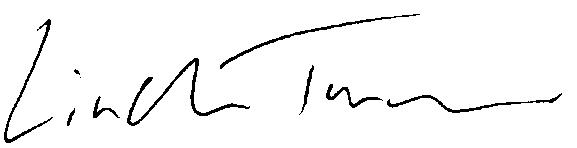
\includegraphics[scale=0.9]{submission/ldt}}\\
% Dr Lincoln Turner

% \vspace{1.5cm}
% \rule{8cm}{1pt}\\
% \raisebox{0.5cm}[0pt][0pt]{
\includegraphics[scale=0.1]{submission/rpa}}\\
% Dr Russell Anderson 

\end{center}

\chapter*{Acknowledgements}

Over the past few years during my PhD, I've been able to learn fascinating things from interesting people, play with fun technological toys, and contribute meaningfully to scientific progress. I could not have done any of this without the support, friendship, and mentorship of many people. The Science Advanced cohort---Rory, Shaun, Lisa, Phil---have been much help getting through everything in my (our, mostly) decade-long visit to Monash. My supervisors---Russ, Lincoln, and Kris---have taught me many things, allowed me freedom to follow my curiosity, and provided endless help on endless matters, including getting this thesis over the finishing line, for which Russ deserves special credit. Thanks also to my sister Rosey for proof-reading on short notice, and to Ana for picking up the slack and tolerating me while I neglected most things that were not thesis.

\cleardoublepage

\newgeometry{left=2.54cm,bottom=1.5in,right=2.54cm,top=1.5in}
\thispagestyle{empty}
\vspace*{\fill}
\begin{center}\emph{To Grandma}
\end{center}
\vspace{\fill}
\restoregeometry

\cleardoublepage

\tableofcontents
% \listoffigures
% \listoftables
\cleardoublepage
\pagenumbering{arabic}


% \section*{Todo list}
% \begin{itemize}
%     \item short caption for all figures for figure list and same for table list.
%     \item Read through looking for using hyphenation in adjectives and not otherwise.
%     \item section -> Section
%     \item acknowledgements
%     \item consistent quote marks -> all to single
%     \item list of abbreviations
%     \item for upright exponential e's
%     \item check for upright imaginary i's
%     \item check for square bracketed todos
%     \item spellcheck whole thing
%     \item confim < 80k words
%     \item put the old what's new bits in the separate chapters
%     \item add to numerics intro mention of the fact that I use these methods in other sections. "review" "Appraisal" "quantitative comparison of benefits" "detailed quantitative appraisal" - most people's numerics sections are sparse - unexamined choice of methods. Defined target audience - new PhD students. Cite Tannor in the intro.  "rapid approach to understanding" for atomic physicists specifically. "Operational"
% Quote numerical recipes on the virtues of simplicity - arm long section of shelf in library got their numerics wrong
%     \item langle rangle fix replace with bras and kets.
%     \item 3D, 2D, \textsc{2d} etc.

% \end{itemize}

% software additions:
% add figures from transfer report and from rottnest talk.
% add experiment script from transfer report - port it to new labscript.
% change titles to be the same as transfer report?

% \chapter{Introduction}\label{chap:introduction}

\lettrine[lines=3]{T}{he subject of study} of this thesis is Bose--Einstein condensation, as well as associated experimental and theoeretical techniques and phenomena in cold atom physics. The following chapters describe my work in a cold atom research group over the past several years, pertaining to apparatus construction, experiment, theory, and software design and development.

Bose--Einstein condensates (\textsc{bec}s) in dilute atomic gases are superfluids that can be created in the lab at extremely low temperatures. This strange state of matter was predicted in 1925 by Bose and Einstein \cite{bose_plancks_1924, einstein_quantentheorie_1925} , first produced experimentally in 1995 \cite{anderson_observation_1995} in a cloud of rubidium atoms, and has since been made out of many other atoms, usually alkali metals \cite{davis_bose-einstein_1995, modugno_bose-einstein_2001, bradley_bose-einstein_1997, weber_bose-einstein_2003}. In a \textsc{bec}, a macroscopic sample of bosonic atoms all occupy the same quantum state, and many of the features of the single particle wavefunctions are exhibited by the cloud as a whole.

[PRACTICAL APPLICATIONS]

Various experimental techniques are used to produce and study Bose--Einstein condensates, many of which exploit of necessitate an understanding of the quantum behaviour of the atomic systems in question. I summarise some of these techniques and the atomic physics principles underlying them in chapter \ref{chap:atomic_physics}.

The fields of Bose--Einstein condensation and cold atoms more generally enjoy a tight coupling between theory and experiment, not least because of the enduring usefulness and accuracy of mean-field theory. In mean-field theory, the quantum matter field operator of the atoms comprising a Bose--Einstein condensate is replaced with its expectation value at each point in space, allowing the entire multi-particle system to be modelled with little more computational complexity than that required to model a single-particle wavefunction.\footnote{mean field theory is accurate in the low-temperature limit, and even then is limited---it is unable for example to correctly model $s$-wave scattering of atoms when two \textsc{bec} wavepackets are collided with each other [CITE], but it is good enough for comparison with a wide range of experiments regardless.} The resulting differential equation---the Gross--Pitaevskii equation---is nonlinear and using it to propagate a condensate wavefunction in time generally requires numerical techniques rather than analytic ones. My favourite numerical methods for doing so (which apply more generally to numerically evolving quantum systems of all kinds) are described in chapter \ref{chap:numerics}. In chapter \ref{chap:numerics} I also develop a variation on fourth-order Runge--Kutta integration which improves on one of its deficiencies for simulating quantum systems. I also present arguments that a fairly sophisticated method of discretising partial differential equations---the finite element discrete variable representation---may offer less computational efficiency that simpler methods for computing solutions of comparable accuracy to the Gross--Pitaevskii and Schr\"odinger wave equations.

As an experimental field, \textsc{bec} research involves the construction of apparatuses capable of implementing the techniques described in chapter \ref{chap:atomic_physics} in order to produce, control, and measure \textsc{bec}s. Chapter \ref{chap:experiment} describes some of the process of constructing such an apparatus, which involves a vacuum system, magnetic coils and optical systems. I present an optical layout for producing magneto-optically trapped $^{87}$Rb atoms (a step on the way to condensation) that I designed and assembled as an exchange student in the group of József Fortágh at the University of T\"ubingen's Physikalisches Institut.

Production, control, and measurement of cold atom systems require more than the necessary optics and magnetic sources to be installed---they must be controllable in a time-accurate way in order to execute the necessary cooling processes, manipulate the system as desired, and observe the results. Production of a condensate takes on the order of tens of seconds, requiring precisely timed pulses of laser light at specific frequencies, sweeps of magnetic field strengths, and frequency sweeps of radio and microwave radiation. This cannot all be done by human experimenters alone, and so requires computer automation of some kind. In chapter \ref{chap:software} I reproduce our publication on a suite of software programs, the \emph{labscript suite}. This software leverages modern software development techniques such as object orientation, abstraction and isolation as well as older principles---such as aspects of the Unix philosophy---to produce a powerful, maintainable, extensible system for designing, running and analysing shot-based experiments on commodity hardware.

[CH6 summary particle velocity]

[CH7 summary wave mixing]

[CH8 summary hidden variables]



TODO:
\begin{itemize}
\item Modify intro to fit ultimate fate of project
\item Move Turbulence discussion to section on vortex tracking
\item summarise forthcoming chapters, specifically pointing out which sections are new results and which are not, and which results are numerics/theory and which are experiment
\item Ensure historical overview does not intrude on theory behind techniques, they should be in the atomic physics section.
\item discuss how BECs are quantum but light is modelled classicaly - Monte Carlo wavefunction methods
\item But MOTS have classical positions.
\item Talk about semiclassical models and allude to my improvement on them with hidden wariables.
\item Discuss how rich the field currently is with applications to precision measurement, quantum information and quantum simulation. Advances are being made in theory, experiment and numerics, in particular with new technology and techniques allowing the latter two to become much more powerful than in the past.
\end{itemize}

As superfluids, \bec s have zero viscosity and as such can support persistent flows. In classical fluid dynamics the absence of viscosity means that a fluid cannot support vorticity,\footnote{This is because the motion of vorticity is described by a diffusion equation---with viscosity as the diffusion constant. When the diffusion constant is zero, there is no way for vorticity to enter the fluid from a boundary in the first place!} and must be irrotational. However, fluid circulation can still occur around points of zero fluid density, known as vortices. In \bec s this circulation is also quantised, in units of $h/m$.

These quantised vortices are topological defects---the phase of the macroscopic wavefunction winds by a multiple of $2\pi$ around them, and is undefined at the center of the vortex core itself.  Quantised vortices were observed in superfluid helium\footnote{In which 10\% or so of the atoms undergo Bose--Einstein condensation.} in the early 1960s \cite{vinen_detection_1961}, and in \bec\ in a dilute atomic gas in 1999 \cite{matthews_vortices_1999}. The formation, dynamics and decay of these vortices are believed to be important for the study of superfluid turbulence \cite{barenghi_quantized_2001}.

This project aims to experimentally realise an imaging method for the real time tracking of quantum vortices in a turbulent $^{41}$K condensate. This will involve ultracold $^{87}$Rb tracer particles which will become bound to vortex lines in the condensate, and which will be imaged repeatedly to track the vortex lines as they move. The imaging of tracer particles to track vortex motion has already proved successful in superfluid helium \cite{bewley_generation_2009, bewley_superfluid_2006, packard_vortex_1982}, and the method of laser cooling and imaging atoms in high resolution with the same laser light has also been successful in cold atom systems \cite{bakr_quantum_2009}. We have tested our method \textit{in-silico} \cite{billington_particle_2010} and from this, expect it to work under a number of assumptions.

\begin{figure}
\begin{center}
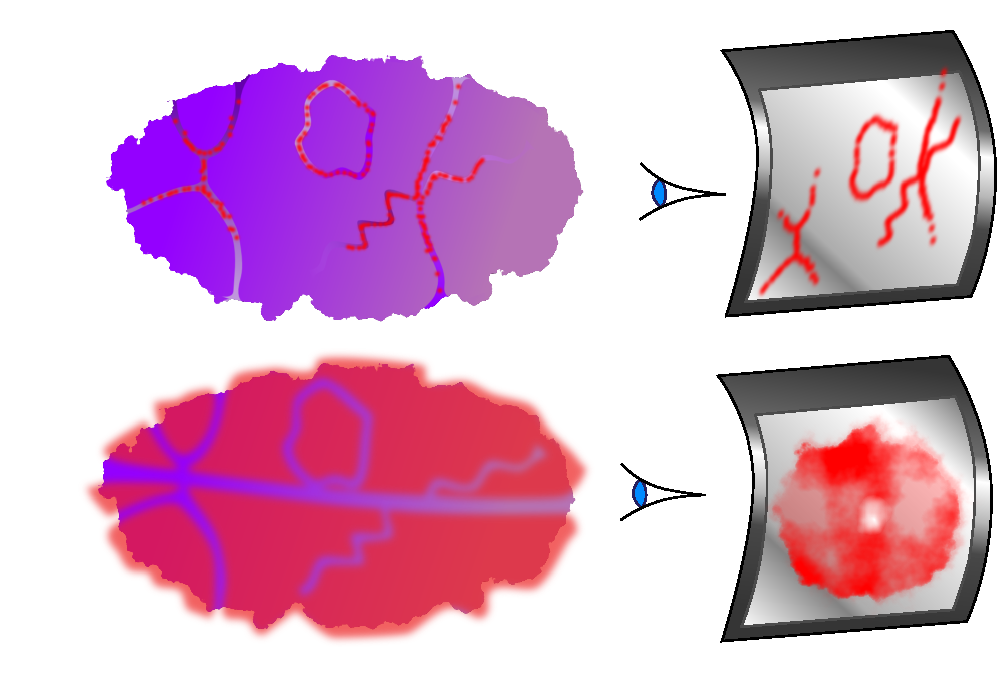
\includegraphics[width=0.6\textwidth]{figures/unsorted/side-on.pdf}
\caption{\label{fig:side-on}Fluorescence imaging of the condensate itself (bottom) makes it difficult to resolve vortices unless they are viewed end-on. The vortex cores are usually smaller than the imaging light's wavelength, and are thus also difficult to resolve unless the cloud is allowed to expand. Imaging tracer particles instead resolves both these problems.}
\end{center}
\end{figure}

If successful, this method will overcome several existing difficulties that other imaging methods face. Since vortices have previously been imaged by resonant absorption imaging of the condensate itself, they are usually viewed with the vortex line perpendicular to the image plane. If not viewed end on, the rest of the cloud obscures the low density of atoms due to the core. One solution to this problem is to slice the condensate into layers, and image them separately \cite{anderson_watching_2001}.

Our method should be able to image vortex lines side-on without destroying the condensate, since the atoms being imaged reside in the vortex core itself rather than the bulk of the condensate. This should make it possible to image the time evolution of Kelvin waves \cite{bretin_quadrupole_2003}, vortex reconnections \cite{leadbeater_sound_2001}, and vortex rings \cite{anderson_watching_2001}.

This \emph{in-situ} imaging of vortex dynamics will allow more types of vortex motion to be imaged. Dynamics of \bec s are usually imaged with a shot-by-shot method, in which repeated experiments with identical initial conditions are imaged destructively after being allowed to evolve for different amounts of time. Whilst this works for many types of dynamics, it fails for experiments that are more sensitive to initial conditions and noise (quantum or otherwise), such as turbulent flow. This includes phenomena which cannot be created reliably in the same initial state, even though the evolution thereafter would be consistent from one experimental run to the next. One such phenomenon is the spontaneous generation of vortices after evaporative cooling \cite{weiler_spontaneous_2008}.

\emph{In-situ} imaging of vortex motion has been achieved previously \cite{freilich_real-time_2010}, by ejecting a fraction of the atoms from the condensate periodically and imaging them. This process is limited by depletion of the condensate, and was also used only to image vortices end-on. The fraction of the condensate being imaged was also allowed to freely expand before being imaged, since vortex cores are otherwise unable to be resolved by the wavelength of light used. Our method requires neither free expansion or depletion of the condensate.

\subsection{Motivation: Turbulence}

It is commonly said that turbulence is one of the greatest unsolved problems of classical physics. But in what sense is it an unsolved problem? Its not a problem at all if your aim is reductionism---the Navier--Stokes equation perfectly describes the evolution of a Newtonian fluid within its domain of validity, and the process of deriving it from the underlying motion of classical particles is completely understood. It's turtles all the way down \cite[p 1]{hawking_brief_1988}; what more could we ask for?

The best comparison to make at this point, I think, is to the field of thermodynamics, for precisely the same statement can be made about the energy content and exchange between systems of particles. Thermodynamics has revealed that despite the chaotic motion of individual particles in an ensemble, definite statements can still be made about the behaviour of the system as a whole, \emph{without having to consider the dynamics of the constituent components in detail}.

This is the kind of solution people have in mind when they speak of `solving' the problem of turbulence. Laws describing the average properties of a fluid without reference to its precise flow field would not simply be interesting as describing turbulence as an emergent phenomenon, but would aid practical computations immensely, which are presently quite difficult. The flow of a turbulent fluid contains detail on such a  wide range of length scales that any finite-element analysis of a system such as say, an aeroplane wing, requires a very high resolution in order to be accurate. Following an estimate of computing power required to simulate a turbulent system down to its smallest length scales, Stanley Corrsin quipped \cite{corrsin_turbulent_1961}:
\begin{quote}
The foregoing estimate  is enough to suggest the use of analog instead of digital  computation; in particular, how about an analog consisting of a tank of water?
\end{quote}

But are we asking for too much? Perhaps the statistical properties of a turbulent fluid fundamentally cannot be decoupled from the finer details. If so, then it is wishful thinking to hope that we might do so.

However there is reason to believe that this is not the case. There are several tantalising results that hint at universal properties that all turbulent flows share, and there is the simple empirical observation that the average flow of turbulent fluids at large scales is reproducible from one experimental run to the next \cite[pp 13, 86]{davidson_turbulence:_2004}.

One of these universal results is Kolmogorov's theory of the statistics of small eddies \cite{kolmogorov_local_1941, spalding_kolmogorovs_1991}. Another is the fact that the rate of energy dissipation via the action of viscosity at small scales \emph{is independent of the viscosity itself} \cite[p 77]{davidson_turbulence:_2004}.

Then there is the Richardson energy cascade \cite{richardson_weather_2007}, in which energy is continually transferred from larger scales to smaller scales. With dissipation at the smallest scales and addition at larger scales, this allows for the existence of `steady state' turbulence.

So far I haven't mentioned superfluids at all, though a superfluid is what this project is studying. There are several interesting aspects of superfluid turbulence that differ from classical turbulence. The most obvious is the absence of viscosity;  another major difference is the quantisation of vortex lines. On scales much larger than the vortex spacing, superfluid turbulence is expected to closely resemble classical turbulence\footnote{At large scales in classical fluids, velocity gradients are small and hence viscosity can be neglected anyway.} \cite{tsubota_energy_2009}. But at smaller scales the energy dissipation mechanism is different, instead involving the production of sound waves via vortex interactions \cite{tsubota_energy_2009, vinen_how_2005}.

In certain 2\textsc{d} geometries, an \emph{inverse cascade} \cite{onsager_statistical_1949, kraichnan_inertial_1967} is predicted to take place in superfluids, whereby energy moves not from large scales to small, but from small to large, clustering quantised vortices of the same circulation direction together. This has not as of yet been observed.

To emphasise the role of vortices in turbulence in general, I will finally give a definition of turbulence, taken from \cite[p 53]{davidson_turbulence:_2004}:
\begin{quote}
Incompressible hydrodynamic turbulence is a spatially complex distribution of vorticity which advects itself in a chaotic manner in accordance with [the vorticity equation\footnote{Which is a transformation of the Navier--Stokes equation for an incompressible fluid into a form in which the vorticity field is center-stage.}]. The vorticity field is random in both space and time, and exhibits a wide and continuous distribution of length and time scales.
\end{quote}

When vorticity exists only in infinitely narrow lines, as it does in superfluid, the vorticity equation mentioned in the above definition reduces to a Biot--Savart type law which can be used to compute the motion of vortices without having to compute the entire flow field.

This is why we are interested in the study of the dynamics of quantised vortices. Unlike in classical fluids, the vortices in superfluids have a definite position and size; there is either a vortex or there is not. This may make it simpler to describe the motion of vortices statistically.

So far experimental studies of superfluid turbulence have mainly been in the context of liquid helium \cite{leggett_superfluidity_1999}; we hope to augment the existing experimental data with that obtained from \bec. The high degree of control afforded over systems of cold atoms allows the superfluid's properties to be tweaked in several ways, creating a larger parameter space in which to study turbulence than that afforded by liquid helium.

\subsection{Experiment control and analysis}

As is typical of an experimental project, much of what goes on day to day is implementation details. It's all very well to say that we want to make a turbulent condensate by pulsing some laser speckle for a few milliseconds, or that we want to ramp down a magnetic field at a certain rate, but how we achieve this in practice? First we have to set up the required equipment---a vacuum system, lasers, optics, magnetic coils, \textsc{rf} antennae. Progress on that front is detailed in section \ref{sec:experimental}.

Once the experiment is set up, we need to be able to control how the system's state changes over time. Components of the system that need to change state during an experiment are typically controlled with analogue and digital electronic signals. Shutters are opened and closed with digital edges; acousto-optical modulators shift the frequency of light passing through them according to a driving \textsc{ac} signal; and magnetic coils create field profiles depending on their current, which in turn depends on the voltage driving their control box. Once we have hardware capable of producing the required digital pulses, voltage ramps, and \textsc{ac} radio frequency signals, running an experiment comes down to programming them and having them execute their programs.

To this end we have created what is essentially a compiler, called \labscript, which takes high level instructions for what the devices should do, and generates the required low-level instructions for all the devices in an experiment, including clocking signals to keep all devices in sync. This is discussed in section \ref{sec:labscript}.

With an experimental run compiled, it needs to be programmed into, and executed on the hardware. This is performed by a program called \blacs, which also provides real-time control of the hardware when not executing pre-compiled experiments.

Experimental runs can take input parameters. For adjusting which values are to be used, and for repeating the same experiment with a range of different parameters, we have a program called \runmanager. \runmanager\ is a graphical front-end for setting these parameters and creating multi-dimensional parameter-space scans.

Two aptly named programs, \lyse\ and \bias, perform analysis of the acquired data as experiments occur. \bias\ interacts with \blacs\ in order to program the camera(s) before a run, and it performs image analysis once the run is complete. \lyse\ is a general purpose analysis system which triggers the execution of user analysis scripts whenever there is new data, computing any results and showing any plots that those scripts contain.

The software components of our control and analysis system are described in more detail in section \ref{sec:software}.


% \setcounter{chapter}{1}
% \chapter{Atomic physics: Experimental techniques and theory}\label{chap:atomic_physics}

\lettrine[lines=3]{B}{ose--Einstein condensates} provide such a tantalising opportunity for studying quantum phenomena not only because of their interesting properties, but also because of the level of control they afford, with parameters able to be tuned and manipulated in order to investigate various regimes. Many of the same techniques which allow experimentalists such control over a \textsc{bec} are also employed in the production of \textsc{bec}.

The main experimental techniques used to create \textsc{bec}s are Doppler cooling, magneto-optical, magnetic, and dipole trapping, polarisation gradient (Sisyphus) cooling, and evaporative cooling. Section~\ref{sec:cooling_and_trapping} is a whirlwind summary of these and a few other experimental techniques. Then in Section~\ref{sec:mean_field_theory}, I'll present some of the theory describing superfluid flow and vortices in \textsc{bec}, which is central to the simulations of vortex tracking presented in Chapter~\ref{chap:velocimetry}. The final section of this chapter, Section~\ref{sec:the_rubidium_D_line}, will construct the detailed theory for describing the internal state of a $^{87}$Rb atom in magnetic and optical fields, considering only the first $L=0$ to $L=1$ excitation is accessible to rubidium's  sole outer-shell electron. The resulting Hamiltonian describes 32 sublevels, and forms the basis of any detailed calculations of laser cooling and trapping.

\section{Cooling, trapping, and manipulating atoms}\label{sec:cooling_and_trapping}

\subsection{Doppler cooling}\label{sec:doppler_cooling}

Doppler cooling, demonstrated in 1978~\cite{wineland_radiation-pressure_1978}, is a consequence of the simple observation that atoms see the wavelength of incident light Doppler shifted depending on their velocity. For example, the electric field of a linearly polarised optical plane wave is
\begin{align}
\vec E \propto \cos(\vec k \cdot \vec r - \omega t),
\end{align}
which for an atom moving with constant velocity $\vec v$ can be written:
\begin{align}
\vec E &\propto \cos(\vec k \cdot \vec v t - \omega t)\\
&= \cos(- \omega_\up{eff} t),
\end{align}
where $\omega_\up{eff} = \omega - \vec k \cdot \vec v$ is the effective angular frequency of the laser as seen by the atom.

This can be used to selectively transfer momentum to only fast-moving atoms, by tuning an incident laser to a slightly lower frequency than that required for a resonant absorption. If six lasers in counter-propagating pairs orthogonal to each other surround a cloud of atoms, an idealised two-level atom theoretically will be cooled close to the \emph{Doppler limit}~\cite[p 58]{metcalf_laser_1999}

\begin{equation}
k_\up{B} T_\up{D} = \frac{\hbar\Gamma}2
\end{equation}

where $\Gamma$ is the line width of the atomic transition. For the effectively two-level cooling transition used for Doppler cooling $^{87}$Rb\footnote{The D$_2$ line, $5\up{S}_{1/2}\rightarrow$ $5\up{P}_{3/2}$, approximately 780 nm.}, this gives $146\,\upmu$K, which is approximately a factor of a thousand too high for Bose-condensation. These atoms are also not trapped.

\subsection{Magneto-optical and magnetic trapping}

Magneto-optical trapping, first demonstrated in 1987~\cite{raab_trapping_1987}, comes from the realisation that a magnetic field can be used to \emph{spatially} vary the detuning from resonance that the atoms in the above-mentioned arrangement of lasers see. This is possible due to the Zeeman effect~\cite{zeeman_influence_1897}, in which the wavelengths of atomic transitions are shifted in a magnetic field.

If a field profile can be found that causes the transition to come closer to resonance as the atoms move away from a central point, then it forms a trap---atoms  that stray too far from the centre will absorb more strongly and be deflected back\footnote{The polarisations of the beams are such that absorption from the inward facing beam occurs, rather than from the one that would accelerate the atom further outward!}.

The field configuration used is an anti-Helmholtz one: two coils opposite each other carrying opposing currents. The resulting magnetic field profile has a zero in the middle and increases in magnitude in all directions.

With the Doppler beams off, this magnetic field still provides a spatially-varying potential, due to the magnetic dipole interaction:

\begin{equation}
V(\vec{r}) = -\vec \mu \cdot \vec B,
\end{equation}
where $\vec\mu$ is the atomic magnetic moment, and $\vec B$ the magnetic field. This only traps some atomic spin states, and has losses due to spin-flips~\cite{brink_majorana_2006} near the field zero.

The optimal magnetic field gradient for forming a magneto-optical trap (\textsc{mot}) is lower than that required to merely hold atoms against gravity, and thus there is little if any magnetic trapping occurring in a \textsc{mot}---the trapping almost entirely results from the position-dependent rate of photon absorption caused by the Zeeman shift due to the magnetic field. To transfer atoms from a \textsc{mot} to a solely magnetic trap, the magnetic field gradient must be increased substantially.

\subsection{Optical dipole trapping}

Optical dipole trapping on the other hand relies on the \emph{dipole force}, in which off-resonant light shifts the energy of the eigenstates of the combined atom-light system, the so called \emph{dressed states}. This energy shift, called the \emph{light shift}, depends on the intensity of the light, and so results in a potential that spatially varies as the intensity of the light. In the limit of large detuning (compared to Rabi frequency), the resulting energy shift for an atom in a ground state (the shift for an excited state is the same but with the opposite sign) is~\cite[p 8]{metcalf_laser_1999}:

\begin{equation}
\Delta E = \frac{\hbar\Omega^2}{4\delta}
\end{equation}

where $\delta$ is the detuning from resonance and the Rabi frequency is
\begin{equation}
\Omega=\frac{E_0}\hbar\matrixel{e}{e\hat{\vec r}}{g},
\end{equation}

where $E_0$ is the amplitude of the light's electric field and  $\matrixel{e}{e\hat{\vec r}}{g}$ is the transition dipole moment between the excited state $\ket{e}$ and ground state $\ket{g}$ of an effectively two-level system. This transition dipole moment can be either for two specific sublevels coupled by a laser, the calculation of which is detailed in Section~\ref{sec:optical_dipole_transitions}, or an overall effective transition dipole moment between two manifolds containing many sublevels, if the detuning much larger compared to the spacing between the sublevels.

With the potential proportional to $E_0^2$, and thus the light's intensity, the force the atom experiences is proportional to the light's intensity gradient. For this reason, the dipole force is also called the \emph{gradient force}. The name \emph{dipole force} comes from the fact that the force can be equivalently understood to arise from the polarisability of atoms in a light field, in which an optically-induced dipole moment gives rise to a force that can be used to trap polarisable materials in optical tweezers~\cite{ashkin_acceleration_1970}.

\subsection{Polarisation gradient cooling}

Polarisation gradient cooling, also called Sisyphus cooling, was proposed in 1989~\cite{dalibard_laser_1989, ungar_optical_1989} to explain experimentally measured cold atom cloud temperatures~\cite{lett_optical_1989} which, at \textsc{nist} in 1988, were found to be well below the expected limit obtainable by the well understood method of Doppler cooling\footnote{As well as to explain other discrepancies between experiments and the theory of Doppler cooling, such as the optimal detuning of light being much greater than predicted.}, one of the few examples of experiments turning out better than expected. A one-dimensional theory has been developed~\cite{dalibard_laser_1989} which has found remarkable agreement with three-dimensional experiments~\cite{salomon_laser_1990}

One common configuration for Sisyphus cooling comprises two counter-propagating laser beams in each spatial dimension, both linearly polarised but with their polarisation angles perpendicular to one another. The optical field resulting from the two beams' superposition has regions of linear polarisation and of both helicities of circular polarisation, and varies between them on a length scale shorter than an optical wavelength.

The effect on multi-level atoms as they move from regions of one circular polarisation to another is that they are pumped alternately from one extreme of their spin-projection state space to the other, alternately climbing and descending potential hills due to the dipole forces from the regions of different polarisations\footnote{If you consider only one polarisation of light, its intensity varies sinusoidally in space, creating a series of potential hills and wells via the dipole force.}. And so, like the Greek legend of Sisyphus\footnote{Polarisation gradient cooling is but one of a family of so called `Sisyphus cooling' methods, all of which involve atoms repeatedly climbing potential hills.}, who was doomed to push a rock uphill for eternity, the atoms are climbing hills repeatedly. Due to the state dependence of the strength of the dipole forces, the atoms climb steeper hills than they descend, and are thus slowed and cooled.

This type of cooling does not work in a magnetic field; the splitting of transition frequencies makes it impossible for an atom to traverse its spin manifold on one laser frequency. For this reason the Sisyphus cooling stage is performed with magnetic fields off, though a sufficiently short period is required such that the atoms can be recaptured when the trapping field is restored.

\subsection{Evaporative cooling}\label{sec:evaporative_cooling}

The final stage of cooling is forced \textsc{rf} evaporative cooling~\cite{hess_evaporative_1986, anderson_observation_1995}, which decreases the temperature of the cloud by systematically removing the hottest atoms. This is performed in a magnetic trap, which as mentioned earlier, only traps certain spin states. Evaporation proceeds by using an \emph{\rf\ knife} to induce spin flips in the atoms. The \textsc{rf} frequency is chosen such that it is only resonant with atoms some distance away from the centre of the trap (via the Zeeman shift). The furthest out atoms are the most energetic, possessing the energy to climb the magnetic potential the furthest. By flipping their spins, these atoms are ejected due to the magnetic field becoming anti-trapping for them.

The cloud is given some time to rethermalise and the knife\footnote{So called because it cuts the tail off the velocity distribution of the atom cloud.} is moved inward where it removes slightly colder atoms. This is repeated until the desired compromise of lower temperature/lower atom number is reached. Usually some method is employed to prevent atoms near the centre of the trap from undergoing spin flips~\cite{brink_majorana_2006} as they move across the field zero. The method used in our lab is to use an optical dipole trap in combination with the magnetic trap~\cite{lin_rapid_2009}, such that the coldest atoms get trapped in the dipole trap which is offset from the magnetic field zero.

\subsection{Feshbach resonances}\label{sec:feshbach}

A Feshbach resonance~\cite{chin_feshbach_2010} is an enhancement of the interparticle interaction strength when a certain magnetic field strength is applied.\footnote{Feshbach resonances can also be induced optically and with \rf\, but magnetic resonances are the most commonly used.} This phenomenon was first studied in the context of ultracold atoms in 1993~\cite{tiesinga_threshold_1993}, experimentally demonstrated in 1998~\cite{inouye_observation_1998}, and is now a staple of cold atom experiments.

\begin{figure}%[htb]
\begin{center}
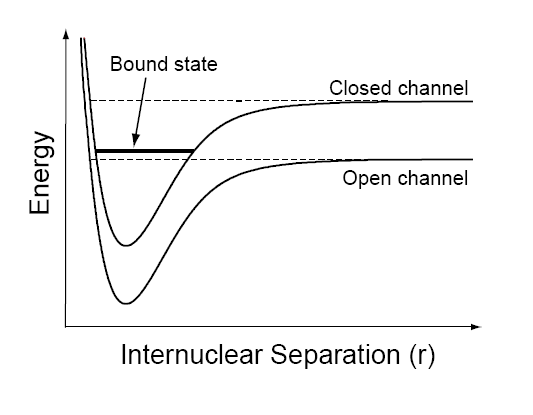
\includegraphics[width=0.5\textwidth]{figures/unsorted/feshbach.png}
\caption{When atoms approach each other with spins aligned, they are in the \emph{open channel}. In this channel they are unbound, but do not have enough energy to be free in the other channel---the \emph{closed channel}. In the close range however, the atoms may have energy corresponding to a bound (molecular) state of the closed channel, a resonance that causes a divergence in the scattering length. The energy difference between the two channels can be tuned with a magnetic field and so these resonances can be induced in a wide range of situations.}\label{fig:feshbach}
\end{center}
\end{figure}

The interparticle interaction mentioned above is
\begin{equation}
g = \frac{2\pi \hbar^2 a}{m_r}
\end{equation}
where $m_r$ is the reduced mass of a pair of the interacting particles, and is dependent on a parameter $a$ called the \emph{s-wave scattering length}, which characterises low energy collisions between atoms. It is sensitive not only to what species of atoms are colliding, but also to their spin states. For each combination of spins, there is a different inter-atomic potential (called a \emph{channel}) which determines the collision dynamics (Figure~\ref{fig:feshbach}).

The resulting scattering length is sensitive to any bound states of this inter-atomic potential which are near the collision energy. If the channels of different spin states are coupled via the hyperfine interaction\footnote{Requiring that the atoms in question have a nuclear magnetic moment.}, then the scattering length is also sensitive to bound states in the channels other than the one the atoms are in when they are far from each other. Due to the Zeeman effect, the energies between the different channels can be shifted with a magnetic field, and so a bound state can be shifted close to the collision energy, which causes the scattering length to diverge.

The end result is that at certain magnetic field strengths we find that atoms are much more strongly attracted to or repelled from each other.

\begin{figure}%[htb]
\begin{center}
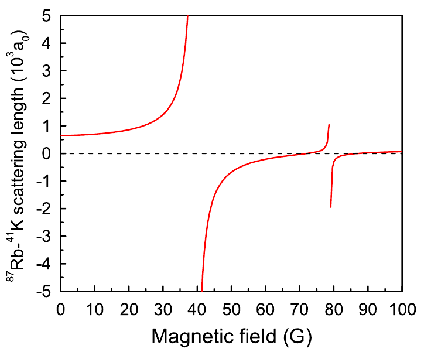
\includegraphics[width=0.5\textwidth]{figures/unsorted/feshKRb.png}
\caption{Predicted interspecies scattering length~\cite{thalhammer_double_2008} as a function of magnetic field strength, for $^{41}$K and $^{87}$Rb both in their lowest energy hyperfine ground state. The $\approx34\unit{G}$ resonance is one of the main reasons for this pair of atoms being used in this project. It has a particularly low field strength and large width compared to most Feshbach resonances. Figure reproduced with permission~\cite{thalhammer_double_2008}, \textcopyright~American Physical Society 2008.}\label{fig:feshKRb}
\end{center}
\end{figure}

A particular Feshbach resonance of interest is shown in~\figref{fig:feshKRb}, and can be used to enhance the interspecies repulsion between $^{87}$Rb and $^{41}$K. The use of this resonance is assumed for the simulations in Chapter~\ref{chap:velocimetry} to trap tracer particles more strongly in vortex cores of a \textsc{bec}.

\section{Mean-field theory: The Gross--Pitaevskii equation and vortices}\label{sec:mean_field_theory}

Bose-condensates are described well by \emph{mean-field} theory, whereby the many-body wavefunction is approximated by a product of identical single-particle wavefunctions. Indeed, that the majority of the atoms are in the same quantum state is one of the defining features of \bec. The effect of interparticle interactions is included as a nonlinear term in the Schr\"odinger equation for the single particle wavefunctions, known as the Gross--Pitaevskii equation:

\begin{align}
\ii\hbar\pdv{t} \Psi(\vec r, t) = \left[-\frac{\hbar^2}{2m}\nabla^2 + V(\vec{\vec r}) + g|\Psi(\vec r, t)|^2\right]\Psi(\vec r, t),
\end{align}
where $g$ characterises the strength of the interparticle interactions\footnote{The nonlinear constant $g$ is usually positive---having the effect of stabilising \bec s by self-repulsion.}, and $\Psi = \sqrt{N}\Psi_\up{single}$ is the single-particle wavefunction scaled by the square root of the number of particles\footnote{Thus giving it the property that $|\Psi|^2$ is the particle density.}.

In the hydrodynamic formulation of quantum mechanics~\cite{madelung_quantentheorie_1927}, the flow velocity of a spatial wavefunction can be defined by considering the probability current to be a product of density and velocity. This allows us to define the superfluid velocity of a \bec\ as
\begin{equation}
\vec v = \frac\hbar m \nabla\phi,
\end{equation}
where $\phi$ is the complex phase of the condensate wavefunction $\Psi$. Integrating this velocity over any closed path $\gamma$ gives us the circulation:
\begin{align}
C &= \frac\hbar m\oint_\gamma\nabla\phi\,ds\\
  &= \frac\hbar m 2\pi n.\qquad n=0,1,2\dots
\end{align}
The fact that the circulation is quantised means that vorticity cannot exist in the condensate except in one-dimensional lines, about which the wavefunction's phase winds by a multiple of $2\pi$. These topological defects are the quantised vortices that are central to the vortex tracking simulations in Chapter~\ref{chap:velocimetry}.

At a vortex core, the atom density of a \bec\ must go to zero. This can be intuitively understood to arise from centrifugal forces, but is also required in order for the wavefunction to be continuous and single-valued across the core. This drop in density in the vicinity of a vortex core is exploited by the method simulated in Chapter~\ref{chap:velocimetry} to trap atoms within the cores.

\section{The $^{87}$Rb $\up{D}$ line}\label{sec:the_rubidium_D_line}

We atomic physicists do our theory work at an intermediate level of abstraction, at which many quantities and systems of interest can be computed and simulated with accurate models using standard quantum mechanics, but with models that are not fully a priori. Instead, the Hamiltonians we feed to the machinery of quantum mechanics encapsulate some of the details we are not interested in or that are too hard to compute, with the link between the underlying layers of reductionism and the higher layer usually provided by experimentally measured values rather than calculations from fundamental physics. In this way we can readily compute results about the atoms we are interested in by treating them as simpler systems than they actually are, with some of the underlying details encapsulated by terms in an effective Hamiltonian for the dynamics that we are interested in.

In this section I will summarise what the $^{87}$Rb $\up{D}$ line looks like from the perspective of a cold atom physicist, building up a Hamiltonian containing all 32 sublevels of the ground and first excited state of $^{87}$Rb including fine structure, hyperfine structure, interaction with a magnetic field, and optical transitions between states. This Hamiltonian is the starting point for any calculations regarding cooling, trapping, and coherent control of $^{87}$Rb, and for other alkali earth metals is much the same.

Many of the details of this section are drawn from references~\cite{steck_rubidium_2015, steck_quantum_2017, metcalf_laser_1999, king_angular_2008, farrell_consistency_1995}, but the reader should be aware that there are considerable conventional and notational differences between different literature sources. What is presented here is summarised and framed in a way that I think is useful to an experimentalist looking to use the theory to make concrete calculations about real systems.

\subsection{Fine structure}\label{sec:fine_structure}

The $^{87}$Rb $\up{D}$ line refers to the first excitation available to the sole outer electron of $^{87}$Rb. Both the ground and excited state of this transition have the same principal quantum number, but different orbital angular momentum quantum numbers. Upon closer inspection, it is not just one transition between a ground state and an excited state---there are two excited states, and the two resulting transitions are called, in order of their transition frequencies, the $\up{D}_1$ and  $\up{D}_2$ lines. Thus the ground and first excited state of $^{87}$Rb are actually a ground state plus two non-degenerate excited states, once we take into account fine structure. The ground state is an $S$ state (electronic orbital angular momentum quantum number $L=0$), called the $S_{1/2}$ state, and the two excited states are $P$ states $(L=1)$, one with the electron spin anti-aligned with its orbital angular momentum (resulting in total angular momentum quantum number $J=1/2$) and one with the electron spin aligned with its orbital angular momentum ($J=3/2$), called the $P_{1/2}$ and $P_{3/2}$ states respectively. In all of these states, $^{87}$Rb's single outer-shell electron occupies an orbital with principle quantum number $n=5$, which for brevity we leave out of the notation. The transition between $S_{1/2}$ and $P_{1/2}$ is called the $\up{D}_1$ line, with experimentally measured (angular) transition frequency $\omega_{\up{D}_1}$, and the transition between $S_{1/2}$ and $P_{3/2}$ is the $\up{D}_2$ line with angular transition frequency $\omega_{\up{D}_2}$. These transition frequencies correspond to optical wavelengths of $\lambda_{\up{D}_1} \approx 795\unit{nm}$ and $\lambda_{\up{D}_2} \approx 780\unit{nm}$\cite{steck_rubidium_2015}.

This fine structure is treated entirely empirically for our purposes, and so our base Hamiltonian for the rubidium $\up{D}$ line, taking into account only fine structure, is simply a statement of the experimentally measured energy differences between the states:

\begin{align}
\hat H_\up{fs} = 
\hbar\omega_{\up{D}_2} \hat1_{P_{3/2}} \oplus
\hbar\omega_{\up{D}_1} \hat1_{P_{1/2}} \oplus
\hat 0_{S_{1/2}},
\end{align}
where $\hat1_{P_{3/2}}$, $\hat1_{P_{1/2}}$, and $\hat 0_{S_{1/2}}$ are identity and zero operators each acting on the subspace of states within the $P_{\frac32}$, $P_{\frac12}$, and $S_{\frac12}$ manifolds respectively, and $\oplus$ is the direct sum.\footnote{Not to be confused with the Kronecker sum, with which it shares notation. The direct sum concatenates matrices as blocks, producing a larger, block-diagonal matrix with dimension equal to the \emph{sum} of the dimensions of the matrices being direct-summed, whereas the Kronecker sum is the regular sum of matrices after each has been multiplied using the Kronecker-product with identity matrices with sizes of the other matrices in the sum, producing matrices with dimension equal to the \emph{product} of those being summed.} The matrix representation $H_\up{fs}$ of $\hat H_\up{fs}$ in the basis in which it is diagonal (which we will call the $\{\ket{L_J}\}$ basis, since $L$ and $J$ are good quantum numbers\footnote{A \emph{good quantum number} is a number that can be used to label (not necessarily uniquely) an energy eigenstate, and on which the energy eigenvalue of that state depends. Saying $J$ and $L$ are good quantum numbers is saying that the eigenstates of the overall Hamiltonian are also eigenstates of $\hat L^2$ and $\hat J^2$, since eigenstates of these two operators can be specified by stating their quantum numbers $L$ and $J$.} for specifying one of the three states, which we write with the spectroscopic notation letter---$S$ or $P$---corresponding to the value of $L$ in place of its numerical value) is
\begin{align}
H_\up{fs}  = 
\left[\begin{matrix}
    \left[\begin{smallmatrix}\ddots &&\\&\hbar\omega_{\up{D}_2}&\\&&\ddots\\\end{smallmatrix} \right]\\
    & \left[\begin{smallmatrix}\ddots &&\\&\hbar\omega_{\up{D}_1}&\\&&\ddots\\\end{smallmatrix} \right]\\
    & &\left[\begin{smallmatrix}\ddots &&\\&0&\\&&\ddots\\\end{smallmatrix} \right]
\end{matrix} \right],
\end{align}
which is a block-diagonal matrix with each block also being a diagonal matrix. We have not yet specified the size of each submatrix---the size of each differs and depends on how many hyperfine and Zeeman sublevels are in that state.

This base Hamiltonian is worth singling out since the energy differences between its three states are orders of magnitude larger than any of the energy differences between hyperfine and Zeeman sublevels within them. When doing any sort of calculations or simulations then, this time-independent Hamiltonian can often be removed from the equations using an interaction picture (see Section~\ref{sec:interaction_picture}), as done in Section~\ref{sec:laser_cooling_simulations} in simulating laser cooling. 

\subsection{Hyperfine structure}\label{sec:hyperfine_structure}

Within each of the $S_{1/2}$, $P_{1/2}$ and $P_{3/2}$ states, the single outer-shell electron's total angular momentum $\hat {\vec J}$ has an interaction with $^{87}$Rb's nuclear angular momentum $\hat{\vec I}$. This results in multiple discrete energy levels depending on the relative orientation of the two separate angular momenta. The interaction Hamiltonian for this hyperfine structure is\footnote{Note that this expression differs from those in the cited references by a factor of $1/\hbar^2$---this is because I define the $\hat{\vec I}$ and $\hat{\vec J}$ angular momentum operators in SI units, rather than in units of $\hbar^2$.}~\cite{steck_rubidium_2015, arimondo_experimental_1977}:
\begin{align}\label{eq:H_hfs}
\hat H_\up{hfs} = \frac{A_\up{hfs}}{\hbar^2} \hat{\vec I} \cdot \hat {\vec J}
+ \frac{B_\up{hfs}}{\hbar^2}\frac
{3(\hat{\vec I}\cdot\hat{\vec J})^2 + \frac32 \hat{\vec I}\cdot\hat{\vec J} - I(I + 1)J(J + 1)}
{2I(2I - 1)J(2J - 1)},
\end{align}
where $J$ is the total angular momentum quantum number of the electron, equal to either $\frac12$ or $\frac32$ depending on which state in the $\up{D}$ line we are considering, $I=\frac32$ is the total angular momentum quantum number of the nucleus, and $A_\up{hfs}$ and $B_\up{hfs}$ are empirically determined coupling constants. Here we see the boundary between the quantities we can calculate with the machinery of quantum mechanics and those that we determine empirically---this expression applies so long as $J$ and $I$ are good quantum numbers,\footnote{$J$ is a good quantum number if the hyperfine splitting is small compared to the spacing between the three states of the $\up{D}$ line, which it is, and $I$ is a good quantum number if the hyperfine splitting is small compared to the energy difference between the ground state and the first \emph{nuclear} excited state, which it most certainly is.} and the two terms are the dipolar and quadrupolar interactions~\cite{arimondo_experimental_1977} between two angular momenta, with the coupling constants determined empirically and encapsulating details that are difficult to compute a priori, such as relativistic effects and the exact shape of the electron orbitals given the presence of inner shell electrons. For the spherically-symmetric $S_{1/2}$ ground state, there is no quadrupolar interaction and so $B_\up{hfs}$ is only non-zero for the two $P$ excited states.\footnote{The quadrupolar term should be explicitly excluded from numerical computations of the hyperfine splitting on the $S_{1/2}$ state, as it contains a division by zero in this case, which may lead to erroneous results even if the term is subsequently multiplied by $B_\up{hfs}=0$.} The values of $A_\up{hfs}$ and $B_\up{hfs}$ for each of the three $L_J$ states of the $\up{D}$ line can be found in~\cite{steck_rubidium_2015}.

For a given state of the $\up{D}$ line, we can construct the matrix representation $\oversetIJ H_\up{hfs}$ of $\hat H_\up{hfs}$ in the $\mathcal{I}\times\mathcal{J}$ basis---which we define as the basis in which both the $z$ vector components $\hat{I}_z$ and $\hat{J}_z$ of $\hat{\vec I}$ and $\hat{\vec J}$ are diagonal---by constructing matrix representations $\oversetIJ{\vec I}$ and $\oversetIJ{\vec J}$ of the operators $\hat{\vec I}$ and $\hat{\vec J}$ in that basis and then applying the expression (\ref{eq:H_hfs}). The overset ${\mathcal{I} \times \mathcal{J}}$ on each of the matrices indicates that the matrix is a representation of its respective operator in the ${\mathcal{I} \times \mathcal{J}}$ basis, so named because its basis vectors can be obtained via a Cartesian product\footnote{The different types of products available for matrices, vectors, operators, spaces, and their sets of basis vectors are rife with subfield-specific conventions and overloaded notation, leading to much ambiguity. Although `Cartesian product' connotes well what I mean here, it is still ambiguous. What I mean is that the ${\mathcal{I} \times \mathcal{J}}$ basis is the set of basis vectors $\{\left.\vec u \otimes \vec v\ \right|\ \vec u \in \mathcal{I}, \vec v\in\mathcal{J}\}$. The notation $\vec u \otimes \vec v$, which is also ambiguous, denotes the Kronecker product of two column vectors, producing a column vector with number of elements equal to the product of the number of elements in each of the two vectors---not the `outer' or `tensor' product, which would produce a matrix.} of the two sets of basis vectors from the $\mathcal{I}$ and $\mathcal{J}$ bases for the two individual nuclear and electronic angular momentum degrees of freedom, in which $\hat{I}_z$ and $\hat{J}_z$ are respectively diagonal.

To construct matrix representations of angular momentum operators in the product space basis ${\mathcal{I} \times \mathcal{J}}$, we first need their matrix representations $\oversetI{\vec I}$ and $\oversetJ{\vec J}$ in the bases of their respective subspaces, which I will write as $\vec I$ and $\vec J$ for brevity. The two operators can then be expanded into the product space by applying a Kronecker product with an appropriate identity matrix to each:
\begin{align}\label{eq:kronecker_identity_I}
\oversetIJ{\vec I}
 &= \vec I \otimes \oversetJ{\mathbb{I}}\\
\label{eq:kronecker_identity_J}
\oversetIJ{\vec J}
&= \oversetI{\mathbb{I}} \otimes \vec J
\end{align}
where $\oversetI{\mathbb{I}}$ is the matrix representation of the identity operator in the $\mathcal{I}$ basis of the nuclear spin degree of freedom, equal to a $(2I+1)\times(2I+1)$ identity matrix, with $\oversetJ{\mathbb{I}}$ defined similarly for the electronic spin degree of freedom.

Each of the two matrices $\vec I$ and $\vec J$ is actually a vector of matrices, one for the angular momentum projection in each of the directions $x$, $y$ and $z$. The procedure for constructing such matrices for arbitrary total angular momentum quantum numbers follows.\footnote{This explicit procedure for constructing the matrix representations of these operators is useful for entering into a programming language to produce programs capable of performing atomic physics calculations for arbitrary total angular momentum quantum number $J$, without having to explicitly enter the angular momentum operators for each value of $J$, which can be tedious and prone to human error.} I will show the procedure for constructing $J_x$, $J_y$ and $J_z$ only for an arbitrary $J$, which is identical to that for computing the vector components of $\vec I$.

For a given total angular momentum quantum number $J$, the vector components of $\vec J$ in the $\mathcal{J}$ basis (the basis in which $J_z$ is diagonal) can be constructed using the raising and lowering operators $\hat J_+$ and $\hat J_-$. Since the action of the raising and lowering operators on an eigenstate of $J_z$ with angular momentum projection quantum number $m_J$ is to produce an adjacent ($m_J \pm 1$) eigenstate multiplied by a constant~\cite[p 192]{sakurai_modern_1994}, this fact can be used to compute the non-zero matrix elements of $\hat J_+$ and $\hat J_-$ in the $\{\ket{m_J}\}$ basis (the basis kets of which we identify with the standard basis vectors\footnote{I will hereafter use the terms `$\mathcal{J}$ basis' and `$\{\ket{m_J}\}$ basis', and similarly for other bases, interchangeably, in the understanding that this identification of standard unit vectors with the basis kets is implied.} for a $2J+1$-dimensional space in order to define the set of concrete basis vectors $\mathcal{J}$):

\begin{align}
\matrixel{m_J + 1}{\hat J_+}{m_J} &= \hbar\sqrt{J(J + 1) - m_J(m_J + 1)}, \qquad -J \leq m_J < J,\\
\matrixel{m_J - 1}{\hat J_-}{m_J} &= \hbar\sqrt{J(J + 1) - m_J(m_J - 1)}, \qquad -J < m_J \leq J,
\end{align}
and therefore compute explicit matrices for $J_+$ and $J_-$ in the $\{\ket{m_J}\}$ basis:\footnote{I'm using the standard convention of ordering the eigenkets $\{\ket{m_J}\}$ in descending order of $m_J$. This is at odds with the computer programming convention of looping over most indices in ascending order, and so care should be taken when constructing these matrices in a computer program.}
\begin{align}
J_+ &=
\left[\begin{smallmatrix}
0 &  \matrixel{J}{\hat J_+}{J - 1} & 0 & \hdots\\
\hdots & 0 & \matrixel{J - 1}{\hat J_+}{J - 2} & 0 & \hdots\\
& & \ddots & \ddots & \ddots\\
 & & \hdots & 0 & \matrixel{ -J + 2}{\hat J_+}{-J + 1} & 0\\
 & & & \hdots & 0 & \matrixel{ -J + 1}{\hat J_+}{-J}\\
 & & & & \hdots & 0\\
\end{smallmatrix} \right],\\
J_- &=
\left[\begin{smallmatrix}
    0 & \hdots \\
    \matrixel{J - 1}{\hat J_-}{J} & 0 & \hdots\\
    0 & \matrixel{J - 2}{\hat J_-}{J - 1} & 0 & \hdots\\
    \hdots & 0 & \matrixel{J - 3}{\hat J_-}{J - 2} & 0 & \hdots\\
    & & \ddots & \ddots & \ddots\\
    & & \hdots & 0 & \matrixel{-J}{\hat J_-}{-J + 1} & 0 \\
\end{smallmatrix} \right],
\end{align}
both of which have non-zero values along only one non-main diagonal adjacent to the main diagonal, and which form a Hermitian conjugate pair (or indeed, a transpose pair, since all elements are real). The matrix representations of $\hat J_x$ and $\hat J_y$ can then be computed by rearranging the defining expressions for $\hat J_+$ and $J_-$;
\begin{align}
\hat J_+ = \hat J_x + \ii \hat J_y,\\
\hat J_- = \hat J_x - \ii \hat J_y,
\end{align}
for $\hat J_x$ and $\hat J_y$, and then applying the result to our matrix representations of $\hat J_+$ and $\hat J_-$ to obtain matrix representations $J_x$ and $J_y$ of $\hat J_x$ and $\hat J_y$ in the $\{\ket{m_J}\}$ basis:
\begin{align}
J_x &= \frac{J_+ + J_-}{2},\\
J_y &= \frac{J_+ - J_-}{2\ii}.
\end{align}
Finally, since $\{\ket{m_J}\}$ is the eigenbasis of $J_z$ with eigenvalues $\{\hbar m_J\}$, the matrix representation of $J_z$ in the $\mathcal{J}$ basis is simply the diagonal matrix of eigenvalues:
\begin{align}
J_z = \left[\begin{smallmatrix}
\hbar J\\
& \hbar (J - 1)\\
& & \ddots\\
& & & \hbar (- J + 1)\\
& & & & -\hbar J\\
\end{smallmatrix} \right].
\end{align} 
We can also construct the matrix representation $J^2$ of the total (squared) angular momentum operator $\hat J^2$ as
\begin{align}
J^2 = J_x^2 + J_y^2 + J_z^2, 
\end{align} 
or equivalently:
\begin{align}
J^2 = J(J+1)\hbar^2 \oversetJ{\mathbb{I}},
\end{align}
since every $m_J$ state is an eigenstate of the $J^2$ operator with eigenvalue $J(J+1)\hbar^2$.

The above prescription can be used to produce matrix representations of angular momentum operators $J_x$, $J_y$, $J_z$ and $J^2$ for any integer or half-integer total angular momentum quantum number $J$. The three components can be considered a vector of matrices, $\vec J$, for the vector angular momentum operator $\hat {\vec J}$. Below is a Python function that computes these matrices as well as the corresponding eigenvectors:

\python{code_listings/angular_momentum_operators.py}

Using the above prescription to construct a matrix representation of the $\hat J$ operator with $J=\frac12$ for the $S_{1/2}$ and $P_{1/2}$ states, or $J=\frac32$ for the $P_{3/2}$ state, and to construct a matrix representation of the $\hat I$ operator with $I=\frac32$, we can explicitly construct a matrix representation of the hyperfine interaction Hamiltonian for any state of the $^{87}$Rb $\up{D}$ line. Remaining is to obtain the matrix representations of the two operators in the $\mathcal{I}\times\mathcal{J}$ product space basis using~\eqref{eq:kronecker_identity_I} and~\eqref{eq:kronecker_identity_J}, and then we can apply~\eqref{eq:H_hfs} to our matrices to obtain the matrix representation $\oversetIJ H_\up{hfs}$ of $\hat H_\up{hfs}$ for a given $J$ corresponding to one of the three states on the $\up{D}$ line:
\begin{align}\label{eq:H_hfs_matrix}
\oversetIJ H_\up{hfs} = \frac{A_\up{hfs}}{\hbar^2}
\oversetIJ{\vec I} \cdot
\oversetIJ{\vec J}
+ \frac{B_\up{hfs}}{\hbar^2}\frac
{3(\oversetIJ{\vec I}\cdot
\oversetIJ{\vec J})^2
+ \frac32 \oversetIJ{\vec I}\cdot
\oversetIJ{\vec J}
 - I(I + 1)J(J + 1)}
{2I(2I - 1)J(2J - 1)},
\end{align}
where the products of vector components within the dot products are computed with ordinary matrix multiplication. Alternatively, one can use the matrices in their individual subspaces rather than their equivalents in the product space, so long as one interprets the dot products as `Kronecker dot products':
\begin{align}\label{eq:H_hfs_matrix_kron}
\oversetIJ H_\up{hfs} = \frac{A_\up{hfs}}{\hbar^2}
\vec I \krondot \vec J
+ \frac{B_\up{hfs}}{\hbar^2}\frac
{3(\vec I \krondot \vec J)^2
+ \frac32 \vec I \krondot \vec J
 - I(I + 1)J(J + 1)}
{2I(2I - 1)J(2J - 1)},
\end{align}
where $\krondot$ is the Kronecker dot product:
\begin{align}
\vec I \krondot \vec J \equiv I_x \otimes J_x + I_y \otimes J_y + I_z \otimes J_z.
\end{align}

In the above way one can construct an explicit matrix representation of $\hat H_\up{hfs}$ in the $\mathcal{I} \times \mathcal{J}$ basis for the hyperfine interaction for a given $L_J$ state of the $\up{D}$ line.

\subsubsection{Column vectors in the $\mathcal{I}\times\mathcal{J}$ basis}

Because the matrix representations $\vec I$ and $\vec J$ of the electron and nuclear angular momentum operators were constructed in the $\{\ket{m_I}\}$ and $\{\ket{m_I}\}$ bases of their respective subspaces, the matrices we have constructed are in the basis $\mathcal{I}\times\mathcal{J}$ with basis vectors:
\begin{align}
\mathcal{I}\times\mathcal{J} = \left\{\left. \ket{m_I\ m_J} \ \right| \ \ket{m_I} \in \{\ket{m_I}\}, \ket{m_J} \in \{\ket{m_J}\}\right\},
\end{align}
where $\ket{m_I\ m_J} = \ket{m_I} \otimes \ket{m_J}$. The vector representation $\vec\psi$ of a state vector $\ket{\psi}$ in this basis is
\begin{align}
\vec \psi = \left[\begin{smallmatrix}
\braket{m_I=I\ m_J=J}{\psi}\\
\braket{m_I=I\ m_J=J-1}{\psi}\\
\vdots\\
\braket{m_I=I\ m_J=-J}{\psi}\\
\braket{m_I=I-1\ m_J=J}{\psi}\\
\braket{m_I=I-1\ m_J=J-1}{\psi}\\
\vdots\\
\vdots\\
\braket{m_I=-I\ m_J=-J}{\psi}\\
\end{smallmatrix}\right].
\end{align}
The hyperfine Hamiltonian is not diagonal in the $\{\ket{m_I\ m_J}\}$ basis. The basis in which it is diagonal---the $\{\ket{F\ m_F}\}$ basis---will be discussed in Section~\ref{sec:the_F_mF_basis}.

\subsection{Zeeman sublevels}\label{sec:zeeman_sublevels}

The states differing only in their $m_F$ quantum numbers---called Zeeman sublevels---are degenerate in energy with respect to the hyperfine Hamiltonian, but an external magnetic field lifts this degeneracy. The Zeeman effect~\cite{zeeman_influence_1897, steck_rubidium_2015} results in an energy shift proportional to the external magnetic field $\vec B$ and to a system's magnetic moment $\vec \mu$:
\begin{align}
V = - \vec\mu\cdot\vec B.
\end{align}
Our atom is a composite particle, made of a nucleus with its own intrinsic magnetic moment, an electron with its own intrinsic magnetic moment as well, and a contribution from the orbital motion of the electron about the nucleus. Each magnetic moment is proportional to the angular momentum of the subsystem in question, with the proportionality constants, called Land\'e g-factors written as dimensionless multiples of $-\mu_B/\hbar$, where $\mu_B$ is the Bohr magneton.\footnote{We are using the sign convention that defines the Land\'e $g$-factor $g_J$ for the electron as positive.} Since $J$ is a good quantum number so long as energy shifts are smaller than the (large) energy spacing between the three $L_J$ states of the $\up{D}$ line, on the level we work we don't consider the electron spin and orbital angular momenta separately, rather we encapsulate them with a single, empirically determined Land\'e g-factor $g_J$~\cite{steck_rubidium_2015} for the magnetic moment of the electron in each of the three $L_J$ states. Similarly we consider the nucleus as a single spin with an experimentally determined $g_I$~\cite{steck_rubidium_2015}, resulting in a Zeeman Hamiltonian:
\begin{align}
\hat H_\up{Z} & = -\hat{\vec \mu} \cdot \vec B\\
&= -\left(\hat{\vec \mu}_I + \hat{\vec \mu}_J\right) \cdot \vec B\\
&=\left(\frac{g_I\mu_B}{\hbar} \hat{\vec I} + \frac{g_J\mu_B}{\hbar} \hat{\vec J}\right) \cdot \vec B.\label{eq:H_Z}
\end{align}
Separate $g_S$ and $g_L$ values are known and can be used in two terms instead of the one containing $\hat{\vec J}$ above if $J$ is not a good quantum number, but in the regime we work that is not usually the case (and if it were, the fine and hyperfine structure Hamiltonians above would also be inadequate since they assume that $J$ is a good quantum number). If $J$ is a good quantum number then it is more accurate to use the above expression with empirically measured $g_J$ values, since they encapsulate QED effects and corrections due to the multi-electron structure of $^{87}$Rb that are not captured by the simple Zeeman Hamiltonian with separate $\hat{\vec S}$ and $\hat{\vec L}$ terms~\cite{steck_rubidium_2015}. 

If the energy shifts from the Zeeman effect are small compared to the hyperfine spitting, then $F$ (the total spin quantum number, defined in the next section) is a good quantum number and a given hyperfine level can be treated as a single magnetic moment subject to the Zeeman Hamiltonian:
\begin{align}
\hat H_\up{Z\,lin} = \frac{g_F\mu_B}{\hbar} \hat{\vec F} \cdot \vec B,
\end{align}
where~\cite{steck_rubidium_2015}
\begin{align}
g_F = g_J\frac{F(F+1) - I(I+1) + J(J+1)}{2F(F+1)}
    + g_I\frac{F(F+1) + I(I+1) - J(J+1)}{2F(F+1)}.
\end{align}
The direction in which each Zeeman sublevel shifts in energy for small magnetic fields is depicted in~\figref{fig:D_line}. Experimentally, Zeeman shifts that depart from this linear regime are not infrequently encountered, and so it is an approximation that cannot always be made.

An explicit matrix representation $\oversetIJ{H}_\up{Z}$ of $\hat H_\up{Z}$ in the $\{\ket{m_I\ m_J}\}$ basis for each of the three $L_J$ states of the $\up{D}$ line can be constructed by applying~\eqref{eq:H_Z} to the matrix representations of $\hat{\vec I}$ and $\hat{\vec J}$ in that basis: 
\begin{align}\label{eq:Zeeman_hamiltonian}
\oversetIJ{H}_\up{Z} &= -\oversetIJ{\vec\mu}\cdot \vec B,
\end{align}
where
\begin{align}\label{eq:magnetic_moment_operator}
\oversetIJ{\vec\mu} &=
-\frac{g_I\mu_B}{\hbar} \oversetIJ{\vec I}
- \frac{g_J\mu_B}{\hbar} \oversetIJ{\vec J}\\
&= -\frac{g_I\mu_B}{\hbar} \vec I \otimes \oversetJ{\mathbb{I}}
- \frac{g_J\mu_B}{\hbar} \oversetI{\mathbb{I}} \otimes \vec J.
\end{align}

\subsection{Putting it all together: the $\{\ket{F\ m_F}\}$ basis}\label{sec:the_F_mF_basis}

So far we have described how to construct a matrix representation of the fine structure Hamiltonian for the three $L_J$ states of the $^{87}$Rb $\up{D}$ line, as well as matrix representations of each state's hyperfine and Zeeman Hamiltonians, these latter two in the same $\{\ket{m_I\ m_J}\}$ basis. In the subspaces of each of the three $L_J$ states then, we can sum together the hyperfine and Zeeman Hamiltonians to form (a matrix representation of) a Hamiltonian that takes interactions into account:
\begin{align}
\oversetIJ H_{P_{3/2}} &=
  \oversetIJ H_{\up{hfs}\,P_{3/2}} + \oversetIJ H_{\up{Z}\,P_{3/2}},\\
\oversetIJ H_{P_{1/2}} &=
  \oversetIJ H_{\up{hfs}\,P_{1/2}} + \oversetIJ H_{\up{Z}\,P_{1/2}},\\
\oversetIJ H_{S_{1/2}} &=
  \oversetIJ H_{\up{hfs}\,S_{1/2}} + \oversetIJ H_{\up{Z}\,S_{1/2}},
\end{align}
where the subscripts $P_{3/2}$, $P_{1/2}$, and $S_{1/2}$ on the terms on the right hand side indicate that the expressions for the matrix elements of the hyperfine and Zeeman Hamiltonians are to be evaluated using the specific values of $J$, $A_\up{hfs}$, $B_\up{hfs}$, and $g_J$ relevant to that state. The total Hamiltonian for the $\up{D}$ line including fine structure, hyperfine structure and the Zeeman interaction is then
\begin{align}
\hat H &= \hat H_\up{fs} +
    \left(\hat H_{P_{3/2}} \oplus \hat H_{P_{1/2}} \oplus \hat H_{S_{1/2}} \right)\\
\Rightarrow \hat H &= 
\left(\hbar\omega_{D_2}\hat 1_{P_{3/2}} + \hat H_{P_{3/2}}\right) \oplus
\left(\hbar\omega_{D_1}\hat 1_{P_{1/2}} + \hat H_{P_{1/2}}\right) \oplus \hat H_{S_{1/2}},
\end{align}
the matrix representation of which in the $\{\ket{L\ J\ m_I\ m_J}\}$ basis is the block diagonal matrix
\begin{align}
\oversetIJ H_{\up{D}\,^{87}\up{Rb}}  = 
\left[\begin{matrix}
    \left[\begin{smallmatrix}
        \hbar\omega_{\up{D}_2} + \oversetIJ  H_{P_{3/2}}\\
    \end{smallmatrix} \right]\\
    & \left[\begin{smallmatrix}
        \hbar\omega_{\up{D}_1} + \oversetIJ  H_{P_{1/2}}\\
      \end{smallmatrix} \right]\\
    & &\left[\begin{smallmatrix}
        \oversetIJ  H_{S_{1/2}}\\
        \end{smallmatrix} \right]\\
\end{matrix} \right],
\end{align}
where addition of scalars with matrices implies the addition of a scalar multiple of the appropriately sized identity matrix.

While $\oversetIJ H_{\up{D}\,^{87}\up{Rb}}$ is a block diagonal matrix, each of the three submatrices is not diagonal, since $m_I$ and $m_J$ are not good quantum numbers for the hyperfine interaction (though they are good quantum numbers for the Zeeman interaction and hence $\oversetIJ  H_{\up{D}\,^{87}\up{Rb}}$ becomes approximately diagonal at high magnetic field). Once one has constructed $\oversetIJ  H_{\up{D}\,^{87}\up{Rb}}$ or its submatrices, there are two other bases one might consider transforming the submatrices into depending on the circumstances. One is the $\Sigma\mathcal{F} = \{\ket{F\ m_F}\}$ basis\footnote{The name $\Sigma\mathcal{F}$ refers to the fact that this is the basis that lends itself to the interpretation of the total space being the direct sum of subspaces, each of which has a well defined $F$ quantum number. So if $\mathcal{I}\times\mathcal{J}$ is a basis for a product space with $(2I+1)\times(2J+1)$ dimensions, then $\Sigma \mathcal{F}$ is a basis for a \emph{sum space} with $\sum_i (2F_i + 1)$ dimensions, where $F_i$ ranges from $\abs{I-J}$ to $I+J$ in integer steps. The product and sum bases have the same dimensionality and span the same space, so the difference is only in the identification and composition of their component subspaces.}, in which the matrix representation of the hyperfine interaction is diagonal. The matrix representation of the Zeeman Hamiltonian is also approximately diagonal in the $\{\ket{F\ m_F}\}$ basis, so long as one is in the linear Zeeman regime. Furthermore, the transition dipole moments for optical transitions are most easily calculated in the $\{\ket{L_J\ F\ m_F}\}$ basis, as we'll see in the next subsection. For these reasons the $\{\ket{F\ m_F}\}$ basis is the most commonly used and referred to.

The $\{\ket{F\ m_F}\}$ basis is defined as the simultaneous eigenbasis of the $\hat F^2$ and $\hat F_z$ operators, which are the total (squared) and $z$ component of the total angular momentum operator $\hat{\vec{F}} = \hat{\vec{I}} + \hat{\vec{J}}$, the matrix forms $F^2$ and $F_z$ of which in the $\ket{m_I\ m_J}$ basis can be constructed from the matrix forms of the individual angular momentum operators:
\begin{align}
\oversetIJ{\vec F} &= \oversetIJ{\vec I} + \oversetIJ{\vec J}\nonumber\\
& = \vec I \otimes \oversetJ{\mathbb{I}} + \oversetI{\mathbb{I}} \otimes \vec J;\\
\oversetIJ{F_z} &= \oversetIJ {I_z} + \oversetIJ {J_z}\nonumber\\
& = I_z \otimes \oversetJ{\mathbb{I}} + \oversetI{\mathbb{I}} \otimes J_z;\\
\oversetIJ {F^2} &= \oversetIJ{\vec F}\cdot\oversetIJ{\vec F}.
\end{align}
The $\{\ket{F m_F}\}$ basis allows the eigenstates of the hyperfine interaction to be labelled with $F$ and $m_F$ quantum numbers. For a state of the $^{87}$Rb $\up{D}$ line with electron total angular momentum quantum number $J$, there are $1+J+I - \abs{(I - J)}$ hyperfine levels, with $F$ quantum numbers running from $\abs{I - J}$ to $I + J$. Within each hyperfine level there are $2F + 1$ degenerate states with different $m_F$ quantum numbers ranging from $-F$ to $F$. This results in a total of 32 possible states for the rubidium $\up{D}$ line, a schematic of which is shown in~\figref{fig:D_line}.

\begin{figure}%[htb]
\begin{center}
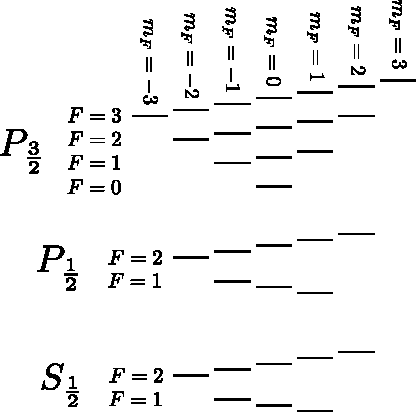
\includegraphics[width=0.5\textwidth]{figures/atomic_physics/D_line.pdf}
\caption{The 32 states of the $^{87}$Rb $\up{D}$ line, ordered vertically by energy (not to scale) in a small magnetic field. At zero magnetic field, Zeeman sublevels sharing a common $F$ quantum number and within the same hyperfine level are degenerate. At small magnetic fields this degeneracy is lifted, with state energies shifting in the directions depicted. However, $F$ is no longer a good quantum number at non-zero magnetic field, as most of the non-degenerate sublevels are actually equal to linear combinations of two states of different $F$ quantum numbers. Nevertheless at low magnetic fields the states are labelled using $F$ anyway, since one $F$ state dominates the linear combination, and at higher magnetic fields the states are labelled using an index $\alpha$, equal to the value of $F$ of the state that would dominate the superposition if the field were smoothly reduced to zero. $m_F$ remains a good quantum number at non-zero magnetic field however, and so at all fields a state can be specified by the numbers $L$, $J$, $\alpha$ (equal to $F$ at small field) and $m_F$.} \label{fig:D_line}
\end{center}
\end{figure}

To transform each submatrix between the $\{\ket{m_I\ m_J}\}$ and $\{\ket{F\ m_F}\}$ bases, we use a unitary matrix whose elements are Clebsch--Gordan coefficients, each defined as the inner product of a $\ket{F\ m_F}$ state with a $\ket{m_I\ m_J}$ state (written in full as $\ket{I\ m_I\ J\ m_J}$), and calculable as~\cite{steck_rubidium_2015}
\begin{align}\label{eq:ClebschGordanCoeffs}
\braket{I\ m_I\ J\ m_J}{F\ m_F} &=
(-1)^{I - J + m_F}\sqrt{2F + 1}
\left(\begin{matrix}
I & J & F\\
m_I & m_J & -m_F\\
\end{matrix}\right)
\end{align}
where the object in parentheses is a Wigner $3$-j symbol. The Clebsch--Gordan coefficients are real: $\braket{F\ m_F}{I\ m_I\ J\ m_J} = \braket{I\ m_I\ J\ m_J}{F\ m_F}$, and are zero unless $m_I + m_J = m_F$.
Given that the possible range of the $F$ quantum number is from $\abs{I - J}$ to $I + J$, and the possible range of $m_F$ quantum numbers is from $-F$ to $F$ for each $F$ (both in integer steps), an explicit construction of the unitary matrix $U_\up{CG}$ of Clebsch--Gordan coefficients, in the convention where the column vectors in the $\{\ket{F\ m_F}\}$ basis have $F$ running from its highest value to lowest from top to bottom, and $m_F$ also running from highest to lowest within each value of $F$, (omitting $I$ and $J$ for brevity) is
\begin{align}
U_\up{CG} = \left[\begin{smallmatrix}
\braket{m_I=I\ m_J=J}{F=I+J\ mF=F} & \hdots &
\braket{m_I=I\ m_J=J}{F=I+J\ m_F=-F} & \hdots &\hdots &
\braket{m_I=I\ m_J=J}{F=\abs{I - J}\ m_F=-F}\\
\vdots\\
\braket{m_I=-I\ m_J=J}{F=I+J\ mF=F} & & \ddots & & & \vdots\\
\vdots\\
\vdots\\
\braket{m_I=-I\ m_J=-J}{F=I+J\ mF=F} & & \hdots & & &
\braket{m_I=-I\ m_J=-J}{F=\abs{I - J}\ m_F=-F}\\
\end{smallmatrix}\right].
\end{align}
This the matrix that takes vectors from the $\{\ket{F\ m_F}\}$ basis to the $\{\ket{m_I\ m_J}\}$ basis, so its Hermitian conjugate $U^\dagger_\up{CG}$ is needed for the inverse transformation (which is equal to the transpose since the matrix elements are real). Within the convention we're using to order the matrix elements, the vector representation $\vec\psi$ of a state vector $\ket{\psi}$ in the $\{\ket{F\ m_F}\}$ basis of one of the $L_J$ states is
\begin{align}
\vec \psi = \left[\begin{smallmatrix}
\braket{F=I+J\ m_F=F}{\psi}\\
\braket{F=I+J\ m_F=F-1}{\psi}\\
\vdots\\
\braket{F=I+J\ m_F=-F}{\psi}\\
\braket{F=I+J-1\ m_F=F}{\psi}\\
\braket{F=I+J-1\ m_F=F-1}{\psi}\\
\vdots\\
\vdots\\
\braket{m_F=\abs{I-J}\ m_F=-F}{\psi}\\
\end{smallmatrix}\right].
\end{align}

Each submatrix of the total Hamiltonian for the $\up{D}$ line can be transformed into its $\{\ket{F\ m_F}\}$ basis by using a unitary matrix of Clebsch--Gordan coefficients with the appropriate value of $J$, yielding a total Hamiltonian for the $^{87}$Rb $\up{D}$ line in the $\{\ket{L_J\ F\ m_F}\}$ basis:
\begin{align}
\oversetF{H}_{\up{D}\,^{87}\up{Rb}}
&= \left[\begin{matrix}
    \left[\begin{smallmatrix}
        \hbar\omega_{\up{D}_2}+U^\dagger_{\up{CG}\,3/2}
        \oversetIJ H_{P_{3/2}}U_{\up{CG}\,3/2}\\
        \end{smallmatrix} \right]\\
    & \left[\begin{smallmatrix}
        \hbar\omega_{\up{D}_1}+U^\dagger_{\up{CG}\,1/2}
        \oversetIJ H_{P_{1/2}}U_{\up{CG}\,1/2}\\
      \end{smallmatrix} \right]\\
    & &\left[\begin{smallmatrix}
        U^\dagger_{\up{CG}\,1/2} 
        \oversetIJ H_{S_{1/2}} U_{\up{CG}\,1/2}\\
    \end{smallmatrix} \right]\\
\end{matrix} \right]\\
&= \left[\begin{matrix}
    \left[\begin{smallmatrix}
        \hbar\omega_{\up{D}_2} +
        \oversetF H_{P_{3/2}}\\
        \end{smallmatrix} \right]\\
    & \left[\begin{smallmatrix}
        \hbar\omega_{\up{D}_1} +
        \oversetF H_{P_{1/2}}\\
      \end{smallmatrix} \right]\\
    & &\left[\begin{smallmatrix}
        \oversetF H_{S_{1/2}}\\
    \end{smallmatrix} \right]\\
\end{matrix} \right]
\end{align}
where the additional subscripts on the unitary matrices indicates the value of $J$ used in its construction. Armed with the $\{\ket{F, m_F}\}$ basis, we have little remaining reason to use the $\{\ket{m_I\ m_J}\}$ basis any more.

Here is a recap of what we have taken into account with our model of the Rubidium $\up{D}$ line:
\begin{itemize}
    \item Orbital angular momentum: the two lowest quantum numbers $L=0$ and $L=1$ of the electron's orbital angular momentum: this yields the $S$ ground state and $P$ excited state.
    \item Fine structure: the two possible orientations of the electron's spin with respect to its orbital angular momentum. This splits the $P$ excited state into two states, $P_{1/2}$ and $P_{3/2}$, and leaves the $S$ ground state as the single state $S_{1/2}$. The energies of these three states are determined entirely empirically---without any modelling of the fine structure.
    \item Hyperfine structure: The possible orientations of the electron's total angular momentum with respect to the nuclear angular momentum. This splits each state so far into $1+J+I - \abs{(I - J)}$ hyperfine states. The hyperfine interaction is treated semi-empirically, using an analytic form of the hyperfine interaction but with empirically determined coupling constants within each of the three $L_J$ states of the $\up{D}$ line. 
    \item Zeeman effect: the possible orientation of the angular momenta $\hat{\vec I}$ and $\hat{\vec J}$---or at low field their sum $\hat{\vec F}$---onto an external magnetic field. The Zeeman Hamiltonian is modelled analytically, but with empirically determined Land\'e $g$ factors for each of the three $L_J$ states of the $\up{D}$ line. 
\end{itemize}

The above considerations allow us to construct a Hamiltonian, as a concrete matrix representation, for all 32 possible states of the rubidium $\up{D}$ line in a fixed magnetic field, in a basis in which it is diagonal for the case of zero magnetic field. In a non-zero magnetic field, one can analytically diagonalise the $S_{1/2}$ and $P_{1/2}$blocks of this matrix using the Breit--Rabi formula
\citeleft\citen{steck_quantum_2017}, p.~347;~\citen{breit_measurement_1931}\citeright, but analytic treatment of the $P_{3/2}$ block is considerably more involved and it is generally diagonalised numerically. At non-zero magnetic field, $F$ ceases to be a good quantum number, but states are nonetheless labelled using a variable $\alpha$, defined as the value of $F$ a state \emph{would} have if the magnetic field were reduced to zero. $m_F$ remains a good quantum number however, and thus at non-zero magnetic field the $\{\ket{\alpha\ m_F}\}$ basis, is the one in which the Hamiltonian is diagonal, with the transformation between it and the $\{\ket{F\ m_F}\}$ basis requiring numerical diagonalisation.

If the magnetic field is static, then this Hamiltonian $\hat{H}_{\up{D}\,^{87}\up{Rb}}$ is a time-independent Hamiltonian, to which additional time-dependent Hamiltonians can be added to take into account optical or $\textsc{rf}$ transitions, detailed below. In a dynamic magnetic field, only $\hat H_\up{hfs}$ is time-independent, in which case the Zeeman Hamiltonian will also be part of the time-dependent part of the Hamiltonian. This has implications for the use of an interaction picture (described in Section~\ref{sec:interaction_picture}), in which the time-independent part of a Hamiltonian can be analytically removed from the equations of motion, which can make further computations more tractable both analytically and numerically.

\subsection{Optical dipole transitions}\label{sec:optical_dipole_transitions}

Optical transitions due to laser fields appear as off-diagonal matrix elements in the $\{\ket{F\ m_F}\}$ basis\footnote{The matrix elements can be obtained in the $\{\ket{\alpha\ m_F}\}$ basis at non-zero magnetic field via the numerically computed transformation mentioned in the previous subsection.}. A given laser of a certain polarisation may give rise to non-zero transition matrix elements between several different pairs of states, depending on selection rules.

The potential the outer electron of rubidium is subject to in a classical electric field is the electric dipole potential~\cite{metcalf_laser_1999, steck_quantum_2017}:
\begin{align}
\hat H_\up{d} = -\hat{\vec d}\cdot\vec E,
\end{align}
where $\vec E$ is the classical electric field and $\hat{\vec d}$ is the electric dipole operator:
\begin{align}
\hat{\vec d} = -e\vec{\hat r},
\end{align}
which gives the electric dipole of the atom in terms of the electron's charge $-e$ and its position operator (with respect to the nucleus) $\hat{\vec r}$. A single matrix element of $\hat H_\up{d}$ for coupling an initial state $\ket{L_J\ F\ m_F}$ to a final state $\ket{L^\prime_{J^\prime}\ F^\prime\ m_F^\prime}$ is therefore:
\begin{align}\label{eq:electric_dipole_potential}
\matrixel{L^\prime_{J^\prime}\ F^\prime\ m_F^\prime}{\hat H_\up{d}}{L_J\ F\ m_F} = 
\matrixel{L^\prime_{J^\prime}\ F^\prime\ m_F^\prime}{e\vec{\hat r}\cdot\vec E}{L_J\ F\ m_F},
\end{align}
which we will abbreviate as
\begin{align}
\matrixel{n^\prime}{\hat H_\up{d}}{n} = 
\matrixel{n^\prime}{e\vec{\hat r}\cdot\vec E}{n},
\end{align}
writing the initial state $\ket{L_J\ F\ m_F}=\ket{n}$ and final state $\ket{L^\prime_{J^\prime}\ F^\prime\ m_F^\prime}=\ket{n^\prime}$, encapsulating the set of quantum numbers as a single index\footnote{The choice of the symbol $n$ is unrelated to the principal quantum number, which does not vary between the states of the $\up{D}$ line.} for the state.

\subsubsection{Plane waves}

The electric field of a plane wave of amplitude $E_0$, polarisation unit vector $\hat{\vec\varepsilon}$ and angular frequency $\omega$ can be written:
\begin{align}\label{eq:complex_plane_wave}
\vec E(\vec r, t) = \frac{E_0}2
\left(\hat{\vec\varepsilon} \ee^{\ii(\vec k \cdot \vec r - \omega t)}
+ \hat{\vec\varepsilon}^* \ee^{-\ii(\vec k \cdot \vec r - \omega t)} \right),
\end{align}
where $^*$ is complex conjugation, which in the case of a real valued polarisation unit vector $\hat{\vec\varepsilon}$ does nothing, making the above equal to a cosine wave $E_0\hat{\vec\varepsilon}\cos(\vec k \cdot \vec r - \omega t)$ as expected for a linearly polarised plane wave. However,~\eqref{eq:complex_plane_wave} also allows for arbitrary circular or elliptical polarisation, if $\hat{\vec\varepsilon}$ is allowed to have complex components. This comes with the caveat, however, that the amplitude $E_0$ is a misnomer in these cases and no longer corresponds to any actual amplitude. For example, a circularly polarised plane wave propagating in the $z$ direction constructed using complex polarisation vector $\hat{\vec\varepsilon}=\mp(\hat{\vec{x}} \pm i \hat{\vec y})/\sqrt{2}$) and `amplitude' $E_0$ actually has an electric field vector with constant magnitude $E_0/\sqrt{2}$. The `amplitude' $E_0$ in~\eqref{eq:complex_plane_wave} is actually equal to $\sqrt{2}E_\up{rms}$ and thus only equal to the peak electric field strength in the case of linear polarisation. Using the intensity of the beam\footnote{Not to be confused with the nuclear spin $I$, distinguishable by context.} $I=\varepsilon_0 c E_\up{rms}^2$ instead, which is less ambiguous and more relatable to experimentalists~\cite{king_angular_2008}, resolves this potential confusion:\footnote{One possible confusion of many given the diverse notational and conventional differences throughout the literature.}
\begin{align}\label{eq:complex_plane_wave_intensity}
\vec E(\vec r, t) = \frac12\sqrt{\frac{2I}{\varepsilon_0 c}}
\left(\hat{\vec\varepsilon} \ee^{\ii(\vec k \cdot \vec r - \omega t)}
+ \hat{\vec\varepsilon}^* \ee^{-\ii(\vec k \cdot \vec r - \omega t)} \right).
\end{align}

\subsubsection{The spherical basis}

Consider one of the three polarisation unit vectors $\hat{\vec\varepsilon}_q$ for which the photon has a well defined angular momentum projection in the $z$ direction:
\begin{align}
\hat{\vec\varepsilon}_{\pm} &= \mp(\hat{\vec{x}} \pm i \hat{\vec y})/\sqrt{2},\\
\hat{\vec\varepsilon}_{0} &= \hat{\vec z},
\end{align}
where $q=\pm1$ is denoted with the subscript $_\pm$. These are the basis vectors of the spherical tensor basis~\cite{steck_quantum_2017}, which is the basis in which it is easiest to compute matrix elements, as well as the one in which it is easiest to think about which transitions a given laser will drive. Light with polarisation vector $\hat{\vec\varepsilon}_{\pm}$ is called $\sigma^\pm$ polarised, and excites ground states to excited states that differ in $m_F$ quantum number by $\pm 1$. A single beam with this polarisation would have to be propagating in the $z$ direction, with left or right hand circular polarisation. Light with polarisation vector $\hat{\vec\varepsilon}_0$ is called $\pi$ polarised, and drives transitions between states of equal $m_F$ quantum numbers. A single beam with this polarisation would have to be propagating with a $\vec k$ vector in the $x,y$ plane and be linearly polarised in the $z$ direction. However, lasers with propagation directions and polarisation vectors different from these three configurations can be decomposed into the spherical basis. For example, light with linear polarisation vector in the $x,y$ plane drives both $\sigma^+$ and $\sigma^-$ transitions.

The spherical basis is defined somewhat differently than how we are used to for ordinary real-valued vectors. The components $A_q$ of a vector $\vec A$ in the spherical basis are defined as the coefficients of \emph{complex conjugates} of the basis vectors:
\begin{align}\label{eq:basis_components}
\vec A = \sum_q A_q \hat{\vec\varepsilon}_q^* = \sum_q (-1)^q A_q \hat{\vec\varepsilon}_{-q},
\end{align}
with the second equality resulting from the property of the basis vectors that
\begin{align}\label{eq:spherical_negative_property}
\hat{\vec\varepsilon}_q^* = (-1)^q\hat{\vec\varepsilon}_{-q},
\end{align}
and the dot product in terms of the spherical basis components of two vectors is
\begin{align}\label{eq:spherical_dot_product}
\vec A \cdot \vec B = \sum_q (-1)^q A_q B_{-q}.
\end{align}
The definition~\eqref{eq:basis_components} has the counter-intuitive consequence that the unit vectors themselves, written in terms of their components $\hat{\vec\varepsilon}_q = \left((\varepsilon_q)_{-}, (\varepsilon_q)_{0}, (\varepsilon_q)_{+}\right)$ in the spherical basis are
\begin{align}
\hat{\vec\varepsilon}_{-} &= (0, 0, -1),\\
\hat{\vec\varepsilon}_0 &= (0, 1, 0),\\
\hat{\vec\varepsilon}_{+} &= (-1, 0, 0),
\end{align}
that is, the unit vector $\hat{\vec\varepsilon}_{q}$ has a component of $(-1)^q$ in the $-q$ position, and zeros elsewhere.

Considering a plane wave with polarisation vector equal to one of the spherical basis vectors $\hat{\vec\varepsilon}_q$, we have the electric field
\begin{align}\label{eq:complex_plane_wave_q}
\vec E_q(\vec r, t) = \frac12\sqrt{\frac{2I}{\varepsilon_0 c}}
\left(\hat{\vec\varepsilon}_q \ee^{\ii(\vec k \cdot \vec r - \omega t)}
+ \hat{\vec\varepsilon}_q^* \ee^{-\ii(\vec k \cdot \vec r - \omega t)} \right),
\end{align}
which, removing the complex conjugation using~\eqref{eq:spherical_negative_property}, can be written:
\begin{align}\label{eq:complex_plane_wave_q_noconj}
\vec E_q(\vec r, t) = \frac12\sqrt{\frac{2I}{\varepsilon_0 c}}
\left(\hat{\vec\varepsilon}_q \ee^{\ii(\vec k \cdot \vec r - \omega t)}
+ (-1)^q\hat{\vec\varepsilon}_{-q} \ee^{-\ii(\vec k \cdot \vec r - \omega t)} \right).
\end{align}

\subsubsection{The dipole approximation}

Substituting~\eqref{eq:complex_plane_wave_q_noconj} into~\eqref{eq:electric_dipole_potential} results in the matrix element of the dipole Hamiltonian for a $q$ polarised plane wave:
\begin{align}\label{eq:dipole_H_with_plane_wave}
\matrixel{n^\prime}{\hat H_\up{d}(q,I)}{n} &= 
\frac12\sqrt{\frac{2I}{\varepsilon_0 c}}\left(
\matrixel{n^\prime}
  {e\hat{\vec r}\cdot\hat{\vec\varepsilon}_q \ee^{\ii(\vec k \cdot \vec r - \omega t)}}
  {n}
+(-1)^q
\matrixel{n^\prime}
  {e\hat{\vec r}\cdot\hat{\vec\varepsilon}_{-q} \ee^{-\ii(\vec k \cdot \vec r - \omega t)}}
  {n}\right).
\end{align}
The \emph{dipole approximation} is the approximation that the spatial extent of the electron's orbital is much smaller than the wavelength of the light, and thus that the factors of $\ee^{\pm\ii\vec k\cdot\vec r}$ are approximately constant over the integral and can be taken outside it, with $\vec r$ taken to be the expectation value of the atom's position.\footnote{The resulting classical position $\vec r$ of the atom should not be confused with the electron's position operator $\hat{\vec r}$ with respect to the nucleus.} For optical wavelengths this is a good approximation, yielding our matrix element in the dipole approximation:
\begin{align}
\matrixel{n^\prime}{\hat H_\up{d}(q,I)}{n} &= 
\frac12\sqrt{\frac{2I}{\varepsilon_0 c}}\left(
\matrixel{n^\prime}
  {e\hat{\vec r}\cdot\hat{\vec\varepsilon}_q}
  {n}\ee^{\ii(\vec k \cdot \vec r - \omega t)}
+(-1)^q
\matrixel{n^\prime}
  {e\hat{\vec r}\cdot\hat{\vec\varepsilon}_{-q}}
  {n} \ee^{-\ii(\vec k \cdot \vec r - \omega t)}\right).
\end{align}
Evaluating the dot products using~\eqref{eq:spherical_dot_product}, we get $\hat{\vec r}\cdot \hat{\vec\varepsilon}_q = \sum_p (-1)^p \hat r_p (\varepsilon_q)_{-p} = \hat r_q$ and $\hat{\vec r}\cdot \hat{\vec\varepsilon}_{-q} = \sum_p (-1)^p \hat r_p (\varepsilon_{-q})_{-p} = \hat r_{-q}$, where $\hat r_q$ are the components of the position operator $\hat{\vec r}$ in the spherical basis, the position space representations of which are proportional to the $\ell=1$ spherical harmonics and the radial coordinate $r$:
\begin{align}
\matrixel{r, \theta, \phi}{\hat r_\pm}{r, \theta, \phi}
    &= \mp\frac r {\sqrt2}\sin\theta\ee^{\pm\ii\phi},\\
\matrixel{r, \theta, \phi}{\hat r_0}{r, \theta, \phi} &= r\cos(\theta).
\end{align}

We now have our final expression for the matrix element $\matrixel{n^\prime}{\hat H_\up{d}(q,I)}{n}$ of the dipole Hamiltonian for laser intensity $I$, angular frequency and wavenumber $\omega$ and $\vec k$ respectively, and complex polarisation vector $\hat{\vec\varepsilon}_q$, in the dipole approximation in terms of matrix elements of $e\hat r_q$, the calculation of which is detailed below:
\begin{align}\label{eq:diple_matrixel_withminus}
\matrixel{n^\prime}{\hat H_\up{d}(q,I)}{n} &= 
\frac12\sqrt{\frac{2I}{\varepsilon_0 c}}\left(
\matrixel{n^\prime}
  {e\hat r_q}
  {n}\ee^{\ii(\vec k \cdot \vec r - \omega t)}
+(-1)^q
\matrixel{n^\prime}
  {e\hat r_{-q}}
  {n} \ee^{-\ii(\vec k \cdot \vec r - \omega t)}\right).
\end{align}

A further approximation often used is to approximate the atom as stationary, replacing the $\vec k\cdot\vec r$ from the exponents with a constant (usually zero if the exact phase of the optical field is not of interest). Alternately, if the atom is moving at an approximately constant velocity, the $\vec k \cdot\vec r$ term can be absorbed into $\omega$ resulting in an effective Doppler-shifted angular frequency as in Section~\ref{sec:doppler_cooling}. We will leave the $\vec k\cdot\vec r$ terms where they are, but note that they are often absent in most literature sources for the preceding reasons.

\subsubsection{The rotating wave approximation}
If the plane wave's angular frequency $\omega$ is close to the resonant angular frequency $\omega_{\up{D}_1}$ or $\omega_{\up{D}_2}$ of the $\up{D}_1$ or $\up{D}_2$ line, then one of the two exponential terms is oscillating at a frequency much further from resonance (approximately $2\omega$) than the other, and thus does not contribute significantly to coupling between states. Discarding it is known as the \emph{rotating wave approximation} (\textsc{rwa}), so called because in an interaction picture (section~\ref{sec:interaction_picture}) where the evolution of the base Hamiltonian $\hat H_{\up{D}\,^{87}\up{Rb}}$ is factored out---the so called \emph{rotating frame}---this fact is more readily apparent and a formal approximation can be made showing that the off-resonant term averages to zero over time scales much shorter than any other dynamics. Which term is discarded depends on whether the transition being considered is from a ground state to excited state, or vice-versa. Our matrix element $\matrixel{n^\prime}{\hat H_\up{d}(q,I)}{n}$ in the \textsc{rwa} becomes:
\begin{align}\label{eq:rwa_no_rabifreq}
\matrixel{n^\prime}{\hat H_\up{d}(q,I)}{n} \overset{\textsc{rwa}}\approx
\begin{cases}
\frac12\sqrt{\frac{2I}{\varepsilon_0 c}}
\matrixel{n^\prime}
  {e\hat r_q}
  {n}\ee^{\ii(\vec k \cdot \vec r - \omega t)},\qquad &E_{n\prime} > E_n\\
\\
\frac{(-1)^q}2\sqrt{\frac{2I}{\varepsilon_0 c}}
\matrixel{n^\prime}
  {e\hat r_{-q}}
  {n} \ee^{-\ii(\vec k \cdot \vec r - \omega t)},\qquad &E_{n\prime} < E_n
\end{cases}.
\end{align}

The spherical basis components $\hat r_q$ of the position operator $\hat{\vec r}$ are not Hermitian operators, instead obeying the following relation~\cite{steck_quantum_2017}:
\begin{align}
\hat r_q^\dagger &= (-1)^q \hat r_{-q},\\
\Rightarrow \matrixel{n} {e\hat r_q}{n^\prime}^* &= (-1)^q\matrixel{n^\prime} {e\hat r_{-q}}{n},
\end{align}
allowing us to simplify~\eqref{eq:rwa_no_rabifreq} to:
\begin{align}\label{eq:rwa_with_rabifreq}
\matrixel{n^\prime}{\hat H_\up{d}(q,I)}{n} \overset{\textsc{rwa}}\approx
\begin{cases}
\frac\hbar2\Omega_{n^\prime n}(q, I)\,
\ee^{\ii(\vec k \cdot \vec r - \omega t)},\qquad &E_{n\prime} > E_n\\
\\
\frac\hbar2\Omega^*_{n n^\prime}(q, I)\,
\ee^{-\ii(\vec k \cdot \vec r - \omega t)},\qquad &E_{n\prime} < E_n
\end{cases},
\end{align}
where $\Omega_{n^\prime n}(q, I)$ is the \emph{Rabi frequency} of the $n\rightarrow n^\prime$ transition for polarisation $q$ and intensity (I),
\begin{align}
\Omega_{n^\prime n}(q, I) \equiv \hbar\sqrt{\frac{2I}{\varepsilon_0 c}}
\matrixel{n^\prime}{e\hat r_q}{n},
\end{align}
with the symmetry that $\Omega_{n^\prime n}(q, I) = \Omega^*_{n n^\prime}(q, I)$. Because of this symmetry, the electric dipole Hamiltonian for a plane wave in the rotating wave approximation is Hermitian, and all its matrix elements can be computed considering only transitions from ground state to excited state (with the Rabi frequencies for the reverse transitions being simply the complex conjugates of those of the forward transitions).

The rotating wave approximation is accurate when $\omega - \omega_0 \gg \abs{\omega + \omega_0}$, which is the case for transitions being driven close to resonance. When far off-resonant light is being used however---for example to impart optical dipole forces as in optical traps---it may not be a good approximation, and the full matrix elements~\eqref{eq:diple_matrixel_withminus} of the dipole Hamiltonian may need to considered.

\subsubsection{Dipole matrix elements}

We now move on to how to compute the dipole matrix elements
\begin{align}
\matrixel{n^\prime}{e\hat r_q}{n} \equiv \matrixel{L^\prime_{J^\prime}\ F^\prime\ m_F^\prime}{e\hat r_q}{L_J\ F\ m_F}.
\end{align}
Using these matrix elements, one can compute Rabi frequencies for matrix elements of the dipole Hamiltonian~\eqref{eq:rwa_with_rabifreq} in the rotating wave approximation, or to calculate the full matrix elements~\eqref{eq:diple_matrixel_withminus} of the dipole Hamiltonian.

In the spherical basis we've been working in, most of the integrals required to compute these matrix elements can be treated analytically, and there are a series of reductions that can be made to ultimately reduce the matrix elements down to a product of an analytically computable coefficient depending only an angular momentum quantum numbers, and an experimentally measurable `reduced' dipole matrix element.

Following~\cite{steck_rubidium_2015}, the dependence on the photon angular momentum projection quantum number $q$ and atomic angular momentum projection quantum numbers $m_F$ and $m_F^\prime$ can be encapsulated in a Clebsch--Gordan coefficient using the Wigner--Eckart theorem, allowing us to write:
\begin{align}
& \matrixel{L^\prime_{J^\prime}\ F^\prime\ m_F^\prime}{e\hat r_q}{L_J\ F\ m_F} = 
\braket{F^\prime\ m_F^\prime}{F\ 1\ m_F\ q}
\matrixel{L^\prime_{J^\prime}\ F^\prime}{\left|e\hat{\vec r}\right|}{L_J\ F}\\
&=
(-1)^{F - 1 + m_F^\prime}\sqrt{2F^\prime + 1}
\left(\begin{matrix}
F & 1 & F^\prime\\
m_F & q & -m_F^\prime\\
\end{matrix}\right)
\matrixel{L^\prime_{J^\prime}\ F^\prime}{\left|e\hat{\vec r}\right|}{L_J\ F},
\end{align}
where the object in parentheses is a Wigner $3$-j symbol, and $\matrixel{L^\prime_{J^\prime}\ F^\prime}{\left|e\hat{\vec r}\right|}{L_J\ F}$ is the `reduced' matrix element for the transition from $\ket{L_J\ F}$ to $\ket{L^\prime_{J^\prime}\ F^\prime}$ free of dependence on angular momentum projection quantum numbers. Due to the fact that the Clebsch--Gordan coefficient is zero unless $m_F + q = m_F$, these matrix elements are zero unless the final and initial states are being coupled by a laser of the correct polarisation to conserve angular momentum projection in the $z$ direction, one of the selection rules of optical transitions.\footnote{Observe equation~\eqref{eq:diple_matrixel_withminus} however, and note that for the case of $\sigma^\pm$ light, both $q=\pm 1$ dipole matrix elements are present, and thus $\sigma^\pm$ light couples a ground state to \emph{both} $m_F^\prime = m_F \pm 1$ excited states, with one being far off resonance and discarded by the rotating wave approximation for the case of near-resonant light.}

The final reduction is to express this reduced matrix element as yet another analytic coefficient multiplied by a reduced matrix element that doesn't depend on the $F$ quantum numbers:
\begin{align}
\matrixel{L^\prime_{J^\prime}\ F^\prime}{\left|e\hat{\vec r}\right|}{L_J\ F} =
(-1)^{F + J^\prime + 1 + I}\sqrt{(2F+1)(2J^\prime+1)}
\left\{\begin{matrix}
J^\prime & J & 1\\
F & F^\prime & I
\end{matrix}\right\}
\matrixel{L^\prime_{J^\prime}}{\left|e\hat{\vec r}\right|}{L_J},
\end{align}
where $I$ is the nuclear spin quantum number, the object in curly braces is a Wigner $6$-j symbol, and $\matrixel{L^\prime_{J^\prime}}{\left|e\hat{\vec r}\right|}{L_J}$ is a reduced matrix element for the transition from $\ket{L_J}$ to $\ket{L^\prime_{J^\prime}}$ free of dependence on $F$ quantum  numbers.

This final reduced matrix element can be linked to experimentally known numerical values via the line widths $\Gamma_{\up{D}_1}$ and $\Gamma_{\up{D}_2}$ of $\up{D}_1$ and $\up{D}_2$ lines~\cite[eq.~7.3.7.4]{steck_quantum_2017}:
\begin{align}\label{eq:reduced_matrixel_line width}
\Gamma = \frac{\omega_0^3}{3\pi\varepsilon_0\hbar c^3}\frac{2J_g + 1}{2J_e + 1}\abs{\matrixel{L^\prime_{J_g}}{\left|e\hat{\vec r}\right|}{L_{J_e}}}^2,
\end{align}
where $\Gamma$ and $\omega_0$ are the line width and resonant (angular) frequency respectively of the transition, $L^\prime_{J_g}$ is the ground state ($S_{1/2}$) and $L_{J_e}$ is the excited state (either $P_{1/2}$ or ${P_{3/2}}$) of the transition. Thus the reduced matrix elements for transitions from excited to ground states can be expressed in terms of known constants. For the reduced matrix elements for transitions from ground to excited states instead, one cannot simply take the complex conjugates of the excited-to-ground reduced matrix elements---the reduced matrix elements are defined instead such that they have the following property~\cite[eq.~7.3.5.1]{steck_quantum_2017}:
\begin{align}
\matrixel{L_J}{\left|e\hat{\vec r}\right|}{L^\prime_{J^\prime}}
= (-1)^{J - J^\prime}\sqrt{\frac{2J^\prime+1}{2J+1}}
\matrixel{L^\prime_{J^\prime}}{\left|e\hat{\vec r}\right|}{L_J}^*.
\end{align}
Putting these together gives the following reduced matrix elements for the $\up{D}_1$ and $\up{D}_2$ lines in both directions:
\begin{align}
\matrixel{S_{1/2}}{\left|e\hat{\vec r}\right|}{P_{1/2}}
&= \sqrt{\frac{3\pi\varepsilon_0\hbar c^3 \Gamma_{\up{D}_1}}{\omega_{\up{D}_1}^3}}\\
\matrixel{S_{1/2}}{\left|e\hat{\vec r}\right|}{P_{3/2}}
&= \sqrt{\frac{6\pi\varepsilon_0\hbar c^3 \Gamma_{\up{D}_2}}{\omega_{\up{D}_2}^3}}\\
\matrixel{P_{1/2}}{\left|e\hat{\vec r}\right|}{S_{1/2}}
&= \matrixel{S_{1/2}}{\left|e\hat{\vec r}\right|}{P_{1/2}}^*\\
\matrixel{P_{3/2}}{\left|e\hat{\vec r}\right|}{S_{1/2}}
&= -\frac1{\sqrt2}\matrixel{S_{1/2}}{\left|e\hat{\vec r}\right|}{P_{3/2}}^*
\end{align}
The first two of these, having only their absolute values related to the line widths and frequencies via~\eqref{eq:reduced_matrixel_line width}, have an undetermined phase factor which we have taken to be equal to $+1$. Since only relative phases are important, if we limit ourselves to only one of the $\up{D}_1$ or $\up{D}_2$ lines at a time, all dipole matrix elements, being proportional to these reduced dipole matrix elements, will have the correct relative phases. However, we are imposing a fixed phase on \emph{both} the reduced dipole matrix elements for the $\up{D}$ line. We can verify that a relative phase factor of $+1$ between the two reduced dipole matrix elements is the correct choice by decomposing~\cite{steck_rubidium_2015} the reduced matrix elements into yet another Wigner-6j symbol and a reduced dipole matrix element $\matrixel{L^\prime=\frac12}{\left|e\hat{\vec r}\right|}{L=1}$, common to both fine structure lines:
\begin{align}
\matrixel{L^\prime_{J^\prime}}{\left|e\hat{\vec r}\right|}{L_J} = 
(-1)^{J+L+S+1}\sqrt{(2J+1)(2L^\prime+1)}
\left\{\begin{matrix}
L^\prime & L & 1\\
J & J^\prime & S
\end{matrix}\right\}
\matrixel{L^\prime}{\left|e\hat{\vec r}\right|}{L},
\end{align}
where $S=1/2$ is the electron spin. This expression can be used to verify the ratio:
\begin{align}
\frac
{\matrixel{S_{1/2}}{\left|e\hat{\vec r}\right|}{P_{3/2}}}
{\matrixel{S_{1/2}}{\left|e\hat{\vec r}\right|}{P_{1/2}}} = \sqrt{2},
\end{align}
confirming that the choice of relative phase factor $+1$ between the two $L_J$ reduced dipole matrix elements is the correct one.

We have now arrived at the ground floor of reductionism for most experimental atomic physicists when it comes to optical transitions, with the values of the transition dipole matrix elements resting on the foundation of empirically measured reduced dipole matrix elements, and calculable by traversing this section in reverse.

\subsection{Magnetic dipole transitions}
After all the complexity of optical dipole transitions, magnetic dipole transitions---for either \textsc{rf} transitions between Zeeman sublevels, or microwave transitions between hyperfine states---are relatively simple. The matrix elements in the $\{\ket{F\ m_F}\}$ basis for a perturbing magnetic field $\vec B(t)$ are simply those of the Zeeman Hamiltonian~\eqref{eq:Zeeman_hamiltonian}:
\begin{align}
\matrixel{F^\prime\ m_F^\prime}{\hat H_\up{Z}}{F\ m_F}
=
-\matrixel{F^\prime\ m_F^\prime}{\hat{\vec\mu}\cdot {\vec B}}{F\ m_F},
\end{align} 
which for a magnetic plane wave with linear polarisation $i\in \{x, y, z\}$ and amplitude $B_0$, and in the dipole approximation, is
\begin{align}
\matrixel{F^\prime\ m_F^\prime}{\hat H_\up{Z}(i, B_0)}{F\ m_F}
=
-\matrixel{F^\prime\ m_F^\prime}{\hat{\mu}_i}{F\ m_F}B_0 \cos(\vec k\cdot \vec r - \omega t).
\end{align}
The magnetic dipole matrix elements $\matrixel{F^\prime\ m_F^\prime}{\hat{\mu}_i}{F\ m_F}$ can be computed using the known matrix form~\eqref{eq:magnetic_moment_operator} of the magnetic moment operator $\mu_i$ in the $\{\ket{m_I\ m_J}\}$ basis, and transforming it into the $\{\ket{F\ m_F}\}$ basis using a unitary of Clebsch--Gordan coefficients as in~\eqref{eq:ClebschGordanCoeffs}.

As with optical dipole transitions, the cosine can be written as a sum of exponentials, revealing co-rotating and counter-rotating terms:
\begin{align}
\matrixel{F^\prime\ m_F^\prime}{\hat H_\up{Z}(i, B_0)}{F\ m_F}
=
-\frac{B_0}2\matrixel{F^\prime\ m_F^\prime}{\hat{\mu}_i}{F\ m_F}
\left(\ee^{\ii(\vec k\cdot \vec r - \omega t)}
+ \ee^{-\ii(\vec k\cdot \vec r - \omega t)}\right),
\end{align}
allowing for a rotating wave approximation and definition of a Rabi frequency as with optical dipole transitions:
\begin{align}\label{eq:magnetic_rwa_with_rabifreq}
\matrixel{F^\prime\ m_F^\prime}{\hat H_\up{Z}(i, B_0)}{F\ m_F} \overset{\textsc{rwa}}\approx
\begin{cases}
\frac\hbar2\Omega_{F^\prime\ m_F^\prime\ F\ m_F}(i, B_0)\,
\ee^{\ii(\vec k \cdot \vec r - \omega t)},\qquad
& E_{F^\prime\ m_F^\prime} > E_{F\ m_F}\\
\\
\frac\hbar2\Omega^*_{F\ m_F\ F^\prime\ m_F^\prime}(i)\,
\ee^{-\ii(\vec k \cdot \vec r - \omega t)},\qquad
& E_{F^\prime\ m_F^\prime} < E_{F\ m_F}
\end{cases},
\end{align}
where $\Omega_{F^\prime\ m_F^\prime\ F\ m_F}(i, B_0) = -\hbar B_0 \matrixel{F^\prime\ m_F^\prime}{\hat H_\up{Z}(i, B_0)}{F\ m_F}$.

The required linear combinations of the above matrix elements can be used to compute matrix elements for \textsc{rf} waves of different phases, or circular polarisations. It is also often practical, when numerically modelling magnetic dipole transitions, particularly between Zeeman sublevels, to simply include the magnetic field vector as a function as time and evaluate the entire matrix $H_\up{Z}$ directly in whichever basis one is working, rather than decomposing it into fixed frequency waves. This is particularly useful for frequency sweeps and other complex magnetic field sequences, which may not be good candidates for the rotating wave approximation, or may not be represented well as single-frequency waves at all. This is most practical for transitions between Zeeman sublevels, since the energy splittings can be on the order of MHz and therefore well sampled by numerics with nanosecond to microsecond sized timesteps, which are feasible to numerically compute. Microwave transitions, being $6.8 \unit{GHz}$ in $^{87}$Rb, would require sub-nanosecond timesteps to simulate in this direct way, and so are more taxing but still within the range of possibility, as opposed to optical transitions which are in the hundreds of $\unit{THz}$ and impractical to simulate without rotating wave approximations and the assumption of monochromatic waves as treated in the previous subsection.

\subsection{Summary}
We are now finally at the end of our assembly of the Hamiltonian for the $^{87}$Rb $\up{D}$ line in the presence of magnetic fields and monochromatic plane waves. Armed with this Hamiltonian and the ability to compute its coupling terms for various lasers, the atomic physicist can predict and simulate much of what is needed for the basics of laser cooling, trapping, and coherent control.


% \setcounter{chapter}{2}
% \chapter{Quantum mechanics on a computer}\label{chap:numerics}

This chapter comprises a summary of some of the methods used by cold atom physicists to compute numerical results pertaining to cold atom systems. Many a problem in quantum mechanics is not analytically solvable, especially when the real world of experimental physics rears its ugly head, violating theorists' assumptions of simplicity left and right. In particular, atomic physics experiments are time-dependent, with each run of an experiment generally proceeding in stages. Lasers may turn on and off, magnetic fields may vary in magnitude and direction, \textsc{rf} pulses may be chirped to reliably induce particular transitions \cite{bennie_precise_2014}. Much of the numerical computation performed by researchers in cold atom physics groups such as ours are accordingly of the time-dependent variety, and are fairly literal simulations of specific experiments that may be carried out in the lab.

Here I explain some fundamentals of representing quantum mechanical problems on a computer and then present my favourite algorithms for propagating state vectors and wavefunctions in time. To spoil the surprise: my favourite timestepping algorithms are the 4th-order split-step method and (unoriginally) 4th-order Runge--Kutta, and my favourite method of evaluating spatial derivatives is moderate (6th or so) order finite differences. I think Fourier transforms for spatial derivatives are overrated, and I show that the finite element discrete variable representation (\textsc{fedvr}) is, despite appearances, actually less computationally efficient than simple finite differences for producing equally accurate solutions to the spatial Scr\"odinger equation. I also mention some methods of finding groundstates and other stationary states, and in section \ref{sec:rk4ilip} I present a modification to 4th-order Runge--Kutta that enables it to take larger timesteps for certain problems.

\section{From the abstract to the concrete: neglect, discretisation and representation}\label{sec:neglect_discretisation}

To numerically simulate a quantum mechanical system, one must evolve a state vector in time according to the Schr\"odinger equation:
\begin{align}\label{eq:schrodinger_equation}
\ii\hbar\dv{t}\ket{\psi(t)} = \hat H (t) \ket{\psi(t)}.
\end{align}
To do this on a computer, one must first decide which degrees of freedom are to be simulated. We necessarily neglect many degrees of freedom as a matter of course; which ones can be neglected is warranted by the specific situation and we do it so often we barely notice. For example, simulating a single component Bose--Einstein condensate entails neglecting the internal degrees of freedom of the atoms---as well as reducing the atom-light interaction to a simple potential such as an optical dipole trap or magnetic dipole interaction (neglecting the quantum degrees of freedom in the electromagnetic field). We may ignore one or more spatial degrees of freedom as well, say, if we are simulating an experiment in which the condensate is confined to one or two dimensions \cite{gorlitz_realization_2001, hofferberth_non-equilibrium_2007, rauer_cooling_2016} by way of a tight trapping potential in one or more directions. Or, when simulating laser cooling [SEE SECTION ON LASER COOLING SIMS IN ATOMIC PHYSICS CHAPTER], we may care very much about the electronic state of the atom, but treat its motional state classically. In these cases we are essentially imposing the assumption that the system will only occupy one state with respect to those degrees of freedom ignored (the condensate will remain in lowest excitation level in the direction of the tight trap; the atoms will remain in one specific Zeeman sublevel), or we are assuming those degrees of freedom can be treated classically (the electromagnetic field is well described by classical electromagnetism; the atoms' motional state is described well by Newtonian mechanics). Which degrees of freedom can be neglected and which cannot requires knowledge of the situation at hand, often informed by best-practices of the research community in question and ultimately justified by experiment.\footnote{A classic example in the cold atom community of neglected degrees of freedom leading to \emph{disagreement} with experiment is the discovery of polarisation gradient cooling (\textsc{pgc}), the explanation for which requires consideration of Zeeman sublevels of the atoms. The experiment that discovered \textsc{pgc} \cite{lett_observation_1988} was designed to measure the effect of Doppler cooling, which does not involve Zeeman sublevels, and it was not until afterwards that theorists determined \cite{dalibard_laser_1989} that transitions between Zeeman sublevels cannot be neglected and indeed are crucial in explaining the lower than predicted temperatures observed.}

Once the degrees of freedom are known, one must decide on a basis in which to represent them concretely. The basis often cannot be complete, since for many degrees of freedom this would require an infinite number of basis states---for example the electronic state of an atom contains a countably infinite number of states, and a spatial wavefunction in free space has an uncountable number of states (one for each position in $\mathbb{R}^3$). For the internal state of an atom, therefore, we restrict ourselves to only the states we expect can become non-negligibly occupied, given the initial conditions and transitions involved. For example, at low temperature we can expect atoms to be almost completely in their electronic ground states, since energy gaps between ground and excited states are large compared to the thermal energy scale $k_B T$.\footnote{The D-line of rubidium 87 has an energy gap of $0.6\unit{eV}$, requiring a temperature of $\approx 650\unit{K}$ or higher in order for the Boltzmann factor $\ee^{-\frac{\upDelta E}{k_B T}}$ describing the thermal occupation of the excited state to exceed $1\E{-12}$.}. We need only include the small number of excited states that might become occupied as a result of optical transitions present in the situation being simulated. This can still be a large number of states if one is studying Rydberg atoms \cite{saffman_quantum_2010, urban_observation_2009} or using ultrafast (and therefore broad-band) laser pulses \cite{blinov_broadband_2006, mcculloch_high-coherence_2013, brabec_intense_2000}, but is otherwise fairly small. For example, including both the \textsc{d}$_1$ and \textsc{d}$_2$ lines of Rubidium 87, with all hyperfine levels and Zeeman sublevels gives 32 states (see section [LASER COOLING SIMS IN ATOMIC PHYSICS CHAPTER]).

For spatial degrees of freedom, we usually limit ourselves firstly to a finite region of space (we don't expect the Bose--Einstein condensate to have much probability amplitude on the Moon or anywhere else outside the vacuum system), and then we need to discretise the region of space remaining. To do this one can either discretise space on a grid, or use a set of orthogonal basis functions, and sometimes these can be equivalent, as we will soon see.

Once the degrees of freedom and basis vectors have been chosen, the state vector is then represented on a computer as an array of complex numbers, giving the coefficients of each basis vector required to represent a particular state vector. Matrix elements of the Hamiltonian in the same basis must be calculated, and the Schr\"odinger equation can then be written:
\begin{align}
\ii\hbar\dv{t}\braket n{\psi(t)} = \sum_m\matrixel n {\hat H(t)} m \braket m {\psi(t)},
\end{align}
or in standard matrix/vector notation (without Dirac notation):
\begin{align}\label{eq:schrodinger_equation_matrix_vector}
\ii\hbar\dv{t}\psi_n(t) &= \sum_m H_{nm}(t) \psi_m(t)\\
\iff \ii\hbar\dv{t} \vec \psi(t) &= H(t) \vec \psi(t),
\end{align}
where $\psi_n(t) = \braket n{\psi(t)}$, $H_{nm}(t) = \matrixel n {\hat H(t)} m$ and $\vec \psi(t)$ and $H(t)$ are the vector and matrix with components and elements $\{\psi_n(t)\}$ and $\{H_{nm}\}$ respectively.
This is now something very concrete that can be typed into a computer. Programming languages generally don't know about Dirac kets and operators, and so everything that is to be computed must be translated into matrices and vectors in specific bases. This may seem so obvious as to not be worth mentioning, but was nonetheless a stumbling block in my own experience of getting to grips with quantum mechanics. Once realising that every operator has a matrix representation in some basis, at least in principle (including differential operators), and that every ket is just a list of vector components in some basis (including ones representing spatial wavefunctions), similarly at least in principle, expressions dense in bras and kets become much more concrete as the reader has a feel for exactly how they would type it into a computer. Without a good feel for the mapping between operator algebra and the actual lists of numbers that these objects imply, doing quantum mechanics on paper can seem like an exercise in abstract mumbo-jumbo.

\section{Solution to the Schr\"odinger equation by direct exponentiation}
\sectionmark{Soln. to the Schr\"odinger equation. by direct exponentiation}

As an example of something seemingly abstract being more concrete than first appearances, it is sometimes said that the `formal' solution to the Schr\"odinger equation \eqref{eq:schrodinger_equation} is:
\begin{align}\label{eq:formal_solution}
\ket{\psi(t)} = \ee^{-\frac \ii \hbar \int_{t_0}^t \hat H(t^\prime)\,\dd t^\prime}\ket{\psi(t_0)}.
\end{align}
Saying that this is the `formal' solution rather than just `the solution' is presumably intended to emphasise that the arithmetic operations involved in \eqref{eq:formal_solution} might not make immediate sense for the types of mathematical objects they are operating on, and that we have to be careful in defining the operations such that they produce a result that is not only sensible, but also the solution to the Schr\"odinger equation. If both $\hat H(t)$ and $\ket{\psi(t)}$ were single-valued functions of time rather than an operator valued function of time (the values at different times of which don't necessarily commute) and a vector valued function of time, then we would have no problem. However, \eqref{eq:formal_solution} as written with operators and vectors is ambiguous, and we need to elaborate on it in order to ensure it is correct. I will come back to this after considering a simpler case.

If the Hamiltonian is time-independent, then \eqref{eq:formal_solution} reduces to
\begin{align}
\ket{\psi(t)} = \ee^{-\frac \ii \hbar\hat H\upDelta t}\ket{\psi(t_0)},
\end{align}
where $\upDelta t = t - t_0$.
Given the matrix representation $H$ of $\hat H$ and vector representation $\vec \psi(t_0)$ of $\ket{\psi(t_0)}$ in a particular basis, this can now be directly typed into a computer as the matrix multiplication:
\begin{align}\label{eq:unitary_time_independent}
\vec \psi(t) = U(t, t_0)\vec \psi(t_0),
\end{align}
where
\begin{align}
U(t, t_0) = \ee^{-\frac \ii \hbar H \upDelta t}
\end{align}
is the (matrix representation of the) unitary evolution operator for time evolution from the initial time $t_0$ to time $t$, and is computed using a matrix exponential of $-\frac \ii \hbar H \upDelta t$. Exponentiation of matrices is defined via the Taylor series of the exponential function:
\begin{align}
\ee^A = \sum_{n=0}^\infty \frac{A^n}{n!},
\end{align}
which reduces matrix exponentiation to the known operations of matrix multiplication and addition. However, any linear algebra programming library worth the bytes it occupies will have a matrix exponentiation function that should be used instead, as there are other methods of computing matrix exponentials that are more computationally efficient and numerically stable, such as the Pad\'e approximant \cite{brezinski_extrapolation_1996}. It should be noted that there is no known `best' matrix exponential algorithm, all make compromises and perform poorly for certain types of matrices \cite{moler_nineteen_2003}.

\subsection{Matrix exponentiation by diagonalisation}\label{sec:matrix_exp_diagonalisation}
Regardless of which method is used, matrix exponentiation is computationally expensive. It can be sped up however if a diagonalisation of $H$ is known, since if
\begin{align}
H = QDQ^\dagger,
\end{align}
where $D$ is a diagonal matrix and Q is a unitary matrix\footnote{Note that the diagonals of $D$ are the eigenvalues of $H$, and the columns of $Q$ are its eigenvectors.}, then
\begin{align}\label{eq:diagonal_expm}
\ee^{-\frac \ii \hbar H \upDelta t} = Q e^{-\frac \ii \hbar D \upDelta t} Q^\dagger.
\end{align}
This is simple to evaluate because the exponentiation of a diagonal matrix can be performed by exponentiating each diagonal matrix element individually\footnote{The reason for this is clear from the Taylor series definition of matrix exponentiation, since matrix multiplication and addition can both be performed elementwise for diagonal matrices.}

Even if a diagonalisation of $H$ is not analytically known, numerically diagonalising $H$ (using a linear algebra library function or otherwise) can form the basis for writing your own matrix exponentiation function, if needed. I found this necessary for efficiently exponentiating an array of matrices in Python, since the \texttt{scipy} and \texttt{numpy} scientific and numeric libraries at the present time lack matrix exponentiation functions that can act on arrays of matrices. Writing a \texttt{for} loop in an interpreted language such as Python to exponentiate the matrices individually in many cases is unacceptably slow, so for these cases\footnote{Such as simulating the internal state of a large number of atoms, or evolving a spinor Bose--Einstein condensate by exponentiating the Zeeman Hamiltonian with a spatially varying magnetic field.} I use a function such as the one below:

\python{code_listings/expm_example.py}

Matrix diagonalisation (using singular value decomposition or 
\textsc{qr} decomposition) has computational time complexity $\Ord{n^3}$ , where $n$ is the number of rows/columns in the (square) matrix. Matrix multiplication is (in practice) $\Ord{n^3}$ and exponentiating a diagonal matrix is only $\Ord n $, so matrix exponentiation of a Hermitian matrix via numerical diagonalisation has total cost $\Ord{n^3}$. This compares to the Pad\'e approximant, which is also $\Ord{n^3}$ \cite{moler_nineteen_2003}. So the numerical diagonalisation method is not any worse in terms of computational resources required.

On the other hand, if an analytic diagonalisation is already known, it would seem that exponentiation is just as slow, since the computational cost of matrix multiplication alone is the same order in $n$ as that of numerical diagonalisation. This is true---so there are only constant factors to be saved in computer time by using an analytic diagonalisation in order to exponentiate a matrix using \eqref{eq:diagonal_expm}. However if one's aim---as is often the case---is to ultimately compute
\begin{align}
\vec\psi(t) = \ee^{-\frac \ii \hbar H \upDelta t}\vec\psi(t_0),
\end{align}
for a specific $\vec \psi(t_0)$, then one needs only matrix-vector multiplications and not matrix-matrix multiplications in order to evaluate
\begin{align}
\vec\psi(t) = U e^{-\frac \ii \hbar D \upDelta t} U^\dagger \vec\psi(t_0),
\end{align}
from right-to-left, reducing the computational cost to $\Ord{n^2}$ compared to evaluating it left-to-right.

Whilst matrix exponentiation is a way to efficiently evolve systems with time-independent Hamiltonians, if you only exponentiate a matrix once, you don't much care about the time complexity of doing so. It is mostly of interest because the real power of these exponentiation methods is as a building block for methods of approximate solutions to the Schr\"odinger equation in the case of time \emph{dependent} Hamiltonians, as we will see in the next section.

\subsection{Time-ordered exponentials and time-ordered products}

As hinted to earlier, the solution \eqref{eq:formal_solution} is not the whole picture. It can only be taken at face value if the Hamiltonian at each moment in time commutes with itself at all other times (we will see shortly why this is). If it does---that is, if $[\hat H(t_1^\prime), \hat H(t_2^\prime)] = 0$ for all $t^\prime_1, t^\prime_2 \in [t_0, t]$, then \eqref{eq:formal_solution} is the solution to the Schr\"odinger equation, and once represented in a specific basis can be written
\begin{align}
\vec \psi(t) = U(t, t_0) \vec \psi(t_0),
\end{align}
with
\begin{align}
U(t, t_0) = \ee^{-\frac \ii \hbar \int_{t_0}^t H(t^\prime)\,\dd t^\prime},
\end{align}
i.e. with an integral in the exponent rather than a simple multiplication by a time interval. Since matrix addition can be performed elementwise, so can the integral in the exponent, yielding a matrix which once exponentiated will give the evolution operator $U(t, t_0)$ for the solution to the Schr\"odinger equation. If the Hamiltonian at each moment in time does not commute with itself at all other times, however, then the unitary evolution operator for the solution to the Schr\"odinger equation is instead given by the following \emph{time-ordered exponential} \cite[p.~193]{tannor_introduction_2007}:
\begin{align}\label{eq:time_ordered_exponential}
U(t, t_0) = \mathcal{T}\left\{\ee^{-\frac \ii \hbar \int_{t_0}^t H(t^\prime)\,\dd t^\prime}\right\}.
\end{align}

In this expression, $\mathcal{T}$ denotes the \emph{time-ordering operator}. The time ordering operator reorders terms within products that contain a time parameter (for us, the time parameter is the argument of the matrix-valued function $H$), such that the value of the time parameter is smallest in the rightmost term, largest in the leftmost term, and monotonically increasing right-to-left in between. For example:
\begin{align}
\mathcal{T}\left\{H(4)H(1)H(2)H(5)H(3)\right\} = H(5)H(4)H(3)H(2)H(1).
\end{align}

We see now why the time-ordering can be neglected when $H(t)$ commutes with itself at all times. When it does, all possible reorderings of a product of copies $H(t)$ are already equal, and so a time-ordering operator leaves the actual value of the product unchanged.

Despite appearances, this time-ordered exponential is perfectly concretely defined via the definitions of all the operations involved that we have described so far, and can---with some effort---be typed into a computer and evaluated directly. Even though this is not how I have evaluated time-ordered exponentials in my simulations of atomic systems, I'll quickly elaborate on this just to emphasise the concreteness of all these operations.

``What products is $\mathcal{T}$ reordering?" you might ask, as \eqref{eq:time_ordered_exponential} doesn't appear to contain any products of $H(t)$. On the contrary, it does, since exponentiation is defined by its Taylor series, and so
\begin{align}
U(t, t_0) &= 1 + \mathcal{T}\left\{\sum_{n=1}^\infty \frac1 {n!}\left[ -\frac \ii \hbar \int_{t_0}^t H(t^\prime)\,\dd t^\prime\right]^n\right\}\\
&= 1 + \sum_{n=1}^\infty \frac1 {n!}  \left(-\frac \ii \hbar \right)^n \mathcal{T}\left\{\left[\int_{t_0}^t H(t^\prime)\,\dd t^\prime\right]^n\right\}\,.
\end{align}
Each term in this series contains the $n^\up{th}$ power (and hence a product) of an integral of $H(t)$. The time ordering operator doesn't allow us to evaluate each term by computing the matrix integral once and then raising it to a power---to do so would violate time-ordering since each integral involves evaluating $H(t)$ at all times. Instead we have to write each product of integrals as the integral of a product:
\begin{align}
U(t, t_0)
&= 1 + \sum_{n=1}^\infty \frac1 {n!}  \left(-\frac \ii \hbar \right)^n
\int_{t_0}^t \dd t_1^\prime
\int_{t_0}^t \dd t_2^\prime
\cdots
\int_{t_0}^t \dd t^\prime_n
\cdots
\mathcal{T}\left\{H(t_1^\prime)H(t_2^\prime)\cdots H(t_n^\prime)\right\},
\end{align}
from which we can see exactly which product of matrices the time ordering operator is acting on.

Now we are close to seeing one might evaluate $U(t, t_0)$ numerically by summing each term in the Taylor series up to some order set by the required accuracy. For the $n^{\up{th}}$ term, one needs to evaluate an $n$-dimensional integral over $n$ time coordinates, with each coordinate having the same limits of integration. This can be computed in the usual way an integral is numerically computed,\footnote{By sampling the integrand on a uniform grid, using a quadrature method, or Monte-Carlo integration \cite{weinzierl_introduction_2000} which is widely used for high dimensional integrals such as these.} with the minor change that each time the integrand is evaluated, the terms within it must be re-ordered to respect the required time-ordering. Alternatively, the integration region can be restricted to the region in which the terms are already time-ordered, and then the total integral inferred by symmetry, which gives:
\begin{align}\label{eq:dyson_series}
U(t, t_0)
&= 1 + \sum_{n=1}^\infty \left(-\frac \ii \hbar \right)^n
\int_{t_0}^t \dd t_n^\prime
\cdots
\int_{t_0}^{t^\prime_3} \dd t_2^\prime
\int_{t_0}^{t^\prime_2} \dd t_1^\prime
\,\,
H(t_n^\prime)\cdots H(t_2^\prime)H(t_1^\prime).
\end{align}

This is now a perfectly concrete expression, with each term comprising an integral over an $n$-simplex\footnote{A simplex is the generalisation of a triangle to higher dimensions, i.e. a 3-simplex is a tetrahedron.} of a product of $n$ matrices.

This expression for the unitary evolution operator is called the Dyson series \cite{dyson_s_1949}. It is not generally used for time-dependent simulations, though it is the basis for time-dependent perturbation theory, and sees use in high energy physics \cite{kaplunovsky_perturbation_2016,dyson_s_1949} for computing transition amplitudes between incoming and outgoing waves in scattering problems (in which $U$ is called the $S$-matrix). In these problems, $H$ is an interaction Hamiltonian containing terms for all particle interactions being considered. Accordingly, the integrand for the $n^\up{th}$ term, being a product of $n$ copies of $H$ evaluated at different times, contains one term for each possible sequence of particle interactions.
The integral itself can be considered a sum of transition amplitudes over all possible times that each interaction could have occurred. Indeed, each term in the Dyson series corresponds to a number of Feynman diagrams with $n$ nodes \cite{kaplunovsky_perturbation_2016}.

The Dyson series isn't really suited to time-dependent simulations, though perturbation theory is useful for approximate analytics. For one, the series must be truncated at some point, and the result won't be a $U$ that is actually unitary.\footnote{Although unitarity is not often a strict requirement - we also frequently solve \eqref{eq:schrodinger_equation_matrix_vector} directly with fourth order Runge--Kutta, which is also not unitary.}. Also, we are typically interested in the intermediate states, not just the final state of a system or an average transition rate, as one might want to compute in a scattering problem.

In any case, usually when solving the Schr\"odinger equation by exponentiation we use the following, alternate expression for a time-ordered exponential:
\begin{align}
U(t, t_0) &= \mathcal{T}\left\{\ee^{-\frac \ii \hbar \int_{t_0}^t H(t^\prime)\,\dd t^\prime}\right\}\\
 &= \lim_{N\rightarrow\infty}\prod_{n=N-1}^0 \ee^{-\frac \ii \hbar  H(t_n)\upDelta t},
\label{eq:time_ordered_exp_product}
\end{align}

where here $\upDelta t = (t - t_0)/N$ and $t_n = t_0 + n\upDelta t$. Note that the product limits are written in the reverse of the usual order---this is important in order to produce terms with smaller $n$ on the right and larger $n$ on the left of the resulting product. You can convince yourself that \eqref{eq:dyson_series} is equivalent to \eqref{eq:time_ordered_exp_product} this by replacing the integral in the exponent with a sum---as per the Riemann definition of an integral---and expanding the exponential according to its Taylor series. Expanding each exponential in \eqref{eq:time_ordered_exp_product} as a Taylor Series and collecting terms of equal powers of $H$ then reveals that the two Taylor series are identical.

In any case, \eqref{eq:time_ordered_exp_product} paints an intuitive picture of solving the Schr\"odinger equation: one evolves the initial state vector in time by evolving it according to constant Hamiltonians repeatedly over small time intervals\footnote{This is the usual definition of the solution to a differential equation, which is why I prefer to think of the product formula \eqref{eq:time_ordered_exp_product} as the \emph{definition} of the solution to the Schr\"odinger equation, and the time-ordered exponential as merely a shorthand notation for it.}. This has the desirable property that all intermediate state vectors are computed at the intermediate steps, meaning one can study the dynamics of the system and not just obtain the final state. This is of course useful for comparison with experiments, plenty of which involve time-dependent data acquisition and not just post-mortem analysis of some evolution.

Numerically, we can't actually take $N\rightarrow\infty$, or equivalently $\upDelta t \rightarrow 0$, and so we instead choose a $\upDelta t$ smaller than the timescale of any time-dependence of $H$, and step through time using

\begin{align}\label{eq:first_order_product}
\vec \psi(t_{n+1}) &=
\ee^{-\frac \ii \hbar  H(t_n)\upDelta t}\vec \psi(t_n) + \Ord{\upDelta t^2}\\
\Rightarrow \vec \psi(t) &=
\left(\prod_{n=N-1}^0 \ee^{-\frac \ii \hbar  H(t_n)\upDelta t} \right)\vec \psi(t_0) + \Ord{\upDelta t}.
\end{align}
Thus the case of a time-dependent Hamiltonian reduces to repeated application of the solution \eqref{eq:unitary_time_independent} for a time-independent Hamiltonian, and is (globally) accurate to order $\upDelta t$. Note that the entire expression can be evaluated right-to-left to propagate the intial state vector in time without explicitly computing the overall unitary, which ensures the computational complexity is $\Ord{n^2}$ in the size of the system (when the exponentiation is performed via an analytic or pre-computed diagonalisation) rather than $\Ord{n^3}$.

\subsection{The operator product/split-step method}\label{sec:split-step}

Here I'll review decompositions similar to \eqref{eq:first_order_product}, but which use variable timesteps to achieve an accuracy to higher order in $\upDelta t$. I'll present them at the same time as addressing another problem, which is that Hamiltonians are often not in a simple enough form to be exponentiated efficiently at all, making \eqref{eq:first_order_product} difficult to evaluate. Often Hamiltonians are a sum of non-commuting operators (such as kinetic and potential terms), with time dependence such that any diagonalisation of the overall Hamiltonian at one point in time will not diagonalise it at another point in time, with the system size large enough for numerical diagonalisation to be prohibitively expensive. In these cases, we can use methods called \emph{split-step} or \emph{operator product} methods, which allow one to approximately exponentiate the entire Hamiltonian based on having exact diagonalisations of its component terms. In the case of time-dependent Hamiltonians, this allows us to avoid rediagonalising at every timestep whenever the time-dependence can be expressed as scalar coefficients multiplying time-independent operators:
\begin{align}
\hat H(t) = \alpha(t)\hat H_1 + \beta(t)\hat H_2 + \cdots,
\end{align}
since multiplication of a matrix by a scalar merely scales its eigenvalues, leaving its eigenbasis unchanged.

There is little downside to having an only approximate exponentiation of the Hamiltonian when the timestepping is already only approximate, so long as we ensure that neither source of error is much greater than the other. To this end I'll show split-step methods that have (global) error $\Ord{\upDelta t}$, $\Ord{\upDelta t^2}$ and $\Ord{\upDelta t^4}$. In section \ref{sec:continuous_dof}, we'll see how this method applies to the case of a spatial wavefunction obeying the Gross--Pitaevskii equation.

\subsubsection{First order split-step}
Say we have (the matrix representation of) a Hamiltonian that is the sum of two non-commuting terms:\footnote{From here on, component terms of the Hamiltonian will be written with general time dependence, even though it is understood that these methods are mostly useful for the case where that time dependence can be written as scalar coefficients multiplying otherwise time-independent matrices.}
\begin{align}
H(t) = H_1(t) + H_2(t).
\end{align}
The unitary for the solution to the Schr\"odinger equation is as before:
\begin{align}
U(t, t_0) &= \mathcal{T}\left\{\ee^{-\frac \ii \hbar \int_{t_0}^t H(t^\prime)\,\dd t^\prime}\right\},
\end{align}
which, without loss of exactness, we can split into $N$ equal time intervals of size $\upDelta t$ and write
\begin{align}
U(t, t_0) &= \prod_{n=N-1}^0 U(t_{n+1}, t_n),
\end{align}
where again $t_n = t_0 + n\upDelta t$ and $\upDelta t = (t - t_0)/N$, and where
\begin{align}\label{eq:U_singlestep_exact}
U(t_{n+1}, t_n) = \mathcal{T}\left\{\ee^{-\frac \ii \hbar \int_{t_n}^{t_{n+1}} H(t^\prime)\,\dd t^\prime}\right\}.
\end{align}
Evaluating the integral using a one-point rectangle rule gives
\begin{align}
U(t_{n+1}, t_n) = \ee^{-\frac \ii \hbar H(t_n)\upDelta t + \Ord{\upDelta t^2}},
\end{align}
in which we were able to drop the time ordering operator because $H(t)$ is only evaluated at a single time. Using the Taylor series definition of the exponential, we can take the error term out of the exponent and write
\begin{align}\label{eq:integration_error}
U(t_{n+1}, t_n) = \ee^{-\frac \ii \hbar H(t_n)\upDelta t} + \Ord{\upDelta t^2}.
\end{align}

So far all we've done is justify \eqref{eq:first_order_product}. Now we'll acknowledge that $H$ is a sum of two terms and write:
\begin{align}
U(t_{n+1}, t_n) = \ee^{-\frac \ii \hbar \left(H_1(t_n) + H_2(t_n)\right)\upDelta t} + \Ord{\upDelta t^2}.
\end{align}
Using the Baker--Campbell--Hausdorff formula \cite[p.~158]{tannor_introduction_2007}, we can expand the exponential as:
\begin{align}
\ee^{-\frac \ii \hbar \left(H_1(t_n) + H_2(t_n)\right)\upDelta t}
&= \ee^{-\frac \ii \hbar H_1(t_n)\upDelta t}
  \ee^{-\frac \ii \hbar H_2(t_n)\upDelta t}
  \ee^{\frac 1 {2\hbar^2} \left[H_1(t_n), H_2(t_n)\right]\upDelta t^2 + \Ord{\upDelta t^3}}\\
\Rightarrow U(t_{n+1}, t_n)
&= \ee^{-\frac \ii \hbar H_1(t_n)\upDelta t}
  \ee^{-\frac \ii \hbar H_2(t_n)\upDelta t} + \Ord{\upDelta t^2}\label{eq:commutation_error}.
\end{align}
So we see that the `commutation error' in \eqref{eq:commutation_error} caused by treating the two terms as if they commute is of the same order in $\upDelta t$ as the `integration error' in \eqref{eq:integration_error} caused by treating the overall Hamiltonian as time-independent over one timestep, resulting in a method with local error $\Ord{\upDelta t^2}$ and global error $\Ord{\upDelta t}$; the first order split-step method:
\begin{align}
U(t, t_0) &= \prod_{n=N-1}^0 U_1(t_{n+1}, t_n) + \Ord{\upDelta t},
\end{align}
where
\begin{align}\label{eq:U_1}
U_1(t_{n+1}, t_n) = \ee^{-\frac \ii \hbar H_1(t_n)\upDelta t}
                    \ee^{-\frac \ii \hbar H_2(t_n)\upDelta t}.
\end{align}
Using the diagonalisation method of matrix exponentiation discussed in section \ref{sec:matrix_exp_diagonalisation}, this unitary $U_1$ can be used to step a state vector through time with only matrix-vector multiplications and scalar exponentiation, where separate diagonalisations of $H_1$ and $H_2$ are either analytically known or pre-computed, even though a diagonalisation of the total Hamiltonian $H$ may not be feasible.

Crucially, if $H_1$ and $H_2$ act on different subspaces of the overall Hilbert space, with respective dimensionalities $n_1$ and $n_2$, that is, $H_1(t) = \tilde H_1(t)\otimes\mathbb{I}_{n_2} $ and $H_2(t) = \mathbb{I}_{n_1}\otimes\tilde H_2(t)$, where $\mathbb{I}_m$ is the $m\times m$ identity matrix, then the matrix-vector products involved in applying $U_1$ to a state vector can be much faster ($\Ord{n_1^2 n_2 + n_1 n_2^2}$ rather than $\Ord{n_1^2 n_2^2}$) than if the Hamiltonian weren't split into two terms, even if an analytic diagonalisation of the total Hamiltonian were available:

\begin{align}\label{eq:U_1_subspace}
U_1(t_{n+1}, t_n) =
\left(\ee^{-\frac \ii \hbar \tilde H_1(t_n)\upDelta t}\otimes \mathbb{I}_{n_2}\right)
\left(\mathbb{I}_{n_1}\otimes\ee^{-\frac \ii \hbar \tilde H_2(t_n)\upDelta t}\right).
\end{align}

By applying \eqref{eq:commutation_error} recursively for the case where either $H_1$ or $H_2$ is itself the sum of two further terms, \eqref{eq:U_1} immediately generalises to the case where $H$ is a sum of an arbitrary number of non-commuting terms:
\begin{align}\label{eq:U_1_arbitrary_terms}
U_1(t_{n+1}, t_n) = \prod_{m=1}^M \ee^{-\frac \ii \hbar H_m(t_n)\upDelta t},
\end{align}
where $H(t) = \sum_{m=1}^M H_m(t)$.

\subsubsection{Second and fourth order split-step}

By using a two-point trapezoid rule for the integral in \eqref{eq:U_singlestep_exact}, evaluating $H(t)$ at the beginning and end of the timestep, one can instead obtain an integration error of $\Ord{\upDelta t^3}$ per step:
\begin{align}
U(t_{n+1}, t_n) &= \ee^{-\frac \ii \hbar \left(H(t_n) + H(t_{n+1})\right)\frac{\upDelta t} 2} + \Ord{\upDelta t^3}\\
&= \ee^{-\frac \ii \hbar \left(H_1(t_n) + H_2(t_n) + H_1(t_{n+1}) + H_2(t_{n+1})\right)\frac{\upDelta t} 2} + \Ord{\upDelta t^3}.
\end{align}
Then, applying the Baker--Campbell--Hausdorff formula once more, and replacing $H_1(t_{n+1})$ (and similarly for $H_2(t_{n+1})$) wherever it appears in a commutator with the Taylor series $H_1(t_n) + \dot H_1(t_n)\upDelta t + \Ord{\upDelta t^2}$, one can show that if the individual exponentials are ordered in the following way, then the remaining commutation error is also $\Ord{\upDelta t^3}$:
\begin{align}
U(t_{n+1}, t_n)
&= \ee^{-\frac \ii \hbar H_2(t_{n+1})\frac{\upDelta t} 2}
   \ee^{-\frac \ii \hbar H_1(t_{n+1})\frac{\upDelta t} 2}
   \ee^{-\frac \ii \hbar H_1(t_n)\frac{\upDelta t} 2}
   \ee^{-\frac \ii \hbar H_2(t_n)\frac{\upDelta t} 2} + \Ord{\upDelta t^3}.
\end{align}
This gives the second order split-step method:
\begin{align}
U(t, t_0) &= \prod_{n=N-1}^0 U_2(t_{n+1}, t_n) + \Ord{\upDelta t^2},
\end{align}
where
\begin{align}\label{eq:U_2}
U_2(t_{n+1}, t_n) =
   \ee^{-\frac \ii \hbar H_2(t_{n+1})\frac{\upDelta t} 2}
   \ee^{-\frac \ii \hbar H_1(t_{n+1})\frac{\upDelta t} 2}
   \ee^{-\frac \ii \hbar H_1(t_n)\frac{\upDelta t} 2}
   \ee^{-\frac \ii \hbar H_2(t_n)\frac{\upDelta t} 2},
\end{align}
or, for an arbitrary number of terms in the Hamiltonian,
\begin{align}\label{eq:U_2_arbitrary_terms}
U_2(t_{n+1}, t_n) =
\left(\prod_{m=M}^1 \ee^{-\frac \ii \hbar H_m(t_{n+1})\frac{\upDelta t} 2}\right)
\left(\prod_{m=1}^M \ee^{-\frac \ii \hbar H_m(t_n)\frac{\upDelta t} 2}\right).
\end{align}
$U_2$ can be concisely written in terms of $U_1$ as:
\begin{align}
U_2(t_{n+1}, t_n) =
U_1^\dagger(t_n + \tfrac {\upDelta t} 2, t_{n+1})
U_1(t_n + \tfrac {\upDelta t} 2, t_n),
\end{align}
which is to say it is simply two applications of $U_1$, each of duration half a total timestep, and with the multiplication order of the exponentials reversed in one compared to the other. Two shortcuts are immediately apparent when computing $U_2$ or its action on a vector: firstly, if there is a time-independent term in the Hamiltonian, it should be assigned to $H_1$, so that the innermost two exponentials in \eqref{eq:U_2} can be collapsed into one; secondly the final exponential of each timestep is identical to the first exponential of the next timestep, and so these can also be collapsed together (being split apart only at points in time when one wishes to sample the state vector).

The fourth order split-step method is much more difficult to derive, with a large number of commutators needing to cancel exactly to ensure the local error cancels out up to fourth order in $\upDelta t$. It can be stated in terms of the second order split-step method as 
\citeleft\citen{suzuki_quantum_1993}, p.~7; \citen{schneider_discrete_2005},\citen{suzuki_general_1993}\citeright:

\begin{align}
U(t, t_0) &= \prod_{n=N-1}^0 U_4(t_{n+1}, t_n) + \Ord{\upDelta t^4},
\end{align}
where
\begin{align}\label{eq:U_4}
U_4(t_{n+1}, t_n) =
&\phantom{\times}
U_2(t_{n+1}, t_{n+1} - p\upDelta t)\nonumber\\
&\times
U_2(t_{n+1} - p\upDelta t, t_{n+1} - 2p\upDelta t)\nonumber\\
&\times
U_2(t_{n+1} - 2p\upDelta t, t_n + 2p\upDelta t)\nonumber\\
&\times
U_2(t_n + 2p\upDelta t, t_n + p\upDelta t)\nonumber\\
&\times
U_2(t_n + p\upDelta t, t_n),
\end{align}
where $p = 1/(4 - 4^{1/3})$. $U_4$ comprises five applications of $U_2$ with timesteps $p\upDelta t$, $p\upDelta t$, $(1 - 4p)\upDelta t$, $p\upDelta t$, and $p\upDelta t$ respectively. The innermost timestep is backwards in time, since $(1 - 4p) < 0$. But this is no problem, one simply evaluates the expression for $U_2$ with a negative timestep exactly as written, so long as one reads $\upDelta t$ when written within the above expressions for $U_1(t_f, t_i)$ and $U_2(t_f, t_i)$ as referring to $t_f - t_i$, i.e. the difference between the two arguments to the expression, not its absolute value, and not to the timestep of the method in which it is embedded.

\subsubsection{Parallelisability and other speedups for banded matrices}\label{sec:split-step-parallel}

Expressions such as \eqref{eq:U_2} don't at first glance appear particularly easy to parallelise, that is, to be evaluated in such a way as to leverage the computing power of multiple \textsc{cpu} cores, \textsc{gpu} cores, or multiple computers. A series of Hamiltonian terms must be exponentiated one by one and multiplied together. Whilst each exponential factor could be evaluated independently, and then all of them multiplied together before being applied to a state vector, this explicit construction of $U$ is very costly compared to merely computing its action on a particular state vector, since the latter allows each term to act only in its specific subspace of the overall Hilbert space, and avoids having to pay the $\Ord{n^3}$ cost of matrix-matrix multiplication.

When one or more terms in the Hamiltonian has a matrix representation which is banded however, that is, all its entries further than a finite number of elements away from the main diagonal are zero, then those terms may be written as a sum of block diagonal matrices, for example:

\begin{align}
& A  = \left[\begin{smallmatrix}
     c & d & e &\mb&\mb&\mb&\mb&\mb&\mb&\mb&\mb&\mb&\mb&\mb&\mb&\mb\\
     b & c & d & e &\mb&\mb&\mb&\mb&\mb&\mb&\mb&\mb&\mb&\mb&\mb&\mb\\
     a & b & c & d & e &\mb&\mb&\mb&\mb&\mb&\mb&\mb&\mb&\mb&\mb&\mb\\
    \mb& a & b & c & d & e &\mb&\mb&\mb&\mb&\mb&\mb&\mb&\mb&\mb&\mb\\
    \mb&\mb& a & b & c & d & e &\mb&\mb&\mb&\mb&\mb&\mb&\mb&\mb&\mb\\
    \mb&\mb&\mb& a & b & c & d & e &\mb&\mb&\mb&\mb&\mb&\mb&\mb&\mb\\
    \mb&\mb&\mb&\mb& a & b & c & d & e &\mb&\mb&\mb&\mb&\mb&\mb&\mb\\
    \mb&\mb&\mb&\mb&\mb& a & b & c & d & e &\mb&\mb&\mb&\mb&\mb&\mb\\
    \mb&\mb&\mb&\mb&\mb&\mb& a & b & c & d & e &\mb&\mb&\mb&\mb&\mb\\
    \mb&\mb&\mb&\mb&\mb&\mb&\mb& a & b & c & d & e &\mb&\mb&\mb&\mb\\
    \mb&\mb&\mb&\mb&\mb&\mb&\mb&\mb& a & b & c & d & e &\mb&\mb&\mb\\
    \mb&\mb&\mb&\mb&\mb&\mb&\mb&\mb&\mb& a & b & c & d & e &\mb&\mb\\
    \mb&\mb&\mb&\mb&\mb&\mb&\mb&\mb&\mb&\mb& a & b & c & d & e &\mb\\
    \mb&\mb&\mb&\mb&\mb&\mb&\mb&\mb&\mb&\mb&\mb& a & b & c & d & e \\
    \mb&\mb&\mb&\mb&\mb&\mb&\mb&\mb&\mb&\mb&\mb&\mb& a & b & c & d \\
    \mb&\mb&\mb&\mb&\mb&\mb&\mb&\mb&\mb&\mb&\mb&\mb&\mb& a & b & c \\
\end{smallmatrix} \right]\nonumber\\
& =\left[ \begin{smallmatrix}
    \md&\md&\md&\mb&\mb&\mb&\mb&\mb&\mb&\mb&\mb&\mb&\mb&\mb&\mb&\mb\\
    \md&\md&\md&\md&\mb&\mb&\mb&\mb&\mb&\mb&\mb&\mb&\mb&\mb&\mb&\mb\\
    \md&\md&\md&\md&\md&\mb&\mb&\mb&\mb&\mb&\mb&\mb&\mb&\mb&\mb&\mb\\
    \mb&\md&\md&\md&\md&\md&\mb&\mb&\mb&\mb&\mb&\mb&\mb&\mb&\mb&\mb\\
    \mb&\mb&\md&\md&c/2&d/2& e &\mb&\mb&\mb&\mb&\mb&\mb&\mb&\mb&\mb\\
    \mb&\mb&\mb&\md&b/2&c/2& d & e &\mb&\mb&\mb&\mb&\mb&\mb&\mb&\mb\\
    \mb&\mb&\mb&\mb& a & b & c & d & e &\mb&\mb&\mb&\mb&\mb&\mb&\mb\\
    \mb&\mb&\mb&\mb&\mb& a & b & c & d & e &\mb&\mb&\mb&\mb&\mb&\mb\\
    \mb&\mb&\mb&\mb&\mb&\mb& a & b &c/2&d/2&\md&\mb&\mb&\mb&\mb&\mb\\
    \mb&\mb&\mb&\mb&\mb&\mb&\mb& a &b/2&c/2&\md&\md&\mb&\mb&\mb&\mb\\
    \mb&\mb&\mb&\mb&\mb&\mb&\mb&\mb&\md&\md&\md&\md&\md&\mb&\mb&\mb\\
    \mb&\mb&\mb&\mb&\mb&\mb&\mb&\mb&\mb&\md&\md&\md&\md&\md&\mb&\mb\\
    \mb&\mb&\mb&\mb&\mb&\mb&\mb&\mb&\mb&\mb&\md&\md&c/2&d/2& e &\mb\\
    \mb&\mb&\mb&\mb&\mb&\mb&\mb&\mb&\mb&\mb&\mb&\md&b/2&c/2& d & e \\
    \mb&\mb&\mb&\mb&\mb&\mb&\mb&\mb&\mb&\mb&\mb&\mb& a & b & c & d \\
    \mb&\mb&\mb&\mb&\mb&\mb&\mb&\mb&\mb&\mb&\mb&\mb&\mb& a & b & c \\
\end{smallmatrix} \right]
+ \left[ \begin{smallmatrix}
     c & d & e &\mb&\mb&\mb&\mb&\mb&\mb&\mb&\mb&\mb&\mb&\mb&\mb&\mb\\
     b & c & d & e &\mb&\mb&\mb&\mb&\mb&\mb&\mb&\mb&\mb&\mb&\mb&\mb\\
     a & b & c & d & e &\mb&\mb&\mb&\mb&\mb&\mb&\mb&\mb&\mb&\mb&\mb\\
    \mb& a & b & c & d & e &\mb&\mb&\mb&\mb&\mb&\mb&\mb&\mb&\mb&\mb\\
    \mb&\mb& a & b &c/2&d/2&\md&\mb&\mb&\mb&\mb&\mb&\mb&\mb&\mb&\mb\\
    \mb&\mb&\mb& a &b/2&c/2&\md&\md&\mb&\mb&\mb&\mb&\mb&\mb&\mb&\mb\\
    \mb&\mb&\mb&\mb&\md&\md&\md&\md&\md&\mb&\mb&\mb&\mb&\mb&\mb&\mb\\
    \mb&\mb&\mb&\mb&\mb&\md&\md&\md&\md&\md&\mb&\mb&\mb&\mb&\mb&\mb\\
    \mb&\mb&\mb&\mb&\mb&\mb&\md&\md&c/2&d/2& e &\mb&\mb&\mb&\mb&\mb\\
    \mb&\mb&\mb&\mb&\mb&\mb&\mb&\md&b/2&c/2& d & e &\mb&\mb&\mb&\mb\\
    \mb&\mb&\mb&\mb&\mb&\mb&\mb&\mb& a & b & c & d & e &\mb&\mb&\mb\\
    \mb&\mb&\mb&\mb&\mb&\mb&\mb&\mb&\mb& a & b & c & d & e &\mb&\mb\\
    \mb&\mb&\mb&\mb&\mb&\mb&\mb&\mb&\mb&\mb& a & b &c/2&d/2&\md&\mb\\
    \mb&\mb&\mb&\mb&\mb&\mb&\mb&\mb&\mb&\mb&\mb& a &b/2&c/2&\md&\md\\
    \mb&\mb&\mb&\mb&\mb&\mb&\mb&\mb&\mb&\mb&\mb&\mb&\md&\md&\md&\md\\
    \mb&\mb&\mb&\mb&\mb&\mb&\mb&\mb&\mb&\mb&\mb&\mb&\mb&\md&\md&\md\\
\end{smallmatrix} \right]\nonumber\\
&= B + C,
\end{align}
where zero-valued matrix elements outside the band are omitted, and those within the band replaced with dots. In this example, we first take the original $16\times16$ matrix $A$, and create four $4\times4$ nonoverlapping submatrices whose diagonals lie along $A$'s main diagonal. These submatrices don't quite cover all of $A$'s nonzero elements, however, so we expand each submatrix (except the final one) from its bottom-right by two elements, making it a $6\times 6$ matrix. The submatrices are no longer non-overlapping, so we take every second one and put it in a matrix $B$, every other one and put it in a matrix $C$ such that $B$ and $C$ are both block diagonal, divide the elements they have in common by two so we don't double count them, and then declare that $A=B+C$. In the general case, the amount of overlap between the submatrices required to encompass all of $A$ is equal to the bandwidth $b$ of $A$ (in this case $b=2$ since $A$ has two non-main diagonals on each side of its main diagonal).

Having split a term in the Hamiltonian into two terms, we can simply apply the split operator method as normal, with the same order accuracy in $\upDelta t$ as before. But now the matrices that we wish to exponentiate and have act on a vector are \emph{block diagonal}. This means that the exponentiation of each block can be applied (using the diagonalisation method) separately to the vector, independently of each other block. This enables the application of the exponentials to be performed in parallel---each block submatrix modifies different elements of the vector. So one might store different parts of the state vector on different nodes on a cluster computer, and compute $\ee^{-\frac \ii \hbar C\upDelta t}\vec\psi$ in parallel. Then some data exchange between nodes would be neccesary before applying $\ee^{-\frac \ii \hbar B\upDelta t}$ to the result (See \figref{fig:parallel_split_step} for a schematic of how this works).

\begin{figure}[t]
    \centerfloat
    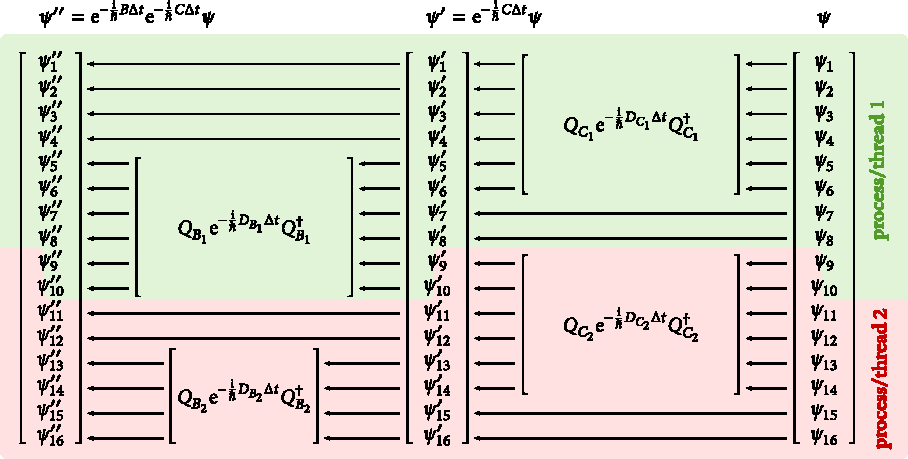
\includegraphics[width=\textwidth]{figures/numerics/parallel_split_step.pdf}
    \caption{Schematic of data flow for parallel split-step method. Computation proceeds right to left. To compute the action of $\ee^{-\frac\ii\hbar B\upDelta t}\ee^{-\frac\ii\hbar C\upDelta t}$ on a vector $\vec\psi$, one can treat the submatrices $B_1$, $B_2$, $C_1$ and $C_2$, of the block-diagonal matrices $B$ and $C$ separately. First, the exponentiation of $C$ can be applied to $\psi$ by applying the exponentiations of $C_1$ and $C_2$ to $\psi$. If diagonalisations $C_1 = Q_{C_1} D_{C_1} Q^\dagger_{C_1}$ and $C_2 = Q_{C_2} D_{C_2} Q^\dagger_{C_2}$ are known, then the two operations can be applied as a series of matrix-vector multiplications and the exponentiation of diagonal matrices. Because the two submatrices are non-overlapping, they can be applied to the vector completely independently in separate computer processes, \textsc{cpu} or \textsc{gpu} threads, or cluster nodes. The exponentiation of $B$ can then be applied to the resulting intermediate vector $\vec\psi^\prime$, similarly via two independent operations acting on nonoverlapping elements of $\psi^\prime$. However, because each submatrix of $C$ overlaps each submatrix of $B$ by $b=2$ elements on either side ($b$ being the bandwidth of the original matrix $A=B+C$), threads/processes must share these elements (here the ninth and tenth elements), sending them to each other whenever they have been updated. For simplicity this example has two compute threads and two submatrices in each term $B$ and $C$, but in general there can be any number of either. When a single thread must apply the exponentiation of multiple submatrices to the state vector, it is advantageous for it to first compute the result of any submatrix whose output is required by another thread, then all submatrices that are independent of other threads, and finally any submatrix which requires input from another thread. In this way, data required by other threads can be sent as early as possible, and data needed from other threads called upon as late as possible, minimising the time that threads are waiting for each other whilst there is useful work to be done.}
    \label{fig:parallel_split_step}
\end{figure}

Whilst this specific banded matrix $A$ is small for the sake of example, in general of course one might have a matrix of any size, allowing for $B$ and $C$ to contain more than two submatrices each. The submatrices have a minimum size of twice the bandwidth $b$ of $A$, in order to cover all elements of $A$ whilst only sharing elements with their nearest neighbour submatrices (any smaller and they would share elements with their next nearest neighbour submatrices as well, complicating things somewhat). But the only maximum is the size of $A$ itself. So what is the optimal submatrix size? Although the split-step method is still accurate to the same order in $\upDelta t$ no matter how many pieces we split a banded matrix into, we clearly introduce additional `commutation error' every time we split $A$ into additional submatrices. So one might think that the number of pieces ought be be minimised, and hence the submatrix size maximised. With regard to this, one might decide to split $A$ into $2n_\up{threads}$ submatrices (where $n_\up{threads}$ is the number of independent computational threads available), half of which will reside in $B$ and half in $C$. This minimises the extra commutation error subject to the constraint that all threads are put to use---splitting $A$ into yet smaller pieces within one computational thread will only yield unnecessary additional error.

Is this the best option? No. Despite the extra commutation error, there is additional benefit to splitting $A$ into more submatrices than required for parallelisation. Let $s$ be the `nominal' size of each submatrix, that is, the size of the corresponding \emph{non-overlapping} submatrices prior to expanding each one along the diagonal (creating overlap) by a number of elements equal to the bandwidth $b$. The computational cost of the matrix-vector multiplications for computing the action of $\ee^{-\frac\ii\hbar B\upDelta t}\ee^{-\frac\ii\hbar C\upDelta t}$ on a vector is then $\Ord{(s+b)^2}$ per submatrix, since $s+b$ is the size of the submatrices in terms of their nominal size and the bandwidth. The total number of submatrices required to cover $A$ is $ns^{-1}$, where $n$ is the size of $A$, and so the total cost of applying the exponentiations of all submatrices to a vector is $\Ord{ns^{-1}(s+b)^2}$. The cost \emph{per unit time} of simulation is then $\Ord{n\upDelta t^{-1}s^{-1}(s+b)^2}$. Here we see that splitting into smaller submatrices is desirable from the point of view of speed: because matrix-vector multiplication runs in quadratic time, a larger number of smaller matrices can be multiplied by vectors faster than a smaller number of larger matrices.

But the more submatrices, the more commutation error. Extra error can be made up for by making the timestep smaller, which increases the cost per unit time once more. So is it worth it? The extra commutation error from splitting up $A$ into more and more pieces in general depends on the form of $A$. I performed a small numerical experiment to see how the commutator $[B, C]$ (which the commutation error is proportional to) scales with $s$ for random banded matrices, as well as those corresponding to 2nd, 4th and 6th order finite differences for first and second derivatives. The result in all cases was that the commutator scaled as $s^{-\frac12}$ (see \figref{fig:commutation_error}).

\begin{figure}[t]
    \centerfloat
    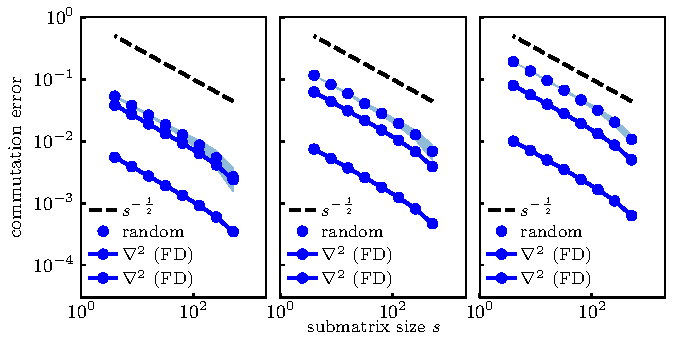
\includegraphics[width=\textwidth]{figures/numerics/commutation_error.pdf}
    \caption{Numerical experiment to determine how the commutation error scales with the submatrix size when splitting certain banded matrices into the sum of block-diagonal matrices and using a split-operator method to exponentiate the sum. From left to right, matrices with bandwidth $b=1$, $b=1$ and $b=2$ are considered. For each bandwidth, the matrices for the finite difference schemes of the order resulting in that bandwidth for first and second derivatives are considered, as well as random matrices of the given bandwidth. The random matrices have real and imaginary parts of each element within the band drawn from standard normal distributions. All matrices are $1024\times1024$. Calculations with random matrices were performed on 20 independent random matrices, and the mean and standard deviation (shaded) of the results plotted. The error metric is the \textsc{rms} element of the commutator $[B, C]$, where the orginal matrix $A$ is split into the sum of block-diagonal matrices $B + C$ using a submatrix size of $s$ (desribed in-text). The \textsc{rms} error in a vector propagated with the split-operator method is proportional this error metric. The result in all cases is that the commutator error, and therefore the error in the split-operator method scales with the submatrix size as $s^{-\frac12}$.}
    \label{fig:commutation_error}
\end{figure}

Back to our question---does decreasing the timestep size $\upDelta t$ to compensate for the additional commutation error result in more, or less computational cost per unit time than if we hadn't split $A$ into more pieces than required for parallelisation? Taking into account the nominal submatrix size $s$ and the method's error in terms of $\upDelta t$, the total error of integrating using the split-step method (assuming the $s^{-\frac12}$ commutator scaling holds) is $\Ord{\upDelta t^a s^{-\frac12}}$, where $a$ is the order in $\upDelta t$ of the accuracy of the specific split-step method used ($1$, $2$, or $4$ for those I've discussed). Using these two pieces of information: the total error, and the total cost per unit time; we can now answer the question ``What value of $s$ minimises the computational cost per unit time, assuming constant error?".

For constant error we set $\upDelta t^a s^{-\frac12} \propto 1$ and get that the computational cost per unit time at constant error is $\Ord{ns^{-\frac1{2a} - 1}(s + b)^2}$. For $a > \frac12$, this expression has a minimum at $s=b$, which is the smallest possible submatrix size in any case. For our example banded matrix $A$, decomposition into the smallest possible submatrices looks like this:
\setlength{\arraycolsep}{1pt}
\begin{align}
& A  = \left[\begin{smallmatrix}
     c & d & e &\mb&\mb&\mb&\mb&\mb&\mb&\mb&\mb&\mb&\mb&\mb&\mb&\mb\\
     b & c & d & e &\mb&\mb&\mb&\mb&\mb&\mb&\mb&\mb&\mb&\mb&\mb&\mb\\
     a & b & c & d & e &\mb&\mb&\mb&\mb&\mb&\mb&\mb&\mb&\mb&\mb&\mb\\
    \mb& a & b & c & d & e &\mb&\mb&\mb&\mb&\mb&\mb&\mb&\mb&\mb&\mb\\
    \mb&\mb& a & b & c & d & e &\mb&\mb&\mb&\mb&\mb&\mb&\mb&\mb&\mb\\
    \mb&\mb&\mb& a & b & c & d & e &\mb&\mb&\mb&\mb&\mb&\mb&\mb&\mb\\
    \mb&\mb&\mb&\mb& a & b & c & d & e &\mb&\mb&\mb&\mb&\mb&\mb&\mb\\
    \mb&\mb&\mb&\mb&\mb& a & b & c & d & e &\mb&\mb&\mb&\mb&\mb&\mb\\
    \mb&\mb&\mb&\mb&\mb&\mb& a & b & c & d & e &\mb&\mb&\mb&\mb&\mb\\
    \mb&\mb&\mb&\mb&\mb&\mb&\mb& a & b & c & d & e &\mb&\mb&\mb&\mb\\
    \mb&\mb&\mb&\mb&\mb&\mb&\mb&\mb& a & b & c & d & e &\mb&\mb&\mb\\
    \mb&\mb&\mb&\mb&\mb&\mb&\mb&\mb&\mb& a & b & c & d & e &\mb&\mb\\
    \mb&\mb&\mb&\mb&\mb&\mb&\mb&\mb&\mb&\mb& a & b & c & d & e &\mb\\
    \mb&\mb&\mb&\mb&\mb&\mb&\mb&\mb&\mb&\mb&\mb& a & b & c & d & e \\
    \mb&\mb&\mb&\mb&\mb&\mb&\mb&\mb&\mb&\mb&\mb&\mb& a & b & c & d \\
    \mb&\mb&\mb&\mb&\mb&\mb&\mb&\mb&\mb&\mb&\mb&\mb&\mb& a & b & c \\
\end{smallmatrix} \right]\nonumber\\
& =\left[ \begin{xsmallmatrix}
     c & d & e &\mb&\mb&\mb&\mb&\mb&\mb&\mb&\mb&\mb&\mb&\mb&\mb&\mb\\
     b & c & d & e &\mb&\mb&\mb&\mb&\mb&\mb&\mb&\mb&\mb&\mb&\mb&\mb\\
     a & b &c/2&d/2&\md&\mb&\mb&\mb&\mb&\mb&\mb&\mb&\mb&\mb&\mb&\mb\\
    \mb& a &b/2&c/2&\md&\md&\mb&\mb&\mb&\mb&\mb&\mb&\mb&\mb&\mb&\mb\\
    \mb&\mb&\md&\md&c/2&d/2& e &\mb&\mb&\mb&\mb&\mb&\mb&\mb&\mb&\mb\\
    \mb&\mb&\mb&\md&b/2&c/2& d & e &\mb&\mb&\mb&\mb&\mb&\mb&\mb&\mb\\
    \mb&\mb&\mb&\mb& a & b &c/2&d/2&\md&\mb&\mb&\mb&\mb&\mb&\mb&\mb\\
    \mb&\mb&\mb&\mb&\mb& a &b/2&c/2&\md&\md&\mb&\mb&\mb&\mb&\mb&\mb\\
    \mb&\mb&\mb&\mb&\mb&\mb&\md&\md&c/2&d/2& e &\mb&\mb&\mb&\mb&\mb\\
    \mb&\mb&\mb&\mb&\mb&\mb&\mb&\md&b/2&c/2& d & e &\mb&\mb&\mb&\mb\\
    \mb&\mb&\mb&\mb&\mb&\mb&\mb&\mb& a & b &c/2&d/2&\md&\mb&\mb&\mb\\
    \mb&\mb&\mb&\mb&\mb&\mb&\mb&\mb&\mb& a &b/2&c/2&\md&\md&\mb&\mb\\
    \mb&\mb&\mb&\mb&\mb&\mb&\mb&\mb&\mb&\mb&\md&\md&c/2&d/2& e &\mb\\
    \mb&\mb&\mb&\mb&\mb&\mb&\mb&\mb&\mb&\mb&\mb&\md&b/2&c/2& d & e \\
    \mb&\mb&\mb&\mb&\mb&\mb&\mb&\mb&\mb&\mb&\mb&\mb& a & b & c & d \\
    \mb&\mb&\mb&\mb&\mb&\mb&\mb&\mb&\mb&\mb&\mb&\mb&\mb& a & b & c \\
\end{xsmallmatrix} \right]
+\left[ \begin{xsmallmatrix}
    \md&\md&\md&\mb&\mb&\mb&\mb&\mb&\mb&\mb&\mb&\mb&\mb&\mb&\mb&\mb\\
    \md&\md&\md&\md&\mb&\mb&\mb&\mb&\mb&\mb&\mb&\mb&\mb&\mb&\mb&\mb\\
    \md&\md&c/2&d/2& e &\mb&\mb&\mb&\mb&\mb&\mb&\mb&\mb&\mb&\mb&\mb\\
    \mb&\md&b/2&c/2& d & e &\mb&\mb&\mb&\mb&\mb&\mb&\mb&\mb&\mb&\mb\\
    \mb&\mb& a & b &c/2&d/2&\md&\mb&\mb&\mb&\mb&\mb&\mb&\mb&\mb&\mb\\
    \mb&\mb&\mb& a &b/2&c/2&\md&\md&\mb&\mb&\mb&\mb&\mb&\mb&\mb&\mb\\
    \mb&\mb&\mb&\mb&\md&\md&c/2&d/2& e &\mb&\mb&\mb&\mb&\mb&\mb&\mb\\
    \mb&\mb&\mb&\mb&\mb&\md&b/2&c/2& d & e &\mb&\mb&\mb&\mb&\mb&\mb\\
    \mb&\mb&\mb&\mb&\mb&\mb& a & b &c/2&d/2&\md&\mb&\mb&\mb&\mb&\mb\\
    \mb&\mb&\mb&\mb&\mb&\mb&\mb& a &b/2&c/2&\md&\md&\mb&\mb&\mb&\mb\\
    \mb&\mb&\mb&\mb&\mb&\mb&\mb&\mb&\md&\md&c/2&d/2& e &\mb&\mb&\mb\\
    \mb&\mb&\mb&\mb&\mb&\mb&\mb&\mb&\mb&\md&b/2&c/2& d & e &\mb&\mb\\
    \mb&\mb&\mb&\mb&\mb&\mb&\mb&\mb&\mb&\mb& a & b &c/2&d/2&\md&\mb\\
    \mb&\mb&\mb&\mb&\mb&\mb&\mb&\mb&\mb&\mb&\mb& a &b/2&c/2&\md&\md\\
    \mb&\mb&\mb&\mb&\mb&\mb&\mb&\mb&\mb&\mb&\mb&\mb&\md&\md&\md&\md\\
    \mb&\mb&\mb&\mb&\mb&\mb&\mb&\mb&\mb&\mb&\mb&\mb&\mb&\md&\md&\md\\
\end{xsmallmatrix} \right].
\end{align}

So the conclusion is: use the smallest submatrices possible when decomposing a banded matrix into a sum of two block-diagonal matrices. The decrease in computational costs, even when the increased error is compensated for by a smaller timestep, is worth it.

\subsubsection{Limitations and nonlinearity}\label{sec:limitations_nonlinearity}

The split-step method is quite powerful and general. It allows you to approximately decompose the exponentiation of a Hamiltonian into exponentiations of its component terms, in the subspaces that they act on, and avoids exponentiating large banded matrices; saving on computing power immensely compared to exponentiating the full Hamiltonian. It is unitary (when the Hamiltonian is actually Hermitian), and stable---that is, unlike Runge--Kutta methods, the method's truncation error does not grow without limit as the simulation proceeds but is bounded (disregarding floating point rounding error, which is much smaller than the truncation error of either method) \cite{schneider_parallel_2006}. This is extremely appealing. And, whilst higher order split-step methods quickly become unwieldy \cite{schneider_parallel_2006}, fourth order accuracy is quite acceptable for many problems.

Applying all the tricks described in the above sections results in $\Ord{\upDelta t}$, $\Ord{\upDelta t^2}$ and $\Ord{\upDelta t^4}$ accurate timestepping methods for solving the Schr\"odinger equation with total computational cost scaling as $\Ord{n \sum_i b_i}$, where $n=\prod_i n_i$ (for a product space of subspaces with dimensionalities $\{n_i\}$) is the dimensionality of the total Hilbert space, and $\{b_i\}$ are the bandwidths of the matrix representations of each term in the Hamiltonian in the chosen basis.\footnote{Now that we are here, we can finally say something about the best basis for simulating in: to minimise computational costs, the best basis is the one that minimises precisely this sum of bandwidths. The exception to this is when fast Fourier transforms are involved, which I discuss later.} Furthermore, the method is efficiently parallelisable, provided the the maximum size-to-bandwidth ratio $\max_i(n_i/b_i)$ of the terms in the Hamiltonian is much larger than the number of parallel computing threads available. Although the constant factors that big-O notation neglects may not be optimal, this scaling would seem to be the best one could hope for---for each of the $n$ elements in the state vector one must consider the $\sum_i b_i$ elements (including itself) that the Hamiltonian couples it with, and no more.\footnote{Assuming the banded matrices are otherwise dense within their band---further improvements would be possible if some elements within the band were always zero.}

The main downside of this otherwise excellent method of exponentiating Hamiltonians is that the evolution modelled must actually be described by a linear system of equations. One cannot add arbitrary terms and nonlinear operators to the Hamiltonian, as the split-step method requires that one can evaluate each time-dependent term in the Hamiltonian at specific times, including times at which the solution for the state vector is not yet available. This would seem to limit the split-step method strictly to modelling \emph{linear} dynamics, that is, terms in the Hamiltonian must not depend explicitly on the state vector they are operating on. Whilst nature might fundamentally be described by linear dynamics, once approximations of various kinds are made in order to make problems tractable, it's common to end up with a nonlinear pseudopotential or nonlinear effective Hamiltonian. Note that non-\emph{Hermitian}, pseudo-Hamiltonians---leading to non-unitary evolution---are fine. The split-step method has made no assumptions that rules them out, it only assumes the differential equation can be expressed in the form
\begin{align}
\dv t \vec\psi(t) = \sum_n H_n(t)\vec\psi(t),
\end{align}
where $\{H_n\}$ are a set of linear operators, Hermitian or not.

Fortunately, one specific form of nonlinearity that cold atom physicists are particularly interested in---the nonlinear term in the Gross--Pitaevskii equation---can be incorporated without much difficulty. As mentioned, the problem with nonlinearity is that all but the first-order split step methods require you to evaluate terms in the Hamiltonian at some future time at which the state vector is not yet known, that is the algorithm contains steps akin to $\vec \psi(t_{n+1}) = U(t_{n+1}, t_n; \vec\psi(t_{n+1})) \vec \psi(t_n)$ for some nonlinear unitary matrix $U(t_{n+1}, t_n; \vec\psi(t_{n+1}))$---$U$ cannot be explicitly constructed because it both requires and is required by $\psi(t_{n+1})$.

For the Gross--Pitaevskii effective Hamiltonian, the second-order split-step method (from which the fourth order method is constructed) for a single step might be na\"ively written
\begin{align}
\vec \psi(t_{n+1}) =
\ee^{-\frac\ii\hbar K \frac{\upDelta t} 2}
\ee^{-\frac\ii\hbar (g\rho(t_{n+1}) + V(t_{n+1})) \frac{\upDelta t} 2}
\ee^{-\frac\ii\hbar (g\rho(t_n) + V(t_n) ) \frac{\upDelta t} 2}
\ee^{-\frac\ii\hbar K \frac{\upDelta t} 2}
\vec \psi(t_n),
\end{align}
where $\vec\psi(t)$ is the state vector\footnote{Usually when modelling the GPE the single-particle state vector is normalised to the number of particles, rather than unity, and so strictly speaking it cannot be called a state vector, though it otherwise can be treated as one in most respects.} represented in a discrete position basis, $g$ is the nonlinear interaction constant, $V(t)$ and $\rho(t) = \vec\psi(t)\vec\psi^\dagger(t)$ are diagonal matrices for the external potential and the density matrix for $\vec\psi(t)$ in the same position basis, and $K$ is a discrete approximation to the kinetic energy operator in the position basis.

As written, this can't be evaluated because $\vec \psi(t_{n+1})$---required to evaluate $\rho(t_{n+1})$---is not yet known. The order we choose to exponentiate the terms in our Hamiltonian is arbitrary, however (so long as we alternately reverse that order each half-step as required by the second order split-step method),
and so swapping the order gives
\begin{align}
\vec \psi(t_{n+1}) =
\ee^{-\frac\ii\hbar (g\rho(t_{n+1}) + V(t_{n+1})) \frac{\upDelta t} 2}
\ee^{-\frac\ii\hbar K \upDelta t}
\ee^{-\frac\ii\hbar (g\rho(t_n) + V(t_n) ) \frac{\upDelta t} 2}
\vec \psi(t_n),
\end{align}
which incidentally has the benefit that since $K$ is (ordinarily) time independent, the two adjacent exponentials containing it can be combined into one. Now $\rho(t_{n+1})$ is contained within the leftmost exponential, and so it is the last operator to be applied in the timestep. Note that since $g\rho(t)$ is real and diagonal in the position basis (as is $V(t)$), this leftmost unitary merely changes the phase of the state vector at each point in space, having no effect on its density. This means that $\rho(t)$ is, in fact, unaffected by this last unitary evolution operator. Hence, $\rho(t_{n+1})$ can be computed simply as the density matrix of the intermediate state vector that this unitary was to act on:
\begin{align}
\rho(t_{n+1}) = \vec\psi(t_{n+1})\vec\psi^\dagger(t_{n+1}) = \tilde{\vec\psi}\tilde{\vec\psi}^\dagger,
\end{align}
where
\begin{align}
\tilde{\vec\psi} = 
\ee^{-\frac\ii\hbar K \upDelta t}
\ee^{-\frac\ii\hbar (g\rho(t_n) + V(t_n) ) \frac{\upDelta t} 2}
\vec \psi(t_n).
\end{align}

The inclusion of $V(t)$ with $g\rho(t)$ is optional, and if $V(t)$ was not real valued, would not be valid (since in that case the density \emph{would} be affected by the evolution induced by $V(t)$). In such a case the Hamiltonian would have to be split into three terms with $V(t)$ and $g\rho(t)$ treated separately.

So now we can put some conditions on what types of nonlinear operators can be used within the second-order split step method. The first condition is that at most one nonlinear operator can be included, since it must be placed last in the sandwich of exponentials (otherwise its value at the end of the timsestep cannot be inferred immediately prior to acting on the state vector). The second condition is that the nonlinear operator must be invariant with respect to the evolution that it itself induces in the state vector. Here we have an operator that  depends only on the state vector's absolute value, but for which the corresponding unitary only evolves the state vector's phase. Another example might be an operator that depends only on the state vector's phase gradients, but evolves the state vector's absolute value, and so forth.

Although I find this argument compelling for second-order split-step, it's less obvious that it should hold for fourth-order split-step as well, which, even though it is based on multiple applications of second-order split-step, involves a substep that is backwards in time. `Evaluate the nonlinear operator based on the state vector at this specific time' becomes ambiguous when that moment in time is traversed in both directions by two different sub-steps. However, \cite{javanainen_symbolic_2006} have verified using computer symbolic algebra that indeed, up to even higher order split-step methods, putting the nonlinear density term last in the splitting and always evaluating it using the value of the intermediate state vector immediately prior results in the method having the same order accuracy in $\upDelta t$ as for linear operators only. Given this and my argument above, as well as the reasoning that the second-order split-step method has no way of `knowing' whether it is acting backward in time or not when embedded in a higher-order split step method, I would expect the same to hold for all nonlinear operators meeting the above two conditions, though I haven't shown this explicitly.

\section{For everything else, there's fourth-order Runge--Kutta}\label{sec:rk4}

Fourth-order Runge--Kutta (\textsc{rk4}) is the enduring workhorse of numerical integration methods. Of the Runge--Kutta methods, it offers a good balance of accuracy and computational cost. When a problem does not have the properties that allow manifestly unitary or error-bounded methods to be used, or when enough computing power can be deployed so as to make these concerns irrelevant, and the programmer's time more important, fourth order Runge--Kutta is a good choice. It downsides are that it is not manifestly unitary, and its error is not bounded. Nonetheless for many problems this is not a concern in practice.

The advantages of fourth-order Runge--Kutta are compelling: it has global error that is fourth order in the integration timestep, involves four function evaluations per timestep, requires only linear arithmetic operations outside of the function evaluations, and can be applied any problem that can be written in the form
\begin{align}
\dv t \vec x = f(\vec x, t),
\end{align}
for some (possibly nonlinear) function $f$, where $\vec{x}$ is a vector of dynamical variables, often in our case the components of a state vector, or for classical dynamics the positions and velocities of an ensemble of particles\footnote{For classical particle dynamics, often lower order symplectic methods such as the leapfrog method \cite{Skeel97afamily} can be preferable, but nonetheless it is hard to overstate the usefulness of a general purpose algorithm such as \textsc{rk4} that can be deployed as a first attempt, or as a plan B once the assumptions required by another algorithm are violated}. Note that this formulation allows for initial value problems with coupled \textsc{ode}s, discretised \textsc{pde}s, as well as second or higher order differential equations, since an equation of the form
\begin{align}
\dv[2] t \vec x = f(\vec x, t)
\end{align}
can be rewritten
\begin{align}
\dv t \left(\vec x, \dot{\vec x}\right) = \left(\dot{\vec x}, f(\vec x, \dot{\vec x}, t)\right),
\end{align}
treating the time derivative of each element of $\vec x$ as simply another coupled dynamical variable.

Not unrelated to its ease of implementation, the method itself can be stated concisely. Propagation of the dynamical variables for one timestep from time $t$ to time $t + \upDelta t$ is computed as follows:
\begin{align}
\vec k_1 &= f(\vec x(t), t),\nonumber\\
\vec k_2 &= f(\vec x(t) + \tfrac12 \vec k_1\upDelta t, t + \tfrac12\upDelta t),\nonumber\\
\vec k_3 &= f(\vec x(t) + \tfrac12 \vec k_2\upDelta t, t + \tfrac12\upDelta t),\nonumber\\
\vec k_4 &= f(\vec x(t) + \vec k_3\upDelta t, t + \upDelta t),\nonumber\\
\vec x(t + \upDelta t) &= \vec x(t)
+ \tfrac{\upDelta t}6(\vec k_1 + 2\vec k_2 + 2\vec k_3 + \vec k_4).\label{eq:rk4}
\end{align}

Each step is self-contained, that is, the algorithm does not contain any state from previous steps. This is appealing as it means that $f$ can change discontinuously between timesteps without giving rise to Runge's phenomenon \cite{dahlquist2003numerical} in the approximate solutions $\vec x(t)$, as can be the case with multistep methods which do retain some dependency on previous steps.
$\vec x(t)$ can also be modified discontinuously between steps without causing problems, as is required by Monte Carlo wavefunction or quantum jump methods \cite{molmer_monte_1996, plenio_quantum-jump_1998}, or even in the imaginary time evolution method (see section \ref{sec:ITEM}) which may require normalisation of the state vector in between steps. Fourth order Runge--Kutta is therefore quite compatible with stochastic processes and many other models which may not be described by a differential equation alone.

One downside is that the timestep used must be much smaller than the timescale on which $\vec x$ changes - even if $\vec x$'s time variation is highly regular. If $\vec x$'s time variation is dominated by the simple accumulation of complex phase at some angular frequency---as is often the case in quantum mechanics---the timesteps used for \textsc{rk4} must be small enough to resolve these circles about the complex plane. This is in contrast to the exponentiation methods, for which an energy offset (and hence overall change in the angular frequency at which the state vector's elements accumulate phase) is largely irrelevant. Energy offsets or use of an interaction picture can mitigate this problem but requires some foresight, and may not be possible if the required energy offsets change in time or are not known analytically in advance. The method I develop in section \ref{sec:rk4ilip} is a partial remedy for this specific problem, which in my opinion is the biggest weakness of fourth order Runge--Kutta as applied to quantum state evolution, when compared to the unitary methods.

\subsection{Complexity and parallelisability for the Schr\"odinger equation}

Excluding the evaluation of $f$, \textsc{rk4} requires a number of arithmetic operations proportional to the number of elements in $\vec x$, and so contributes time-complexity $\Ord{n}$ to the overall calculation, where $n$ is the number of elements in $\vec x$. Since $f$ itself usually doesn't run in linear time, the computational time complexity of \textsc{rk4} is usually therefore that of evaluating $f$. Its parallelisability also comes down to that of $f$, since equations (\ref{eq:rk4}) above treat each element of $\vec x$ completely independently, with any couplings computed within $f$.

For the Schr\"odinger equation in a concrete basis, $f$ is
\begin{align}
f(\vec \psi, t) = -\frac\ii\hbar H(t)\vec \psi,
\end{align}
where $\vec \psi$ is the state vector in the given basis and $H(t)$ is the matrix representation of the Hamiltonian in that basis\footnote{For the Gross--Pitaevskii equation this would be a nonlinear $H(\vec \psi, t)$, and everything else in this section still applies.}. Fourth order Runge--Kutta is therefore as computationally expensive and parallelisable as computing the matrix-vector product $H(t)\vec\psi$. In the worst case this multiplication is $\Ord{n^2}$ in the size of the Hilbert space and barely parallelisable at all, if $H$ is dense. But in the common case (as mentioned in section \ref{sec:split-step}), of $H$ being a sum of terms which act on different subspaces, i.e.
\begin{align}
H(t) = \sum_{i=1}^N \mathbb{I}_{n_1} \otimes \cdots  \otimes \mathbb{I}_{n_{i-1}}
\otimes  H_i(t) \otimes  
 \mathbb{I}_{n_{i+1}} \otimes \cdots \otimes \mathbb{I}_{n_N}
\end{align}
where $n_i$ is the dimensionality of the subspace acted on by the $i^\up{th}$ term and $\mathbb{I}_m$ is the $m\times m$ identity matrix, then things are much better. If each term is dense, then the overall cost of evaluating the product $H(t)\vec\psi$ is $\Ord{n\sum_i n_i}$, where $n = \prod_i n_i$ is the dimensionality of the total Hilbert space, which can be considerably less than the $\Ord{n^2}$ of evaluating the single  matrix-vector product for the total Hamiltonian. And if each term is a banded matrix with bandwidth $b_i$, then the cost of applying a single term in the Hamiltonian becomes $\Ord{n b_i}$ instead of $\Ord{n n_i}$, and so the cost of evaluating $H(t)\vec\psi$ becomes $\Ord{n\sum_i b_i}$. This is identical to the earlier result for the split-operator method once the trick of splitting up banded matrices into block-diagonal matrices was applied (section \ref{sec:split-step-parallel}), but with much less work (in the sense of programmer effort rather than computational complexity). Representing $H(t)$ as a sum of terms over different subspaces is no extra work---this is the form we are likely to be writing Hamiltonians in already, and constructing the total $H(t)$ is often not required if one desires only to propagate a state vector in time.\footnote{Though constructing the matrix form of say, $\frac {\hat p_x^2} {2m} + \frac {\hat p_y^2} {2m}$ for some finite difference or pseudospectral representations of $\hat p_x$ and $\hat p_y$ can be useful if one wants to say, compute the dispersion relation of a particular system by diagonalising it.} No, we are already applying these operators to different subspaces of the Hilbert space and then summing the results without thinking twice about it, and so the above analysis mostly serves as a reminder that what we are already doing most of the time is in fact very efficient. 

Parallelisation, provided one or more of the matrices are banded, is also straightforward, since if $A$ is banded with bandwidth $b$, then
\begin{align}
(A \vec \psi)_i = \sum_{j=-b}^b A_{i, i+j} \psi_j,
\end{align}
that is, calculation of an element of $A\vec\psi$ requires only the corresponding element of $\vec \psi$ and its nearest $b$ neighbours on each side. One can therefore divide up the state vector into contiguous regions (in the subspace in which $A$ acts), and compute different elements of the product on different compute threads, requiring an exchange of only $b$ elements at each boundary\footnote{A note about minimising the effect of latency: at the start of an \textsc{rk4} substep, have each thread send the required elements at the edges of its region in each subspace to its neighbouring threads \emph{first}. \emph{Then} compute $H(t)\vec\psi$ on the interior elements. If each thread has a sufficiently large workload, then by the time this is complete, the data from neighbouring regions will have arrived and threads will not have spent any time waiting for each other.} between neighbouring threads. An example of this is to split two dimensional space into into a number of pieces in each dimension (resulting in a 2\textsc{d} grid) so as to compute the application of (finite difference approximations to) the $x$ and $y$ second derivative operators on a state vector in parallel.

An additional benefit of parallelised \textsc{rk4} when compared to split-operator is that the same amount of data needs to be sent between threads regardless of the number of terms in the Hamiltonian. In split-step methods, each term in the Hamiltonian is exponentiated separately (multiple times for the higher order schemes), requiring an exchange of data each time. The amount of data needing to be exchanged per step therefore scales with the number of terms in the Hamiltonian being parallelised, whereas for \textsc{rk4} it is constant.

The constant factors that big-O notation disregards also favour \textsc{rk4} when compared to split-operator methods. For one, addition and multiplication are much cheaper than exponentiation, meaning that the exponentials in split-operator methods may add considerable computational cost if the Hamiltonian itself is simple. Furthermore, parallelised or not, each term in fourth order split-operator adds $20$ matrix-vector products in the space the term acts, whereas \textsc{rk4} requires only one additional matrix-vector product per term. In practice due to these properties, \textsc{rk4} runs considerably faster than split-operator methods, even for simple systems, and the gap widens as complexity increases.

\subsection{The interaction picture}\label{sec:interaction_picture}

[TODO]

%         \begin{itemize}
%             \item Sometimes called a "rotating frame"
%             \item Is equivalent to basis change where new basis functions differ by a time-dependent phase factor
%             \item Is defined by a time-independent Hamiltonian
%             \item This has the effect of moving some time dependence into the operators (demonstrate, by writing some operators with the unitary in front of them. As you can see it is simply a change of basis - but a time-dependent one.)
%             \item No need to remain in the same interaction picture - can be redefined arbitrarily often throughout a simulation and state vectors transformed into new basis.
%         \end{itemize}
% \begin{itemize}

% \item {absorbing boundary conditions, reflective boundary conditions, periodic boundary conditions}

% \end{itemize}

\section{Continuous degrees of freedom}\label{sec:continuous_dof}
The single-particle, non-relativistic, scalar Schr\"odinger wave equation, as distinct from the general Schr\"odinger equation \eqref{eq:schrodinger_equation}, is:
\begin{align}\label{eq:schrodinger_wave_equation}
\ii\hbar\pdv{}{t}\psi(\vec r, t) = \left[-\frac{\hbar^2}{2m} \nabla^2 + V(\vec r)\right]\psi(\vec r, t).
\end{align}
Similarly, as mentioned in [SECREF INTRODUCTION], the equation for the single-particle wavefunction of an atom in a single-component Bose--Einstein condensate is the Gross--Pitaevskii equation
\begin{align}
\ii\hbar\pdv{}{t}\psi(\vec r, t) = \left[-\frac{\hbar^2}{2m} \nabla^2 + V(\vec r) + g\abs{\psi(\vec r, t)}^2\right]\psi(\vec r, t),
\end{align}
where $\psi(\vec r, t) = \sqrt{N}\braket{\vec r}{\psi(t)}$ is the single-particle wavefunction scaled by the square root number of atoms $N$.

Both these equations are partial differential equations involving both spatial and temporal derivatives. But in numerical quantum mechanics all state vectors are mapped to column vectors and all operators to matrices. Spatial wavefunctions are no exception to the former and differential operators such as $\grad^2$ are no exception to the latter--these objects can be thought of as infinite-dimensional vectors and matrices. So the above two equations are specific instances of the general Schr\"odinger equation \eqref{eq:schrodinger_equation}, given specific Hamiltonians, and represented in a concrete---albeit infinite-dimensional---basis. But we can only perform a finite number of computations, so what do these vectors and operators look like once we reduce them to something finite? That depends on whether we choose to discretise space on a grid, or use a functional basis (and on which functional basis we choose). As we'll see, however, spatial discretisation can be a special case of a functional basis, namely the Fourier basis, plus an additional approximation or two. The resulting matrices are \emph{banded}, justifying the previous two sections' attention to dealing with banded matrices efficiently.

\subsection{Spatial discretisation on a uniform grid: the Fourier basis}

Imagine a two dimensional spatial region within which we are solving the single-component Gross--Pitaevskii equation, evolving an initial condensate wavefunction in time. Having specified which degrees of freedom we want to simulate (two continuous degrees of freedom, one for each spatial dimension), the next step according to the method outlined in section \ref{sec:neglect_discretisation} is to choose a basis in which to represent this state vector.

Let's say we discretise space in an equally-spaced $n_x\times n_y = 7\times 7$ rectangular grid,\footnote{For the sake of example---$256\times256$ is a more realistic minimum.} with spacings $\upDelta x$ and $\upDelta y$, and only represent the wavefunction at those $49$ points in space. The state vector can then be represented by a list of $49$ complex numbers, each taken to be the wavefunction's value at the spatial position corresponding to one gridpoint. This $49$-vector is now a concrete representation of our state vector (\figref{fig:vector_unravel}).

\begin{figure}[t]
    \centerfloat
    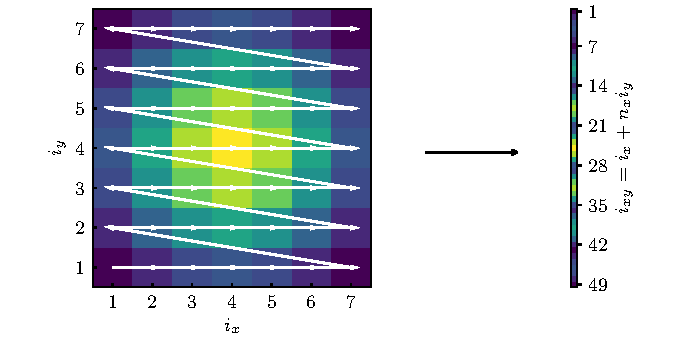
\includegraphics[width=\textwidth]{figures/numerics/vector_unravel.pdf}
    \caption{Discretising a function over two dimensional space on a grid yields a list of coefficients, one for each gridpoint. These can be arranged as a column vector, and in this way a two dimensional wavefunction approximated by a finite-dimensional state vector. Computationally we don't normally treat this state vector as a column vector---it is more convenient to leave it as a two-dimensional array. But conceptually it is a single vector living in the product space of the discretised $x$ and $y$ spaces.}
    \label{fig:vector_unravel}
\end{figure}

\begin{figure}[t]
    \centerfloat
    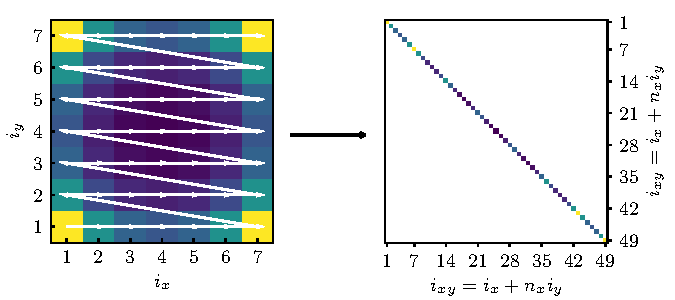
\includegraphics[width=\textwidth]{figures/numerics/potential_unravel.pdf}
    \caption{A discretised potential energy operator can be formed by evaluating the function for the potential at a set of gridpoints. The resulting matrix is diagonal and square with $n_x \times n_y$ rows and columns. Since multiplying this operator by a state vector entails multiplying each element of the state vector by one diagonal element of the potential operator, both the state vector and the diagonals of the potential operator can be stored in simulation code as 2\textsc{d} arrays and multiplied elementwise, hiding somewhat the fact that the operation is still a matrix-vector product. This way of discretising a potential operator is called the pseudospectral approximation, and is described later in this section}
    \label{fig:potential_unravel}
\end{figure}

We can also evaluate the potential (and nonlinear term in the case of the Gross--Pitaevskii equation) at each gridpoint and declare this a diagonal operator (\figref{fig:potential_unravel}). Finally, we could use finite differences to compute the Laplacian - equivalent to replacing the Laplacian with a matrix
\begin{align}
L = L_x \otimes \mathbb{I}_{n_y} + \mathbb{I}_{n_x} \otimes L_y 
\end{align} 
where $L_x$ and $L_y$ are (banded) matrices for finite-difference approximations to second derivatives in each direction. We might also use discrete Fourier transforms to evaluate the Laplacian, since
\begin{align}
\nabla^2\psi(\vec r) = \mathcal{F}^{-1}\left\{-k^2\mathcal{F}\{\psi(\vec r)\}(\vec k)\right\},
\end{align}
where $ k = \abs{\vec k}$.

This is all well and good, and it works. But at what point did we choose a basis just now---what are the basis vectors? This just looks like discretising space at a certain resolution, rather than the formal process of choosing a basis and projecting the state vector and operators onto each basis vector, as outlined in section \ref{sec:neglect_discretisation}. Assuming what we've done is equivalent to choosing a basis, that basis has a finite number ($49$) of basis vectors, which means it cannot be complete, since state vectors we're approximately representing with it require an infinite number of complex numbers to be described exactly.\footnote{One for each position within the two dimensional space we're representing.} So what do the basis functions look like, and what state vectors have we implicitly excluded from simulation by choosing a basis that is incomplete?

Prior to discretisation, the spatial wavefunction $\psi(\vec r, t) = \braket{\vec r}{\psi(t)}$ was already the representation of the abstract state vector $\ket{\psi}$ in the ``spatial basis"---a basis in which the basis vectors $\{\ket{\vec r}\}$ are Dirac deltas positioned at each point in space. The value of the wavefunction $\psi(\vec r)$ for a specific $\vec r$ is then simply a coefficient saying how much of the basis vector $\ket{\vec r}$ to include in the overall state vector. What we have \emph{not} done is chosen a subset of these Dirac delta basis functions as our basis. This would be very strange---our representation of the wavefunction would allow it to be nonzero at the gridpoints, but not in between, like a comb. Spatially separated Dirac deltas do not spatially overlap at all; the matrix elements of the kinetic energy operator:
\begin{align}
\matrixel{\vec r_i}{\hat K}{\vec r_j} = \int \delta(\vec r - \vec r_i)\left(-\frac{\hbar^2}{2m}\grad^2\right)\delta(\vec r - \vec r_j)\,\dd \vec r
\end{align}
would all be zero for $i\neq j$, disallowing any flow of amplitude from one point in space to another by virtue of it not being able to pass through the intervening points.

Neither have we implicitly chosen a set of two-dimensional boxcar functions centred on each gridpoint with width $\upDelta x$ and $\upDelta y$ in each direction respectively. These cover all space in between gridpoints, but are are not twice differentiable everywhere, and hence the kinetic energy operator's matrix elements cannot be evaluated\footnote{Delta functions aren't twice differentiable either, so this itself isn't a fatal flaw--but even if one defines the boxcar functions as the limit of twice differentiable functions becoming increasingly square with some parameter, the limit for the kinetic energy matrix elements between adjacent boxcars goes to infinity.}. No, neither of these bases makes sense. To interpret our spatial grid as a basis, we need a set of functions $\phi_{ij}(r)$ (where $i$ and $j$ are the indices of the gridpoints in the $x$ and $y$ directions respectively) that are orthonormal, are nonzero only at one gridpoint and are zero at all others, and are twice differentiable everywhere in our spatial region. Infinite choices are available, differing in which subspace of the original Hilbert space they cover. A sensible heuristic for choosing one is that we want to be able to represent the state vectors whose wavefunctions do not change much between adjacent gridpoints, and we are happy for the necessary incompleteness of our basis to exclude wavefunctions with any sort of structure in between gridpoints.

\subsubsection{The discrete Fourier transform to the rescue}

It turns out that discretising space in this way can indeed be equivalent to choosing a sensible basis. This is made clearer by first discretising in Fourier space instead, and seeing how this can imply a discretisation in real space.

One possible basis for representing all possible state vectors is the Fourier basis $\{\ket{\vec k_{ij}}\}$. With it, any state vector (whose wavefunction is nonzero only within the \textsc{2d} region) can be represented as the sum of basis vectors whose wavefunctions are \textsc{2d} plane waves, also localised to the 2\textsc{d} region:
\begin{align}\label{eq:spatial_plane_wave_basis}
\braket{\vec r}{\vec k_{ij}} = \begin{cases}
\frac 1 {\sqrt A} e^{i\vec k_{ij}\cdot\vec r}\qquad (\vec r\ \textrm{within \textsc{2d} region})\\
0\qquad(\vec r\ \textrm{not within \textsc{2d} region}),
\end{cases}
\end{align}
where $A$ is the area of the \textsc{2d} region and the wavevector of each plane wave is
\begin{align}
\vec k_{ij} = \left[ \tfrac {2\pi i}{L_x}, \tfrac {2\pi j}{L_y}\right]^\up{T},
\end{align}
where $i$ and $j$ are (possibly negative) integers. Any state vector whose wavefunction is localised to the \textsc{2d} region can then be written as the infinite sum:
\begin{align}
\ket\psi &= \sum_{i=0}^\infty\sum_{j=0}^\infty \braket{\vec k_{i,j}}\psi \ket{\vec k_{i,j}}\\
\Rightarrow \psi(\vec r) &= \braket{\vec r}{\psi} = \begin{cases}
\sum_{i=0}^\infty\sum_{j=0}^\infty \braket{\vec k_{ij}}\psi \frac 1 {\sqrt A} e^{i\vec k_{ij}\cdot\vec r}
\qquad (\vec r\ \textrm{within \textsc{2d} region})\\
0\qquad(\vec r\ \textrm{not within \textsc{2d} region}).
\end{cases}
\end{align}
So $\{\braket{\vec k_{ij}}\psi\}$ are simply the coefficients of the \textsc{2d} Fourier series of $\psi(\vec r)$.

What does this have to do with our discretised space? These basis functions $\{\braket{\vec r}{\vec k_{ij}}\}$ don't have the required properties for a spatial discrete basis. For one, there are an infinite number of them, and we require 49 for our 7$\times$7 example. Secondly, all of them are nonzero everywhere within the \textsc{2d} region, whereas we require each basis function to be nonzero at exactly one of our 49 gridpoints.

We can solve the first problem by truncating the Fourier series. By only including basis vectors $\ket{\vec k_{ij}}$ for which:
\begin{align}
\begin{cases}
i \in [-\tfrac{n_x}2, \tfrac{n_x}2 - 1] \qquad (n_x\ \textrm{even})\\
i \in [-\tfrac{n_x - 1}2, \tfrac{n_x - 1}2] \qquad (n_x\ \textrm{odd})
\end{cases}
\end{align}
and
\begin{align}
\begin{cases}
j \in [-\tfrac{n_y}2, \tfrac{n_y}2 - 1] \qquad (n_y\ \textrm{even})\\
j \in [-\tfrac{n_y - 1}2, \tfrac{n_y - 1}2] \qquad (n_y\ \textrm{odd})
\end{cases}
\end{align}
we include only the $n_x$ and $n_y$ longest wavelengths in each respective spatial dimension. This is a sensible truncation with a physically meaningful interpretation. By making it, we are no longer able to represent state vectors with short wavelength components. Because the kinetic energy operator, when represented in the Fourier basis, is:
\begin{align}
\matrixel{\vec k_{ij}}{\hat K}{\vec k_{i^\prime j^\prime}} = \frac{\hbar^2 k^2}{2m}\updelta_{ii^\prime}\updelta_{jj^\prime},
\end{align}
where $k = |\vec k_{ij}|$, by excluding basis vectors with larger wavevectors, we are excluding state vectors with large kinetic energy. Thus the truncation is a kinetic energy cutoff, and is an accurate approximation whenever a simulation is such that the system is unlikely to obtain kinetic energies above the cutoff.\footnote{Because a \emph{square} region in Fourier space is being carved out, by limiting each of $k_x$ and $k_y$ to finite ranges rather than the total wavenumber $k = \sqrt{k_x^2 + k_y^2}$, there is no single kinetic energy cutoff so to speak. Nonetheless there is a maximum wavenumber $k_\up{max} = \min(\{|k_x|\} \cup \{|k_y|\})$ defining a kinetic energy cutoff $K_\up{max} = \hbar^2k_\up{max}^2/(2m)$ below which kinetic energies definitely are representable and above which they may not be.} It also matches our earlier intuition that our basis should represent wavefunctions that don't vary much between gridpoints---here we are discarding short wavelengths and hence limiting wavefunctions we can represent to ones that vary slowly in space compared to the cutoff wavelength.

Now we have a set of basis vectors---a discrete Fourier basis---but their spatial wavefunctions still don't have the property of being nonzero only at a single gridpoint each. On the contrary, each plane wave has has a constant amplitude everywhere in space. But consider the following superposition of Fourier basis vectors:
\begin{align}\label{eq:DFT_basischange}
\ket{\vec r_{ij}} = \sum_{i^\prime}\sum_{j^\prime} e^{-i \vec k_{i^\prime j^\prime} \cdot \vec r_{i j}}\ket{\vec k_{i^\prime j^\prime}}
\end{align}

with $\vec r_{i j} = (i \upDelta x, j \upDelta y)^\up{T}$. The set of vectors $\{\ket{\vec r_{i, j}}\}$ are also an orthonormal basis, related to the discrete Fourier basis by a unitary transformation with matrix elements:
\begin{align}
U_{\textsc{dft2}, i^\prime j^\prime ij} = \braket{\vec k_{i^\prime j^\prime}}{\vec r_{i j}} = e^{-i \vec k_{i^\prime j^\prime} \cdot \vec r_{i j}}.
\end{align}

This unitary transformation is in fact a two-dimensional discrete Fourier transform (hence the subscript), and the basis vectors $\{\ket{\vec r_{ij}}\}$ have spatially localised wavefunctions that are nonzero only at one of the spatial gridpoints. Vectors and matrices can be transformed from their discrete Fourier space representation to their discrete real-space representation and back using the unitary $U_{\textsc{dft2}}$:

\begin{align}
\vec\psi_\up{real} &= U^\dagger_{\textsc{dft2}} \vec \psi_\up{Fourier}\\
\vec\psi_\up{Fourier} &= U_{\textsc{dft2}} \vec \psi_\up{real}\\
A_\up{real} &= U^\dagger_{\textsc{dft2}} A_\up{Fourier} U_{\textsc{dft2}}\\
A_\up{Fourier} &= U_{\textsc{dft2}} A_\up{Real} U^\dagger_{\textsc{dft2}}.
\end{align}
where $\vec\psi_\up{real}$ is the vector of coefficients $\psi_{\up{real},ij}= \braket{\vec r_{ij}}{\psi}$ for representing a state vector in the discrete real space basis, $\vec\psi_\up{Fourier}$ is the vector of coefficients $\psi_{\up{Fourier}, ij} = \braket{\vec k_{ij}}{\psi}$ for the state vector in the discrete Fourier basis, and $A_\up{real}$ and $A_\up{Fourier}$ are the representations of some operator $\hat A$ in the discrete real and Fourier bases respectively, with matrix elements $A_{\up{real}, ij i^\prime j^\prime} = \matrixel{\vec r_{ij}}{\hat A}{\vec r_{i^\prime j^\prime}}$ and $A_{\up{Fourier},ij i^\prime j^\prime} = \matrixel{\vec k_{ij}}{\hat A}{\vec k_{i^\prime j^\prime}}$.

\begin{figure}[t]
    \centerfloat
    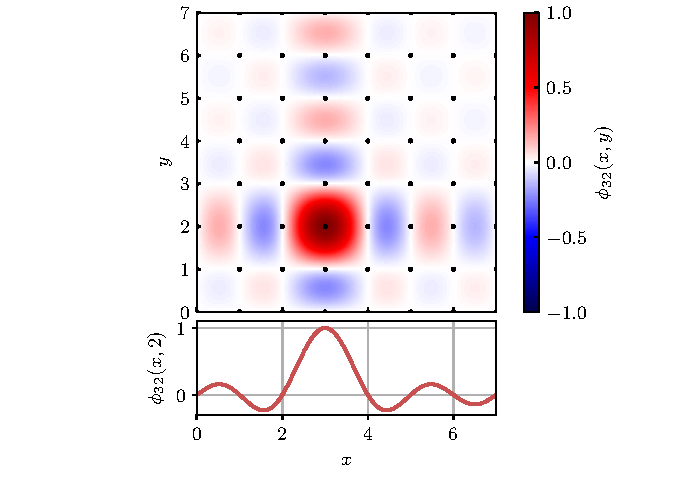
\includegraphics[width=\textwidth]{figures/numerics/basis_vecs.pdf}
    \caption{An example of the spatial representation of one of the basis vectors obtained by transforming the discrete Fourier basis using the discrete Fourier transform. Since the discrete Fourier transform is a unitary transformation, the set of these basis functions forms an equivalent orthonormal basis for representing state vectors and operators.}

    \label{fig:basis_vecs}
\end{figure}

The spatial representation of the basis vectors $\{\ket{\vec r_{ij}}\}$ can be computed using \eqref{eq:spatial_plane_wave_basis} as:
\begin{align}
\phi_{ij}(\vec r) &= \braket{\vec r}{\vec r_{i j}} = \sum_{i^\prime j^\prime} e^{-\ii \vec k_{i^\prime j^\prime} \cdot \vec r_{i j}}\braket{\vec r}{\vec k_{i^\prime j^\prime}}\\
\Rightarrow \phi_{ij}(\vec r) &=\begin{cases}
\sum_{i^\prime j^\prime} \frac 1 {\sqrt {L_x L_y}} e^{\ii \vec k_{i^\prime j^\prime} \cdot (\vec r - \vec r_{i j})}\qquad (\vec r\ \textrm{within \textsc{2d} region})\\
0\qquad(\vec r\ \textrm{not within \textsc{2d} region}),
\end{cases}
\end{align}
where $L_x$ and $L_y$ are the spatial extents of the $x$ and $y$ dimensions. An example of one of these basis vectors in the spatial representation is plotted in \figref{fig:basis_vecs}.

These functions are sometimes called \emph{periodic sinc functions}, \emph{band-limited delta functions}, or the \emph{Dirichlet kernel}
\citeleft\citen{bruckner1997real}, p.~619; \citen{levi_geometric_1974}\citeright.
Each of them is zero at all of the gridpoints except one, and and they form an orthonormal basis set. They satisfy all of our requirements to be a basis corresponding to our gridded discretisation of space.

One thing to note is that these functions are periodic. By using the Fourier basis in the way we have to restrict our basis to cover only a finite region of both Fourier space and real space, we have necessarily imposed periodicity on the problem. This periodicity shows itself when we compute matrix elements of operators in this basis - if we compute the kinetic energy operator's matrix elements for example, it will couple basis states across the boundary of the region, resulting in spatial periodicity---a wavepacket moving rightward through the right boundary will emerge moving rightward from the left boundary.

Less obviously, the basis is also periodic in Fourier space, and so a wavepacket moving out of the region of Fourier space simulated will also wrap around to the opposite side of Fourier space. In real space, this may appear as a wavepacket undergoing acceleration only to suddenly reverse its velocity as if reflected off a barrier. This effect is unphysical\footnote{With the possible exception of the region of Fourier space being simulated corresponding to the first Brillouin zone of a lattice potential, in which case these velocity reversals would correspond to Bloch oscillations.} and should be taken as a sign that the spatial grid is not fine enough for the dynamics being simulated.

The discrete Fourier basis we've described is one example of a \emph{spectral basis}, and a numerical method which represented the state vector solely in this basis would be called a \emph{spectral method}. Other choices of basis functions, such as polynomials (see section \ref{sec:fedvr}) or spherical harmonics lead to other spectral methods.\footnote{The wavefunctions of eigenstates of the \textsc{3d} harmonic oscillator are products of radial polynomials and spherical harmonics, the combination of which is a good spectral basis for many problems.} The discrete spatial basis discussed above, despite being related to the Fourier basis by a unitary transformation, is often called a \emph{pseudospectral} basis, however, and a method representing the state vector in this basis a \emph{pseudospectral method}. Although it is ``just another basis", the fact that the basis functions are zero at all spatial points bar one each leads to the possibility of a further approximation when representing some operators, which makes bases with this property especially useful. I describe this in the following section.

\subsubsection{Vector and matrix elements in the Fourier and pseudospectral bases}

We now have a finite basis $\{\ket{\vec r_{ij}}\}$ that matches our intuitions somewhat for representing a wavefunction at a set of gridpoints. A state vector can be approximated as a linear sum of these basis vectors, with the coefficient for each one being equal to the projection of state vector's wavefunction onto the basis vector's wavefunction:
\begin{align}\label{eq:vector_elements_pseudospectral}
\ket{\psi} \approx \sum_{ij} \psi_{ij} \ket{\vec r_{i j}},
\end{align}
where
\begin{align}
\psi_{i j} = \int \phi_{ij}^*(\vec r) \psi(\vec r) \dd{\vec r}.
\end{align}
In practice however this integral is rarely done. Instead, $\psi_{ij}$ is simply taken to be the value of the exact wavefunction $\psi(\vec r) = \braket{\vec r}{\psi}$ at the point $\vec r = \vec r_{ij}$:
\begin{align}\label{eq:pseudospectral_vector}
\psi_{i j} \approx \psi(\vec r_{ij})
\end{align}
 To see why this is a good approximation, imagine that the approximation \eqref{eq:vector_elements_pseudospectral} were exact, that is, $\psi(\vec r)$ were exactly equal to a linear sum of the functions $\{\phi_{ij}(\vec r)\}$. Since all the basis functions are zero at the point $\vec r_{ij}$ except for $\phi_{ij}$, the value of $\psi(\vec r_{ij})$ must come solely from the $\psi(\vec r)$'s projection onto the basis function $\phi_{ij}(r)$. Since approximating \eqref{eq:vector_elements_pseudospectral} underlies the results of any simulation that discretises a state vector in this way, treating it as exact for the initial projection onto the discrete basis is making an assumption no worse than that already being relied upon.


With a basis and initial discrete state vector in hand, we can now proceed to calculate matrix elements of the Hamiltonian, after which we can proceed to solve the differential equation \eqref{eq:schrodinger_equation_matrix_vector} to determine how the coefficients $\{\psi_{ij}\}$ evolve in time.

The specific properties of our Fourier/pseudospectral basis make it quite useful for a range of common Hamiltonians. For example, let's take the single particle Schr\"odinger Hamiltonian:
\begin{align}
\hat H_\textrm{Schr\"o} = \frac{\hbar^2 \hat k ^2}{2m}  + V(\hat {\vec r}),
\end{align}
where $\hat k = |\hat{\vec k}|$.

The two terms, kinetic and potential, are each diagonal in different bases. The kinetic term is diagonal in the Fourier basis:

\begin{align}
\matrixel{\vec k^\prime}{\frac{\hbar^2 \hat k^2}{2m}}{\vec k} = \frac{\hbar^2 k^2}{2m}\delta(\vec k - \vec k^\prime),
\end{align}
where $k = |\vec k|$, and the potential term is diagonal in the spatial basis:
\begin{align}
\matrixel{\vec r^\prime}{V(\hat{\vec r})}{\vec r} = V(\vec r) \delta(\vec r - \vec r^\prime).
\end{align}
The kinetic term is also diagonal our discrete Fourier basis:
\begin{align}
K_{\up{Fourier}, i^\prime j^\prime i j} = \matrixel{\vec k_{i^\prime j^\prime}}{\frac{\hbar^2 \hat k^2}{2m}}{\vec k_{i j}} = \frac{\hbar^2 k_{i j}^2}{2m}\delta_{i^\prime i}\delta_{j^\prime j},
\end{align}
however---perhaps surprisingly---the potential term is not diagonal in the pseudospectral basis, only approximately so:
\begin{align}\label{eq:pseudospectral_operator}
V_{\up{real}, i^\prime j^\prime i j} = \matrixel{\vec r_{i^\prime j^\prime}}{V(\hat{\vec r})}{\vec r_{i j}} \approx V(\vec r_{i j}) \delta_{i^\prime i}\delta_{j^\prime j}.
\end{align}
Nonetheless, equation \eqref{eq:pseudospectral_operator} is in practice treated as exact for the purpose of computing matrix elements in the discrete basis of operators that are diagonal in the full spatial basis. As above with projecting a state vector using simply the values of a wavefunction at the gridpoints (rather than doing integrals), treating this approximation as exact is equivalent to making the assumption that the potential $V(\vec r)$ is already accurately representable in the discrete basis as a diagonal operator:
\begin{align}
V(\vec r) \approx \sum_{ij} V(\vec r_{ij}) \phi^\ast_{ij}(\vec r)\phi_{ij}(\vec r),
\end{align}
and so similarly is going to be a good approximation whenever the discrete basis is well able to represent the potential. So long as your discrete basis can accurately represent the state vectors and spatially-diagonal operators you will be using, it makes little difference whether you project those vectors and operators onto the basis using integrals or using simply their values at the gridpoints.

This alternate method of projection has a name, it is called \emph{collocation}\cite[p.~227]{tannor_introduction_2007}. Using collocation instead of vector projection amounts to treating our basis vectors as a scheme for interpolating state vectors and operators in between gridpoints, given their values at the points, rather than as basis vectors to project upon. Another way to interpret collocation is to say that we are evaluating the vector projections using integrals after all, however, we're numerically computing those integrals using a quadrature scheme, only evaluating the integrand at the gridpoints and performing a discrete sum\cite[p.~283]{tannor_introduction_2007}. Collocation is what puts the \emph{pseudo} in pseudospectral---if we evaluated all these operators using integrals instead, we would be treating the discrete spatial basis exactly the same as any spectral basis. 

Compared to a purely spectral method, pseudospectral methods are of comparable accuracy\cite{orszag_comparison_1972}. This makes intuitive sense---discrete sums instead of integrals is how we are going to do all inner products once we are in the discrete basis---so it can't be much worse to use the same method to approximate operators and initial state vectors. The sole downside of pseudospectral methods, according to \cite{orszag_comparison_1972}, is that the error can lead to instability in the presence of certain nonlinearities. Specifically, if long wavelength waves interact in a way that would produce wavelengths shorter than two grid spacings (the Nyquist wavelength), pseudospectral methods will produce longer wavelength waves instead, whereas in a purely spectral method the interaction would not occur, being due to couplings to a Fourier mode outside the discrete Fourier basis. This \emph{aliasing} can cause instability, but can be circumvented with smoothing techniques \cite{phillips_example_1959}. This is no great downside: if you want to simulate short length scales, you need to choose a grid spacing small enough to represent them, whereas if short wavelengths are produced despite your willingness to ignore them, you must smooth them away before they are aliased into long wavelengths that you do care about.

Finally, armed with a kinetic energy operator in Fourier space and a pseudospectral approximation to the potential operator in real space, we can write all the matrix elements of $\hat H_\textrm{Schr\"o}$ in a single basis, and thus our discretised, pseudospectral two-dimensional Schr\"odinger wave equation:
\begin{align}
\ii\hbar\dv{t}\psi_{i^\prime j^\prime}(t) &= \sum_{ij} H_{i^\prime j^\prime, ij}(t) \psi_{ij}(t)\\
\Rightarrow \ii\hbar\dv{t}\psi_{i^\prime j^\prime}(t) &=\sum_{ij}
\left[
U^\dagger_{\textsc{dft2}}K_\up{Fourier}U_{\textsc{dft2}}
 + V_\up{real}(t)
\right]_{i^\prime j^\prime, ij}\psi_{ij}(t),
\end{align}
where we have used the discrete Fourier transform to transform the kinetic energy operator into the discrete real space basis, and allowed the potential operator to be possibly time dependent.

The right hand side of this expression can now simply be evaluated, yielding the time derivative of each component $\psi_{ij}(t)$ of the discrete state vector $\vec\psi(t)$:
\begin{align}\label{eq:discrete_de_matrices}
\dv{t}\vec\psi(t) &= -\frac{\ii}{\hbar} \left[U^\dagger_{\textsc{dft2}}K_\up{Fourier}U_{\textsc{dft2}}\vec\psi(t) + V_\up{real}(t)\vec\psi(t)\right]\\
\Rightarrow \dv{t}\vec\psi(t) &= -\frac{\ii}{\hbar} \left[
\fft_2^{-1}\left\{\frac{\hbar^2 \tilde{\vec k}^{\odot2}}{2m}\odot\fft_2\left\{\vec\psi(t)\right\}\right\}
+ V(\tilde{\vec r}, t)\odot\vec\psi(t)\right],\label{eq:discrete_fft_de}
\end{align}
where $\fft_2$ is the two dimensional fast Fourier transform, an efficient implementation of the discrete Fourier transform (taking time $\Ord{n \log n}$ in the size of each dimension), $\tilde{\vec r}$ is a vector (of vectors) containing each discrete position vector (such that $V(\tilde{\vec r}, t)$ is a vector (of scalars) containing the potential evaluated at each discrete position), $\tilde{\vec k}$ is a vector (of vectors) containing each discrete $k$-vector, such that $\tilde{\vec k}^{\odot2}$ is a vector (of scalars) containing the squared magnitude of each discrete $k$-vector, and 
$\odot$ represents elementwise multiplication (or exponentiation) of vectors. Other than $\vec \psi$, these vectors are more akin to arrays used in programming languages than to members of a vector space, hence the somewhat clunky notation in \eqref{eq:discrete_fft_de}. Comparison with the continuous version of equation \eqref{eq:discrete_fft_de} (i.e. the Schr\"odinger wave equation \eqref{eq:schrodinger_wave_equation}), since elementwise multiplication of functions is a more common operation in mathematics, might be clarifying:
\begin{align}
\pdv{t}\psi(\vec r, t) &= -\frac{\ii}{\hbar} \left[
\mathcal{F}^{-1}\left\{
\frac{\hbar^2 k^2}{2m}\mathcal{F}\left\{\psi(\vec r, t)\right\}(\vec k)
\right\}(\vec r)
+ V(\vec r, t)\psi(\vec r, t)
\right],
\end{align}
where $\mathcal{F}$ is the continuous Fourier transform, and $k$ as always is $\abs{\vec k}$. So we see that the discretised Schr\"odinger equation for a single particle in a potential really is the same as evaluating the continuous equation at a set of gridpoints, evaluating spatial derivatives in Fourier space, and replacing the continuous Fourier transform with its discrete equivalent.

Here is an example of how one might compute the \textsc{rhs} of \eqref{eq:discrete_fft_de} in Python code:

\python{code_listings/dpsi_dt_fourier.py}

Where the example is for a time-independent potential. If the potential were time dependent, \texttt{V\_real} within the function \texttt{dpsi\_dt(t, psi)} would need to be replaced with a call to a function that returned an array for \texttt{V\_real} at time \texttt{t}.

Starting with some initial discrete wavefunction, this could then be solved with a forward differencing scheme like fourth order Runge--Kutta (section \ref{sec:rk4}):

\python{code_listings/rk4.py}

The discretised differential equation \eqref{eq:discrete_de_matrices} can also be solved using a split-step method (section \ref{sec:split-step}), since the Hamiltonian matches the requirements of being written as a sum of terms for which individually an eigenbasis is known (the discrete real space basis for the potential term, and the Fourier basis for the kinetic term). For example, here is how one might implement second or fourth-order split-step (only a single timestep shown):

\python{code_listings/fourier_split_step.py}

In all the above code examples, a nonlinear term as in the case of the Gross-Pitaevskii equation can be included in the potential simply by adding a term \texttt{g * np.abs(psi)**2} to the potential \texttt{V\_real} wherever it appears. As discussed in section \ref{sec:limitations_nonlinearity}, the nonlinearity poses no problem for the split-step methods so long as the potential term of the Hamiltonian is evaluated as the outermost sandwich of exponentials in the second-order split step method (which comprises the sub-steps of fourth-order split-step).

\subsection{Finite differences}
Fourier split-step, or using discrete Fourier transforms to evaluate the spatial derivatives at each gridpoint in order to time-evolve using Runge--Kutta are effective and versatile numerical methods.

The use of discrete Fourier transforms in the previous section can be seen as replacing the Laplacian operator in the Schr\"odinger wave equation \eqref{eq:schrodinger_wave_equation} with the equivalent operation in Fourier space:
\begin{align}\label{eq:dft_laplacian}
\nabla^2\psi(\tilde{\vec r}) \approx \fft_2^{-1}\left\{-\tilde{\vec k}^{\odot 2} \odot \fft_2\left\{\psi(\tilde{\vec r})\right\}\right\},
\end{align}
where as before $\tilde{\vec r}$ is a vector (of vectors) containing the discrete positions, $\vec{\tilde k}$ is a vector (of vectors) containing discrete $k$-vectors such that $\vec{\tilde k}^{\odot 2}$ is a vector (of scalars) containing the squared magnitudes of each $k$-vector, and $\odot$ represents elementwise multiplication or exponentiation of vectors. More generally for any derivative,
\begin{align}\label{eq:dft_derivative}
\pdv{x}\psi(\tilde{\vec r}) \approx \fft_2^{-1}\left\{\ii\tilde{\vec k}_x \odot \fft_2\left\{\psi(\tilde{\vec r})\right\}\right\},
\end{align}
where $\tilde{\vec k}_x$ is a vector (of scalars) containing the discrete angular wavenumbers for the $x$ spatial dimension.

Equations \eqref{eq:dft_laplacian} and \eqref{eq:dft_derivative} are exact for any wavefunction $\psi(\vec r)$ which is periodic and band-limited to the discrete Fourier space (and thus exactly representable as a vector $\vec \psi$ of its values at each gridpoint), which is why the Fourier method of computing derivatives this way is sometimes said to be accurate to ``infinite order" \cite{fornberg_pseudospectral_1987} in the grid spacings $\upDelta x$ and $\upDelta y$, in contrast to fixed-order approximations to derivatives which are second, fourth, sixth order etc. In practice the Fourier method for derivatives is often used for wavefunctions which are \emph{not} intended to be periodic (the periodicity imposed by using the method is unphysical), and so for these it has merely very high order accuracy, not actually infinite. 

In any case, such high accuracy is not often necessary---if one is using only an $\Ord{\upDelta t^4}$ accurate timestepping scheme, then the timestepping may be the limiting factor in overall accuracy and it might be wise to decrease the accuracy of computing spatial derivatives if there is otherwise a benefit to doing so.

To that end, the Fourier method of derivatives may be replaced with \emph{finite differences} instead. Although finite differences are usually derived as approximations to derivatives directly from the definition of the derivative without reference to discrete Fourier transforms, they can be considered fixed-order approximations to the Fourier method \cite{fornberg_pseudospectral_1987}. Thus operators whose form in Fourier space corresponds to a derivative of some order can be approximated with finite differences:
\begin{align}
U^\dagger_{\textsc{dft2}} k_x U_{\textsc{dft2}}\psi(\tilde{\vec r}) = 
-\ii\delta^{(n)}_{\upDelta x} \otimes \mathbb{I}_{n_y}\psi(\tilde{\vec r}) + \Ord{\upDelta x^n}
\end{align} 
where $k_x$ is the diagonal matrix of the discrete angular wavenumbers for the $x$ spatial dimension and $\delta^{(n)}_{\upDelta x}$ is the matrix representing $n^\up{th}$ order finite difference approximation to the first derivative using grid spacing $\upDelta x$. The matrix elements of this and some other central finite differences are shown in \tableref{table:fd_matrixels}.

\begin{table}\label{table:fd_matrixels}
\centering
\begin{tabular}[c]{|r||rrrrrrr|}
\hline
 & $k=-3$ & $k=-2$ & $k=-1$ & $k=0$ & $k=1$ & $k=2$ & $k=3$\\
\hline
$\upDelta x\left(\delta^{(2)}_{\upDelta x}\right)_{i, i+k}$ 
& & & $-\frac{1}{2}$ & $0$ & $\frac{1}{2}$ & & \\
$\upDelta x\left(\delta^{(4)}_{\upDelta x}\right)_{i, i+k}$ 
& & $\frac{1}{12}$ & $-\frac{2}{3}$ & $0$ & $\frac{2}{3}$ & $-\frac{1}{12}$ & \\
$\upDelta x\left(\delta^{(6)}_{\upDelta x}\right)_{i, i+k}$ 
& $-\frac{1}{60}$ & $\frac{3}{20}$ & $-\frac{3}{4}$ & $0$ & $\frac{3}{4}$ & $-\frac{3}{20}$ & $\frac{1}{60}$\\
$\upDelta x^2\left(\delta^{2 (2)}_{\upDelta x}\right)_{i, i+k}$ 
& & & $1$ & $-2$ & $1$ & & \\
$\upDelta x^2\left(\delta^{2 (4)}_{\upDelta x}\right)_{i, i+k}$ 
& & $-\frac{1}{12}$ & $\frac{4}{3}$ & $-\frac{5}{2}$ & $\frac{4}{3}$ & $-\frac{1}{12}$ & \\
$\upDelta x^2\left(\delta^{2 (6)}_{\upDelta x}\right)_{i, i+k}$ 
& $\frac{1}{90}$ & $-\frac{3}{20}$ & $\frac{3}{2}$ & $-\frac{49}{18}$ & $\frac{3}{2}$ & $-\frac{3}{20}$ & $\frac{1}{90}$\\
\hline
\end{tabular}
\caption{Matrix elements \cite{fornberg_generation_1988} for some finite-differencing schemes for first ($\delta^{(n)}_{\upDelta x}$) and second ($\delta^{2 (n)}_{\upDelta x}$) derivatives using central finite differences of various orders $n$ for uniform grid spacing $\upDelta x$. All finite difference matrices are banded; each column here shows the matrix elements of $k^\up{th}$ diagonal, which are all identical. Elements outside of each matrix's band are left blank. Each matrix element is shown multiplied by factors of $\upDelta x$ for clarity.}
\end{table}

The fact that the finite difference matrices are banded allows them to be computing by applying a ``stencil" to a discrete state vector, computing an approximation to some linear sum of derivative operators at each point of discrete space by consideration of only that point and a small number of surrounding point. For example, a $\Ord{\upDelta x^2}$ approximation (assuming $\upDelta x = \upDelta y$) to the kinetic energy operator in two dimensions may be evaluated at each point as:
\begin{align}
K_\up{real}\psi(\tilde{\vec r}) & = U^\dagger_{\textsc{dft2}} \frac{\hbar^2 (k_x^2 + k_y^2)}{2m} U_{\textsc{dft2}}\psi(\tilde{\vec r})\label{eq:2DKreal}\\
&= -\frac{\hbar^2}{2m} \left[
  \delta^{2 (n)}_{\upDelta x} \otimes \mathbb{I}_{n_y}
+ \mathbb{I}_{n_x} \otimes \delta^{2 (2)}_{\upDelta y}\right]\psi(\tilde{\vec r}) + \Ord{\upDelta x^2}\label{eq:finite_differences_subspaces}
\end{align} 
\begin{align}
\Rightarrow \left(K_\up{real}\psi(\tilde{\vec r})\right)_{ij}
= -\frac{\hbar^2}{2m} &\left[ - 4\psi(x_i,  y_j)
                             + \psi(x_{i-1},  y_j) + \psi(x_{i+1},  y_j) \right.\nonumber\\
                            &\left.  + \psi(x_i,  y_{j-1}) + \psi(x_i,  y_{j+1})\right] + \Ord{\upDelta x^2}.
\end{align} 

Thus the kinetic energy operator, when approximated using finite differences, is an example of an operator that can be written as a sum of banded operators acting on different subspaces of the total Hilbert space---the identity matrices in \eqref{eq:finite_differences_subspaces} each leave a part of the Hilbert space untouched. As mentioned in section \ref{sec:split-step}, this in principle considerably reduces the computational cost of applying the approximate kinetic energy operator to a discretised state vector. Fourier transforms, when computed with the fast Fourier transform algorithm, are already less computationally expensive than a general matrix-vector multiplication, that is, the fast Fourier transform allows one to multiply the matrix $U_{\textsc{dft2}}$ in \eqref{eq:2DKreal} by a vector considerably faster than $\Ord{n_x^2n_y^2}$, which would be the computational time-complexity for a general $n_xn_y \times n_xn_y$ matrix. Firstly, a two-dimensional discrete Fourier transform can also be written as the sum of two one-dimensional transformations operating on different subspaces:
\begin{align}
U_{\textsc{dft2}} =
U_{\textsc{dft},x} \otimes \mathbb{I}_{n_y} + \mathbb{I}_{n_x} \otimes U_{\textsc{dft},y},
\end{align}
where $U_{\textsc{dft},x}$ and $U_{\textsc{dft},y}$ are the unitaries for one-dimensional discrete Fourier transforms in the $x$ and $y$ dimensions respectively. So even if $U_{\textsc{dft},x}$ and $U_{\textsc{dft},y}$ were arbitrary matrices, this already would reduce the cost of multiplying $U_{\textsc{dft2}}$ by a vector to $\Ord{n_y n_x^2 + n_x n_y^2}$ But they are not arbitrary matrices---each of these one-dimensional Fourier transforms has computational cost $\Ord{n \log n}$ using the \textsc{fft} algorithm \cite[p.~600]{press2007numerical}, where $n$ is the number of points in the relevant dimension, resulting in an overall cost of $\Ord{n_y n_x \log n_x + n_x n_y\log n_y}$ for applying the two-dimensional Fourier transform $U_{\textsc{dft2}}$ to a vector. Finite differences improves on this further. As discussed in section \ref{sec:split-step}, since our finite-differences approximation to the kinetic energy operator can written as the sum of banded matrices operating on different subspaces, the computational cost of applying it to a vector is $\Ord{bn_xn_y}$, where $b$ is the bandwidth of the banded matrices, which depends on which order accuracy is used (for example, for second order finite-differences $b=1$). This is faster than the Fourier method of computing the kinetic energy operator by a factor of $\Ord{\log n_x + \log n_y}$. Whilst this seems considerable, the difference is hard to observe in pracice. On ordinary computers the number of points needs to be increased so much in order to measure any difference in speed between the algorithms that the data no longer fits in \textsc{cpu} cache and copying the data to and from main memory becomes the bottleneck. Although copying data from memory is a linear-time process, the coefficient of that linear time is large enough to make the asymptotic speed of finite differences vs. Fourier transforms not relevant for ordinary computers at the present time.

No, the practical advantages of finite differences compared to Fourier transforms do not come down to single-core speed. Rather, they are:
\begin{enumerate}
    \item Being banded matrices, the finite-difference approximations to the kinetic energy operator can be multiplied by a vector, or exponentiated and applied to a vector, in parallel on a cluster computer or \textsc{gpu} using the techniques discussed in section \ref{sec:split-step-parallel}, whereas the fast Fourier transform is less efficiently parallelisable \cite{Gupta93thescalability}. The speed of finite differences can have very nice scaling with the number of \textsc{cpu} cores or cluster nodes used, since only $b$ points need to be exchanged between cores at each step when applying or exponentiating the kinetic energy operator. For large problems, `superscaling' can even be observed, whereby the speedup factor obtained by moving to multiple \textsc{cpu}s or compute nodes on a cluster is larger than the number of \textsc{cpu}s/nodes used. This is counterintuitive, but comes from more effectively using \textsc{cpu} cache---by spreading the data over multiple cores, one minimises the proportion of the state vector that needs to reside in main memory instead of in (much faster) \textsc{cpu} cache at any one time.
    \item One can intervene at the boundaries to impose boundary conditions other than periodicity. Strictly speaking, as an approximation to the Fourier method of computing derivatives, the indices for the matrix elements as given in \tableref{table:fd_matrixels} should be read as wrapping around to the other side of the spatial region whenever they would go out of bounds---that is, $(\delta^{2 (n)}_{\upDelta x})_{i, i + k}$ should be read as $(\delta^{2 (n)}_{\upDelta x})_{i, (i + k) \mod n_x}$. However, as mentioned, periodicity is often an undesired consequence of the Fourier method of derivatives. Alternatively one can simply omit these matrix elements that would couple spatial points across the boundary, which has the result of imposing zero boundary conditions instead of periodic. Judicious deletion of matrix elements at other points in space can also be used to impose zero boundary conditions elsewhere, equivalent to an infinite potential barrier which would otherwise be numerically troublesome if done with the potential energy term of the Hamiltonian. Other interventions in the application of the kinetic energy operator can be used to impose other boundary conditions such as constant-value, constant-gradient, etc., whereas the Fourier method is less flexible in this regard.
    \item Finite differences are compatible with non-uniform grids, whereas the Fourier method is limited to uniform grids. Non-uniform grids imply different matrix elements \cite{fornberg_generation_1988} for the finite difference operators, but are otherwise treated exactly the same. This allows more dense placement of gridpoints in regions where wavefunctions may have finer spatial structure, without having to waste computational power on regions of space where the wavefunction is known to have only coarser structure. An example is an electron in a Coulomb potential, an accurate simulation of which would need to capture fine details at small radii but less detail at larger radii. A transformation into spherical coordinates with a non-uniform grid for the radial coordinate could be well treated with finite differences.
    \item Finite differences are compatible with the use of split-step methods with some operators that are diagonal in neither Fourier nor real space. For example, the real-space representation of the operator for the $z$ component of angular momentum is $L_z = -\ii\hbar\left(x\pdv{y} - y \pdv{x}\right)$. With diagonal matrices $X$ and $Y$ being used for the the $\hat x$ and $\hat y$ operators in accordance with the pseudospectral method, and finite differences being used to approximate the derivatives, the result is a banded matrix representation of $L_z$, compatible with the techniques from section \ref{sec:split-step-parallel} for reducing the problem to that of many small matrices instead of one large one. There is a little more complexity; $L_z$ cannot be represented as a sum of operators acting on the $x$ and $y$ subspaces separately---instead, each term in $L_z$ is a \emph{product} of operators that act on different subspaces. Consider the first term of a discretised version of $L_z$ using fourth-order finite differences. It can be diagonalised in the following way:
    \begin{align}
        -\ii\hbar X \otimes \delta^{(4)}_{\upDelta y}
        = -\ii\hbar\left(\mathbb{I}_{n_x} X \mathbb{I}_{n_x}\right)
        \otimes \left(Q_{\delta_y}^\dagger D_{\delta_y}Q_{\delta_y}\right),
    \end{align}
    where $Q_{\delta_y}$ and $D_{\delta_y}$ are the unitary and diagonal matrices that diagonalise $\delta^{(4)}_{\upDelta y}$ ($X$ is already diagonal, and so is `diagonalised' by the identity matrix for the $x$ subspace). $\mathbb{I}_{n_x}$ and $X$ act on the $x$ subspace, whereas $Q_{\delta_y}$ and $D_{\delta_y}$ act on the $y$ subspace, and since matrices operating on different subspaces commute, this can be rearranged to:
    \begin{align}\label{eq:Lz_split}
        -\ii\hbar X \otimes \delta^{(4)}_{\upDelta y}
        = \left(\mathbb{I}_{n_x} \otimes Q_{\delta_y}^\dagger\right)
        \left(-\ii\hbar X \otimes  D_{\delta_y}\right)
        \left(\mathbb{I}_{n_x} \otimes Q_{\delta_y}\right),
    \end{align}
yielding a diagonalisation of the original matrix that can be used to apply an exponentiation of the original matrix to a vector with matrix-vector multiplications only in the $x$ any $y$ subspaces and not the total Hilbert space. Here, the matrix-vector multiplication in the $x$ subspace is the identity, but more generally the above idea can be used to exponentiate any operator that can be written as the product of operators that act on different subspaces:
\begin{align}\label{eq:arb_product_operators}
e^{A \otimes B} =
\left(Q^\dagger_A \otimes Q^\dagger_B\right)
e^{\left(D_A \otimes D_B\right)}
\left(Q_A \otimes Q_B\right).
\end{align}
Since $X$ is already diagonal, $\delta^{(4)}_{\upDelta y}$ can be written as the sum of two block-diagonal matrices as described in section \ref{sec:split-step-parallel}, allowing \eqref{eq:Lz_split} to be evaluated as the sum of two terms $-\ii\hbar X \otimes \delta^{(4)}_{\upDelta y} = -\ii\hbar (X \otimes \delta_\up{even} + X \otimes \delta_\up{odd})$, one for each of the block-diagonal matrices $\delta_\up{even}$ and $\delta_\up{odd}$. The diagonalisation of each term then has matrix-vector products taking place in a space of the size of each block, that is, in the expression
\begin{align}
-\ii\hbar X \otimes \delta_\up{even} = \left(\mathbb{I}_{n_x} \otimes Q_\up{even}^\dagger\right)
        \left(-\ii\hbar X \otimes  D_\up{even}\right)
        \left(\mathbb{I}_{n_x} \otimes Q_\up{even}\right),
\end{align}
the unitary $Q_\up{even}$ is also block-diagonal. This splitting allows for parallel application of the exponentiation of $L_z$ to a vector as well as speeding up single-core computation on account of the smaller matrices.

However If a matrix that were not diagonal were present instead of $X$, such as another derivative operator, then if we wanted to split \emph{both} matrices each into a sum of two block-diagonal matrices, equation \eqref{eq:arb_product_operators} would become \emph{four} terms rather than two, and the flow of data for a parallel computation would be somewhat more complicated. For a term in the Hamiltonian that is a product of $n$ operators acting on different subspaces, the number of terms obtained by splitting them all in this way grows exponentially with $n$. But, when all but one operator in the product is diagonal already, as is the case for angular momentum operators, then splitting can be done as normal.

\end{enumerate}

To conclude this section, there are clear advantages to using finite differences as opposed to Fourier transforms when it comes to parallelisability, boundary conditions, and non-uniform grids, but if these are not a concern then both Fourier transforms and finite differences run at approximately equal speeds in practice, meaning one should use whichever is easiest to implement.

Many of these advantages of finite differences over Fourier methods are also enjoyed by the finite element discrete variable representation (\textsc{fedvr}) method, discussed in the next section. Whilst it's also claimed that \textsc{fedvr} has a number of advantages over finite-differences \cite{schneider_discrete_2005,schneider_parallel_2006}, I'll argue that most of the comparisons don't stand up to scrutiny, and that finite differences are often still the right choice for the contexts in which \textsc{fedvr} is argued to be superior.

\subsection{Stability and the finite element discrete variable representation}\label{sec:fedvr}

Another method of spatial discretisation is the finite element discrete variable representation (\textsc{fedvr}). As the name suggests, it is a finite element method, using a set of basis functions within each of a number of spatially distributed \emph{elements}, with adjacent elements linked at their boundaries. Here I will not provide a self-contained description of the \textsc{fedvr} method itself, more detail can be found in \cite[p.~285]{tannor_introduction_2007} and specifically in the context of Bose--Einstein condensation, \cite{schneider_discrete_2005,schneider_parallel_2006}. I'll instead introduce the points that are relevant to the conclusion that I drew regarding the method for the purposes of time-evolving wavefunctions, which is that all practicalities considered, it is less useful than simple central finite differences for these problems.

As a finite element method, \textsc{fedvr} divides space into a number of `elements', joined to their neighbouring elements at their edges, within each of which the function being solved for is represented as a linear sum of basis functions. Finite element methods such as this are useful for problems with irregular boundary conditions, or requiring variable grid sizes, as the elements need not have the same size (area/volume, etc.) as each other, and parameters on which the accuracy of the numerical method depends can be varied from element to element, such that precision is high where it is needed and low where it is not. In addition, the basis functions used within the elements can be chosen so that conserved properties of the differential equation are also inherently conserved by the simulation resulting in a \emph{geometric integrator}. The \textsc{fedvr} method though does not make use of this possibility, although it can be used with split-step methods for time propagation, which preserve the wavefunction's norm.

Within each element in the \textsc{fedvr} method, the wavefunction is represented as a linear sum of a set of polynomial basis functions, specially chosen to have some desirable properties. The polynomials are not orthogonal, but at a set of gridpoints, all but one of them is zero, meaning that as with the Fourier pseudospectral method, they can be used as a pseudospectral basis---computing how much of each polynomial to include in the representation of a wavefunction by using only the wavefunction's value at the gridpoint at which each polynomial is zero, and computing the matrix elements of operators using approximate integration based on a discrete sum taking into account only those same gridpoints.

So far (within each element at least) what I have described does not sound too different to the Fourier pseudospectral method. But in the discrete variable representation---which is what the method used within each element of \textsc{fedvr} is called when used by itself---the gridpoints are not equally spaced. Rather they are more densely packed toward the edges of the element, and least densely packed in the middle of each element. The locations of the gridpoints are chosen according to a \emph{quadrature rule}, which is a method of approximating the definite integral of a function as a  weighted sum of the function's values at a specific set of points. There are many quadrature rules, each with a different set of points and weights, but a common feature to them is that the points are more closely spaced at the edges of the integration region. In the context of the pseudospectral method, the chosen quadrature rule is what we are using when we are evaluating integrals based only on the function's values at discrete points. For equally spaced points, the weights are all equal, but for unequally spaced points they are not (and vary depending on the quadrature rule in use).

The use of unequally spaced points increases the accuracy of integrals evaluated this way, to the extent that the result will be exact if the integrand is a polynomial of degree less than a given degree that depends on the quadrature scheme. One would think that equally spaced points would produce the most accurate approximate integrals, but this is not true: approximating functions as polynomials equal to the value of the function at a discrete set of points is vulnerable to Runge's phenomenon---spurious oscillations in the approximation near the edges of the region\footnote{Note that although finite differences are also based on polynomial interpolation, \emph{central} finite differences are not vulnerable to Runge's phenomenon because the interpolated polynomials at the `edge' of the region are never used for anything: a different polynomial is used for each point, with each polynomial and its derivatives only ever being evaluated at its central interpolation point.}. The oscillations are minimised, however, if the density of points increases near the edge, specifically if the density of points approaches $1/\sqrt{1 - x^2}$ for the normalised integraiton region $x \in [-1, 1]$ as the number of points goes to infinity \cite{berrut_barycentric_2004}. 

\begin{figure}[t]
    \centerfloat
    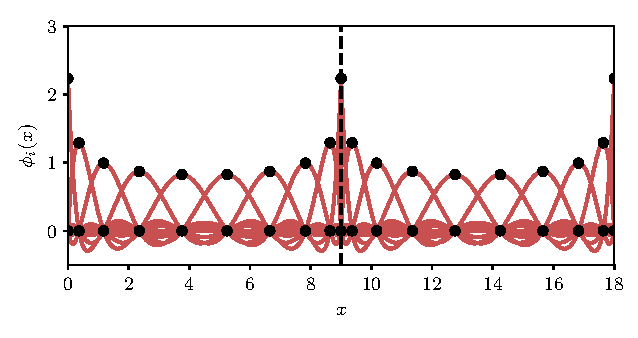
\includegraphics{figures/numerics/fedvr_basis.pdf}
    \caption{An example of the normalised, but non-orthogonal basis polynomials used in the finite-element discrete variable representation, shown here for ten-point Gauss--Lobatto quadrature and two elements. Note that each basis polynomial is nonzero at exactly one point and zero at all others, though it can be nonzero in between points. Outside of its element, a given basis function is defined to be zero, except for the so-called ``bridge functions", which are nonzero in two adjacent elements but zero everywhere else, and surprisingly have a discontinuous derivative at the boundary---necessitating some care in evaluating matrix elements of differential operators.}
    \label{fig:fedvr_basis}
\end{figure}

By choosing a quadrature scheme with two points located exactly on each edge of the integration regions, such as \emph{Gauss--Lobatto} quadrature \cite{schneider_discrete_2005}, the elements of the \textsc{fedvr} method can be joined together, with adjacent elements sharing these edge points (see \figref{fig:fedvr_basis}). This allows one to represent a wavefunction as a list of coefficients for how much of each basis polynomial in each element contributes to it, with the extra condition that some of these coefficients---those corresponding to the edge points---must be equal in order to ensure the wavefunction is continuous across the boundaries between elements.

With some care taken in regard to the points shared between the elements, the \textsc{fedvr} method provides one with a means of approximating wavefunctions as a finite sum of basis functions, and of approximately calculating the matrix elements of operators in this basis. After that, one can simply apply the operators to the state vectors in order to compute time derivatives, and propagate in time using fourth order Runge--Kutta (section \ref{sec:rk4}) or similar, or one can exponentiate the operators, all at once or one at a time, as part of a split-step method (section \ref{sec:split-step}). The \textsc{fedvr} method does not require anything in particular about time propagation---like finite differences or the Fourier pseudospectral method, it is only a way of spatially discretising the differential equation you are trying to solve.

Now we arrive at what makes the \textsc{fedvr} method exciting for those who want to massively parallelise their simulations. When one calculates the matrix representation of, say, a one-dimensional differential operator in the \textsc{fedvr} basis, one gets matrices that look like \figref{fig:fedvr_D2_operator}, with an almost-block-diagonal form.

\begin{figure}[t]
    \centerfloat
    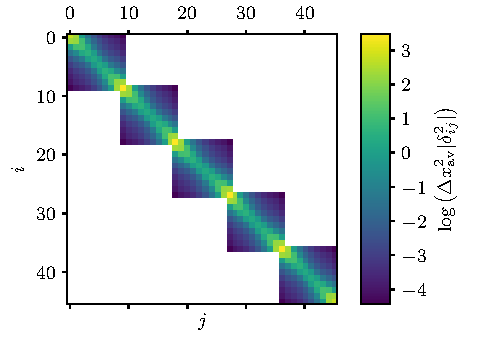
\includegraphics{figures/numerics/fedvr_D2_operator.pdf}
    \caption{The matrix form of the second derivative operator in \textsc{fedvr}, for five elements each with ten \textsc{dvr} points. The colour scale is logarithmic, showing the log of the absolute values of the matrix elements $\delta^2_{ij}$ scaled by $\upDelta x_\up{av}^2$, where $\upDelta x_\up{av}$ is the average spacing between the unequally spaced grid points. Zero matrix elements are shown as white. One can see that the second derivative at each grid point is computed using only the points within the same element, except for the points shared by adjacent elements, at which the second derivative depends on points in both adjacent elements.}
    \label{fig:fedvr_D2_operator}
\end{figure}

 This is because when the state vector is acted upon by some operator, the result for most points in the resulting vector depends only on the points in the input vector \emph{within the same element}. The exceptions are the points shared between elements---for which the value in the output vector depends on the points in the input vector in \emph{both} adjacent elements, which is why the matrix is not perfectly block diagonal.

Why is this exciting? Well, it means that the operator can be written as a sum of two block diagonal matrices, similar to the splitting of finite-difference matrices in section \ref{sec:split-step-parallel}, and in the same way allows the matrix or its exponentiation to be efficiently applied to a state vector in parallel. The difference between this and the case of finite differences is the number of points of overlap between adjacent blocks, which corresponds to the amount of data that must be transferred between parallel threads or cluster nodes at each step during a parallel computation. In finite differences, the number of points that must be exchanged at boundaries in each step or sub-step of whichever time propagation method is used is equal to the bandwidth of the matrix. In \textsc{fedvr}, so long as the boundaries of the regions of space assigned to each thread or cluster node align with boundaries between elements, \emph{only one} point need be exchanged. Increasing the number of points within each element---but reducing the number of elements so as to keep the total number of points constant, decreases the discretisation error of the method, but still, only one point needs to be exchanged at boundaries. This contrasts with finite differences, for which increasing the order of the finite difference scheme increases the matrix bandwidth and hence increases the number points required to be exchanged at the boundaries. So it would seem that \textsc{fedvr} ought to scale much better in parallel implementations, which is a large part of its appeal \cite{schneider_discrete_2005,schneider_parallel_2006}.

However, I've noticed that when using both \textsc{fedvr} and finite differences to simulate Bose--Einstein condensates using the Gross--Pitaevskii equation, smaller timesteps are required when using the \textsc{fedvr} method in otherwise comparable setups. By this I mean that, without damping, there is a timestep size at which the \textsc{gpe} simulated using \textsc{rk4} (which is a conditionally stable algorithm) is unstable and diverges. Similarly in split-step methods, although the error is bounded, there is a timestep size at which the error rapidly grows to that bound and the wavefunction no longer approximately resembles the true solution. Below this threshold timestep, the error scales as $\Ord{\upDelta t^4}$ for \textsc{rk4}, and $\Ord{\upDelta t^4}$, $\Ord{\upDelta t^2}$, $\Ord{\upDelta t}$ for fourth, second, and first order split-step respectively, as expected. But in practice, all these methods are so accurate that one desires to use the largest timestep one can without this blowup (or soft-blowup in the case of the unitary split-step methods) occurring during the time interval one wants to simulate. And my observation was that the threshold timestep is always smaller for \textsc{fedvr} than for finite differences or the Fourier method for determining spatial derivatives, necessitating smaller timesteps for stability or, in the case of the unitary methods, reasonable accuracy.

So why is this? For \textsc{rk4}, what is the stability criterion and why might \textsc{fedvr} violate it more easily than finite differences? And how might we understand the sudden decrease in accuracy of the split-step methods at a similar threshold timestep size, despite them being unconditionally stable?

The stability critereon for \textsc{rk4} when applied to a linear differential equation of the form:

\begin{align}
\dv{\vec\psi}{t} = A\vec\psi,
\end{align}
where A is a matrix with all imaginary eigenvalues (as is the case for Hamiltonian evolution where $A=-\frac \ii \hbar H$), is\cite{caplan_numerical_2011}:
\begin{align}
\upDelta t < \frac{2 \sqrt 2}{\rho(A)}
\end{align}
where $\rho(A)$ is the \emph{spectral radius} of $A$, defined as the absolute value of the largest (by absolute value) eigenvalue of $A$.

The Gross--Pitaevskii equation is not linear, but we'll put that to the side for the moment---it will be relevant shortly. In the linear case of the Schr\"odinger wave equation, an upper bound for the spectral radius of $A$ can be computed from the absolute eigenvalue from the kinetic term, plus the maximum absolute eigenvalue from the potential term. Using the Fourier method to compute spatial derivatives, the largest eigenvalue of the kinetic part of the Hamiltonian is that of the Nyquist mode with $k_\up{Nyquist} = \pi / \upDelta x$ for grid spacing $\upDelta x$, leading to:
\begin{align}
\rho(A) &\leq \Abs{-\frac \ii \hbar \frac{\hbar^2 k_\up{Nyquist}}{2m}}
+ \Abs{-\frac \ii \hbar V(\vec r)}_\up{max}\\
\Rightarrow \upDelta t &< \frac{2\sqrt 2 \hbar}
{\frac{\hbar^2\pi^2}{2m \upDelta x^2} + \abs{V(\vec r)}_\up{max}}.
\end{align}
In the limit of small $\upDelta x$, the kinetic term dominates and the stability criterion becomes:
\begin{align}\label{eq:rk4_kinetic_stability}
\upDelta t &< \frac{4\sqrt 2 m \upDelta x^2}{\pi^2 \hbar},
\end{align}
whereas in the limit of large potential:
\begin{align}
\upDelta t &< \frac{2\sqrt 2\hbar}{\abs{V(\vec r)}_\up{max}}.
\end{align}
These results match our intuition somewhat in terms of dynamical phase evolution---eigenvalues of the Hamiltonian are energies and determine how quickly the elements of the state vector accumulate dynamical phase. For each circle around the complex plane that a dynamical phase of $2\pi$ entails, we expect to require at least a few timesteps to resolve said circle, and the above shows that `a few' means $2\sqrt{2}$. When this dynamical phase evolution is in Fourier space, an accumulated phase of $2\pi$ will appear in real space as that component having propagated a distance of one wavelength, so the intuition here is that several timepoints are required in the time interval during which the fastest wave (also the Nyquist mode) propagates a distance of one wavelength at its phase velocity.

As a sidenote, if it is known which term of the Hamiltonian dominates the stability criterion, that term can be removed by use of an \emph{interaction picture} (discussed in section \ref{sec:rk4ilip}), essentially treating the dynamical phase evolution due to that term analytically. And if the term is not constant, but is \emph{almost} constant, one can still treat \emph{most} of the dynamical phase evolution analytically, transforming the differential equation onto one with much smaller eigenvalues for that term, in both cases allowing one to take potentially much larger timesteps due to the above reasoning. Fourth order Runge--Kutta in the interaction picture (\textsc{rk4ip}) \cite{caradoc_davies_thesis} uses an interaction picture to treat the kinetic term of the Schr\"odinger or Gross--Pitaevskii equation analytically, whereas my `fourth order Runge--Kutta in an instantaneous, local interaction picture' method presented in section \ref{sec:rk4ilip} removes (most of) the potential term. Both methods allow larger timesteps to be taken, but in different circumstances depending on which term is dominating the Hamiltonian.

The problem with \textsc{fedvr} then, is that it requires smaller timesteps than finite differences because its kinetic energy operator has larger eigenvalues than an equally accurate finite difference method. How much larger?

In order to make a fair comparison, we need to know how many \textsc{dvr} basis functions are required per element in order to compute equally accurate second derivatives as a given finite difference scheme. With $N$ points per element, \textsc{fedvr} represents the state vector within each element in a spectral basis of polynomials up to degree $N - 1$. Therefore a polynomial of degree $N - 1$ or less can be represented exactly, any other function is subject to truncation error\footnote{Note that this truncation error is distinct from that of evaluating \emph{integrals} using the Gauss--Lobatto quadrature rule, which is exact for integrands that are polynomials of degree $2N - 2$ or less.}. If one varies the number of points per element, varying the number of elements in order to keep the total number of points constant, the truncation error in representing an arbitrary function in this basis is therefore $\Ord{\upDelta x^N}$, where $\upDelta x$ is either the size of each element, or equivalently the average spacing between grid points (these two differing only by a constant factor if the total number of points is held constant).

In \textsc{fedvr} the derivative operator, regardless of whether its matrix elements are computed with integrals or the quadrature rule, is exact \cite{schneider_discrete_2005}. The relevant error in a derivative of a wavefunction is therefore determined by this truncation error of representing it in the spectral basis in the first place:

\begin{align}
\psi_\up{approx}(x_i) = \psi_\up{exact}(x_i) + \Ord{\upDelta x^N}\\
\Rightarrow\psi^{\prime \prime}_\up{approx}(x_i) =  \psi^{\prime\prime}_\up{exact}(x_i) + \Ord{\upDelta x^{N-2}}.
\end{align} 

Central finite difference approximations to second derivatives on the other hand have error $\Ord{\upDelta x^{N - 1}}$ where N is the total number of points used to compute the derivative at each point (for example the three-point central finite difference rule for second derivatives has error $\Ord{\upDelta x^2}$, the five-point rule is accurate to $\Ord{\upDelta x^4}$, etc). With this knowledge we can translate our question

\begin{quote}
Which is less computationally intensive to simulate the \textsc{gpe} or Schr\"odinger wave equation: $m^\up{th}$-order accurate \textsc{fedvr} or $m^\up{th}$-order accurate finite differences?
\end{quote}
to
\begin{quote}
which is less computationally intensive to simulate the \textsc{gpe} or Schr\"odinger wave equation: $m+2$ points-per-element \textsc{fedvr} or $m+1$ point central finite differences?
\end{quote}
The argument in favour of \textsc{fedvr} is that as $m$ grows, finite differences require an increasing number of points to be exchanged at the boundaries between cluster nodes/threads etc in a parallel implementation, whereas so long as each boundary between spatial regions allocated to different cluster nodes aligns with the boundary between two elements, only one point need be exchanged per timestep in \textsc{fedvr}, no matter how many points per element there are. Therefore, in the limit of high accuracy, \textsc{fedvr} wins, it seems.

The problem with this argument is that it compares only the amount of work that needs to be done \emph{per timestep}. But, since the allowed timestep size required for stability (at least for fourth order Runge--Kutta, I'll argue shortly why I think this generalises to other timestepping schemes as well) depends on the spectral radius of the kinetic energy operator, and the kinetic energy operator is not the same as $m$ grows, more work is needed to show which method is least computationally expensive per unit \emph{simulation time}.

The spectral radius of the kinetic energy operator when approximated using central finite differences does not grow without limit as the number of points used to compute derivatives increases---indeed, its eigenspectrum converges to that of the Fourier method (since the Fourier method can be considered the limit of `infinite order' finite differences \cite{fornberg_pseudospectral_1987}), with maximum eigenvalue equal to the kinetic energy of the Nyquist mode. The kinetic energy operator approximated with \textsc{fedvr} on the other hand does not have a bounded spectral radius as one increases the number of points per element whilst holding the total number of gridpoints constant. Instead its spectral radius increases quadratically with the number of points (equivalently with the order of accuracy of the derivatives), as shown in \figref{fig:fedvr_eigenvalue_scaling}.

\begin{figure}[t]
    \centerfloat
    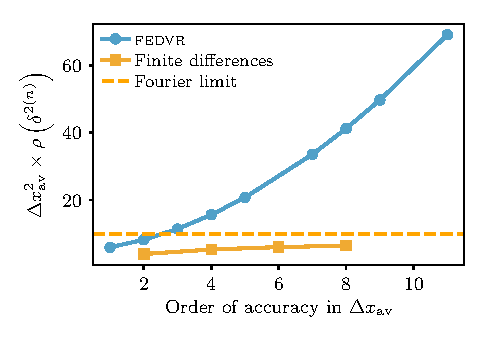
\includegraphics{figures/numerics/fedvr_eigenvalue_scaling.pdf}
    \caption{Scaling of the spectral radius (maximum absolute eigenvalue) of the second derivative operator with respect to the order of accuracy for finite differences and \textsc{fedvr}. Results were numerically computed by constructing a $721\times721$ matrix (chosen to allow various combinations of number of \textsc{dvr} points per element whilst holding total number of points constant) for each order of accuracy and numerically diagonalising. The spectral radius for \textsc{fedvr} can be seen to scale quadratically with the order of accuracy, whereas for finite differences the maximum eigenvalue approaches that of the Fourier method.}
    \label{fig:fedvr_eigenvalue_scaling}
\end{figure}

This result ought to be expected, at least qualitatively. The density of points in \textsc{fedvr} is higher toward the edges of the elements than in their centres, and if one increases the number of points per element whilst decreasing the number of elements so as to hold the total number of points approximately constant, the smallest spacing between any two adjacent points will be inversely proportional to the number of points per element. We already know that in high order finite differences or the Fourier method, the spectral radius of the kinetic energy operator is simply the kinetic energy of the Nyquist mode, and being the mode described by a wave with half a wavelength spanning one grid spacing, its kinetic energy is proportional to the square of the grid spacing. It not therefore surprising that in \textsc{fedvr} when the grid spacing is linearly smaller---albeit locally---that the spectral radius of the kinetic energy operator is quadratically larger. The same result as above could be obtained by asking: ``what is the smallest grid spacing, and what is the kinetic energy of the Nyquist mode corresponding to that grid spacing"?, and then declaring the stability criterion to be that one must have at least a few points per period of the frequency corresponding to that energy.

Since the spectral radius of \textsc{fedvr} operators grows faster with increasing order of accuracy in derivative operators than finite differences, \textsc{fedvr} requires smaller timesteps for stability when used with \textsc{rk4}. Even at low order accuracy, finite difference operators have smaller spectral radii, and so at all levels of accuracy \textsc{rk4} is stable with finite differences for larger timesteps than with \textsc{fedvr}. In the limit of high accuracy then, compared to finite differences \textsc{fedvr} requires \emph{quadratically} more timesteps to be taken for stability, whereas it requires only \emph{linearly} fewer points to be transferred at the boundaries between threads or cluster nodes per timestep. The larger number of timesteps is therefore the dominant effect, more than cancelling out the benefit of having to transfer fewer points at boundaries per timestep than with finite differences. Indeed, even if transferring data between nodes or threads is the bottleneck of a parallel simulation, \emph{more} points are being transferred all up with \textsc{fedvr}---they are just spread out over more timesteps.

That's fourth order Runge--Kutta. What about split-step methods? The split-step methods discussed in section \ref{sec:split-step} are unconditionally stable and have bounded error. However, their error can still be large enough to make the results not useful. As shown in \eqref{eq:commutation_error}, the leading error term in first-order split-step is $1/2\hbar^2[V, K]\upDelta t^2$ where $[V, K]$ is the commutator between the (discretised) kinetic and potential energy operators. The leading term of $V$ is proportional to the discretised $\hat x$ operator $X$, and the kinetic energy operator is proportional to an $n^\up{th}$ order accurate discretised second derivative operator $\delta^{2 (n)}$. Therefore the error per timestep scales with $[X, \delta^{2 (n)}]\upDelta t^2$. Although this expression is not bounded, the error in first-order split-step is nonetheless bounded because this error appears as the argument of a complex exponential. When expanding the complex exponential as its Taylor series, this error term is the leading term, but when it grows it leads merely to a complex exponential with unbounded phase error, not to unbounded absolute error. Nonetheless unbounded phase error still makes the results of a simulation unlikely to be useful.

The largest (by absolute value) eigenvalue of this commutator sets the rate at which erroneous dynamical phase is accumulated by some eigenstate of the commutator. When this phase becomes comparable to $2\pi$ per timestep, the simulation has clearly lost any semblance of accuracy, despite still being technically ``stable". Therefore as before, the spectral radius of the matrix of this commutator can be used to define a \emph{pseudo}-stability criterion, such that when the spectral radius of $[V, K]\upDelta t^2/2\hbar^2$ becomes comparable to unity, the error will dominate the simulation results. Although the value of the spectral radius will depend on the details of the potential energy operator $V$ for the particular problem, we can still ask how it scales with increasing order of accuracy of $K$ given that $X$ is the leading term of $V$. This is done in \figref{fig:fedvr_commutation_error_scaling}, comparing the spectral radius of the commutator when using derivative operators of various orders in both finite differences and \textsc{fedvr} approximations.

\begin{figure}[t]
    \centerfloat
    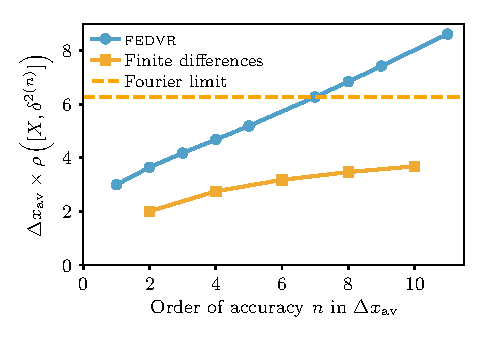
\includegraphics{figures/numerics/fedvr_commutation_error_scaling.pdf}
    \caption{Scaling with order of accuracy of the spectral radius of the commutator of position and second derivative operators in the pseudospectral finite difference method and \textsc{fedvr}. The spectral radius of the commutator grows linearly with increasing order of accuracy for \textsc{fedvr}, whereas it is bounded for finite differences, approaching that of the Fourier method.}
    \label{fig:fedvr_commutation_error_scaling}
\end{figure}

The result is that as with \textsc{rk4}, the pseudo-stability criterion allows at all orders of accuracy for larger timesteps when using finite differences than when using \textsc{fedvr}, and that the required timestep is bounded from below when increasing the order of accuracy of finite differences, but can become arbitrarily small for increasing accuracy of \textsc{fedvr}. However the situation is not so dire for \textsc{fedvr} when used with split-step as it is with \textsc{rk4} timestepping. Because the error term in split-step is this commutator multiplied by $\upDelta t^2$, the timestep required for pseudo-stability scales inversely with the \emph{square root} of the spectral radius of the commutator---not with the spectral radius itself as with \textsc{rk4}. Furthermore the spectral radius of the \textsc{fedvr} commutator increases only \emph{linearly} with increasing order of accuracy, not quadratically as with \textsc{rk4}. Therefore if transferring data between nodes (with time cost proportional to the amount of data transferred) is the bottleneck of one's simulation, then with increasing accuracy, \textsc{fedvr} \emph{does} win out. For high enough order of accuracy $n$, a factor of $\sqrt{n}$ more timesteps are needed with \textsc{fedvr} compared to finite differences, but a factor of $n$ \emph{fewer} points are sent per timestep. This results in a factor of $1/\sqrt{n}$ fewer points being sent per unit simulation time with \textsc{fedvr} as compared to finite differences. The question of which method is faster then comes down to which is more costly: extra timesteps, or extra data transfer? Using \textsc{fedvr} will save you a factor of $\sqrt{n}$ in data transfer at a cost of a factor of $\sqrt{n}$ in the number of timesteps. Given InfiniBand interconnects on cluster computers with tens of gigabits per second of bandwidth, and latency that does not scale with the amount of data, I suspect that a $\sqrt{n}$ increase in cost of processing within nodes/threads is almost always the larger cost to pay. Therefore I suspect the benefits of \textsc{fevdr} for parallel simulations of the Schr\"odinger wave equation or Gross--Pitaevskii equation are limited.

\subsection{Nonlinearity considerations}

The above arguments about stability all disregarded the nonlinearity of the Gross--Pitaevskii equation. Although the stability of a numerical method is very difficult to analyse for nonlinear differential equations, there is a simple argument for heuristically putting an upper bound on the timestep required in order to accurately model the effect of the \textsc{gpe}'s nonlinear term. Essentially, density waves in the condensate propagate not at the phase velocity of the condensate wavefunction, but at its group velocity. The group velocity of the shortest possible wavelength in the system therefore sets an upper bound for the propagation of information due to the nonlinear term. In order to correctly model this term, timesteps must be short enough that one's numerical method is evaluating the nonlinear term frequently enough that fast moving density waves can't `skip` gridpoints in between evaluations. If the smallest wavelength is that of the Nyquist mode, or for nonuniform grids the mode whose wavelength is twice the smallest grid spacing, then the maximum group velocity is:

\begin{equation}
v_\up{g}(k_\up{max}) = \pdv{E_\up{K}(k_\up{max})}{p(k_\up{max})} =  \frac{\hbar k_\up{max}}{m}\frac{\pi \hbar}{m \upDelta x_\up{min}}
\end{equation}

Asking how long it takes a wave to move a distance of $\upDelta x_\up{min}$ at this velocity then results in what I'm calling the \emph{dispersion timescale}:

\begin{equation}
\tau_\up d = \frac{m\upDelta x_\up{min}^2 }{\pi \hbar}.
\end{equation} 

The numerical method being used is now fairly irrelevant: one must evaluate the nonlinear term at least as often as every $\tau_\up d$ in order to be able to model it accurately, otherwise density waves may move past each other faster than they can be resolved by the timestepping, and their interference patterns will be aliased by the too-slow timestepping, resulting in incorrect nonlinear dynamics.

Note that up to constant factors, this criterion for accurate modelling is the same as the stability criterion \eqref{eq:rk4_kinetic_stability} for \textsc{rk4} when the kinetic term dominates the Hamiltonian. Therefore although first-order split-step as argued above appears to be more forgiving to \textsc{fedvr} than \textsc{rk4} is, this is no longer the case when modelling the \textsc{gpe} as opposed to the linear Schr\"odinger wave equation, and although I didn't extend the argument in the previous section to second or fourth order split-step (figuring out which commutator is the leading term is much more involved), they too are subject to the same requirement to sample the nonlinear term this frequently, even if their linear pseudo-stability region might be larger.

\subsection{Conclusion}

\begin{figure}[t]
    \centerfloat
    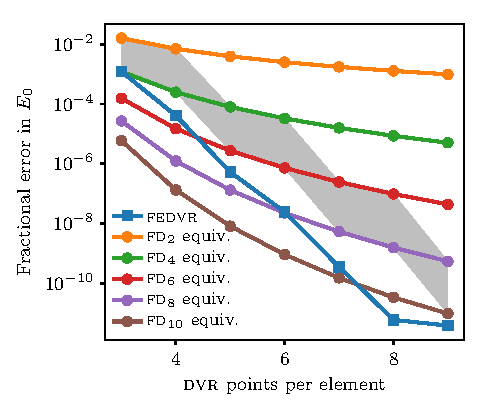
\includegraphics{figures/numerics/fedvr_vs_fd_harmonic_groundstate.pdf}
    \caption{TODO CAPTION once mentioned in text}
    \label{fig:fedvr_vs_fd_harmonic_groundstate}
\end{figure}

\begin{figure}[t]
    \centerfloat
    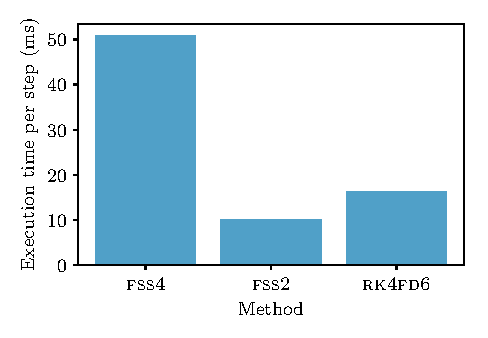
\includegraphics{figures/numerics/method_speeds.pdf}
    \caption{TODO CAPTION once mentioned in text, not sure where to mention this in-text.}
    \label{fig:method_speeds}
\end{figure}

\begin{figure}[t]
    \centerfloat
    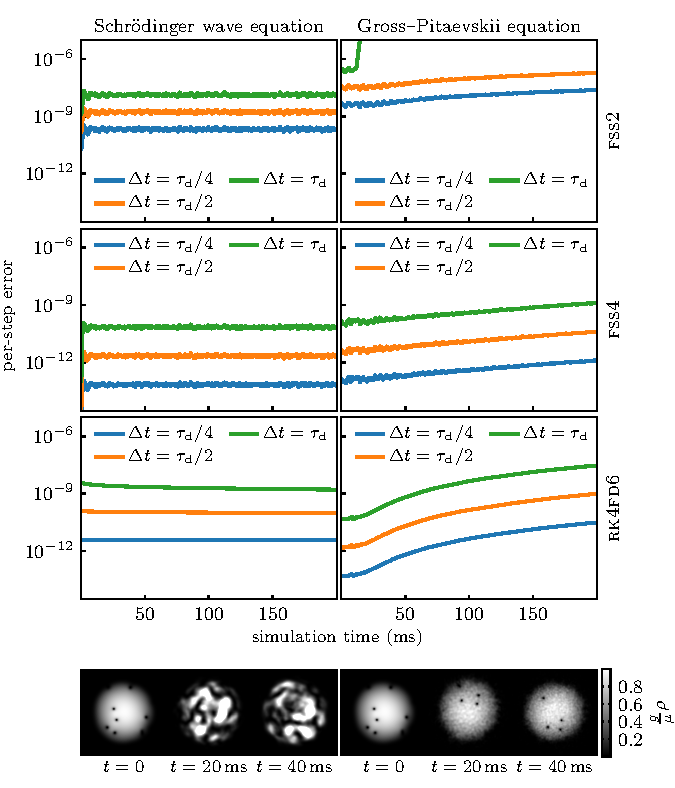
\includegraphics{figures/numerics/stability.pdf}
    \caption{TODO CAPTION once mentioned in text, not sure where to mention this in-text.}
    \label{fig:stability}
\end{figure}

This leaves us with little remaining benefit to \textsc{fedvr} over finite differences for the Schr\"odinger wave and Gross--Pitaevskii equations. The argument that \textsc{fedvr} scales better for parallel computation is unconvincing as argued above. The fact that it allows nonuniform grids is also not unique---central finite differences allow for nonuniform grids as well \cite{fornberg_generation_1988}. Reference \cite{schneider_parallel_2006} compares the accuracy of finite differences to \textsc{fedvr} in the context of computing the groundstate energy of a harmonic oscillator using imaginary time evolution (see section \ref{sec:ITEM}), but only uses second-order finite differences in the comparison whereas higher-order \textsc{fedvr} schemes are used. If this restriction was in order to hold the number of points transferred at boundaries between parallel computing units constant (since second-order finite differences require, like \textsc{fedvr}, only one per timestep), then this is not an equal comparison as the number of points transferred does not limit computation time as I've shown---had the authors included comparisons with higher order finite differencing schemes, they would have resulted in comparable accuracy (see \figref{fig:fedvr_vs_fd_harmonic_groundstate}) between \textsc{fedvr} and finite differences, but with finite differences completing in in less time owing to the larger timesteps allowed by the increased range of stability of finite differences.

Perhaps for problems with certain unusual boundary conditions or strangely shaped regions, or where one can construct a geometric integrator that conserves some quantities of interest other than merely the wavefunction norm, \textsc{fedvr} may still make sense. But unless there is a compelling reason, it seems that simple finite differences, as naïve as it might seem at first, remains a practical choice for highly accurate and potentially massively parallelised simulations of the \textsc{gpe}.

\section{Finding ground states}

For systems with continuous degrees of freedom, such as Bose--Einstein condensates, finding groundstates by directly diagonalising the Hamiltonian matrix is impractical due to the size of said matrix, which we normally avoid even constructing for systems with more than one dimension when simply propagating condensate wavefunctions in time. The pseudo-Hamiltonian for the Gross-Pitaevksii equation is not even linear, implying direct diagonalisation would not even return groundstates unless one diagonalised matrices repeatedly, each with an improved estimate of the groundstate until a self-consistent solution was found.

Below are two methods that are typically used instead to find groundstates in these cases, as well as a generalisation (which only applies to linear systems) for finding other excited states of quantum systems.

\subsection{Imaginary time evolution}\label{sec:ITEM}

Imaginary time evolution [CITE] is a robust, if somewhat inefficient method of finding groundstates of quantum systems, and can be generalised to finding excited states as well (Section \ref{sec:excited_states_gram_schmidt}, below). The basis idea is to evolve the following differential equation:
\begin{align}\label{eq:ITEM}
\hbar\dv{\vec\psi}{t} = - H \vec \psi
\end{align}
in time instead of the time-dependent Schr\"odinger equation \eqref{eq:schrodinger_equation_matrix_vector}, for some wavefunction or state vector $\vec \psi$ and matrix/linear operator $H$. The name \emph{imaginary time evolution} is due to the fact that this differential equation can be obtained by making the substitution $t\rightarrow - \ii t$ in the time-dependent Schr\"odinger equation, and hence can be thought of as propagating the Schro\"odinger equation in (negative) imaginary time. This method is capable of evolving an initial guess for $\vec \psi$
into the groundstate of the given Hamiltonian. The reason behind this can be seen if we rewrite \eqref{eq:ITEM} in the eigenbasis of $H$ with eigenvalues $\{E_n\}$ and eigenkets $\{\ket{n}\}$:
\begin{align}
\hbar \dv t \braket{n}{\psi(t)} = - E_n \braket{\phi_n}{\psi(t)},
\end{align}
which has solutions:
\begin{align}
\braket{n}{\psi(t)} = \exp\left[- \frac{E_n}\hbar t\right]\braket{n}{\psi(0)},
\end{align}
that is, the coefficient of each eigenstate exponentially decays with a decay rate proportional its energy. After enough time has elapsed (much larger than the difference in decay timescales between the two lowest lying eigenstates), all coefficients $\braket{n}{\psi(t)}$ will have decayed, but the coefficient corresponding to the groundstate will have decayed by far the least, leading to any initial superposition evolving into one dominated by the groundstate.

This method is flexible and robust, and can be used to find groundstates subject to imposed conditions such as a phase winding about a point, resulting in a vortex state. It can also be used to `smooth' candidate wavefunctions, making a guessed initial state of a condensate wavefunction more like a physically realistic one by lowering its energy somewhat, but not propagating far enough to obtain the actual groundstate. This smoothing method is used in Section \ref{sec:rk4ilip} to create an approximately correct density profile for a condensate wavefunction after the phase patterns for randomly distributed vortices are artificially imposed, resulting in physically realistic initial conditions for a turbulent condensate.  

For practical reasons, exponential decay cannot be carried out indefinitely, as eventually all numbers underflow to zero as they become too small to be represented on a computer. In addition, the wavefunction/state vector obtained after exponential decay will not be normalised. For these reasons, one often normalises the wavefunction/state vector to unit norm in between each step of imaginary time evolution.

Normalisation must be paid attention particularly in the case of the Gross--Pitaevskii equation, since it has a nonlinear pseudo-Hamiltonian. This pseudo-Hamiltonian must always be evaluated with a normalised condensate wavefunction as input, otherwise the imaginary time evolution may, depending on the numerical method employed, produce a final condensate wavefunction which is the groundstate not in the presence of the actual nonlinear term, but in the presence of one that has had one timestep worth of exponential decay applied to it. Since the magnitude of the wavefunction matters in the Gross--Pitaevskii equation, one must normalise every time a nonlinear $H$ is evaluated in order to prevent this problem (which can also be mitigated by taking tiny timesteps to minimise the amount of decay within each timestep, but this is wasteful when larger steps could otherwise be used).

An exception to the above normalisation warning is when a first order explicit method such as the first-order split step method [SECREF] or the Euler method is used---since these methods only ever evaluate the nonlinear pseudo-Hamiltonian at the start of a timestep, normalising the wavefunction once per timestep is sufficient, whereas when using higher order methods that evaluate the pseudo-Hamiltonian at intermediate times one will have to take care to normalise more often.

The imaginary time evolution method is a \emph{relaxation method}, and as such only the final wavefunction/state vector after a sufficient period of evolution is of interest, not the intermediate states. As such, inaccurate but fast methods such as first order split-step or the Euler method may be readily employed, and used with the largest timesteps that do not lead to numerical instability. Second order Runge--Kutta (the explicit midpoint method) can be a good balance due to being faster per-step than more accurate methods, whilst allowing larger timesteps than the Euler method due to better stability characteristics.

A final note is that energies of quantum systems are arbitrary up to a global additive constant, and so energies can be negative or positive or some mix of both in the same system. In this case, imaginary time evolution can have some or all coefficients of energy eigenstates exponentially \emph{growing} rather than decaying. This does not modify the end result at all, as the groundstate energy, if negative, will be more negative than any other energy and hence its coefficient will exponentially grow faster than all others. If an estimate of the groundstate energy is known ahead of time, it can be advantageous to offset the system Hamiltonian with a constant energy such that the groundstate energy is approximately zero, which minimises the amount of exponential growth/decay and allows for the largest timesteps within the stability range of the numerical method employed. One can even dynamically compute an energy or chemical potential estimate\footnote{Note that the energy of a BEC using the Gross--Pitaevsii pseudo-Hamiltonian cannot be computed simply as the expectation value of the pseudo-Hamiltonian---this double counts the nonlinear term, which should be halved in such energy calculations. The chemical potential however can be computed as this expectation value.} to update the energy offset as the computation proceeds. Imaginary time evolution can be slow enough for non-trivial cases that these considerations can be relevant.

Since imaginary time evolution comprises the evolution of a state vector in time, it is amenable to all the parallel processing techniques we have outlined in this chapter depending on the timestepping and spatial discretisation employed.

\subsection{Successive over-relaxation}\label{sec:SOR}

Successive over-relaxation (\textsc{sor}) [CITE] is a much faster method of finding groundstates than imaginary time evolution, but slightly less flexible. Strictly speaking, \textsc{sor} can solve linear systems of the form:
\begin{align}\label{eq:linear_system_SOR}
A \vec \psi = \vec b,
\end{align} 
for some unknown vector (or discretised function) $\vec \psi$ given a vector (or discretised function) $\vec b$ for the right hand side and a  matrix (or discretised linear operator) $A$ for the left hand side. The method is of most benefit when $A$ is diagonally dominant, lending \textsc{sor} to use with finite difference methods. As with imaginary time evolution, \textsc{sor} requires an initial guess for $\vec\psi$ that is repeatedly updated to produce an increasingly accurate approximate solution to the given linear system.

Successive over-relaxation proceeds by updating each element $\psi_i$ of $\vec\psi$ one at a time to be more consistent with the linear system and all other estimated elements of $\vec\psi$. To update each element of $\vec\psi$, we first write a single element of the vector equation \eqref{eq:linear_system_SOR} as
\begin{align}
\sum_j A_{ij}\psi_j = b_i
\end{align}
and separate out the $i^\up{th}$ term of the matrix multiplication sum:
\begin{align}
A_{ii}\psi_i + \sum_{j\neq i} A_{ij}\psi_j = b_i,
\end{align}
and solve for $\psi_i$:
\begin{align}
\psi_i = \frac{b_i - \sum_{j\neq i} A_{ij}\psi_j}{A_{ii}},
\end{align}
which is the value a single element $\psi_i$ should be updated to in order to become consistent with all other elements $\psi_{j\neq i}$ and the linear system. If one updates every element of $\vec\psi$ in this manner, based on values of $\vec\psi$ at the previous iteration, the method that results is called the Jacobi method [CITE]:
\begin{align}
\psi^{(k+1)}_{i\,\up{Jacobi}} = \frac{b_i - \sum_{j\neq i} A_{ij}\psi^{(k)}_j}{A_{ii}},
\end{align}
where $\vec\psi^{(k)}$ is the $k^\up{th}$ iterative estimate of $\vec\psi$.
If one allows use of already updated elements of $\vec\psi$ when updating subsequent elements of $\vec\psi$, one obtains the more efficient Gauss--Seidel method [CITE]:
\begin{align}\label{eq:GaussSeidel}
\psi^{(k+1)}_{i\,\up{GS}} = \frac{b_i - \sum_{j\neq i} A_{ij}\psi^{(\up{latest})}_j}{A_{ii}},
\end{align}
where $\psi^{(\up{latest})}_j = \psi^{(k+1)}_j$ if $\psi^{(k+1)}_j$ has been computed already, and $\psi^{(k)}_j$ if not. Assuming elements of $\vec\psi$ are updated in order of increasing $j$, one can split the sum into two for these two cases and write:
\begin{align}
\psi^{(k+1)}_{i\,\up{GS}} = \frac{b_i - \sum_{j<i} A_{ij}\psi^{(k+1)}_j - \sum_{j>i} A_{ij}\psi^{(k)}_j}{A_{ii}},
\end{align}
which is how the method is often presented; however, since one can update elements in any order (or equivalently, the order of the basis vectors in $\vec\psi$ is arbitrary), I prefer the form \eqref{eq:GaussSeidel} as it leaves the iteration order undetermined. One reason to impose an update order other than just that of increasing index in the array storing $\vec\psi$ in computer memory is to minimise communication latency in parallel implementations: one may choose to update points near one or more edges of the spatial region assigned to one \textsc{cpu} core or cluster node first, in order that they become available to other cores/nodes sooner, before updating the interior points that other cores/nodes do not depend on. In this case of parallel processing there isn't even a strict order since elements are being updated independently by separate cores/nodes simultaneously. Gauss--Seidel and successive over-relaxation still work well in this case, they just become a little more like the Jacobi method the more independent updates are occurring on different parts of the vector $\vec\psi$.

The final feature of successive over-relaxation is that elements of $\vec\psi$ are updated not to the values given by the Gauss--Seidel method, but overshoot them by a factor $\alpha$:
\begin{align}\label{eq:SOR}
\psi^{(k+1)}_{i\,\textsc{sor}} = \psi^{(k)}_i + \alpha\left(\frac{b_i - \sum_{j\neq i} A_{ij}\psi^{(\up{latest})}_j}{A_{ii}} - \psi^{(k)}_i\right).
\end{align}
where $\alpha < 2$ is the convergence criterion [CITE] in the case of an infinite system.\footnote{With the deviation from strict \textsc{sor} by using non-constant $A$ and $\vec b$ mentioned below, and parallel updates as mentioned above, as well as the fact that systems are not infinite, $\alpha$ in the range of $1.6$ to $1.8$ is realistic to ensure stability in Gross--Pitaevskii equation simulations.}

So what are $A$ and $\vec b$ for quantum mechanics problems? One deviation from pure \textsc{sor} used in cold atom physics is to allow both $A$ and $\vec b$ to have dependence on $\vec\psi$, which in practice does not prevent the method from finding solutions. For the groundstate of the Gross--Pitaevskii equation, we can write:
\begin{align}\label{eq:GPE_SOR}
H(\vec\psi)\vec \psi &= \mu\vec \psi
\end{align}
where $\mu$ is the chemical potential of the condensate in its groundstate and $H(\vec\psi)$ is the matrix for some discretisation of the Gross--Pitaevskii pseudo-Hamiltonian\footnote{A subtle consequence of $A$ and $\vec b$ depending on $\vec\psi$ is that we cannot simplify this to $(H(\vec\psi) - \mu)\vec \psi = \vec0$, as this would admit $\vec\psi=\vec0$ as a solution. As written, \eqref{eq:GPE_SOR} also admits $\vec\psi=\vec0$ as a solution, however, $A^{(k)} = H(\vec\psi^{(k)})$ and $\vec b^{(k)} = \mu\vec\psi^{(k)}$ are treated as constants within a single iteration of \text{sor}, preventing the method from approaching zero as a solution compared to if $\psi$ was present only on the left hand side.}, to which we can then apply a single iteration of \textsc{sor} by updating all elements of $\vec\psi$ in some order using \eqref{eq:SOR} with $A^{(k)} = H(\vec\psi^{(k)})$ and $\vec b^{(k)} = \mu\vec\psi^{(k)}$ to produce an improved estimate $\vec\psi^{(k+1)}$ of the groundstate based on the previous estimate $\vec\psi^{(k)}$:

\begin{align}\label{eq:SOR_GPE}
\psi^{(k+1)}_{i\,\textsc{sor}} = \psi^{(k)}_i + \alpha\left(\frac{\mu\psi^{(k)}_i - \sum_{j\neq i} H_{ij}(\vec\psi^{(k)})\psi^{(\up{latest})}_j}{A_{ii}} - \psi^{(k)}_i\right).
\end{align}

$A^{(k+1)}$ and $\vec b^{(k+1)}$ can then be computed based on $\vec\psi^{(k+1)}$ and the process repeated to provide increasingly accurate approximate solutions.\footnote{One can imagine updating $A$ and $\vec b$ within a single iteration of \textsc{sor}, since the method updates each element of $\vec\psi$ one at a time. I have not done this---I compute $A$ and $\vec b$ once per update of the entire vector $\vec\psi$, which for that iteration at least, is pure successive over-relaxation, with the non-constant $A$ and $\vec b$ only appearing over multiple iterations of \textsc{sor}. Updating $A$ and $\vec b$ to take into account changes in the elements of $\vec\psi$ \emph{within} a single iteration of \textsc{sor} represents a further departure from pure successive over-relaxation that I have not tested.}

A difference between successive over-relaxation and imaginary time evolution is that \textsc{sor} finds the state with chemical potential $\mu$ (alternately, with energy $E$ for a linear quantum system), as opposed to the groundstate. In this way successive over-relaxation doesn't tell you what the groundstate energy is, it requires that as input. Typically to find a Gross--Pitaevskii groundstate I will analytically estimate the chemical potential for a given number of atoms or peak density, or whatever my requirement is, using the Thomas--Fermi approximation, and then find the state with that chemical potential using \textsc{sor}. This results in minor differences compared to the peak density or atom number originally targeted, but the requirement is not usually strict enough for this to be of consequence. An alternative is to dynamically update the targeted $\mu$ as \textsc{sor} proceeds, based on computing the expectation value of $H$ using the current best estimate of $\vec\psi$. This in practice will find a stationary state or eigenstate, but not necessarily the groundstate unless the initial guess was close enough; and represents a further deviation from pure successive over-relaxation.

\subsection{Generalisation to excited states via Gram–Schmidt orthonormalisation}\label{sec:excited_states_gram_schmidt}
Directly diagonalising a Hamiltonian can be costly in a spatial basis. Another approach (for the linear Schr\"odinger equation) is to find the groundstate using one of the above techniques, and then repeat the process, subtracting off the wavefunction's projection onto the already found ground state at every step. This yields the lowest energy state that is orthogonal to the first---i.e. the first excited state. Repeating the process, but subtracting at each step the projection onto \emph{both} eigenstates found so far, then yields the second excited state and so forth. This is simply the Gram--Schmidt process for finding orthonormal vectors, with the additional step of relaxing each vector to the lowest possible energy for each one---this ensures the eigenstates of the Hamiltonian are produced, rather than a different orthonormal basis. Extra conditions can be imposed on the wavefunction at each relaxation step in order to obtain particular solutions in the case of degenerate eigenstates. For example, a phase winding can be imposed in order to obtain a particular harmonic oscillator state, otherwise this process produces an arbitrary superposition of basis states that have equal energy.

\section{Fourth order Runge--Kutta in an instantaneous local interaction picture}\label{sec:rk4ilip}

\sectionmark{RK4 in an instantaneous local interaction picture}

Consider the differential equation for the components of a state vector $\ket{\psi(t)}$ in a particular basis with basis vectors $\ket{n}$. This might simply be the Schr\"odinger equation, or perhaps some sort of nonlinear or other approximate, effective or phenomenological equation not corresponding to pure Hamiltonian evolution. Though they may have additional terms, such equations are generally of the form:
\begin{align}\label{eq:schrodinger_eq}
\dv t \braket{n}{\psi(t)} = -\frac i \hbar \sum_m \matrixel{n}{\hat H(t)}{m} \braket{m}{\psi(t)},
\end{align}
where $\matrixel{n}{\hat H(t)}{m}$ are the matrix elements in that basis of the Hamiltonian $\hat H(t)$, which in general can be time dependent, or even a function of $\ket{\psi(t)}$, depending on the exact type of equation in use. If $\hat H(t)$ is almost diagonal in the $\ket{n}$ basis, then the solution to \eqref{eq:schrodinger_eq} is dominated by simple dynamical phase evolution, that is:
\begin{align}
\ket{\psi(t)} \approx \sum_m e^{-\frac i \hbar E_m t}\ket{m},
\end{align}
where $E_m$ is the energy eigenvalue corresponding to the eigenstate $\ket{m}$.

A transformation into an interaction picture (\textsc{ip}) \cite[p.~318]{sakurai} is commonly used to treat this part of the evolution analytically, before solving the remaining dynamics with further analytics or numerics. For numerical methods, integration in the interaction picture allows one to use larger integration timesteps, as one does not need to resolve the fast oscillations around the complex plane due to this dynamical phase.

Choosing an interaction picture typically involves diagonalising the time-independent part of a Hamiltonian, and then proceeding in the basis in which that time-independent part is diagonal. However, often one has a good reason to perform computations in a different basis, in which the time independent part of the Hamiltonian is only approximately diagonal,\footnote{For example, a spatial basis which allows for partitioning the integration region over multiple nodes on a cluster or cores on a \textsc{gpu}.} and transforming between bases may be computationally expensive (involving large matrix-vector multiplications). Furthermore, the Hamiltonian may change sufficiently during the time interval being simulated that the original time-independent Hamiltonian no longer dominates the dynamics at later times. In both these cases it would still be useful to factor out the time-local oscillatory dynamics in whichever basis is being used, in order to avoid taking unreasonably small timesteps.

To that end, suppose we decompose $\hat H(t)$ into diagonal and non-diagonal (in the $\ket{n}$ basis) parts at each moment in time:
\begin{align}
\hat H(t) = \hat H_\up{diag}(t) + \hat H_\up{nondiag}(t),
\end{align}
and use the diagonal part at a specific time $t=t^\prime$ to define a time-independent Hamiltonian:
\begin{align}\label{eq:H0def}
 \hat H_0^{t^\prime} = \hat H_\up{diag}(t^\prime),
\end{align}
which is diagonal in the $\ket{n}$ basis. We can then use then use $\hat H_0^{t^\prime}$ to define an interaction picture state vector:
\begin{align}\label{eq:IP_definition}
\ket{\psi_\up{I}^{t^\prime}(t)} = e^{\frac i \hbar (t - t^\prime) \hat H_0^{t^\prime}}\ket{\psi(t)},
\end{align}
which obeys the differential equation:
\begin{align}\label{eq:IPDE}
\dv t \ket{\psi_\up{I}^{t^\prime}(t)}
    = e^{\frac i \hbar (t - t^\prime) \hat H_0^{t^\prime}}\dv t \ket{\psi(t)}
      + \frac i\hbar \hat H_0^{t^\prime}\ket{\psi_\up{I}^{t^\prime}(t)},
\end{align}
where:
\begin{align}\label{eq:backtransform}
\ket{\psi(t)} = e^{-\frac i \hbar (t - t^\prime) \hat H_0^{t^\prime}}\ket{\psi_\up{I}^{t^\prime}(t)}
\end{align}
is the original Schrödinger picture (\textsc{sp}) state vector.

This transformation is exact, no approximations or assumptions have been made. If indeed the dynamics of $\ket{\psi(t)}$ in the given basis are dominated by fast oscillating dynamical phases, that is, the diagonals of $\hat H_\up{diag}(t)$ are much greater than all matrix elements of $\hat H_\up{nondiag}(t)$ in the $\ket{n}$ basis, then solving the differential equation \eqref{eq:IPDE} for $\ket{\psi_\up{I}^{t^\prime}(t)}$ should allow one to use larger integration timesteps than solving \eqref{eq:schrodinger_eq} directly. And if not, then it should do no harm other than the (small) computational costs of computing some extra scalar exponentials.

Equation \eqref{eq:IP_definition} defines an \emph{instantaneous} interaction picture, in that it depends on the dynamics at a specific time $t=t^\prime$, and can be recomputed repeatedly throughout a computation in order to factor out the fast dynamical phase evolution even as the oscillation rates change over time. It is \emph{local} in that $H_0^{t^\prime}$ is diagonal in the $\ket{n}$ basis, which means that transformations between Schrödinger picture and interaction picture state vectors involves ordinary, elementwise exponentiation of vectors, rather than matrix products. Thus \eqref{eq:IP_definition}, \eqref{eq:IPDE} and \eqref{eq:backtransform} can be written componentwise as:

\begin{align}\label{eq:IP_definition_components}
\braket{n}{\psi_\up{I}^{t^\prime}(t)} = e^{ i (t - t^\prime)\omega_n^{t^\prime}}\braket{n}{\psi(t)},
\end{align}
\begin{align}\label{eq:IPDE_components}
\dv t \braket{n}{\psi_\up{I}^{t^\prime}(t)}
    = e^{i (t - t^\prime)\omega_n^{t^\prime}}\dv t \braket{n}{\psi(t)}
      + i\omega_n^{t^\prime}\braket{n}{\psi_\up{I}^{t^\prime}(t)},
\end{align}
and:
\begin{align}\label{eq:backtransform_components}
\braket{n}{\psi(t)} = e^{-i(t - t^\prime)\omega_n^{t^\prime}}\braket{n}{\psi_\up{I}^{t^\prime}(t)},
\end{align}
where we have defined:
\begin{align}\label{eq:omega}
\omega_n^{t^\prime} = \frac 1\hbar \matrixel{n}{\hat H_0^{t^\prime}}{n}
\end{align}
This is in contrast to fourth order Runge--Kutta in the interaction picture (\textsc{rk4ip}) \cite{caradoc_davies_thesis}, in which the interaction picture uses the Fourier basis and thus transforming to and from it involves fast Fourier transforms (\textsc{fft}s). \textsc{rk4ip} was developed to augment computations in which \textsc{fft}s were already in use for evaluating spatial derivatives, and so its use of \textsc{fft}s imposes no additional cost. Nonetheless, an interaction picture based on the kinetic term of the Schr\"odinger equation (which is the term of the Hamiltonian that \textsc{rk4ip} takes as its time-independent part) may not be useful if that term does not dominate the Hamiltonian, as in the case of a Bose--Einstein condensate in the Thomas--Fermi limit. We compare the two methods below.

\subsection{Algorithm}
The \emph{fourth order Runge--Kutta in an instantaneous local interaction picture} \textsc{rk4ilip} algorithm is now obtained by using \eqref{eq:IP_definition} to define a new interaction picture at the beginning of each fourth-order Runge–Kutta (\textsc{rk4}) integration timestep. The differential equation and initial conditions supplied to the algorithm are in the ordinary Schr\"odinger picture, and the interaction picture is used only within a timestep, with the Schrödinger picture state vector returned at the end of each timestep. Thus differential equations need not be modified compared to if ordinary \textsc{rk4} were being used, and the only modification to calling code required is for a function to compute and return $\omega_n^{t^\prime}$.

Being based on fourth order Runge--Kutta integration, this new method enjoys all the benefits of a workhorse method that is time-proven, and---as evidenced by its extremely widespread use---at a sweet-spot of ease of implementation, accuracy, and required computing power \cite{artofscientificcomputing1992}.

Below is the resulting algorithm for performing one integration timestep. It takes as input the time $t_0$ at the start of the timestep, the timestep size $\upDelta t$, an array $\mathbf{\psi}_0$ containing the components $\{\braket{n}{\psi(t_0)}\}$ of the state vector at time $t_0$, a function $F(t, \mathbf{\psi})$ which takes a time and (the components of) a state vector and returns an array containing the time derivative of each component, and a function $G(t, \mathbf{\psi})$ which takes the same inputs and returns an array containing the interaction picture oscillation frequency $\omega_n$ for each component at that time.

For example, for the case of the Gross--Pitaevskii equation \cite{pethick2002bose} in the spatial basis $\psi(\vec r, t) = \braket{\vec r}{\psi(t)}$, these would be:
\begin{align}\label{eq:RK4_ILIP_GPE}
F(t, \psi(\vec r, t)) &= -\frac i \hbar\Bigg[\underbrace{-\frac{\hbar^2}{2m}\nabla^2}_{\hat H_\up{nondiag}} + \underbrace{V(\vec r, t) + g|\psi(\vec r, t)|^2}_{\hat H_\up{diag}}\Bigg]\psi(\vec r, t),
\end{align}
and
\begin{align}
G(t, \psi(\vec r, t)) = \frac1\hbar\big[\underbrace{V(\vec r, t) + g|\psi(\vec r, t)|^2}_{\hat H_\up{diag}}\big].
\end{align}

Note that each symbol in bold in the algorithm below denotes an array containing one element for each basis vector $\ket{n}$, subscripts denote the different stages of \textsc{rk4}, and all arithmetic operations between arrays are elementwise\footnote{For example, the expression \mbox{$\mathbf{a}\leftarrow e^{-i\mathbf{\omega}\upDelta t}\mathbf{b}$} indicates that for all $n$, \mbox{$a_n\leftarrow e^{-i\omega_n\upDelta t}b_n$}, where $a_n$ denotes the $n^\up{th}$ element of $\mathbf{a}$ etc.} The only opportunity for non-elementwise operations to occur is within $F$, which contains the details (via $\hat H_\up{nondiag}$) of any couplings between basis states for whatever system of equations is being solved, for example, using \textsc{fft}s or finite differences to evaluate the Laplacian in \eqref{eq:RK4_ILIP_GPE}.


\begin{breakablealgorithm}
    \caption{\textsc{rk4ilip}}
    \begin{algorithmic}[1]
    \linespread{1.5}
    \footnotesize
    \Function{$\up{RK4ILIP}$}{$t_0$, $\upDelta t$, $\mathbf{\psi}_0$, $F$}
        \State $\mathbf{f}_1 \gets F(t_0, \mathbf{\psi}_0)$
        \Comment{First evaluation of Schrödinger picture DE}
        \State $\mathbf{\omega} \gets G(t_0, \mathbf{\psi}_0)$
        \Comment{Oscillation frequencies: $\hbar\omega_n = \matrixel{n}{\hat H_\up{diag}(t_0)}{n}$}
        \State $\mathbf{k}_1 \gets \mathbf{f}_1 + i\mathbf{\omega}\mathbf{\psi}_0$
        \Comment{Evaluate \eqref{eq:IPDE_components} with $t-t^\prime=0$}
        \State $\mathbf{\phi}_1 \gets \mathbf{\psi}_0 + \mathbf{k}_1 \frac{\upDelta t}{2}$
        \Comment{First RK4 estimate of IP state vector, at $t=t_0 + \frac{\upDelta t}{2}$}
        \State $\mathbf{\psi}_1 \gets e^{-i\mathbf{\omega}\frac{\upDelta t}{2}}\mathbf{\phi}_1$
        \Comment{Convert first estimate back to SP with \eqref{eq:backtransform_components}}
        \State $\mathbf{f}_2 \gets F(t_0 + \frac{\upDelta t}{2}, \mathbf{\psi}_1)$
        \Comment{Second evaluation of Schrödinger picture DE}
        \State $\mathbf{k}_2 \gets e^{i\mathbf{\omega}\frac{\upDelta t}{2}}\mathbf{f}_2 + i\mathbf{\omega}\mathbf{\phi}_1$
        \Comment{Evaluate \eqref{eq:IPDE_components} with $t-t^\prime=\frac{\upDelta t}{2}$}
        \State $\mathbf{\phi}_2 \gets \mathbf{\psi}_0 + \mathbf{k}_2 \frac{\upDelta t}{2}$
        \Comment{Second RK4 estimate of IP state vector, at $t=t_0 + \frac{\upDelta t}{2}$}
        \State $\mathbf{\psi}_2 \gets e^{-i\mathbf{\omega}\frac{\upDelta t}{2}}\mathbf{\phi}_2$
        \Comment{Convert second estimate back to SP with \eqref{eq:backtransform_components}}
        \State $\mathbf{f}_3 \gets F(t_0 + \frac{\upDelta t}{2}, \mathbf{\psi}_2)$
        \Comment{Third evaluation of Schrödinger picture DE}
        \State $\mathbf{k}_3 \gets e^{i\mathbf{\omega}\frac{\upDelta t}{2}}\mathbf{f}_3 + i\mathbf{\omega}\mathbf{\phi}_2$
        \Comment{Evaluate \eqref{eq:IPDE_components} with $t-t^\prime=\frac{\upDelta t}{2}$}
        \State $\mathbf{\phi}_3 \gets \mathbf{\psi}_0 + \mathbf{k}_3 \upDelta t$
        \Comment{Third RK4 estimate of IP state vector, at $t=t_0 + \upDelta t$}
        \State $\mathbf{\psi}_3 \gets e^{-i\mathbf{\omega}\upDelta t}\mathbf{\phi}_3$
        \Comment{Convert third estimate back to SP with \eqref{eq:backtransform_components}}
        \State $\mathbf{f}_4 \gets F(t_0 + \upDelta t, \mathbf{\psi}_3)$
        \Comment{Fourth evaluation of Schrödinger picture DE}
        \State $\mathbf{k}_4 \gets e^{i\mathbf{\omega}\upDelta t}\mathbf{f}_4 + i\mathbf{\omega}\mathbf{\phi}_3$
        \Comment{Evaluate \eqref{eq:IPDE_components} with $t-t^\prime=\upDelta t$}
        \State $\mathbf{\phi}_4 \gets
                \mathbf{\psi}_0 + \frac{\upDelta t}{6}\left(\mathbf{k}_1 + 2\mathbf{k}_2 + 2\mathbf{k}_3 + \mathbf{k}_4\right)$
        \Comment{Fourth RK4 estimate, at $t=t_0 + \upDelta t$}
        \State $\mathbf{\psi}_4 \gets e^{-i\mathbf{\omega}\upDelta t}\mathbf{\phi}_4$
        \Comment{Convert fourth estimate back to SP with \eqref{eq:backtransform_components}}
        \State \Return $\mathbf{\psi}_4$
        \Comment{Return the computed SP state vector at $t=t_0 + \upDelta t$}
    \EndFunction
    \end{algorithmic}
\end{breakablealgorithm}

\subsubsection{Note on imaginary time evolution}

When \textsc{rk4ilip} is used for imaginary time evolution (\textsc{ite}) \cite{chiofalo2000}, the oscillation frequencies $\mathbf{\omega}$ may have a large imaginary part. If the initial guess is different enough from the ground state, then the exponentials in \eqref{eq:IP_definition_components}, \eqref{eq:IPDE_components} and \eqref{eq:backtransform_components} may result in numerical overflow. To prevent this, one can define a clipped copy of $\mathbf{\omega}$,
\begin{align}
\mathbf{\omega}_\up{clipped} = \re(\mathbf{\omega}) + i\begin{cases}
-\frac{\log X}{\upDelta t}\qquad \im(\mathbf{\omega})\upDelta t < -\log X\\
\im(\mathbf{\omega})\qquad       -\log X \leq \im(\mathbf{\omega})\upDelta t \leq \log X\\
\frac{\log X}{\upDelta t}\qquad  \im(\mathbf{\omega})\upDelta t > \log X
\end{cases},
\end{align}
where $X$ is very large but less than the largest representable floating-point number, and use $\mathbf{\omega}_\up{clipped}$ in the exponents instead. In the below results I used \textsc{rk4ilip} with \textsc{ite} to smooth initial states of a Bose--Einstein condensate after a phase printing, and performed clipping with~\footnote{$400$ being about half the largest (base $e$) exponent representable in double-precision floating point.} $\log X = 400$.

This clipped version of $\mathbf{\omega}$ should be used in all exponents in the above algorithm, but only in exponents---not in the second term of \eqref{eq:IPDE_components}. If it is used everywhere then all we have done is chosen a different (less useful) interaction picture, and the algorithm will still overflow. By clipping only the exponents, we produce temporarily ``incorrect" evolution\footnote{Of no concern since we are using \textsc{ite} as a relaxation method, and are not interested in intermediate states. Only the final state's correctness concerns us.}, limiting the change in magnitude of each component of the state vector to a factor of $X$ per step (remembering that X is very large). This continues for the few steps that it takes \textsc{ite} to get all components of the state vector to within a factor of $X$ of the ground state, after which no clipping is necessary and convergence to the ground state proceeds as normal, subject to the ordinary limitations on which timesteps may be used with \textsc{ite}.

\subsection{Domain of improvement over other methods}

 For simulations in the spatial basis, \textsc{rk4ilip} treats the spatially local part of the Hamiltonian analytically to first order, and hence can handle larger potentials than ordinary \textsc{rk4}. However, since a global energy offset can be applied to any potential with no physically meaningful change in the results, ordinary \textsc{rk4} can also handle large potentials --- if they are large due a a large constant term which can simply be subtracted off.

So \textsc{rk4ilip} is only of benefit in the case of large \emph{spatial variations} in the potential. Only one constant can be subtracted off potentials without changing the physics --- subtracting a spatially varying potential would require modification of the differential equation in the manner of a gauge transformation in order to leave the system physically unchanged\footnote{Though a numerical solution based on analytically gauging away potentials at each timestep might be equally as fruitful as \textsc{rk4ilip}.}.

However that's not quite all: large spatial variation in potentials often comes with the prospect of the potential energy turning into kinetic energy, in which case \textsc{rk4ilip} is also of little benefit, since in order to resolve the dynamical phase due to the large kinetic term, it would require timesteps just as small as those which ordinary \textsc{rk4} would need to resolve the dynamical phase evolution from the large potential term.

This leaves \textsc{rk4ilip} with an advantage only in the case of large spatial variations in the potential that do not lead to equally large kinetic energies. Hence the examples I show in the next section are ones in which the condensate is trapped in a steep potential well---the trap walls are high and hence involve large potentials compared to the interior, but do not lead to large kinetic energies because the condensate is trapped close to its ground state.

The Fourier split-step (\textsc{fss}) method \cite{Muslu2005} (see section [TODO]) also models dynamical phases due to the potential analytically to low order. As such it is also quite capable of modeling large potentials. However, it requires that all operators be diagonal in either the spatial basis or the Fourier basis  \cite{Muslu2005}. Therefore \textsc{bec}s in rotating frames, due to the Hamiltonian containing an angular momentum operator, are not amenable to simulation with \textsc{fss}\footnote{Split-step with more than these two bases is however possible in other schemes such as the finite element discrete variable representation \cite{schneider_parallel_2006}---each operator can be diagonalised and exponentiated locally in each element and applied as a (relatively small) matrix multiplication rather than using \textsc{fft}s.}.

This use of \textsc{fft}s in both the \textsc{fss} and \textsc{rk4ip} methods necessarily imposes periodic boundary conditions on a simulation, which may not be desirable. By contrast, if different boundary conditions are desired, finite differences instead of \textsc{fft}s can be used to evaluate spatial derivatives in the \textsc{rk4} and \textsc{rk4ilip} methods, so long as a sufficiently high-order finite difference scheme is used so as not to unacceptably impact accuracy.

Along with the ability to impose arbitrary boundary conditions, finite differences require only local data, that is, only points spatially close to the point being considered need be known in order to evaluate derivatives there. This makes finite differences amenable to simulation on cluster computers \cite[p.~100]{heroux2006parallel}, with only a small number of points (depending on the order of the scheme) needing to be exchanged at node-boundaries each step. By contrast, \textsc{fft} based derivatives require data from the entire spatial region. Whilst this can still be parallelised on a \textsc{gpu}, where all the data is available, it cannot be done on a cluster without large amounts of data transfer between nodes \cite{Gupta93thescalability}. Thus, \textsc{rk4} and \textsc{rk4ilip}, being implementable with finite difference schemes, are considerably friendlier to cluster computing.

\begin{table}
\centering
\begin{tabular}[c]{|r||rrrr|}
\hline
Method & \textsc{rk4} & \textsc{rk4ip} & \textsc{rk4ilip} & \textsc{fss} \\
\hline
Error & $\Ord{\upDelta t^4}$ & $\Ord{\upDelta t^4}$& $\Ord{\upDelta t^4}$ & $\Ord{\upDelta t^2}$\\
\textsc{fft}s per step & $4$ & $4$ & $4$ & $2$\\
Large $\upDelta V$ & No & No & Yes & Yes\\
Large kinetic term & No & Yes & No & Yes\\
Arbitrary operators & Yes & Yes$^\dagger$ & Yes & No\\
Locally parallelisable & Yes & No & Yes & No\\
Arbitrary boundary conditions & Yes & No & Yes & No\\
\hline
\end{tabular}
\caption{Advantages and disadvantages of four timestepping methods for simulating Bose--Einstein condensates. \emph{Large $\upDelta V$} refers to whether the method can simulate potentials that vary throughout space by an amount larger than the energy scale $2\pi\hbar /{\upDelta t}$ associated with the simulation timestep $\upDelta t$. \emph{Arbitrary operators} refers to whether the method permits operators that are not diagonal in either the spatial or Fourier basis, such as angular momentum operators. \emph{Locally parallelisable} means the method can be formulated so as to use only spatially nearby points in evaluating operators, and thus is amenable to parallelisation by splitting the simulation over multiple cores in the spatial basis.
$\dagger$ Whilst one can include arbitrary operators within the \textsc{rk4ip} method, only operators diagonal in Fourier space can be analytically treated the way \textsc{rk4ip} treats the kinetic term, and so there is no advantage for these terms over ordinary \textsc{rk4}.}\label{table:rk4ilip_methods}
\end{table}

\tableref{table:rk4ilip_methods} summarises the capabilities of the four methods considered in the following results section. \textsc{rk4ilip} is the only method capable of modelling a large spatial variation in the potential term whilst being locally parallelisable, and supporting arbitrary operators and boundary conditions.

\subsection{Results}

\afterpage{
    \newgeometry{left=1in,bottom=1.5in,right=1in,top=1.5in}
    \begin{figure}[t]
        \centerfloat
        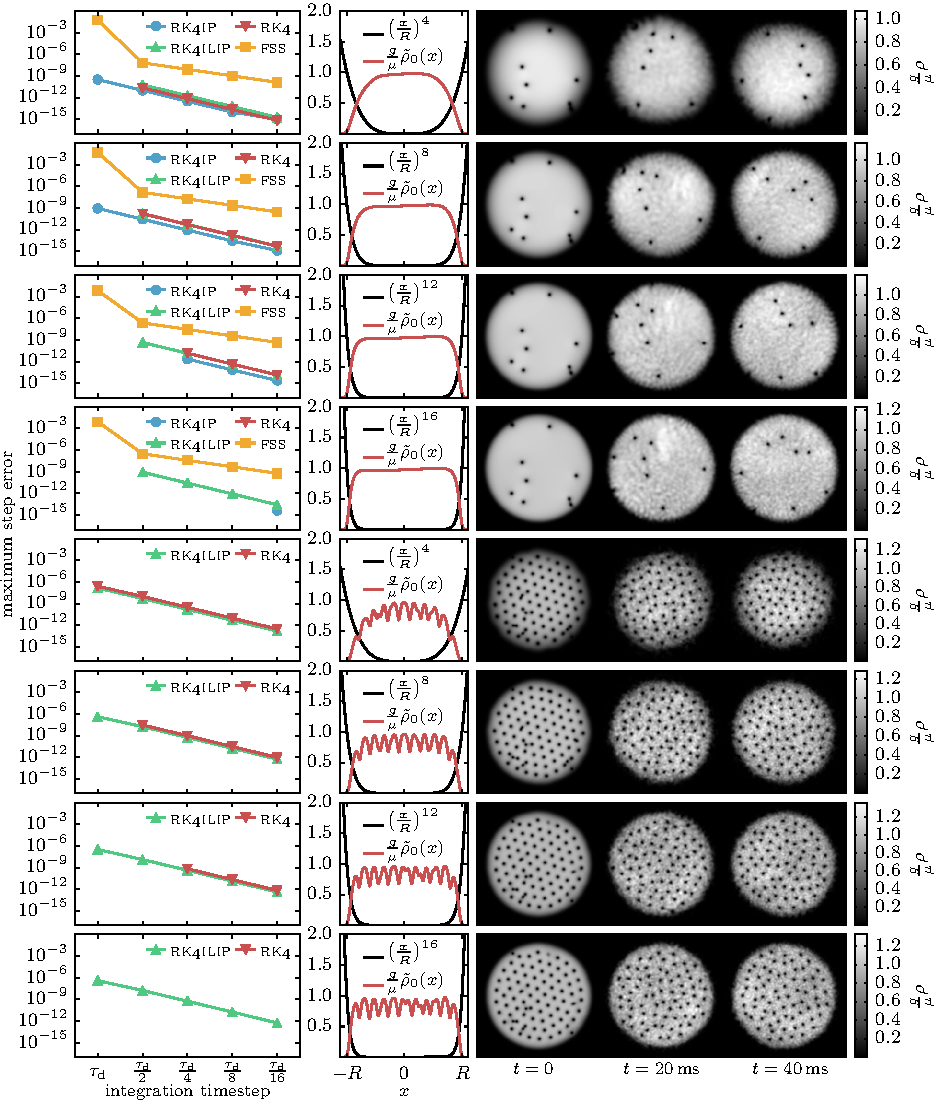
\includegraphics{figures/numerics/rk4ilip_results.pdf}
        \caption{Results of simulations to compare \textsc{rl4ilip} to other timestepping methods.
        Top four rows: Nonrotating frame simulations with four different radial power-law potentials.
        Bottom four rows: Rotating frame simulations with same four potentials.
        Left column: maximum per-step error $\int \abs{\psi - \tilde\psi}^2\,\dd \vec{r}/\int\abs{\tilde\psi}^2\,\dd \vec{r}$ of fourth order Runge--Kutta (\textsc{rk4}), its interaction picture variants (\textsc{rk4ip} and \textsc{rk4ilip}) and Fourier split-step (\textsc{fss}) as a function of timestep. Solutions were checked every $100$ timesteps against a comparison solution $\tilde \psi$ computed using half sized steps for \textsc{rk4} methods, and quarter sized steps for \textsc{fss}. Simulations encountering numerical overflow not plotted.
        Centre column: potential (black) and average density $\tilde \rho_0$ of the initial state  (red) over a slice of width $R/5$ in the $y$ direction.
        Right column: Density of solution at initial, intermediate and final times for each configuration simulated (taken from \textsc{rk4ilip} results).
        \textsc{rk4ilip} is the only method usable in rotating frames and not encountering overflow in the steeper traps for the timesteps considered.}
        \label{fig:rk4ilip_results}
    \end{figure}
    \restoregeometry
}

 Here I compare four numerical methods: Fourier split-step (\textsc{fss}), fourth order Runge--Kutta in the interaction picture (\textsc{rk4ip}), ordinary fourth order Runge--Kutta (\textsc{rk4}), and my new method --- fourth order Runge--Kutta in an instananeous local interaction picture (\textsc{rk4ilip}).

 The example chosen is a \textsc{2d} simulation of a turbulent Bose--Einstein condensate, in both a rotating and nonrotating frame. For the nonrotating frame the differential equation simulated was equation \eqref{eq:RK4_ILIP_GPE}, and for the rotating frame the same equation was with an additional two terms added to the Hamiltonian:
\begin{align}
\hat H_\up{rot} + \hat H_\up {comp} &= -\vec \Omega \cdot \hat{\vec L} +\frac12\hbar m^2\Omega^2 r^2\\
                &= \ii\hbar\Omega \left(x\pdv{y} - y\pdv{x}\right) +\frac12\hbar m^2\Omega^2 r^2.
\end{align}
The addition of the first term transforms the original Hamiltonian into a frame rotating at angular frequency $\Omega$ in the $(x, y)$ plane, and is equivalent to the the Coriolis and centrifugal forces that appear in rotating frames in classical mechanics \cite{Gulshani1978}. The second term is a harmonic potential that exactly compensates for the centrifugal part of this force. In this way the only potential in the rotating frame is the applied trapping potential, and the only effect of the rotating frame is to add the Coriolis force.

 Four trapping potentials were used, all radial power laws with different powers. These examples were chosen to demonstrate the specific situation in which \textsc{rk4ilip} provides a benefit over the other methods for spatial Schr\"odinger-like equations, as discussed above.

The results of $120$ simulation runs are shown in \figref{fig:rk4ilip_results}. Each simulation was of a $\ ^\up{87}$Rb condensate in the $\ket{F=2, m_F=2}$ state, in which the two-body $s$-wave scattering length is $a = 98.98$ Bohr radii \cite{vanKempen2002}. The simulation region was $20\unit{\mu m}$ in the $x$ and $y$ directions, and the Thomas--Fermi radius of the condensate was $R = 9\unit{\mu m}$.  The chemical potential was $\mu = 2\pi\hbar\times 1.91\unit{kHz}$, which is equivalent to a maximum Thomas--Fermi density $\rho_\up{max} = 2.5\E{14}\unit{cm}^{-3}$ and a healing length $\xi = 1.1\unit{\mu m}$. There were $256$ simulation grid points in each spatial dimension, which is $14$ points per healing length.

Four different potentials were used, all of the form $V(r) = \mu \left(r/R\right)^\alpha$ with $\alpha = 4, 8, 12, 16$. For the rotating frame simulations, the rotation frequency was $\Omega = 2\pi \times 148\unit{Hz}$. This is $89\%$ of the effective harmonic trap frequency, defined as the frequency of a harmonic trap that would have the same Thomas--Fermi radius given the same chemical potential.

All ground states were determined using successive over-relaxation (See section [TODO]) with sixth-order finite differences for spatial derivatives. For the nonrotating simulations, convergence was reached with $\upDelta\mu/\mu < 1\E{-13}$, with:
\begin{equation}
\upDelta\mu = \sqrt{\frac{\matrixel{\psi} {(\hat H - \mu)^2}{\psi}}{\braket {\psi}{\psi}}},
\end{equation}
where $\hat H$ is the nonlinear Hamiltonian and $\braket{\vec r}{\psi}$ is the condensate wavefunction, which does not have unit norm. For the rotating frame simulations the ground states converged to $\upDelta\mu/\mu \approx 9\E{-7}, 2\E{-6}, 3\E{-6}$ and $2\E{-6}$ for $\alpha = 16, 12, 8$, and $4$ respectively.

After each ground state was found, it was multiplied by a spatially varying phase factor corresponding to the phase pattern of a number of randomly positioned vortices:
\begin{align}
\psi_\up{vortices}(x, y) = \psi_\up{ground state}(x, y)\prod_{n=1}^N e^{\pm_n i\arctantwo(y - y_n, x - x_n)}
\end{align}
where $\arctantwo$ is the two-argument $\arctan$ function,\footnote{Defined as the principle value of the argument of the complex number $x + iy$: \mbox{$\arctantwo(y, x) = \Arg(x + iy)$.}} $N=30$, $\pm_n$ is a randomly chosen sign, and $(x_n, y_n)$ are vortex positions randomly drawn from a Gaussian distribution centred on $(0,0)$ with standard deviation equal to the Thomas--Fermi radius $R$. The same seed was used for the pseudorandom number generator in each simulation run, and so the vortex positions were identical in each simulation run.

After vortex phase imprinting, the wavefunctions were evolved in imaginary time \cite{chiofalo2000}. For the nonrotating frame simulations, imaginary time evolution was performed for a time interval equal to the chemical potential timescale $\tau_\mu= 2\pi\hbar/\mu$, and for the rotating frame simulations, for $\tau_\mu/10$. This was done to smooth out the condensate density in the vicinity of vortices, producing the correct density profile for vortex cores. However, since imaginary time evolution decreases the energy of the state indiscriminately, it also had the side effect of causing vortices of opposite sign to move closer together and annihilate. This decreased the number of vortices, and is the reason the smoothing step in the rotating frame simulations was cut short to $\tau_\mu/10$, as otherwise all vortices had time to annihilate with one of the lattice vortices. A vortex pair in the process of annihilating is visible in \figref{fig:rk4ilip_results} as a partially filled hole in the initial density profile near the top of the condensate in the $\alpha=4, 12,$ and $16$ rotating frame simulations.\footnote{The initial states for the four different potentials are not identical, so by chance the corresponding vortex in the $\alpha=8$ case was not close enough to a lattice vortex to annihilate.}

The smoothed, vortex imprinted states were then evolved in time for $40\unit{ms}$. For each simulation, five different timesteps were used: $\upDelta t = \tau_\up d, \tau_\up d / 2, \tau_\up d / 4, \tau_\up d / 8, \tau_\up d / 16$, where \mbox{$\tau_\up d = m \upDelta x^2 / \pi\hbar \approx 2.68\unit{\mu s}$} is the dispersion timescale associated with the grid spacing $\upDelta x$, defined as the time taken to move one gridpoint at the group velocity of the Nyquist mode.

For the nonrotating frame simulations, spatial derivatives for the \textsc{rk4} and \textsc{rk4ilip} methods were determined using the Fourier method [see section TODO]. This was to ensure a fair comparison with the other two methods, which necessarily use Fourier transforms to perform computations pertaining due to the kinetic term.

For the rotating frame simulations, sixth-order finite differences with zero boundary conditions were used instead for the kinetic terms of the \textsc{rk4} and \textsc{rk4ilip} methods, which were the only two methods used for those simulations (due to the other methods being incompatible with the angular momentum operator required for a rotating frame). This choice was fairly arbitrary, but did allow the condensate to be closer to the boundary than is otherwise possible with the periodic boundary conditions imposed by use of the Fourier method for spatial derivatives. This is because the rotating frame Hamiltonian is not periodic in space, and so its discontinuity at the boundary can be a problem if the wavefunction is not sufficiently small there.

As shown in \figref{fig:rk4ilip_results}, all methods tested generally worked well until they didn't work at all, with the per-step error of \textsc{rk4}-based methods being either small and broadly the same as the other \textsc{rk4}-based methods, or growing rapidly to the point of numerical overflow (shown as missing datapoints). The break down of \textsc{fss} was less dramatic, though it too had a clear jump in its per-step error for larger timesteps. Comparing methods therefore came down to mostly whether or not a simulation experienced numerical overflow during the time interval being simulated.

The main result was that \textsc{rk4ilip} and \textsc{fss} remained accurate over the widest range of timesteps and trap steepnesses, with \textsc{rk4} and \textsc{rk4ip} requiring ever smaller timesteps in order to not overflow as the trap steepness increased.

For the rotating frame simulations, which were only amenable to the \textsc{rk4} and \textsc{rk4ilip} methods, the same pattern was observed, with \textsc{rk4} only working at smaller timesteps as the trap steepness was increased, and ultimately diverging for all timesteps tested at the maximum trap steepness. By contrast, \textsc{rk4ilip} remained accurate over the entire range of timesteps at the maximum trap steepness.

\subsection{Discussion}

As mentioned, \textsc{rk4ilip} is mostly useful for continuum quantum mechanics only when there are large spatial differences in the potential, which cannot give rise to equally large kinetic energies\footnote{This is essentially due to such a situation violating the condition we laid out at the beginning of this section --- that the simulation basis must be nearly an eigenbasis of the total Hamiltonian.}. Furthermore, the advantage that \textsc{rk4ilip} has over other methods with that same property is that it is does not require a particular form of Hamiltonian or a particular method of evaluating spatial derivatives. The former means it is applicable in rotating frames or to situations with unusual Hamiltonians, and the latter means is can be used with finite differences or \textsc{fedvr} \cite{schneider_parallel_2006} and thus is amenable to parallelisation on a cluster computer.

The ability to model large spatial variations in the potential provides only a narrow domain of increased usefulness over other methods. If a large kinetic energy results from the large potential, then the method requires just as small timesteps as any other. And if the large potential is supposed to approximate an an infinite well, then an actual infinite well may be modelled using zero boundary conditions, negating the need for something like \textsc{rk4ilip}. However, when potential wells are steep, but not infinitely steep, here \textsc{rk4ilip} provides a benefit. The only other model that can handle these large potentials---Fourier split-step---has the disadvantage that it cannot deal with arbitrary operators such as those arising from a rotating frame, and is not parallelisable with local data. The benefits of parallelisability are obvious, and the above results demonstrate \textsc{rk4ilip}'s advantage at simulating \textsc{bec}s in tight traps and rotating frames.

Note that whilst the \emph{Fourier} split-step method can't handle Hamiltonian terms such as $\hat {\vec r} \cdot \hat {\vec p}$ that are not diagonal in either real space or Fourier space \cite[p.~315]{tannor_introduction_2007}, a split-step method based on an approximation to the momentum operator as a banded matrix, such as that obtained with finite differences, can. Using the techniques discussed in section \ref{sec:split-step-parallel}, such a scheme is also parallelisable. The remaining limitations then, when compared to fourth-order Runge--Kutta are the restriction on the types of nonlinearity that can be included, and the complexity of implementation.

For systems with discrete degrees of freedom, \textsc{rk4ilip} may be useful in the case where an approximate diagonalisation of the Hamiltonian is analytically known, and when the Hamiltonian's eigenvalues vary considerably in time (making a single interaction picture insufficient to factor out dynamical phases throughout the entire simulation). In this situation an analytic transformation into the diagonal basis can be performed at each timestep (or the differential equation analytically re-cast in that basis in the first place), and \textsc{rk4ilip} can be used to factor out the time-varying dynamical phase evolution at each timestep. An example may be an atom with a magnetic moment in a time-varying magnetic field which varies over orders of magnitude. The transformation into the spin basis in the direction of the magnetic field can be analytically performed, and if the field varies by orders of magnitude, so do the eigenvalues of the Hamiltonian. Although the eigenvalues in this case and other similar cases can be computed analytically too, unless all time dependence of the Hamiltonian is known in advance of the simulation, it would be difficult to incorporate this into a re-casting of the differential equation in a time-dependent interaction picture. \textsc{rk4ilip} may be useful in these cases to automate this process and evolve the system in the appropriate interaction picture at each timestep.


% \setcounter{chapter}{3}
% \chapter{Software for experiment control and analysis}\label{chap:software}

\includepdf[pages=2-]{labscript_paper/labscript_paper.pdf}


% \setcounter{chapter}{4}
% 
\chapter{Particle velocimetry of vortices in Bose–Einstein condensates}\label{chap:velocimetry}

\lettrine[lines=3]{T}{his chapter investigates}, via numerical simulation, an imaging method for the real time tracking of quantum vortices in a turbulent $^{41}$K condensate. The method involves ultracold $^{87}$Rb tracer particles that become bound to vortex lines in the condensate and are imaged continuously to track the vortex lines as they move. The imaging of tracer particles to track vortex motion has previously proved successful in superfluid helium~\cite{bewley_generation_2009, bewley_superfluid_2006, packard_vortex_1982}, and the method of laser cooling and imaging atoms in high resolution with the same laser light has also been successful in cold atom systems~\cite{bakr_quantum_2009}. This chapter presents the results of numerical simulations of the method under a number of assumptions to establish its feasibility as an imaging method. 

\begin{figure}
\begin{center}
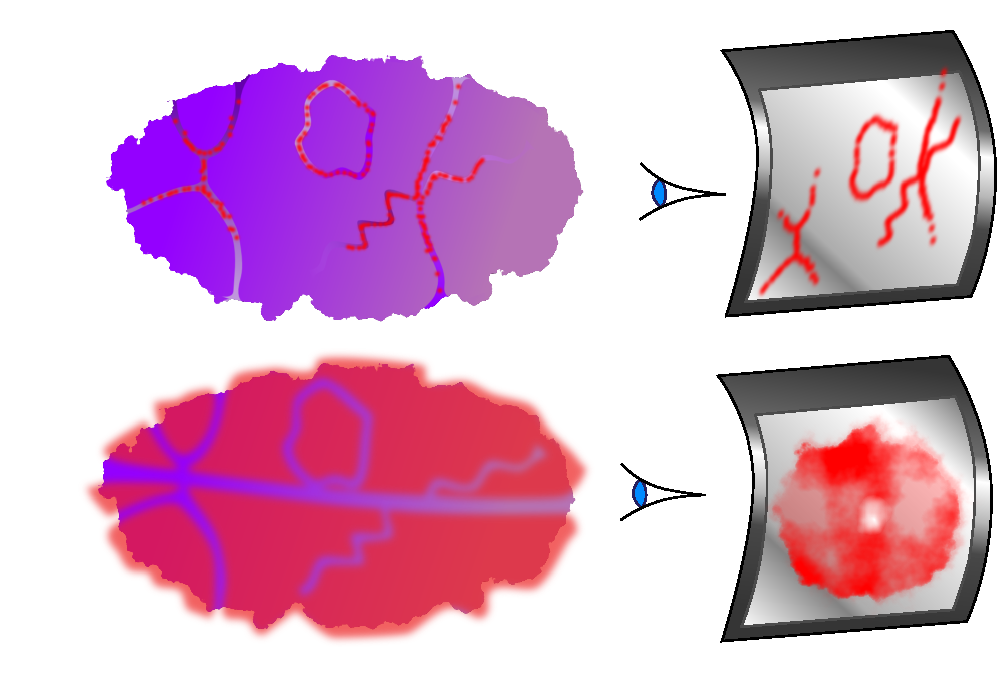
\includegraphics[width=0.6\textwidth]{figures/unsorted/side-on.pdf}
\caption{\label{fig:side-on}Imaging of the condensate itself, whether by flourescence (bottom) or absorption imaging makes it difficult to resolve vortices unless they are viewed end-on. The vortex cores are usually smaller than the imaging light's wavelength, and are thus also difficult to resolve unless the cloud is allowed to expand. Imaging tracer particles instead (top) has the potential to resolve both these problems.}\label{fig:side_on}
\end{center}
\end{figure}

This method has the potential to overcome several existing difficulties that typical imaging techniques face when used to image vortices. In ordinary absorption imaging, atoms are imaged via resonant absorption of the condensate itself, and vortices---visible as density minima---generally can only be seen when the vortex line is normal to the image plane. If not viewed end-on in this way, a vortex line represents only a minor decrease in column density and cannot be distinguished from the rest of the condensate (\figref{fig:side_on}). One solution to this problem is to slice the condensate into layers, and image them separately~\cite{anderson_watching_2001}.

The use of tracer particles that are only present within vortex cores allows vortex lines to be visible from any viewing angle.  Furthermore, since the atoms being imaged reside in the vortex cores themselves rather than the bulk of the condensate, this imaging can potentially be repeatedly or continuously performed without destroying the condensate. This may enable observation of the time evolution of Kelvin waves~\cite{bretin_quadrupole_2003}, vortex reconnections~\cite{leadbeater_sound_2001}, and vortex rings~\cite{anderson_watching_2001}.

This \emph{in-situ} imaging of vortex dynamics may allow more types of vortex motion to be imaged. Dynamics of \bec s are typically studied using a shot-by-shot method, in which repeated experiments with identical initial conditions are imaged destructively after being allowed to evolve for different amounts of time. Whilst this works for many types of dynamics, it fails for experiments that are sensitive to initial conditions and noise (quantum or otherwise), such as turbulent flow. This includes phenomena which cannot be created reliably in the same initial state, even though the evolution thereafter would be consistent from one experimental run to the next. One such phenomenon is the spontaneous generation of vortices after evaporative cooling~\cite{weiler_spontaneous_2008}.

\emph{In-situ} imaging of vortex motion has been achieved previously~\cite{freilich_real-time_2010}, by ejecting a fraction of the atoms from the condensate periodically and imaging them. This process is limited by depletion of the condensate, and was also used only to image vortices end-on. The fraction of the condensate being imaged was also allowed to freely expand before being imaged, since vortex cores are otherwise unable to be resolved by the wavelength of light used. Our proposed method would require neither free expansion or depletion of the condensate.

\section{Motivation: Turbulence}

It is commonly said that turbulence is one of the greatest unsolved problems of classical physics. But in what sense is it an unsolved problem? It is not a problem at all if your aim is reductionism---the Navier--Stokes equation adequately describes the evolution of a Newtonian fluid within its domain of validity, and the process of deriving it from the underlying motion of classical particles is well understood. It's turtles all the way down~\cite[p 1]{hawking_brief_1988}; what more could we ask for?

A demonstrative comparison might be with the field of thermodynamics, as precisely the same statement can be made about the energy content and exchange between systems of particles. Thermodynamics has revealed that despite the chaotic motion of individual particles in an ensemble, definite statements can still be made about the behaviour of the system as a whole, \emph{without having to consider the dynamics of the constituent components in detail}.

This is the kind of solution people have in mind when they speak of `solving' the problem of turbulence. Laws describing the average properties of a fluid without reference to its precise flow field would not simply be interesting as describing turbulence as an emergent phenomenon, but would aid practical computations, which for many problems of interest are prohibitively computationally expensive. The flow of a turbulent fluid contains detail on such a  wide range of length scales that finite-element or finite-difference analyses of a system such as an aeroplane wing requires a very high resolution in order to be accurate. Following an estimate of computing power required to simulate a turbulent system down to its smallest length scales, Stanley Corrsin quipped~\cite{corrsin_turbulent_1961}:
\begin{quote}
The foregoing estimate  is enough to suggest the use of analog instead of digital  computation; in particular, how about an analog consisting of a tank of water?
\end{quote}
The reliance of the aerospace industry on wind tunnels and practical tests shows that there is some truth to the necessity of using nature as one's computer when it comes to turbulence. Whilst nature must always have the final say, it would be of great benefit to be able to compute expected results more cheaply before setting up a wind-tunnel experiment or constructing a prototype aircraft.

But are we asking for too much? Perhaps the statistical properties of a turbulent fluid fundamentally cannot be decoupled from the finer details. There is reason to believe that this is not the case. There are several tantalising results that hint at universal properties that all turbulent flows share, and there is the simple empirical observation that the average flow of turbulent fluids at large scales is reproducible from one experimental run to the next~\cite[pp 13, 86]{davidson_turbulence:_2004}.

One of these universal results is Kolmogorov's theory of the statistics of small eddies~\cite{kolmogorov_local_1941, spalding_kolmogorovs_1991}. Another is the fact that the rate of energy dissipation via the action of viscosity at small scales is independent of the viscosity itself~\cite[p 77]{davidson_turbulence:_2004}.

Then there is the Richardson energy cascade~\cite{richardson_weather_2007}, in which energy is continually transferred from larger scales to smaller scales. With dissipation at the smallest scales and addition at larger scales, this allows for the existence of `steady state' turbulence.

The above examples derive from ordinary, viscous fluids. Bose--Einstein condensates on the other hand are superfluids. There are several interesting aspects of superfluid turbulence that differ from classical turbulence. The defining difference is the absence of viscosity; another major difference is the quantisation of circulation. On length scales much larger than spacing between vortex lines, superfluid turbulence is expected to closely resemble classical turbulence~\cite{tsubota_energy_2009}. At smaller scales however the energy dissipation mechanism is different, instead involving the production of sound waves via vortex interactions~\cite{tsubota_energy_2009, vinen_how_2005}.

In certain 2\textsc{d} geometries, an \emph{inverse cascade}~\cite{onsager_statistical_1949, kraichnan_inertial_1967} is predicted to take place in superfluids, whereby energy moves not from large scales to small, but from small to large, clustering quantised vortices of the same circulation direction together. This phenomenon has been studied theoretically and numerically in the Monash Quantum Fluids group~\cite{simula_emergence_2014, groszek_vortex_2018} and recently experimentally observed in the Monash Dual-Species laboratory in experiments performed by Shaun Johnstone~\cite{johnstone_order_2018}, simultaneously with a group at the University of Queensland~\cite{gauthier_negative-temperature_2018}.

The following definition of turbulence, taken from~\cite[p 53]{davidson_turbulence:_2004}, emphasises the role of vortices in turbulence in general:
\begin{quote}
Incompressible hydrodynamic turbulence is a spatially complex distribution of vorticity which advects itself in a chaotic manner in accordance with [the vorticity equation\footnote{Which is a transformation of the Navier--Stokes equation for an incompressible fluid into a form in which the vorticity field is center-stage.}]. The vorticity field is random in both space and time, and exhibits a wide and continuous distribution of length and time scales.
\end{quote}

When vorticity exists only in infinitely narrow lines, as it does in superfluid, the vorticity equation mentioned in the above definition reduces to a Biot--Savart type law which can be used to compute the motion of vortices without having to compute the entire flow field.

This is why we are interested in the study of the dynamics of quantised vortices. Unlike in classical fluids, the vortices in superfluids have a definite position and size; there is either a vortex at a given spatial location or there is not. This may make it simpler to describe the motion of vortices statistically.

So far experimental studies of superfluid turbulence have been primarily in the context of liquid helium~\cite{leggett_superfluidity_1999}. Bose--Einstein condensates offer a compelling alternative subject of study for superfluid turbulence. The high degree of control afforded over systems of cold atoms allows the superfluid's properties to be tweaked in several ways, creating a larger parameter space in which to study turbulence than that afforded by liquid helium.

\section{Overview of velocimetry scheme}

\begin{figure}
\begin{center}
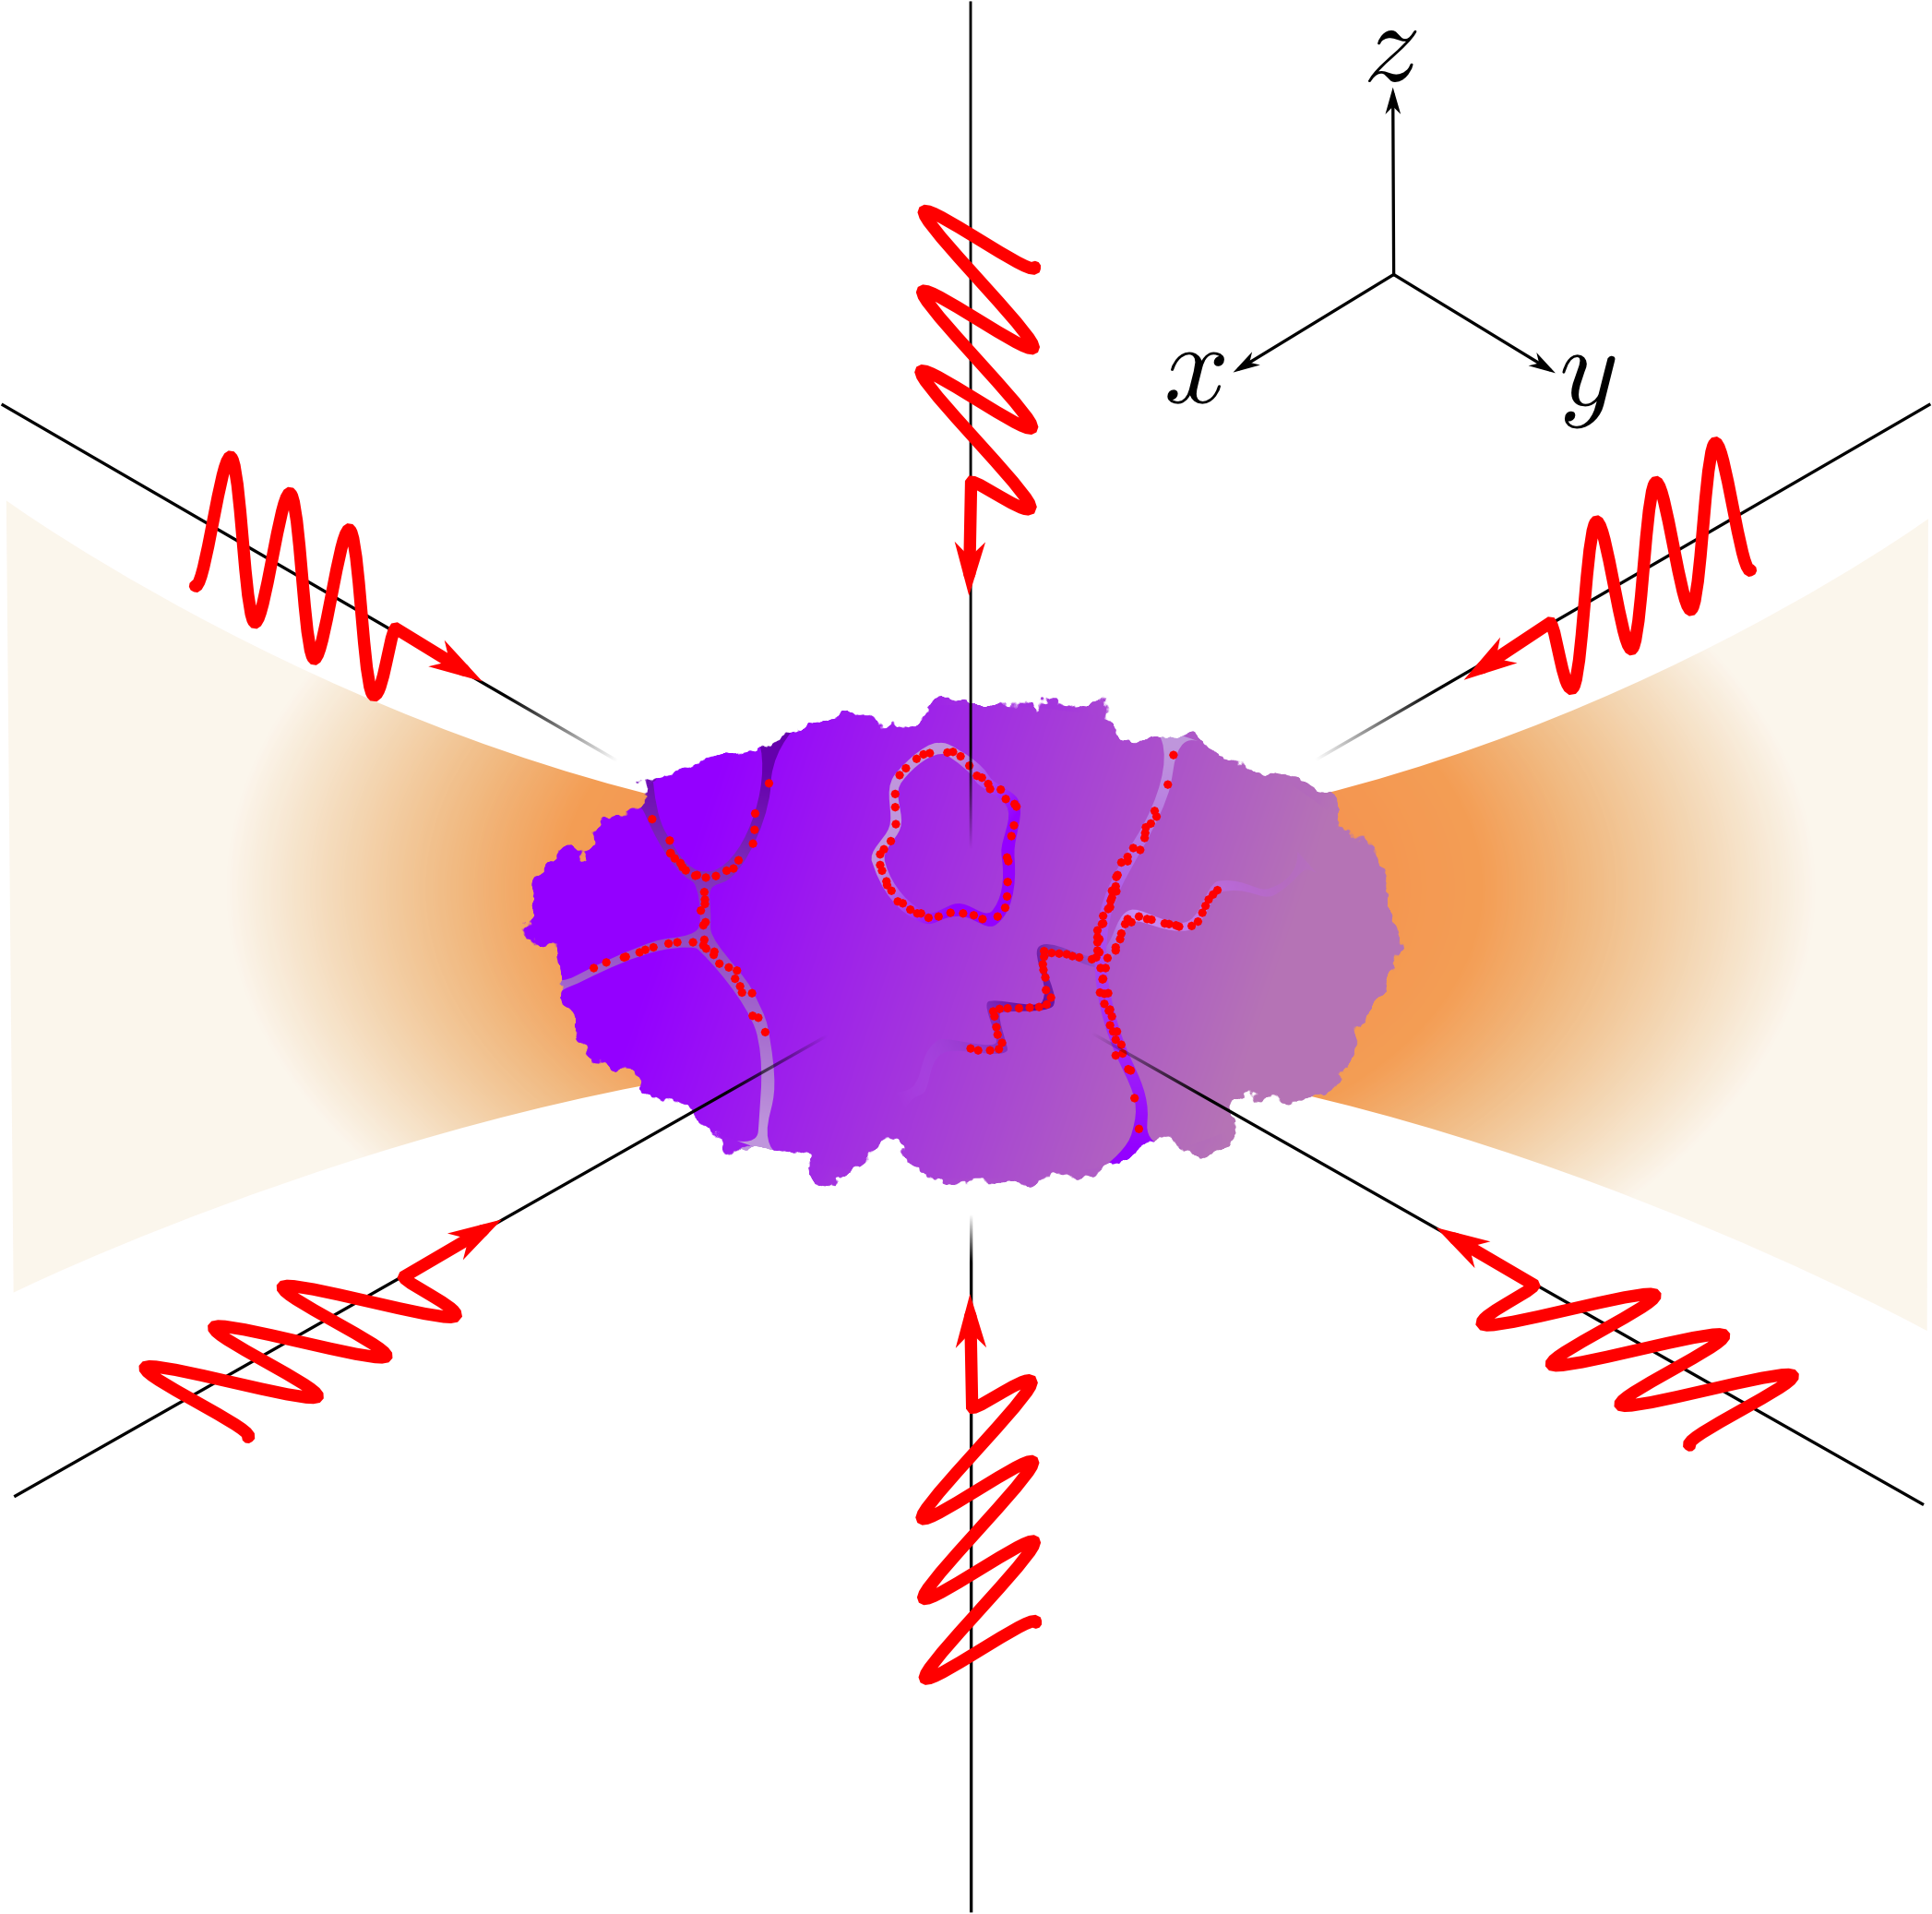
\includegraphics[width=0.6\textwidth]{figures/unsorted/setup.png}
\caption{\label{fig:setup}The simplest scheme for cooling and imaging the tracer particles with the same light is polarisation gradient cooling, involving six slightly off resonant beams (red), with each counterpropagating pair having opposite linear polarisations. This will scatter some light off the tracer atoms, as well as cool them to sub-Doppler temperatures. If the cooling is sufficient, it should encourage the atoms into the vortex cores where their energy is lower, if they aren't already there. Both the rubidium tracers and the potassium \bec\ will be trapped with approximately the same trapping potential by a strong, far off-resonant laser (orange), via the dipole force. Magnetic trapping cannot be used, as polarisation gradient cooling does not work in the presence of a magnetic field.}
\end{center}
\end{figure}

As mentioned, the core idea of our proposed imaging method is to use tracer particles to track vortex cores in a \bec\ in real time. In this chapter I consider $^{87}$Rb atoms as tracer particles in a \textsc{bec} made of $^{41}$K. This choice is due to the strong interspecies repulsion between these atomic species, which gives rise to the trapping of atoms in the vortex cores. In the limit of low densities and temperatures, such that three body collisions are suppressed and $s$-wave scattering dominates the interspecies interactions~\cite[p 120]{leggett_quantum_2006}, the rubidium tracer atoms experience a potential due to the potassium:

\begin{equation}
V(\vec{r}) = \frac{2\pi\hbar^2 a_s}{m_r}\rho_\up{K}(\vec{r}),
\end{equation}
where $\rho_\up{K}(\vec{r})$ is the spatially varying atom density of the potassium condensate, $a_s$ is the interspecies $s$-wave scattering length, and
$m_r = \frac{m_\up{K}m_\up{Rb}}{m_\up{K} + m_\up{Rb}}$ is the reduced mass of the scattering pair. Vortex cores thus create potential wells for other atoms, since they are regions of low condensate density in a background of high density.

The basic setup of the scheme is shown in Figure~\ref{fig:setup}. Cold rubidium atoms are introduced (such as by magnetic transport from a \mot) to a potassium condensate, after which both species are optically trapped at the focus of a high power $1064$nm laser, using the dipole force. Various methods may be used to create vortices in the condensate. These include bluff-body flow, where a repulsive potential is dragged through the condensate, and inducing a turbulent state by applying off-resonant laser speckle. The rubidium atoms are then expected to become trapped in the low density vortex cores.

The atoms are imaged with resonant or near-resonant laser light, depending on the exact scheme employed. In this chapter I present the results of simulating two configurations, one of which has near-resonant laser light also cooling the atoms to keep them trapped in the vortex cores, and the other relying solely on sympathetic cooling with imaging being performed with resonant light.

The simplest scheme which attempts to cool the rubidium atoms is ordinary polarisation gradient cooling, in which the same light is used for imaging and cooling the atoms (Figure~\ref{fig:setup}). This was considered in my Honours thesis~\cite{billington_particle_2010}, the results of which I summarise in the next section. This method precludes the use of a magnetic trap or large bias field, since either would destroy the cooling effect.

The vortex potentials may be made deeper through the use of a Feshbach resonance (Section~\ref{sec:feshbach}), which increases the interspecies scattering length. However, since this requires a magnetic field, it precludes the use of ordinary polarisation gradient cooling. In section (see Section~\ref{sec:laser_cooling_simulations}) I present an alternative polarisation gradient cooling scheme designed work in the presence of a magnetic field of the strength required for the Feshbach resonance of interest.

Effective imaging of vortex motion would require approximately $10^5$ photons per second to scatter off each rubidium atom without it escaping its vortex core trap, and without causing so much heating as to destroy the condensate on a reasonable experimental timescale. A high resolution, low aberration lens (numerical aperture $\approx 0.5$) would also be required to focus the scattered light onto a fast capture, high quantum efficiency camera to produce images of vortex motion.

\section{Relation to previous work}

This scheme was first investigated in my Honours project~\cite{billington_particle_2010}. In that work I investigated the ability of vortex potentials to trap atoms, including consideration of the depth of such traps when measured in units of the photon recoil energy. Considering the depth in these units was a first attempt to estimate how easily atoms may escape vortex potentials in the presence of imaging light. Figure~\ref{fig:levels1e14} and Figure~\ref{fig:levels1e15}show bound states of typical vortex potentials at different condensate densities.

\begin{figure}
\centering
\noindent\makebox[\textwidth]{
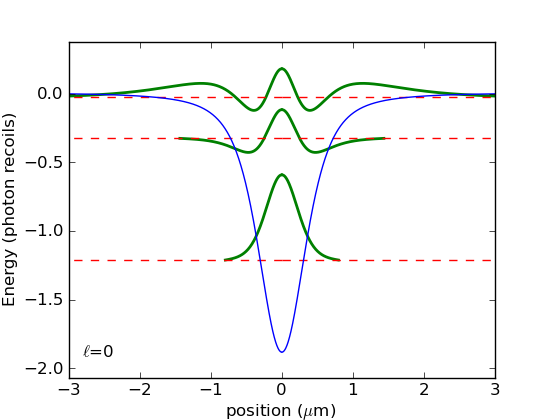
\includegraphics[width=0.5\columnwidth]{figures/velocimetry/levels1e14_l=00.png}
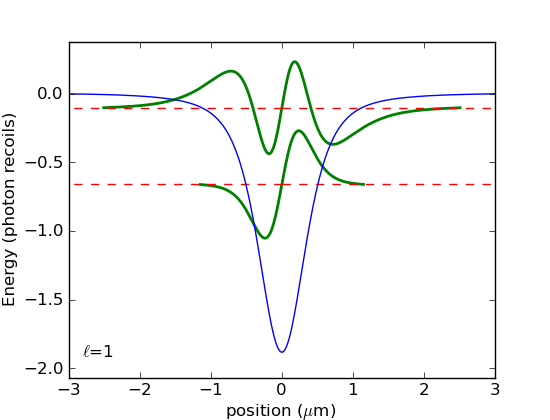
\includegraphics[width=0.5\columnwidth]{figures/velocimetry/levels1e14_l=01.png}}
\noindent\makebox[\textwidth]{
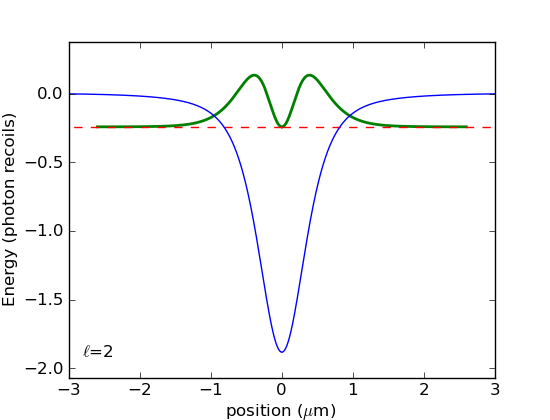
\includegraphics[width=0.5\columnwidth]{figures/velocimetry/levels1e14_l=02.png}
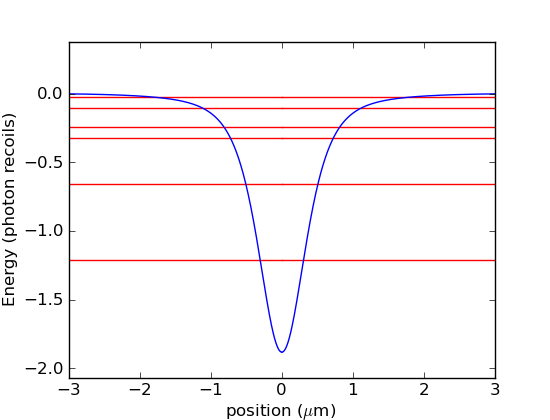
\includegraphics[width=0.5\columnwidth]{figures/velocimetry/levels1e14.png}}
\caption{Energy eigenstates of a rubidium atom in a potassium vortex core, for a potassium \textsc{bec} with background density $\approx 10^{14}\unit{cm}^{-3}$. There are a number of bound states spanning three orbital quantum numbers. Plots of the bound states are of a cross section through the centre of a vortex core, and the lower right plot shows just the energy levels. Figure reproduced from~\cite{billington_particle_2010}.}%
\label{fig:levels1e14}%
\end{figure}

\begin{figure}
\centering
\noindent\makebox[\textwidth]{
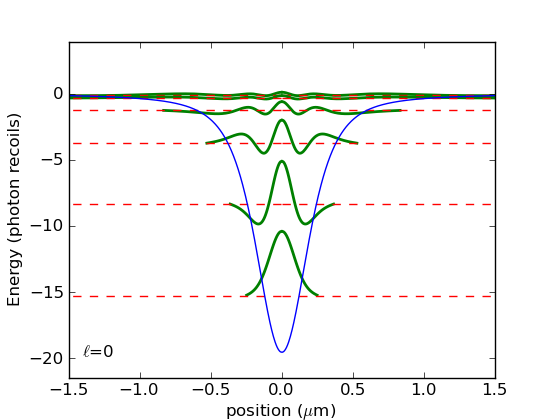
\includegraphics[width=0.5\columnwidth]{figures/velocimetry/levels1e15_l=00.png}
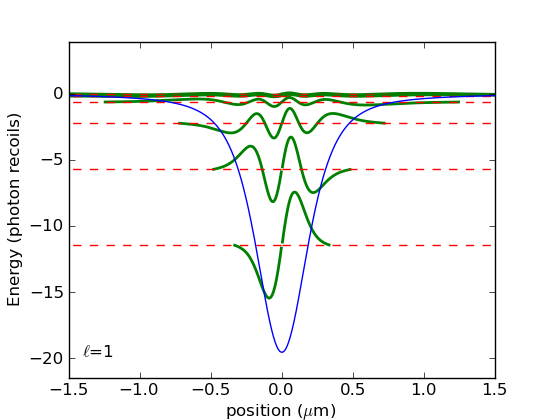
\includegraphics[width=0.5\columnwidth]{figures/velocimetry/levels1e15_l=01.png}}
\noindent\makebox[\textwidth]{
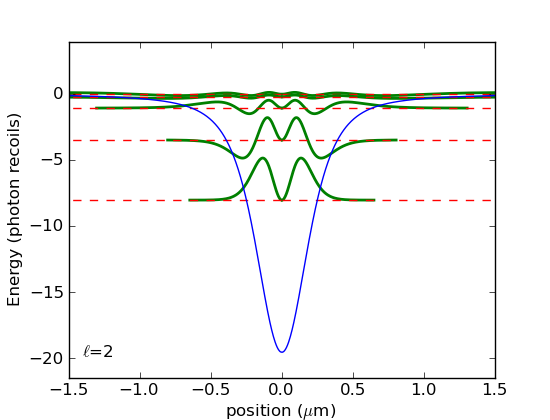
\includegraphics[width=0.5\columnwidth]{figures/velocimetry/levels1e15_l=02.png}
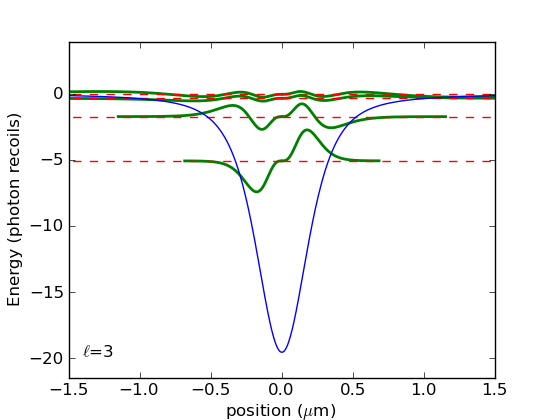
\includegraphics[width=0.5\columnwidth]{figures/velocimetry/levels1e15_l=03.png}}
\noindent\makebox[\textwidth]{
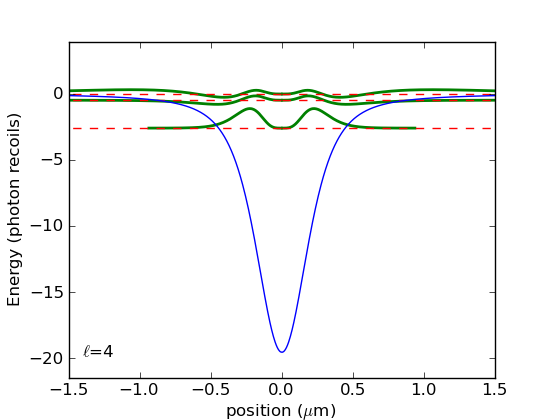
\includegraphics[width=0.5\columnwidth]{figures/velocimetry/levels1e15_l=04.png}
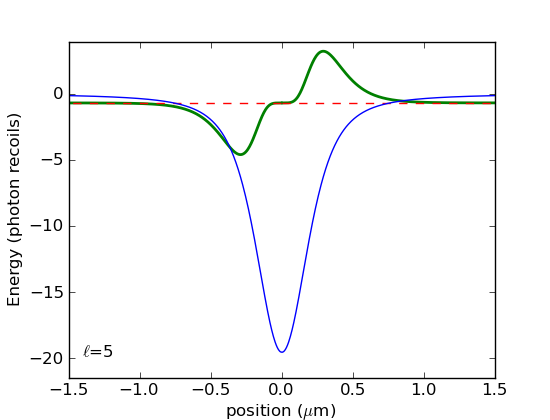
\includegraphics[width=0.5\columnwidth]{figures/velocimetry/levels1e15_l=05}}
\noindent\makebox[\textwidth]{
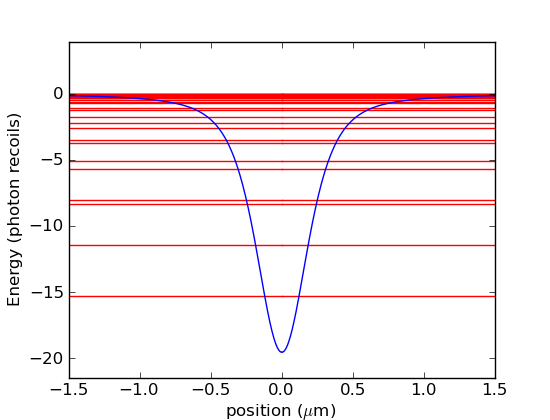
\includegraphics[width=0.5\columnwidth]{figures/velocimetry/levels1e15.png}}
\caption{As in Figure~\ref{fig:levels1e14}, but for a potassium \textsc{bec} with background density ${\approx 10^{15}\unit{cm}^{-3}}$. There are bound states over six different orbital quantum numbers. This vortex potential is much deeper than that in Figure~\ref{fig:levels1e14}, showing the effect of condensate density on the depth of the vortex potentials. Figure reproduced from~\cite{billington_particle_2010}.}%
\label{fig:levels1e15}%
\end{figure}

There were a number of conclusions from this investigation. Firstly, to minimise the recoil energy, rubidium is a better choice for tracer particle than potassium due to its larger mass, enabling a rubidium atom to remain trapped after scattering a number of photons that would cause a potassium atom to escape the same potential. Secondly, vortex potentials are not very deep when measured in recoil energies, and their depth depends strongly on the density of the \textsc{bec}. At typical condensate densities of $10^{14}\unit{cm}^{-3}$, the vortex potentials are expected to only be one or two recoil energies deep, making it unlikely that atoms could scatter many photons whilst remaining trapped in them. At larger densities of $10^{15}\unit{cm}^{-3}$, the vortex potentials are closer to $20$ recoil energies deep, making imaging of trapped tracer atoms more plausible.

The main simulation result of my Honours project considered a potassium condensate with a peak density of $10^{15}\unit{cm}^{-3}$ and rubidium tracer atoms being cooled using standard polarisation gradient cooling with parameters chosen to ensure each atom scattered $10^5$ photons per second in two spatial dimensions. The result was that initially randomly distributed rubidium atoms were able to become and remain trapped in the vortex cores whilst being cooled (Figure~\ref{fig:hybrid}).

\begin{figure}
\centering
\noindent\makebox[\textwidth]{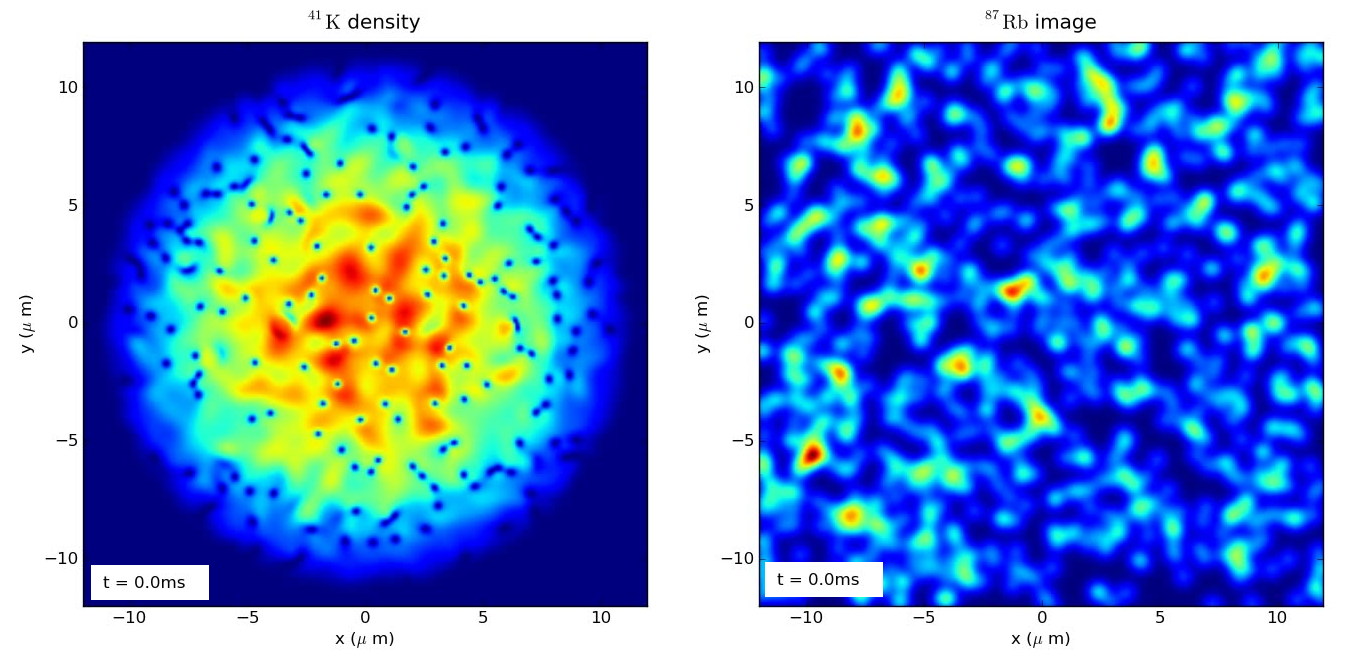
\includegraphics[width=1.0\columnwidth]{figures/velocimetry/hybrid1.png}}
\noindent\makebox[\textwidth]{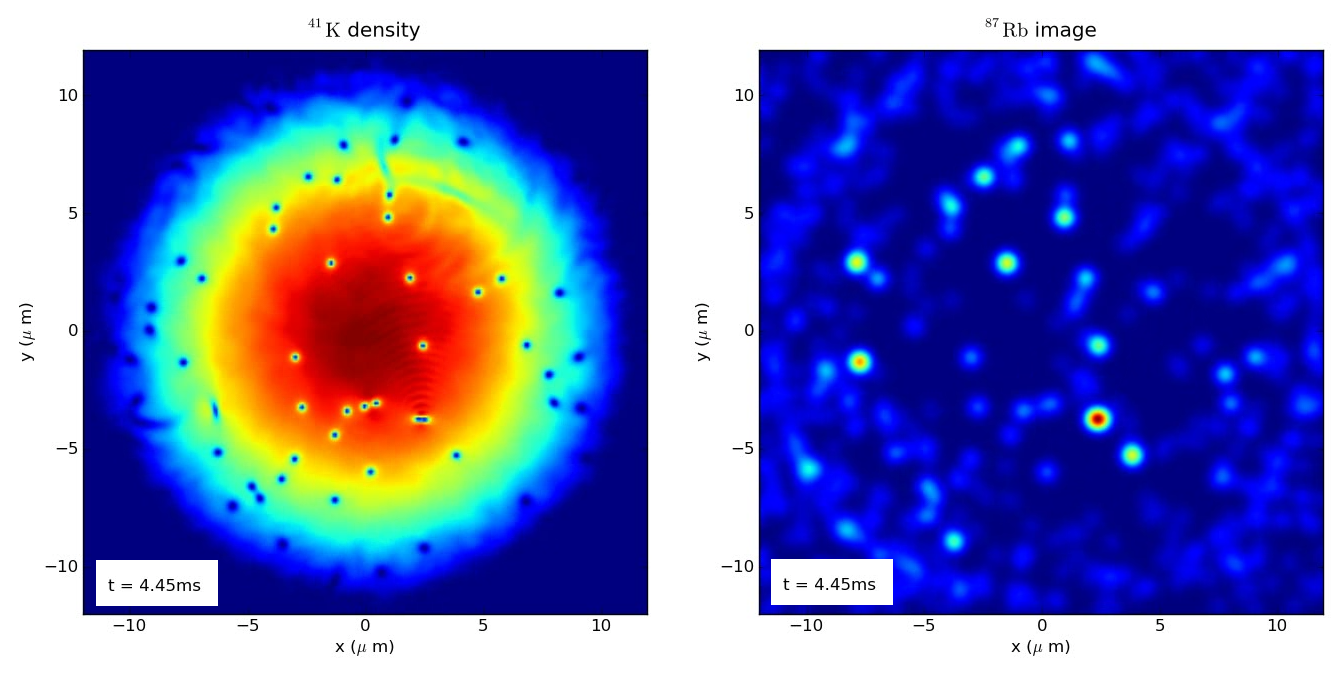
\includegraphics[width=1.0\columnwidth]{figures/velocimetry/hybrid2.png}}
\noindent\makebox[\textwidth]{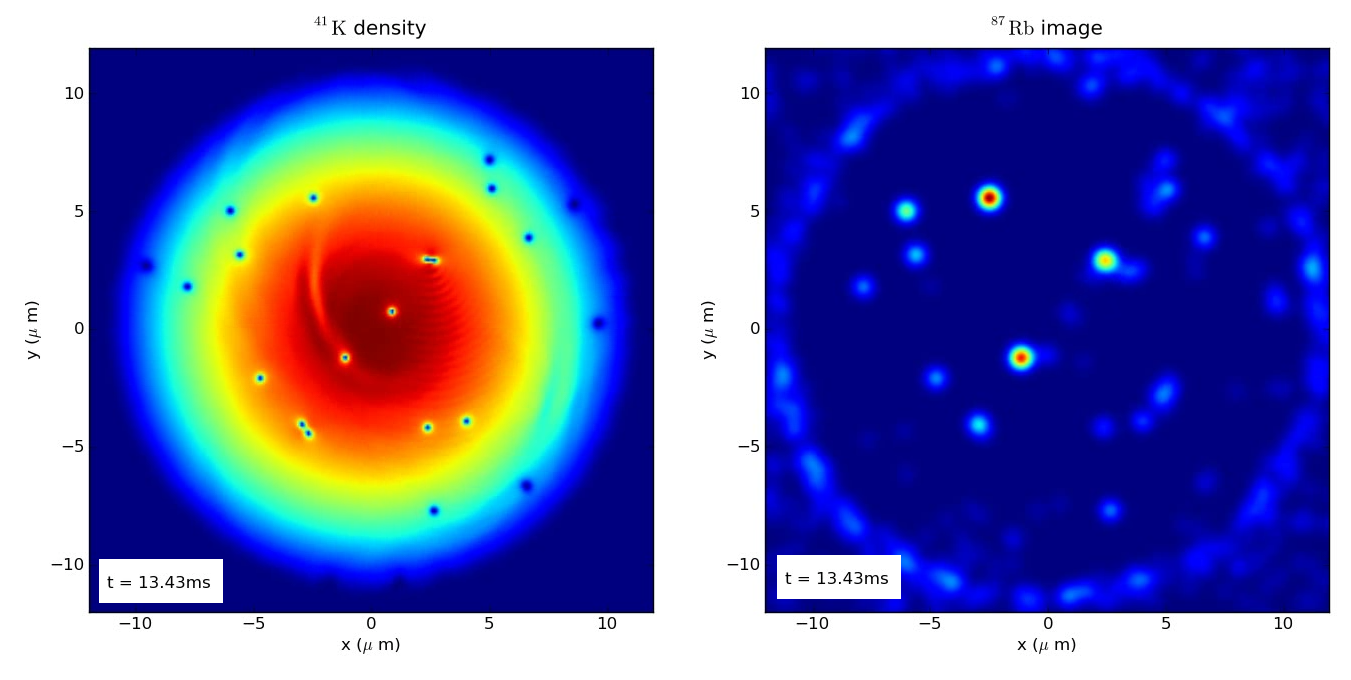
\includegraphics[width=1.0\columnwidth]{figures/velocimetry/hybrid3.png}}
\caption{The result from~\cite{billington_particle_2010} of a two-dimensional hybrid quantum-classical simulation for 1000 classical rubidium atoms (right, depicted as fluorescence assuming diffraction through an $\mathrm{NA}=0.5$ imaging system) and a turbulent potassium \textsc{bec} (left) of peak density $\approx 10^{15}\unit{cm}^{-3}$. The rubidium atoms are subject to a classical approximation of the force due to polarisation gradient cooling as described in~\cite{billington_particle_2010}. Most rubidium atoms eventually either become bound to a vortex core or leave the condensate. Figure reproduced from~\cite{billington_particle_2010}.}%
\label{fig:hybrid}%
\end{figure}

However, the density assumed in this simulation was rather high for a real experiment. Three-body losses tend to limit the lifetime of condensates at such a high density, and so the work in this chapter investigates ways to make particle velocimetry work in a less dense condensate. As the vortex potentials are so shallow at lower density, as mentioned earlier the potentials may be deepened through the use of a Feshbach resonance.

In Section~\ref{sec:sympathetic} I consider a similar configuration, but with a more reasonable \textsc{bec} density combined with an enhancement of the interspecies repulsion due to a Feshbach resonance. I investigate whether sympathetic cooling of the tracer atoms by the condensate may be enough to keep them trapped in the presence of imaging light. Then, in Section~\ref{sec:laser_cooling_simulations} I present simulation results of a new laser cooling scheme designed to work at the magnetic field strength required for the Feshbach resonance.

\section{Sympathetic cooling}\label{sec:sympathetic}

The simulation performed in my Honours thesis considered only polarisation gradient cooling counteracting the heating effect of the imaging light. In reality, collisions between tracer atoms and atoms in the condensate would also contribute to cooling. This sympathetic cooling of the tracer atoms---which would also lead to heating of the condensate---was disregarded in my Honours thesis' results. 

Depending on the strength of the cooling effect from sympathetic cooling, this cooling may be sufficient to retain tracer atoms in vortex cores in the absence of an additional cooling mechanism such as polarisation gradient cooling. If laser cooling is not necessary to trap tracer atoms in vortices, then the Feshbach resonance may be used to enhance the interspecies scattering length, further enhancing the ability of the vortices to trap tracer atoms. In this section I consider a similar simulation to that in my Honours thesis, in which the tracer atoms are subject to sympathetic cooling only, in order to examine this possibility.

\subsection{Model}

In this section I model sympathetic cooling due to elastic two-body scattering between the rubidium tracer atoms and the potassium atoms in the condensate. The model is two-dimensional, approximating a pancake-shaped condensate. As with the simulation in my Honours thesis, I model the \textsc{bec} with the damped Gross--Pitaevskii equation:
\begin{align}
\ii\hbar\pdv{t} \Psi_\up{K}(\vec r, t) = (1-\ii\gamma)\left[-\frac{\hbar^2}{2m_\up{K}}\nabla^2 + V(\vec{\vec r}) + g_\up{K}\abs{\Psi_\up{K}(\vec r, t)}^2\right]\Psi_\up{K}(\vec r, t),
\end{align}
with damping constant $\gamma=0.01$ and all other symbols are as defined in Section~\ref{sec:mean_field_theory}, with the added subscripts $_\up{K}$ indicating quantities specific to $^{41}\up{K}$. The $^{41}$K $s$-wave scattering length is $a_\up{K}=121 a_0$~\cite{cote_potassium_1998}, where $a_0$ is the Bohr radius. The damped \textsc{gpe}~\cite{tsubota_vortex_2002, madarassy_vortex_2008} is a phenomenological modification of the standard \textsc{gpe} that includes dissipation which gradually removes higher energy excitations from the condensate wavefunction, a finite temperature effect. The condensate wavefunction is normalised at each timestep. The potential $V(\vec r)$ is a harmonic potential:
\begin{align}
V(\vec r) = \frac12m_\up{K}\omega_\up{K}^2 r^2
\end{align}
where $\omega_\up{K}=2\pi\times 130\unit{Hz}$.
The rubidium tracer atoms are modelled classically, evolving under the potential due to interspecies repulsion, as well as the external potential\footnote{For simplicity I assume that both species are subject to the same external potential. Written as a harmonic trap for rubidium such that $V(\vec r) = \frac12m_\up{K}\omega_\up{K}^2 r^2 = \frac12m_\up{Rb}\omega_\up{Rb}^2 r^2$ gives $\omega_\up{Rb}= 2\pi\times 90\unit{Hz}$.} $V(\vec r)$, resulting in the equation of motion:
\begin{align}\label{eq:classical_motion_tracers}
\dv[2]{t} \vec r = -\frac1{m_\up{Rb}}\nabla\left({g_{\textrm{Rb--K}}} \abs{\Psi_\up{K}(\vec r, t)}^2 + V(\vec r)\right),
\end{align}
where $g_{\textrm{Rb--K}}$ is the $^{87}$Rb--$^{41}$K non-linear interaction constant
\begin{align}
g_{\textrm{Rb--K}} = \frac{2\pi\hbar^2 a_{\textrm{Rb--K}}}{m_\up{r}},
\end{align}
where $m_\up{r}$ is the reduced mass of the $^{87}$Rb--$^{41}$K scattering pair and 
$a_{\textrm{Rb--K}}$ is the $s$-wave interspecies scattering length, equal to $640 a_0$ at zero magnetic field~\cite{thalhammer_double_2008}, and assumed in this section to be enhanced by a factor of five by means of the $34\unit{G}$ Feshbach resonance (see Section~\ref{sec:feshbach} and \figref{fig:feshKRb}). Since the Gross--Pitaevskii equation is solved on a grid whereas the classical motion of the atoms is modelled using continuous position variables, the condensate density is numerically differentiated and the results interpolated to the positions of the tracer atoms using cubic splines in order to evaluate~\eqref{eq:classical_motion_tracers} for each tracer atom.

The motion of the tracer atoms is punctuated by velocity jumps due to both the scattering of imaging photons and two-body collisions with the condensate. Photon scattering events are modelled as instantaneous velocity jumps of magnitude $v_\up{r} = hc/\lambda m_\up{Rb}$ where $\lambda=780\unit{nm}$ is the wavelength of the imaging light. A random direction in \textsc{3d} space is chosen and a velocity jump in this direction with the given magnitude is projected into the \textsc{2d} plane of the simulation before being applied to the atom. These jumps occur at random times at an average rate given by the target photon scattering rate. 

Collisions with the condensate are modelled as elastic collisions between a rubidium atom with the given classical velocity, and a potassium atom of velocity equal to the superfluid velocity $\vec v_\up{K}$ of the condensate (discussed in Section~\ref{sec:mean_field_theory}) at the location of the tracer atom, given by
\begin{align}
\vec v_\up{K}(\vec r, t) = \frac \hbar {m_\up{K}} \nabla \phi_\up{K}(\vec r, t),
\end{align}
where $\phi_\up{K}(\vec r, t)$ is the complex phase of the potassium condensate wavefunction. The $s$-wave scattering length $a$ is defined as~\cite[p 589, eq.~12.101]{bransden_physics_2003}
\begin{align}
a = -\lim_{k_\up{rel}\rightarrow 0} \frac{\tan\left(\delta_0(k_\up{rel})\right)}{k_\up{rel}},
\end{align}
where $k_\up{rel}=m_\up{r}v_\up{rel}/\hbar$ is the relative wavenumber of the colliding pair of atoms with reduced mass $m_\up{r}$ and relative velocity $v_\up{rel}$, and $\delta_0(k)$ the collisional phase shift. Assuming small $k_\up{rel}$ and substituting this into the $s$-wave elastic scattering cross section~\cite[p 584, eq.~12.66]{bransden_physics_2003} 
\begin{align}
\sigma = \frac{4\pi}{k_\up{rel}^2}\sin^2\left(\delta_0(k_\up{rel})\right)
\end{align}
gives a low-velocity approximation to the scattering cross section for elastic collisions between the rubidium and potassium atoms:
\begin{align}\label{eq:sigma_scattering}
\sigma_{\textrm{Rb--K}} \approx 4\pi\frac{a_{\textrm{Rb--K}}^2}{1 + k_\up{rel}^2a_{\textrm{Rb--K}}^2}.
\end{align}
For rubidium atoms at $5\unit{\upmu K}$, $k_\up{rel}a_{\textrm{Rb--K}} < 0.1$, such that the zero-velocity scattering cross section $\sigma = 4\pi a^2$ would be accurate enough; nonetheless~\eqref{eq:sigma_scattering} is the expression used in this section.\footnote{For modestly larger Feshbach enhancements of the scattering length, the zero-velocity cross section would not be accurate and the velocity dependence of the scattering cross section would become important.} From the scattering cross section we obtain the mean free path of a rubidium tracer particle within the potassium \textsc{bec}:
\begin{align}
\ell(\vec r, t) = \left(\sigma_{\textrm{Rb--K}}\abs{\Psi_\up{K}(\vec r, t)}^2\right)^{-1},
\end{align}
yielding the probability of a collision occurring in an infinitesimal time interval $\dd t$:
\begin{align}\label{eq:P_collision}
P_\up{collision}(\vec r, t+\dd t, t) = v_\up{rel}(\vec r, t)\sigma_{\textrm{Rb--K}}\abs{\Psi_\up{K}(\vec r, t)}^2\dd t,
\end{align}
where $v_\up{rel} = \abs{\vec v_\up{K}(\vec r, t) - \vec v}$ for a specific rubidium atom at position $\vec r$ and with velocity $\vec v$.

At each timestep, a random number between zero and one is generated for each atom, and if less than~\eqref{eq:P_collision}, a collision is taken to have occurred.\footnote{During thesis writing, an error was discovered in the code that produced the results in this section, in which the computed collision probability~\eqref{eq:P_collision} was too small by a factor of $\sqrt{2}$. As such, the results shown in the next subsection underestimate the sympathetic cooling effect slightly. I do not expect this error to change any of my conclusions.} In the case of a collision, the \textsc{2d} elastic scattering problem is solved and the rubidium atom's velocity instantaneously replaced with its post-collision value. The potassium condensate wavefunction is not modified---the sympathetic heating resulting from these collisions is ignored, which is a limitation of these results.

\subsection{Results}

I simulated the equations described in the previous section in two dimensions, with the \textsc{gpe} solved on a $256\times256$ grid (representing a spatial region of $40\unit{\upmu m}\times40\unit{\upmu m}$) using fourth-order Runge--Kutta (Section~\ref{sec:rk4}) with $\upDelta t = 500\unit{ns}$ using fast Fourier transforms to evaluate the kinetic energy term (Section~\ref{sec:fourier_pseudospectral}), and the tracer atoms' equations of motion propagated also using fourth-order Runge--Kutta with the same timestep. $1\times10^3$ tracer atoms were simulated. The first derivatives of the condensate wavefunction required to compute its phase gradient were evaluated using second-order finite differences, which I observed to be less susceptible to Gibbs' phenomenon in the vicinity of vortex cores, which---when using Fourier transforms---would produce a velocity field with unphysical radial motion close to a vortex core.\footnote{Interestingly, second derivatives---as required for the kinetic energy term of the \textsc{gpe}---do not appear to suffer from this problem at similar grid resolutions.}

I computed the initial conditions for the condensate wavefunction using the imaginary time evolution method (Section~\ref{sec:ITEM}) subject to a fixed \textsc{2d} normalisation constant leading to a peak density of $4\times 10^{14}\unit{cm}^{-3}$. Once the groundstate condensate wavefunction was found, a turbulent state was constructed by imposing a phase pattern on the condensate on a $16\times16$ grid, with the phase in each region chosen randomly from the interval $(-\pi, \pi)$. The imaginary time evolution algorithm was then applied once more for $300\unit{\upmu s}$ to produce a physically realistic condensate wavefunction containing a number of vortices randomly distributed.

The initial conditions of the tracer atoms comprised random initial positions uniformly distributed over the entire spatial region, and velocities drawn from a Maxwell--Boltzmann distribution at $5\unit{\upmu K}$.

I these evolved these initial in time for $16\unit{ms}$ with sympathetic cooling being modelled, but with zero photon scattering (Figure~\ref{fig:velocimetry_dark}). This allowed many of the tracer atoms to either move into vortex cores or leave the condensate (those that left mostly moved in a ring at the Thomas--Fermi radius where the external potential and interspecies potential resulted in a potential minimum).

After this period of sympathetic cooling without imaging was simulated, I then evolved the system further in time with the addition of imaging light. This part of the simulation was run twice.

In the first imaging simulation, shown in Figure~\ref{fig:velocimetry_idealised}, the photon scattering rate was $1\times10^5$ photons per second and imaging proceeded for $6.6\unit{ms}$. The location of every photon emission event, binned to a $256\times256$ grid, was recorded to produce an image of the tracer particles' locations over the simulation. In this image, the paths of vortices are clearly visible in the motion of the tracer atoms, showing vortex motion and interaction.

However, this is an idealised situation. Assuming a numerical aperture of $0.5$ and unity quantum efficiency, only approximately $4.2\,\%$ of photons emitted would be detected by an imaging system; there would also be diffraction. To take these effects into account in a second run of the imaging part of the simulation, for each photon emission a random number was chosen to determine whether it was to be included in a simulated image with probability $0.042$. No attempt was made to choose photons based on their emission direction---which photons were included in the image was entirely random. The position of the photon on the image produced was then summed with a random number drawn from a Gaussian distribution with zero mean and standard deviation of $0.33\unit{\upmu m}$, which is a Gaussian approximation to the point spread function of a $\up{NA}=0.5$ imaging system. This produced an image that took into account finite collection efficiency and diffraction. I found that in order to be able to see vortex positions, a higher photon scattering rate was required. In Figure~\ref{fig:velocimetry_realistic} I show the results of this second run of the imaging part of the simulation, using a higher photon scattering rate of $5\times10^5$ photons per second. Due to the heating of the tracer atoms, a reduced imaging duration of only $2\unit{\upmu s}$ was used as after that the tracer atoms had mostly escaped the vortex cores. Vortices are still visible in these results, but their motion is not discernible. This suggests that as-is, sympathetic cooling may be enough to image vortex positions with brief imaging pulses, but may not be sufficient to track them over time unless a larger scattering length enhancement via a Feshbach resonance is used, or unless additional cooling can be provided.


\afterpage{
    \newgeometry{left=1in,bottom=1.5in,right=1in,top=1.5in}
    \begin{sidewaysfigure}[th]
    \centerfloat
    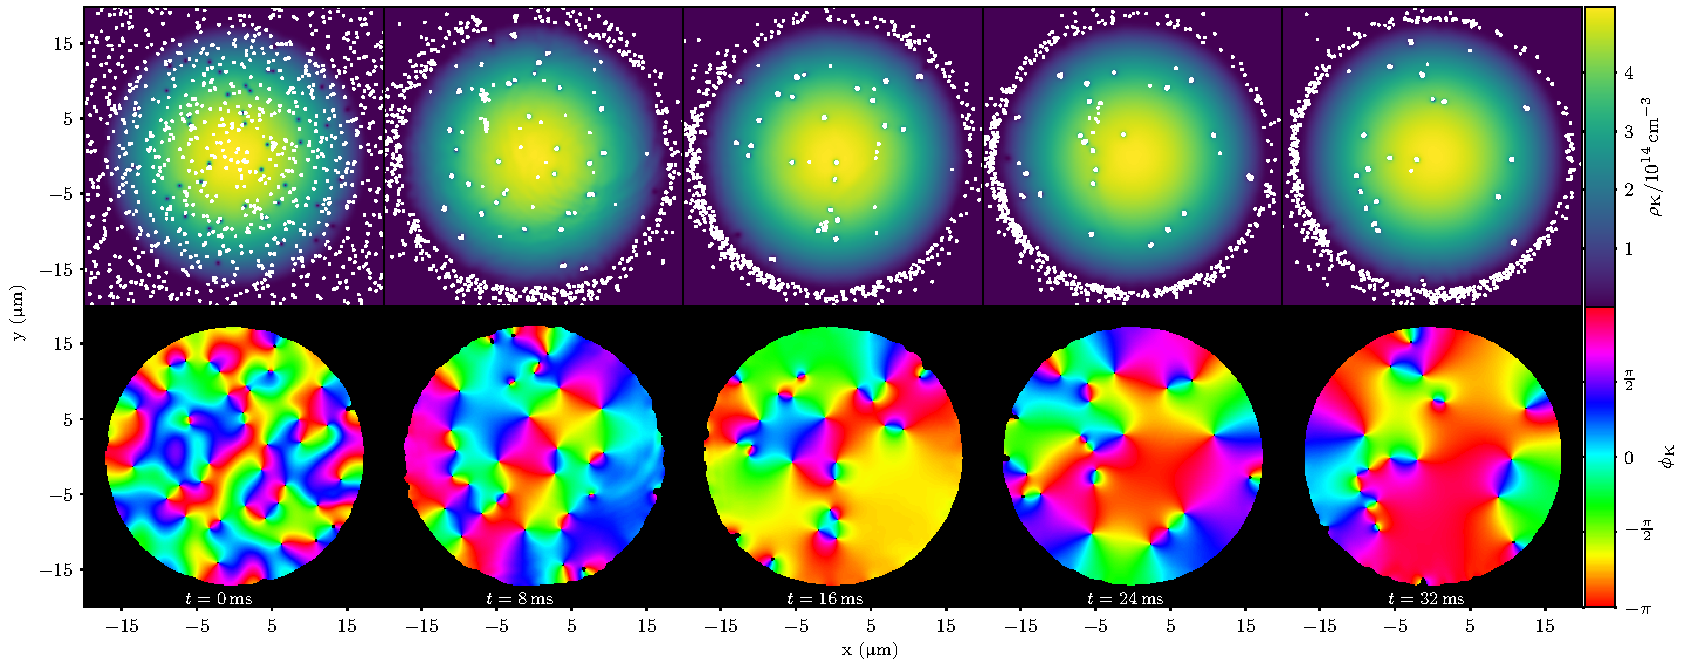
\includegraphics[width=1.05\textwidth]{figures/velocimetry/evolution_high_density.pdf}
    \caption{caption}
    \label{fig:evolution_high_density}
    \end{sidewaysfigure}
    \restoregeometry
}

\clearpage

\begin{figure}
\begin{center}
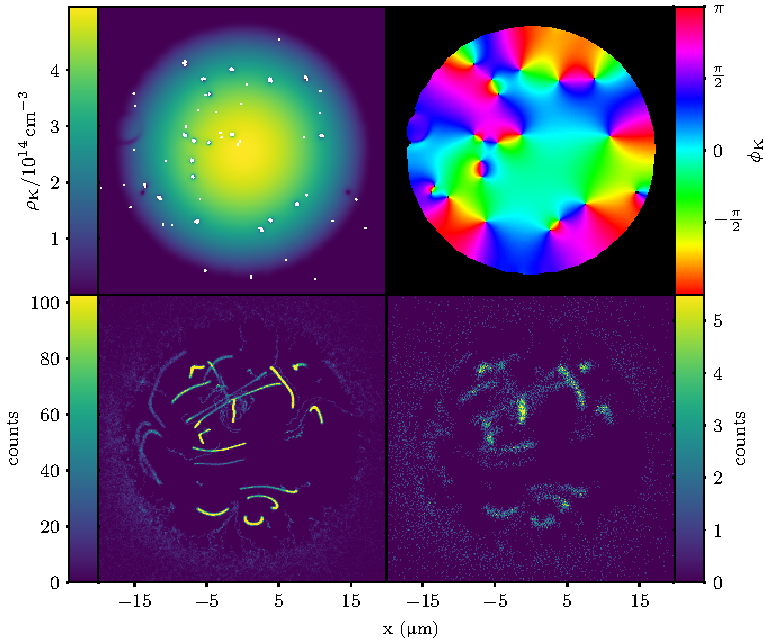
\includegraphics[width=\textwidth]{figures/velocimetry/imaging_high_densitynormal_start.pdf}
\caption{Caption}\label{fig:imaging_high_densitynormal_start}
\end{center}
\end{figure}

\begin{figure}
\begin{center}
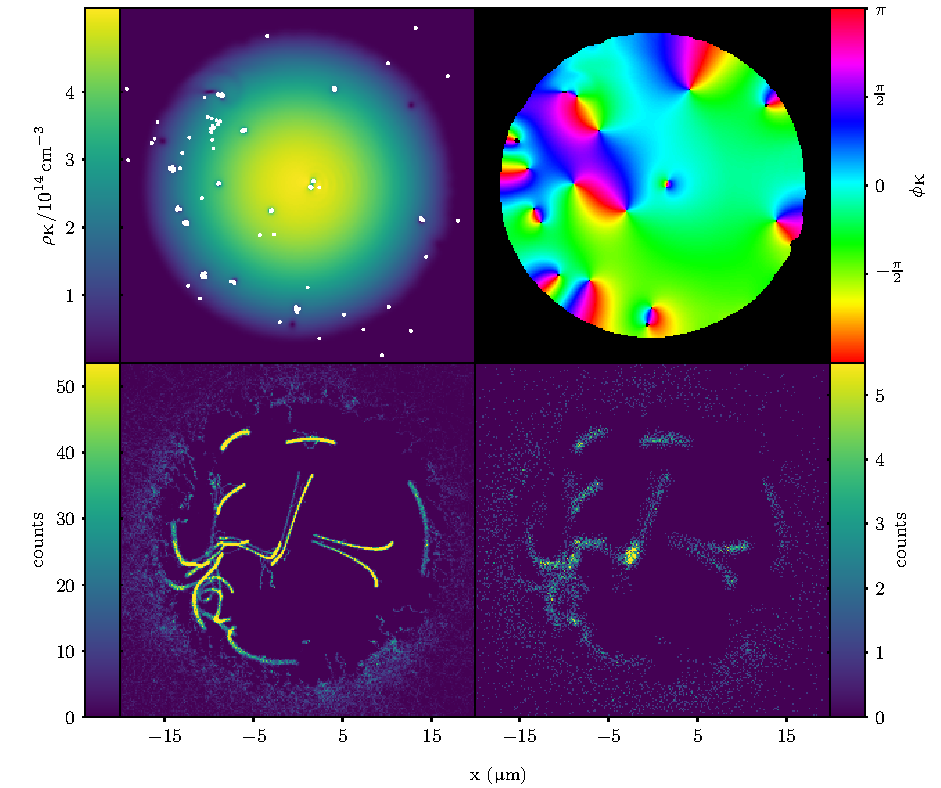
\includegraphics[width=\textwidth]{figures/velocimetry/imaging_high_densitylate_start.pdf}
\caption{Caption}\label{fig:imaging_high_densitylate_start}
\end{center}
\end{figure}



\afterpage{
    \newgeometry{left=1in,bottom=1.5in,right=1in,top=1.5in}
    \begin{sidewaysfigure}[th]
    \centerfloat
    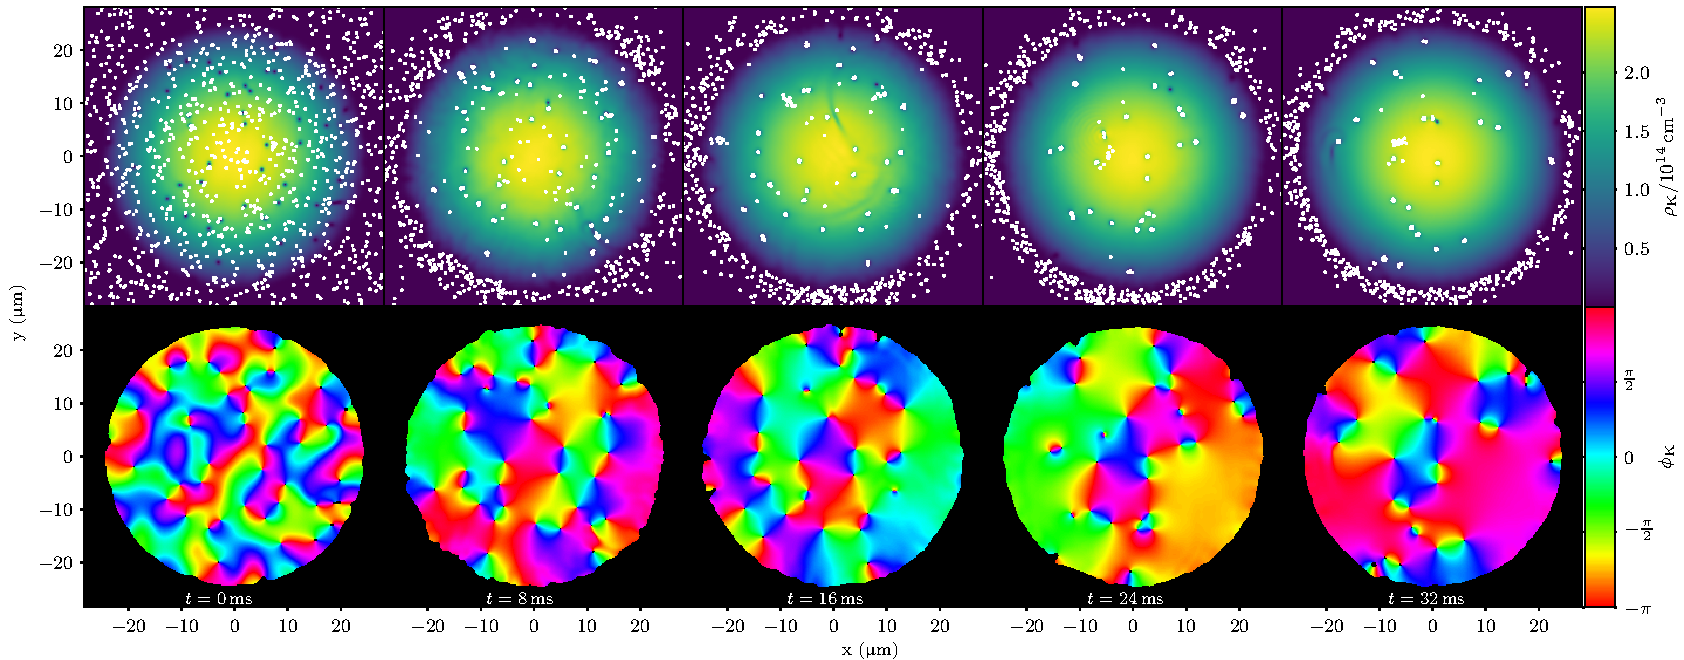
\includegraphics[width=1.05\textwidth]{figures/velocimetry/evolution_low_density.pdf}
    \caption{caption}
    \label{fig:evolution_low_density}
    \end{sidewaysfigure}
    \restoregeometry
}

\clearpage

\begin{figure}
\begin{center}
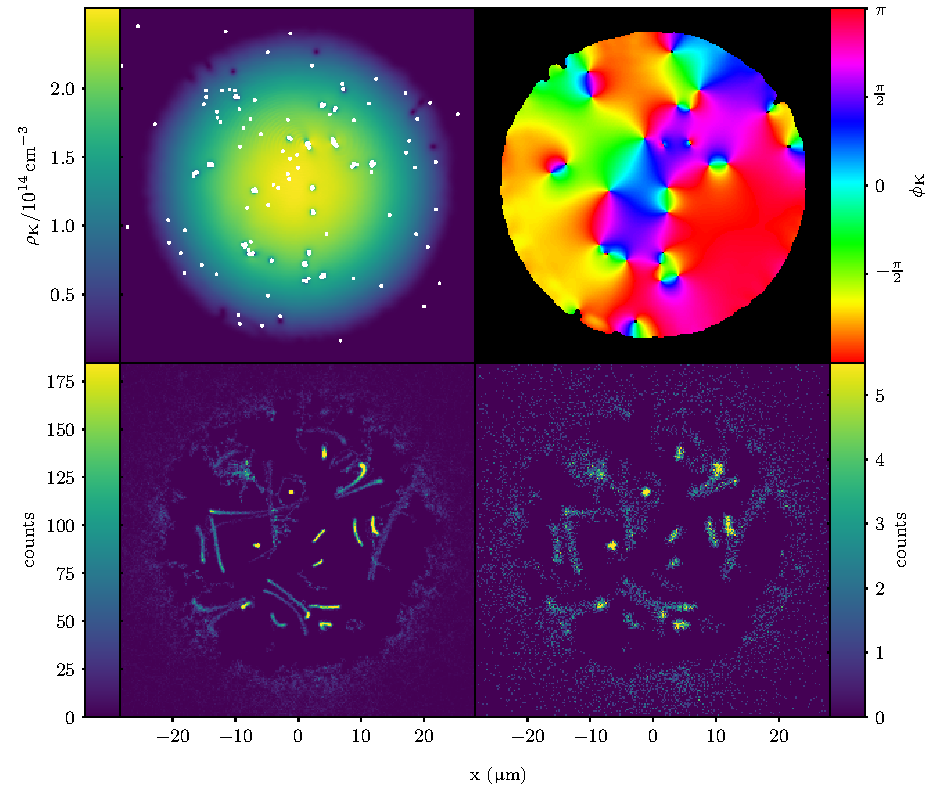
\includegraphics[width=\textwidth]{figures/velocimetry/imaging_low_densitynormal_start.pdf}
\caption{Caption}\label{fig:imaging_low_densitynormal_start}
\end{center}
\end{figure}

\begin{figure}
\begin{center}
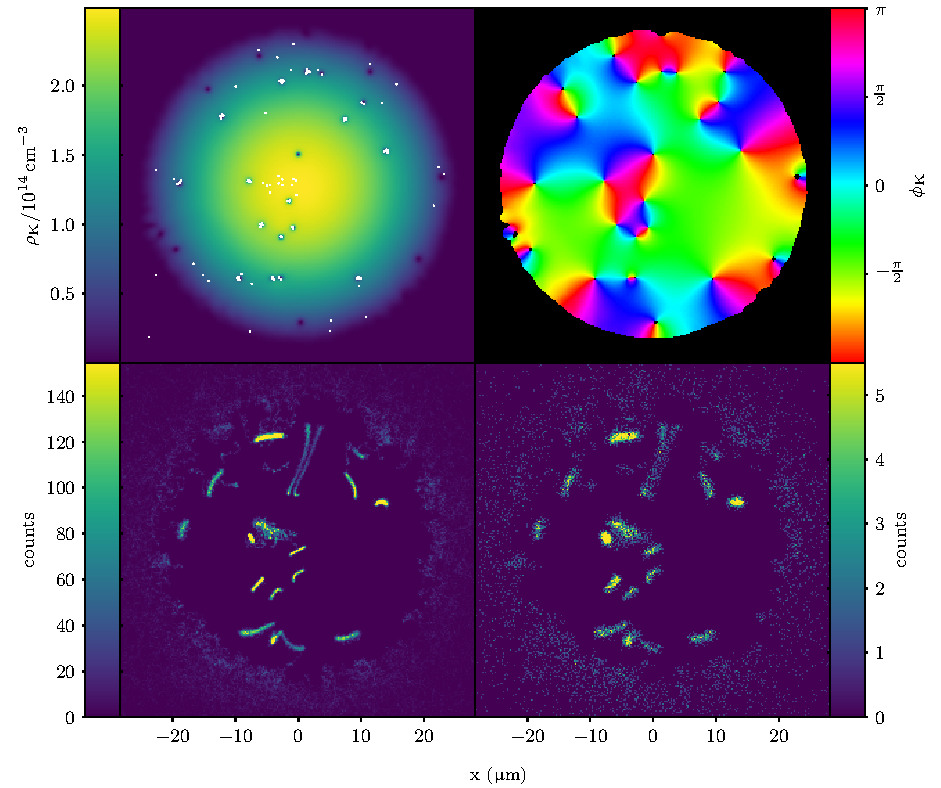
\includegraphics[width=\textwidth]{figures/velocimetry/imaging_low_densitylate_start.pdf}
\caption{Caption}\label{fig:imaging_low_densitylate_start}
\end{center}
\end{figure}


\section{Sisyphus cooling in a $34\unit{G}$ magnetic field}\label{sec:laser_cooling_simulations}

As mentioned, one of the limitations of the usual method of polarisation gradient cooling is that it doesn't work in a magnetic field. Usually this is not an issue for the cooling stage used en-route to \bec; the magnetic field is simply temporarily switched off. Our imaging method would benefit from a cooling scheme that does work in a magnetic field, since the repulsive interactions between $^{87}$Rb and $^{41}$K can be greatly enhanced via a Feshbach resonance at $34 \unit{G}$~\cite{thalhammer_double_2008}. This would make the potential wells that the rubidium atoms see deeper, trapping them more strongly. However if the magnetic field destroys the cooling mechanism then the atoms won't stay trapped for long. Even if sympathetic cooling is sufficient to image tracer particles trapped in vortices, the addition of a cooling scheme would increase the lifetime of the condensate on account of decreased sympathetic heating, and may allow a larger scattering rate of photons before the tracer atoms cease to be trapped.

The Feshbach resonance only occurs if both species are in their respective \mbox{$|F=1,m_F=1\rangle$} spin state,\footnote{$F$ is not a good quantum number in a nonzero magnetic field, so what we mean writing this is the state that one would get if starting in an $F$ state and adiabatically turning on the magnetic field.} so a cooling mechanism in which the rubidium atoms spend a significant fraction of their time in this state is desirable.

In this section I present a sub-Doppler cooling scheme that is designed to cool $^{87}$Rb in a $34\,$G magnetic field. The basic Sisyphus mechanism---of atoms moving alternately between spin states which see different potentials---is possible to find in many multi-level systems of sufficient complexity\footnote{And indeed, many other Sisyphus cooling mechanisms exists other than polarisation gradient cooling~\cite[p 116]{metcalf_laser_1999}.}; my cooling scheme uses a Sisyphus mechanism with four lasers to cool and repump $^{87}$Rb atoms in a $34\unit{G}$ field, with the atoms spending approximately half their time in the \mbox{|$1,1\rangle$} state.

In Section~\ref{sec:vortexcooling}, I briefly describe another cooling scheme suggested by Prof.~Helmerson, which uses the vortex cores themselves as the potential hills in a Sisyphus mechanism. I have not simulated this scheme to asses its viability; I mention it here because it is illustrative of the type of problem that is difficult to model semiclassically, and was one of the factors that led me to consider the use of hidden variables in semiclassical models, as discussed in Chapter~\ref{chap:hvsc}.


\subsection{Description of cooling scheme}

\begin{figure}
\begin{center}
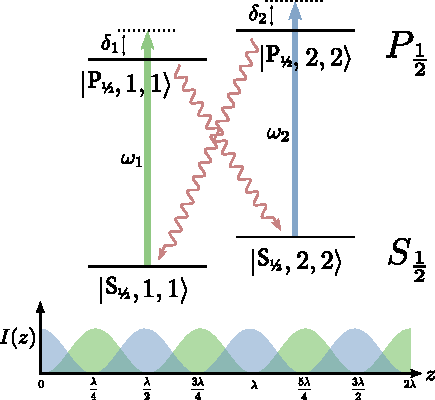
\includegraphics[width=0.65\textwidth]{figures/unsorted/cooling_simplified.pdf}
\caption{\label{fig:cooling_simplified}An idealised depiction of the cooling scheme, with repump lasers and undesired states not shown. Two lasers on the D$_1$ line are used for cooling, both linearly polarised, and arranged so as to form two interleaved standing waves. Both are blue detuned from the transitions they target, and they differ by about $6.8\,$GHz. This difference means that the alignment of the two standing waves can only be maintained over a distance of about a centimetre.}
\end{center}
\end{figure}

The scheme involves four lasers, two for cooling and two for repumping. For simplicity I will first focus on the cooling lasers only, depicted in Figure~\ref{fig:cooling_simplified}. Consider a rubidium atom at $z=0$ and in the $|1,1\rangle$ hyperfine groundstate. At this position the atom sees no light, as the intensity of the cooling laser labelled $\omega_1$ is zero, and it is in the wrong state to be pumped by the $\omega_2$ laser (which is not resonant with any transitions from the $|1,1\rangle$ groundstate).

As the atom moves rightward however, it will have to climb the repulsive potential hill formed by the $\omega_1$ laser. As it does so, its $|1,1\rangle$ excited state probability will increase, and along with it, the probability of spontaneous emission. Spontaneous emission will be most likely to occur near the top of the potential hill where the laser intensity---and hence the excited state probability---is greatest.

The most likely groundstate for the atoms to decay to from the $|1,1\rangle$ excited state is the $|2,2\rangle$ groundstate, and this is most likely to occur near $z=\frac\lambda4$. If this occurs, we now have an atom in the $|2,2\rangle$ groundstate at $z=\frac\lambda4$, a situation similar to that in which it started. Again, out atom now sees no light, but which laser has zero intensity and which targets the wrong transition are swapped.

As our atom continues rightward, it now has to contend with the potential hill formed by the $\omega_2$ laser, and is most likely to undergo spontaneous emission from the $|2,2\rangle$ excited state near the top of the potential hill. This time emission is most likely to put the atom into the $|1,1\rangle$ groundstate.

This process repeats, with atoms repeatedly climbing potential hills and being cooled. They spend approximately half their time in the $|1,1\rangle$ groundstate, allowing us to take advantage of the strong interspecies repulsion that that state entails for our two atomic species.

Of course, as is always the case, things aren't that simple. Whilst the two spontaneous decays mentioned above are the most likely, they are by no means the only possibilities. Some spontaneous decays will put the atoms back into the groundstate from which they came, with no harm done except a little extra heating from the photon recoil. Other decays however will put our atom into states that are not involved in the cooling scheme, where they will remain with no further cooling unless we do something about it. For this we need repump lasers (Figure \ref{fig:cooling_full}).

There are three states that the atom might end up in as a result of decay from the two excited states involved in the cooling process, and two repump lasers are used to excite them to three $P_\frac32$ states. Two of these transitions are similar enough that they can be addressed with the same laser.

\begin{figure}
\begin{center}
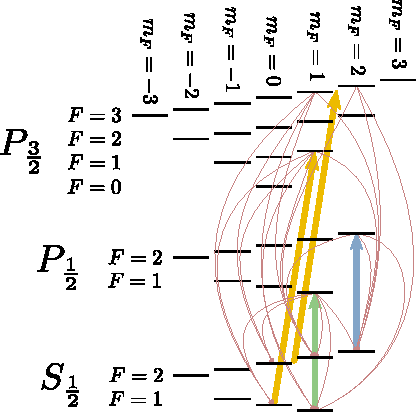
\includegraphics[width=0.65\textwidth]{figures/unsorted/cooling_full.pdf}
\caption{The full cooling scheme, including repump lasers (yellow), cooling lasers (blue and green), and all possible decay paths (red). The repump beam which is drawn in between two ground and excited states has a frequency equal to the average of those two transitions.}\label{fig:cooling_full}
\end{center}
\end{figure}

\subsection{Methods}

The cooling scheme was simulated for the case of a single atom, with the internal state of the atom modelled with the Schr\"odinger equation in the eigenbasis of the Hyperfine and Zeeman Hamiltonians (described in Section~\ref{sec:the_rubidium_D_line}), the state vector being a complex 32-vector\footnote{One complex number for each state in \figref{fig:cooling_full}.}. The dipole transition matrix elements coupling each pair of states were each computed as the appropriate linear sum of the dipole matrix elements at zero field, using the dipole approximation and the rotating wave approximation, as described in Section~\ref{sec:optical_dipole_transitions}. Since the corresponding Rabi frequencies depend on the laser intensity as well as the dipole matrix elements, they are functions of space, to be computed at each integration timestep as the atom moves through different intensities of the cooling beams. Following~\cite[p 4]{metcalf_laser_1999}, this produced a set of 32 coupled differential equations for the complex amplitudes of each state, of the form :

\begin{equation}
\ii\hbar\dv{t} c_e(t) = -\frac12e\sum_{g,\ n} E_n \langle g |  q_n | e \rangle c_g(t) \ee^{-\ii\delta_{nge}t},
\end{equation}
and
\begin{equation}
\ii\hbar\dv{t} c_g(t) = -\frac12e\sum_{e,\ n} E_n \langle g |  q_n | e \rangle c_e(t) \ee^{\ii\delta_{nge}t},
\end{equation}
where each $c(t)$ is the complex amplitude of one state; the $e$ indices are over the excited states and the $g$ indices over the groundstates; the $n$ indices are over the lasers, with $E_n$ being the amplitude of the $n$\textsuperscript{th} laser's electric field, $\delta_{nge}$ the detuning of the $n$\textsuperscript{th} laser from the transition between the $g$\textsuperscript{th} ground and $e$\textsuperscript{th} excited states, and $\langle g |  q_n | e \rangle$ the dipole moment between the $g$\textsuperscript{th} ground and $e$\textsuperscript{th} excited states for the polarisation of the $n$\textsuperscript{th} laser.

The external motion of the atom was modelled classically, with the atom having a definite position and velocity in one dimension. The force on the atom was computed from the dipole forces that the two groundstates involved in the cooling cycle experience due to the standing waves formed by the cooling beams. An expectation value of the dipole force was computed as:
\begin{align}
\ev{F} = \abs{\braket{1, 1}{\Psi}}^2F_{\ket{1, 1}} + \abs{\braket{2, 2}{\Psi}}^2F_{\ket{2, 2}},
\end{align}
where $F_{\ket{1, 1}}$ and $F_{\ket{2, 2}}$ are the dipole forces on the two groundstates, calculated using~\cite[eqn 3.16, p 33]{metcalf_laser_1999} with one standing wave offset from the other by a quarter wavelength. The forces on other groundstates are neglected since the repump beams do not have intensity gradients, and since the cooling beams are much further away from resonance for groundstates other than the two in the cooling cycle. Forces on excited states are also neglected---although the forces on the two excited states in the cooling cycle are not smaller than those on the corresponding groundstates, the excited state populations are small since the cooling beams are several linewidths away from resonance.

This expectation value of the dipole force was used to model the classical motion of the atom. Although the components of an atom in superposition would in reality spatially separate under the influence of a force that is different for different internal states of the atom, as in the Stern--Gerlach experiment, our atom only transitions between the two states subject to different forces via spontaneous emission, after which it is in an eigenstate. Accordingly, the expectation value calculation is always dominated by one of the two groundstates and the potential for Stern--Gerlach separation does not arise.

Spontaneous emission was simulated stochastically at each integration timestep, with probability of decay per unit time equal to the sum of populations in all excited states, multiplied by their decay rates (equal to the natural linewidths of each of the two fine-structure lines). Multiplying by the duration of one timestep, and comparing with a random number then determined whether a decay was to occur.

In the event of a decay, one excited state was randomly chosen with probability proportional to its population, and then one groundstate, weighted by the transition strengths from the excited state. All population was then put into that groundstate and the simulation continued, with one photon's worth of momentum in a random 1D direction added to the atom's momentum to account for photon recoil.

The equations of motion were solved using fourth order Runge--Kutta integration (Section~\ref{sec:rk4})

\subsection{Results}

\begin{table}
    \renewcommand{\arraystretch}{2.0}
    \makebox[\textwidth][c]{
    \begin{tabular}{|c|p{3.5cm}|r|r|c|}\hline
    Type & Transition(s) targeted & Detuning & Intensity (per beam) & Polarisation\\\hline
    cooling (standing wave) & $|S_\frac12,2,2\rangle\rightarrow |P_\frac12,2,2\rangle$ & + $66.6\,$MHz & $5.0\,$mW$\,$cm$^{-2}$ & $\pi$ \\
    cooling (standing wave) & $|S_\frac12,1,1\rangle\rightarrow |P_\frac12,1,1\rangle$ & + $31.9\,$MHz & $5.0\,$mW$\,$cm$^{-2}$ & $\pi$ \\
    repump (single beam) & \parbox{5cm}{\ \\ $|S_\frac12,2,1\rangle\rightarrow |P_\frac32,2,2\rangle$ \\
                           $|S_\frac12,2,0\rangle\rightarrow |P_\frac32,2,1\rangle$} & Midway between & $50.0\,$mW$\,$cm$^{-2}$ & $\sigma^+$ \\
    repump (single beam) & $|S_\frac12,1,0\rangle\rightarrow |P_\frac32,1,1\rangle$  & $0$ & $10.0\,$mW$\,$cm$^{-2}$ & $\sigma^+$ \\

    \hline
    \end{tabular}
    }
    \caption{The parameters used in the laser cooling simulations. There are four lasers, each with a specified polarisation, intensity, and detuning from the transition it targets.}\label{table:numbers}
\end{table}

The laser parameters used in the simulation are shown in Table~\ref{table:numbers}. The magnetic field strength used was $34\unit{G}$. The detunings of the cooling beams were chosen based on an approximate calculation in order to produce a scattering rate of $2\times10^{5}$ photons per second in the simulation.

The simulation was run for $715$ million integration timesteps of size $\upDelta t=20\unit{ps}$,\footnote{Corresponding to approximately ten timesteps per oscillation of the fastest oscillating terms, which oscillate at a rate close to half the $6.8\unit{GHz}$s hyperfine splitting of the rubidium groundstates.} for a total of 14.3 milliseconds of simulation time. This took $14$ days of computer time. In that time, the atom moved a maximum distance of $26\unit{\upmu m}$ from its starting position, and its final position was $790\unit{nm}$ from its starting position. The atom's initial velocity was $195 \unit{mm\,s}^{-1}$, and during the simulation it reversed the direction of its velocity $2226$ times. $4103$ photons were emitted, for an average scattering rate of $2.87\times10^\up{5}$ photons per second---slightly higher than the target rate.

Computing the time-averaged kinetic energy of the atom over the whole simulation as:
\begin{equation}
\ev{E_\up{K}} = \frac12 m_\up{Rb} \langle v^2 \rangle,
\end{equation}
and assuming the single atom ergotically sampled a sufficient fraction of the possible state space, we can compute the 1D temperature that a cloud of atoms subject to this cooling would have after being allowed to come to equilibrium using
\begin{align}
\frac12 k_\up{B} T_\up{1D} = \ev{E_\up{K}},
\end{align}
which gives  $T_\up{1D} = 16.2\unit{\upmu K}$, well below the Doppler temperature $T_\up{D} = 146\unit{\upmu K}$~\cite{steck_rubidium_2015}. A histogram showing the time the atoms spent at different velocities is show in Figure~\ref{fig:cold_atom}. This one-dimensional temperature corresponds to $\approx30E_\up{r}$ where $E_\up{r}$ is the rubidium recoil energy. Given that the potassium vortex potentials are at about $15E_\up{r}$ deep without a Feshbach resonance at a density of $1\times10^{15}\unit{cm}^{-3}$ and only $\approx 2.0E_\up{r}$ at the more realistic density of $1\times10^{14}\unit{cm}^{-3}$, and that the atom only spends about half its time in the state subject to the Feshbach resonance, this cooling would only be sufficient to keep rubidium atoms trapped in vortex cores if the Feshbach resonance enhances the interspecies scattering length by a factor of $\approx 2$ for a $1\times10^{15}\unit{cm}^{-3}$ condensate or a factor of $\approx 30$ for a $1\times10^{14}\unit{cm}^{-3}$ condensate. While a factor of $2$ is easily achievable, a factor of $30$ is not, indicating that the minimum density compatible with tracer particles at this temperature being trapped is between $1\times10^{14}\unit{cm}^{-3}$ and $1\times10^{15}\unit{cm}^{-3}$.

\begin{figure}
\begin{center}
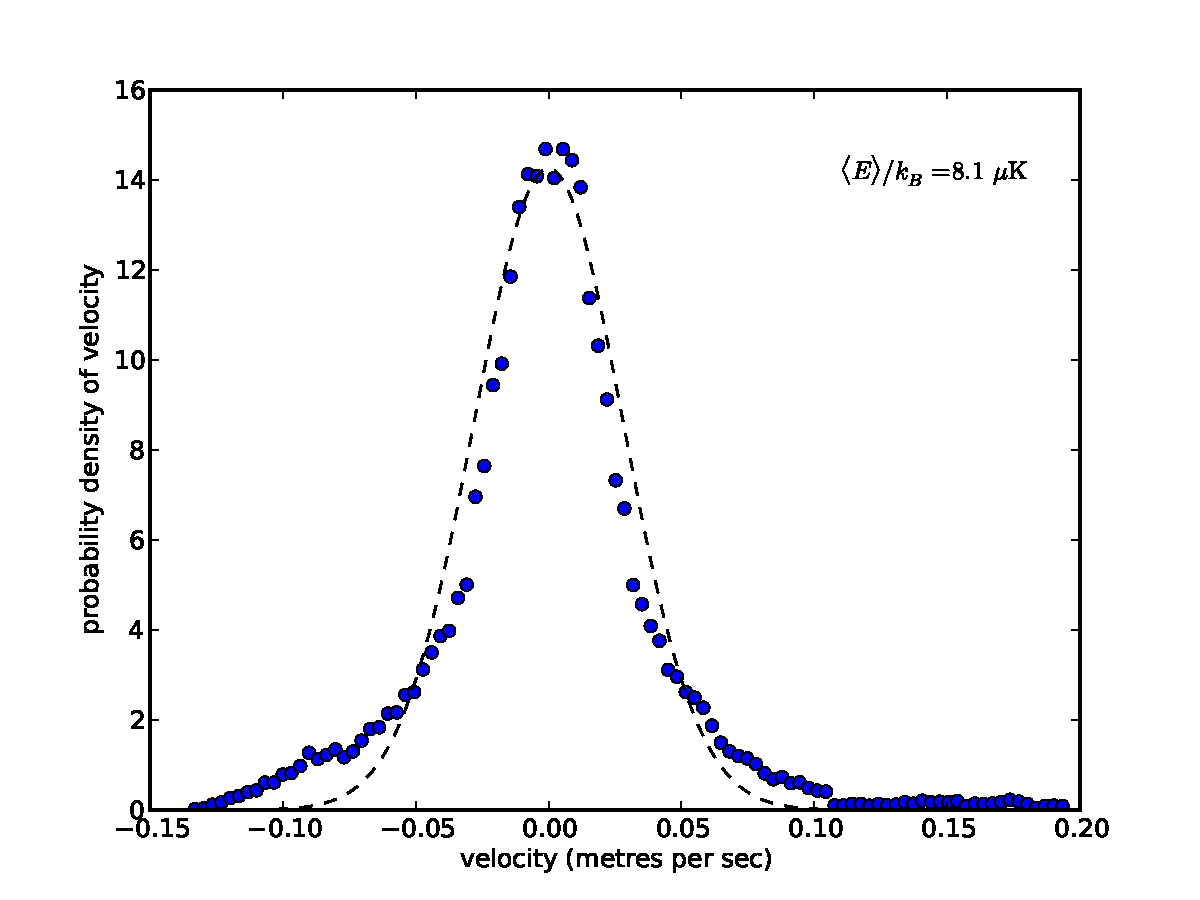
\includegraphics[width=\textwidth]{figures/unsorted/cold_atom.pdf}
\caption{\label{fig:cold_atom} Histogram of atom velocity over time, normalised as a probability density. A best-fit Maxwell--Boltzmann distribution is shown as the dotted line. It is no surprise that it is not a good fit---there is no thermalisation happening since there is only one atom and no collisions. The average energy is more informative than the fit parameters for determining the temperature that an ensemble of such atoms would have if they were allowed to thermalise. The long tail visible to the right is the atom's initial slowdown from its starting velocity.}
\end{center}
\end{figure}

This simulation has not, however, been optimised---the results presented here represent the only extended simulation of the scheme, and no attempt has been made to scan over parameter space to see if the temperature can be made lower. As mentioned the simulation was computationally expensive, and so optimisation would be impractical if performed using the same code. However, a significant speed up would be possible by correcting some inefficiencies. Firstly, one could exclude from the simulation the atomic states that were shown in the first run never to become occupied---the the states with no arrows leading to them in \figref{fig:cooling_full}. This will eliminate approximately two thirds of the states, and since the simulation is quadratic in the number of states, this should provide an approximately $10\times$ increase in simulation speed. More importantly, lasers that are detuned with respect to a given transition by approximately the hyperfine splitting of $6.8\unit{GHz}$ should be discarded in the coupling term for that transition. The inclusion of these fast rotating terms---which are so far detuned as to cause negligible population transfer---was the limiting factor in the simulation timestep size, which would otherwise be determined by the next fastest rotating terms on the order of tens of $\unit{MHz}$ instead of $\unit{GHz}$. This would lead to a likely dramatic speedup as well, making repeated runs of the simulation feasible.

\subsection{Vortex-assisted Sisyphus cooling}\label{sec:vortexcooling}

Another idea for a cooling scheme is to use the vortex potential itself as a spatial discriminator for transferring atoms between states. Similar to how a \mot\ traps atoms by bringing them into resonance with optical pumping only when they are some distance from the trap's centre, one might use the shape of the vortex potential to bring an \rf\ or microwave transition into resonance only when trapped tracer particles are some distance away from the centre of a vortex core. This method was proposed by Prof.~Helmerson whilst considering different possibilities for cooling atoms in vortex cores, and I considered which states might be appropriate to implement the scheme in. I have not simulated this scheme, but present it here because the reason it is difficult to simulate is an example of the difficulty that led me to develop the hidden variable semiclassical method presented in Chapter~\ref{chap:hvsc}.

\begin{figure}
\begin{center}
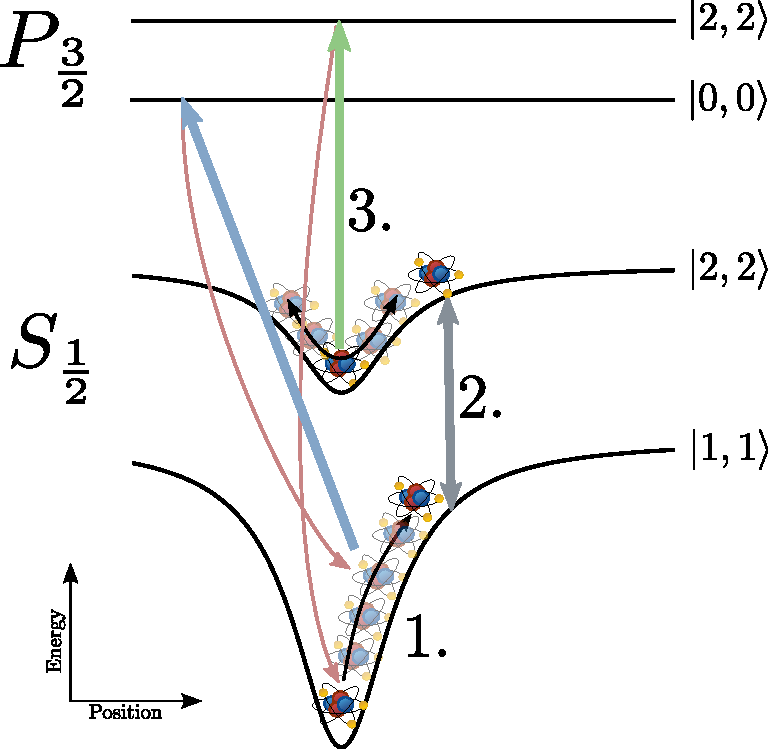
\includegraphics[width=0.7\textwidth]{figures/unsorted/vortexcooling.pdf}
\caption{A basic description of the vortex-assisted cooling scheme.
\protect\\
1. The rubidium atom in its $|1,1\rangle$ groundstate repeatedly scatters photons from the laser marked with the blue arrow, climbing the vortex potential as it does so. The optical transition's linewidth is large enough that the energy shift due to the vortex potential does not move it off resonance.
\protect\\
 2. An \rf\ or microwave transition however, has an extremely narrow linewidth; its effective linewidth is dependent only on the \rf/microwave power. A microwave transition (grey arrow) comes into resonance only when the atom moves sufficiently far from the vortex core's centre, and coherently transfers population into the $|2,2\rangle$ groundstate.
 \protect\\
 3. The atom oscillates back and forth in the much shallower vortex potential that its $|2,2\rangle$ groundstate experiences. It is pumped weakly by the laser marked with the green arrow, and after a random time delay (and hence at a random position) spontaneously decays back to the $|1,1\rangle$ groundstate.
}\label{fig:vortexcooling}
\end{center}
\end{figure}

The basic idea of the vortex-assisted cooling scheme is outlined in Figure~\ref{fig:vortexcooling}. In the presence of the Feshbach resonance, atoms in the $\ket{1,1}$ state scatter some tens of photons, using whichever transition is most likely to have them decay to the same groundstate with minimal repumping (the $\ket{0,0}$ excited state on the $D_2$ line looks to be the best choice). As the atom scatters photons, it climbs the side of the vortex potential, converting the kinetic energy obtained from photon recoil into potential energy.

Due to the state-dependence of the interspecies scattering length, the vortex potentials for different states have different depths, especially when one is enhanced by a Feshbach resonance. This means that the \rf\ or microwave frequency required to transition between the different hyperfine states and Zeeman sublevels varies as a function of space, and can be tuned so as to only be resonant with atoms which have nearly escaped the vortex core.

When the atom enters the region resonant with said \rf\ or microwave radiation, it is then transferred into a different hyperfine or Zeeman state, for example the $\ket{2,2}$ groundstate, and the hope is that it then lacks the kinetic energy to escape the (shallower) vortex potential it then finds itself in. Rather, it oscillates back and forth in the well until a weak laser pumps it back into the $\ket{1,1}$ groundstate via spontaneous emission from some excited state (again chosen to maximise the decay probability to $\ket{1,1}$; the $\ket{2,2}$ $P_\frac32$ excited state looks to be a good choice.)

After completing this cycle, statistically the atom will be closer to the centre of the  $\ket{1,1}$ vortex potential than when it left the $\ket{1,1}$ state. Provided its corresponding drop in potential energy makes up for the photon scattering (which provides fluorescence imaging), then it comprises a cooling and imaging scheme capable of keeping the atoms trapped in the vortex cores. It is yet another Sisyphus effect, with the atom climbing steep vortex potential hills and descending shallower ones.

However, this scheme cannot be simulated in the same manner as the laser cooling scheme presented in Section~\ref{sec:laser_cooling_simulations}. The reason is that the \rf\ or microwave transition depicted as the grey arrow in~\figref{fig:vortexcooling} is coherent, and as such leads to state vectors that are superpositions of the two hyperfine or Zeeman sublevels, with no one state dominating the superposition. Since (crucially for the cooling scheme), the two states are subject to different potentials, an atom in such a superposition would undergo Stern--Gerlach separation. Unlike the laser cooling scheme from the previous section, since no one state dominates the superposition at a given time, the expectation value of the two forces does not accurately describe the motion of the atom. To accurately simulate this cooling scheme, a semiclassical method able to reproduce this Stern--Gerlach separation would likely be necessary. This realisation, along with similar difficulties in simulations of Majorana losses in evaporative cooling during collaboration with Drs.~Turner and Anderson and Chris Watkins led me to develop the hidden-variable semiclassical method, discussed in Chapter~\ref{chap:hvsc}.

% Paths: bilbo.tk: ~/laptop_backup/Desktop/current_work/sympathetic_cooling/
%                  ~/oldserver/bilbo/particle_tracking_higher_scattering_length
%                  ~/laptop_backup/Desktop/current_work/paper%20simulations/
%                  ~/laptop_backup/Desktop/current_work/paper
%                  ~/laptop_backup/Desktop/current_work/DPGPoster
% Compare to honours thesis - don't include stuff already in honours thesis!

\section{Discussion and conclusion}

Sisyphus cooling: maybe. Looks ok but I have disregarded heating of the condensate. Short imaging at high intensity could be used to view vortices but maybe not continuously unless more cooling is added. Imaging assumes we remain in the 1,1 state, so would require repumping. Strong feshbach resonances induce inelastic collisions, so that is a limitation
% (https://journals.aps.org/prl/abstract/10.1103/PhysRevLett.82.2422).

In 3D the cloud of atoms surrounding would obscure things a bit more since they would be in front of the BEC as well.

laser cooling: also maybe - can be optimised, but in 3D might be different, is impractical given the number of lasers and the funky alignment, which can only be maintained over a distance of [something].

This chapter doesn't establish definitively whether the scheme will work in practice but provides enough of a wink in its direction to suggest an experimental attempt.


\setcounter{chapter}{5}

\chapter{Hidden variables for semiclassical models with state-dependent forces}

Hidden-variable theories~\cite{GENOVESE2005319, PhysRevA.71.032325} are interpretations of quantum mechanics that posit definite states underlying quantum state vectors, such that quantum indeterminacy is an illusion---an emergent phenomenon rather than a fundamental fact. Bell's theorem~\cite{Bell:111654} proves that any such theory must be \emph{nonlocal} in order to explain all the predictions of quantum mechanics, and perhaps in light of this, most physicists surveyed~\cite{schlosshauer_snapshot_2013} do not believe that hidden variables underlie physical reality.

However, by framing quantum systems in classical terms, hidden-variable theories can provide an excellent computational tool for \emph{approximate} models of quantum systems, when it is reasonable to approximate some degrees of freedom as classical, yet other degrees of freedom need to be modelled quantum mechanically. Just as hidden-variable theories have framed the quantum world in terms that are agreeable to the classical view of the world in the minds of some interpreters of quantum mechanics, so can they bridge the gap between a \emph{simulated} quantum world and a \emph{simulated} classical world coexisting in the same computer simulation.

In this chapter I describe what I call the `hidden-variable semiclassical' (\textsc{hvsc}) method: a method of combining quantum simulations with classical simulations, with hidden variables bridging the gap between the classical and quantum degrees of freedom. In this introduction I describe existing semiclassical methods, the manner in which their quantum and classical parts are typically coupled based on expectation values (which I'm calling the `Ehrenfest method'), and in which regimes this can be inaccurate---namely the Stern--Gerlach experiment and similar situations in which considerable entanglement between motional and internal degrees of freedom of atoms can develop.

In Section~\ref{sec:semiclassical_methods} I give an overview of what a semiclassical method is, their most common implementation and in what situations this is insufficiently accurate, motivating the need for an improved method. In Section~\ref{sec:hidden_variable_theories} I give the technical definition of a hidden-variable theory, and motivate the use of such a theory for coupling quantum and classical degrees of freedom in such a way that the a semiclassical model can be made to agree more closely than the Ehrenfest method with the underlying fully quantum model it is approximating, and ultimately, with experiment. In Section~\ref{sec:overview_of_method} I then go into the implications of welcoming a hidden variable into a semiclassical model, including additional required assumptions and approximations, and in Sections~\ref{sec:implementation_details} and~\ref{sec:decoherence} I go into detail deriving the equations of motion for the model and presenting some algorithmic and computational details. Finally in Section~\ref{sec:HVSC_algorithm}, having provided all the background arguments and details, I present the complete algorithm(s), before showing simulation results in Section~\ref{sec:HVSC_results} that compare the model to the underlying exact Schr\"odinger wave equation, and concluding in Section~\ref{sec:HVSC_discussion} with further discussion of the method's benefits and limitations.

During writing this thesis, I discovered that the ideas underpinning this method are (perhaps unfortunately) not original, and that the `surface hopping' method enjoys widespread use and continued development in the field of computational chemical physics~\cite{doi:10.1063/1.459170, A801824C, doi:10.1146/annurev-physchem-040215-112245, doi:10.1063/1.1675788, doi:10.1063/1.3575588, doi:10.1063/1.447708, doi:10.1063/1.3489004, doi:10.1063/1.2715585, C6SC01319H, doi:10.1063/1.479058, doi:10.1063/1.4829856}. A preprint of an early version of my method~\cite{billington_monte_2015} bears a striking resemblance to a paper by Tully~\cite{doi:10.1063/1.459170}, the pioneer of surface hopping methods. Use of these ideas do not however appear to be common in cold atom physics, but with direct simulation of evaporative cooling and laser cooling schemes becoming increasingly plausible given the increasing availability of computational power as well as efficient molecular dynamics techniques such as Direct Simulation Monte Carlo (\textsc{dsmc})~\cite{DIETRICH1996328}, this sort of convergent evolution of numerical techniques is perhaps not surprising. Throughout this chapter I make comparisons between my own methods and those in the existing surface hopping literature. Some long-standing limitations of my method may be resolved in light of what I have now read in the surface hopping literature, leading to speculative improvements that I have yet to test. These improvements are outlined in this chapter, and flagged as speculative.

\section{Semiclassical models}\label{sec:semiclassical_methods}

A semiclassical model is any model in which some degrees of freedom are treated quantum mechanically, and others classically. The most common combination is that of treating an atom's internal electronic state quantum mechanically and its motional degree of freedom classically. This is useful whenever the quantum effects of the atom's motion are not of interest, for example if temperatures are high and thus atomic wavelengths are short---such that quantum effects simply aren't visible in the motion of the particles and so they can accurately be modelled as classical billiard balls. The energy gaps between different electronic states of atoms are so large however that only at very high temperatures (at which atoms ionise anyway) do they start to appear as a continuum compared to thermal energy scales, and the interaction of different spin states of the atom with different optical and magnetic fields does not make them appear as classical continua either. Thus, quantum effects can be ignored for the centre of mass motion of the (relatively heavy) atom, but not for the relative motion of its (much lighter) electrons with respect to the nucleus, or for the nuclear and electronic spin degrees of freedom~\cite{doi:10.1063/1.459170}.

In this regime, atoms are often modelled semiclassically, with these internal degrees of freedom modelled using a state vector $\ket\chi$ evolving according to a Hamiltonian $\hat H$ via the Schr\"odinger equation, and the centre of mass motion modelled as a position $\vec r$ and velocity $\vec v$ evolving according to Newton's second law (\figref{fig:semiclassical}).

\begin{figure}[t]
    \centerfloat
    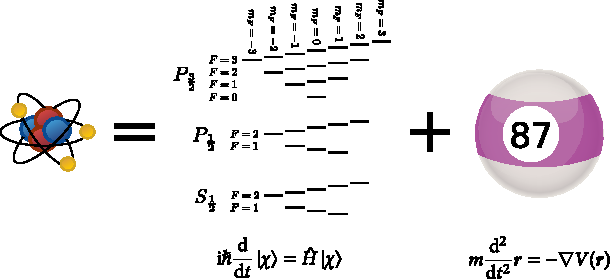
\includegraphics[width=0.75\textwidth]{figures/hidden_variables/semiclassical.pdf}
    \caption{Artist's depiction of a semiclassical atom.}
    \label{fig:semiclassical}
\end{figure}

Once one has defined a potential function $V(\vec r)$ and a Hamiltonian (also possibly varying with space) $\hat H(\vec r)$, and other possible additions,\footnote{Such as using a Monte-Carlo wavefunction method~\cite{Molmer:93, RevModPhys.70.101} to model the effect of spontaneous emission on $\ket\chi$, and modifying $\vec v$ instantaneously by a random-direction recoil velocity upon each photon emission.} ones job is done and the rest can be left to numerical differential equation solvers to evolve some concrete vector representation $\vec\chi$ of $\ket\chi$ as well as the state variables $\vec r$ and $\vec v$ for motional degree of freedom in time according to the coupled differential equations
\begin{align}\label{eq:simple_semiclassical_first}
\dv{t}\ket\chi &= -\frac\ii\hbar \hat H(\vec r)\ket\chi,\\
\dv{t}\vec v &= -\frac1m\nabla V(\vec r),\\
\dv{t}\vec r &= \vec v\label{eq:simple_semiclassical_last}.
\end{align}
In the next subsection I explain why it's not always that simple.

\subsection{Stern--Gerlach separation and evaporative cooling}

In the Stern--Gerlach experiment~\cite{gerlach_experimentelle_1922}, particles with quantum spin and a magnetic moment---atoms for example---are fired as a beam through a region of space with a magnetic field gradient. The well known result is that two clusters (if the atoms are spin-$\frac12$) of positions are observed once the beam emerges, rather than a continuous smear of positions, indicating that angular momentum---like many quantities in quantum mechanics---is quantised.

This is the case even if one spin-polarises the particles before they are passed through the magnetic field gradient, say putting them in an eigenstate of the $\hat F_x$ operator. Then, if the magnetic field is along the $z$ direction, and the gradient is also in the $z$ direction, two clusters of positions are also observed, even though all particles were in the same state when they entered the region in which there was a magnetic field gradient. This is a display of the indeterminacy of quantum mechanics: even though all particles had the same initial state, there were nonetheless different outcomes for each particle.

The outcome of the Stern--Gerlach experiment is a consequence of quantum mechanics, to be sure, but it has little to do with the wave nature of the atoms themselves. If we introduced some double slits for the atoms to pass through in addition to the magnetic field gradient, then we would be seeing the wave nature of the atoms as interference patterns at the detection screen at the end of the experiment. But if we do not, and if the particles have short de-Broglie wavelengths, then quantum mechanics is not apparent in the motion of the particles through space---except via the influence of spin on seemingly choosing one trajectory or the other. The effect is well understood quantum mechanically, but is difficult to model semiclassically because even if we are happy to approximate wavepackets as small, the wavepackets do not take a single trajectory. Rather they split into two wavepackets, with the part of the superposition corresponding to one spin projection state (along the direction of the local magnetic field) moving one way, and the part of the superposition with the other spin projection going the other way. The trajectories can still be quite classical, it's just that there are two of them.

A similar situation exists in \textsc{rf} evaporative cooling (Section~\ref{sec:evaporative_cooling}) of cold atoms en-route to \textsc{bec}. Atoms are confined in a magnetic trap, and are spin polarised so as to be fully spin-down (for $^{87}$Rb this is the trapped state) with respect to the local magnetic field at the position of each atom. The magnetic field's direction---not just  its magnitude---varies in space, and so different atoms have different spins, but they are all spin-down with respect to the quantisation axis of the local magnetic field. As the atoms move through space, they move in orbits---punctuated by collisions---about the magnetic field zero at the centre of the trap, since they feel a force $F\propto-\nabla\abs{\vec B}$ due to the gradient of the Zeeman potential. Provided they are moving slowly (specifically, provided their Larmor precession period is short compared to the time the magnetic field as seen by the atom takes to change by a non-negligible fraction of its current value), the atoms' spins adiabatically follow the local field and remain spin-down, even as the field as seen by each atom fully reverses its direction every half orbital period.

Near the centre of the trap where the atoms are moving faster, the fields are small and therefore have large fractional derivatives and lead to large Larmor periods, adiabaticity no longer holds and the atoms may make spin transitions with respect to their local magnetic field. Once an atom passing close to the field zero has evolved into a superposition of spin projection states with respect to the local field, it is in a situation identical to the initial condition of the Stern--Gerlach experiment, causing the spin projection components to spatially separate in the magnetic field gradient. The spin-up component is anti-trapped and repelled from the centre of the trap, and the zero spin projection component (since the groundstate of $^{87}$Rb is spin-$1$) feels no force and moves in a straight line. The spin-down component continues on an orbit about the field zero which is just as tight as before, unaffected by the close approach to the field zero other than being reduced in amplitude. Eventually a collision occurs, either with other atoms or with the walls of the vacuum system and the wavefunction collapses to choose one of these options, leading to atoms probabilistically leaving the trap (called Majorana losses~\cite{Majorana1932, PhysRevLett.74.3352}) or remaining trapped. Again, the trajectories can still be quite classical, it's just that there are three of them, and which is taken is probabilistic.

How can we model these effects semiclassically? Equations~\eqref{eq:simple_semiclassical_first} to~\eqref{eq:simple_semiclassical_last} are not sufficient, because exists no single classical potential $V(\vec r)$ that can describe the motion of the atoms. Rather, the atoms feel a different force depending on which spin state they are in. Just as the Hamiltonian can be a function of space, so can the potential be a function of the internal state of the atom: $V = V(\vec{r}, \ket\chi)$. Ehrenfest's theorem~\cite{Ehrenfest1927} states that
\begin{align}
m\dv[2]{t}\ev{\hat{\vec r}} = - \ev{\nabla \hat V},
\end{align}
where the expectation values are over all degrees of freedom, not just motional. If we approximate a small wavepacket centred at the position $\vec r$ in order to ignore the wave nature of the atoms, this becomes:
\begin{align}
m\dv[2]{t} \vec r = - \nabla \matrixel{\chi}{\hat V(\vec r)}{\chi},
\end{align}
where the operator $\hat V(\vec r)$ now only acts on the subspace of the internal state of the atom, since we have already taken an expectation value over (a small region of) space. Provided all potentials the atom is subjected to are included in the Hamiltonian for its internal state (including any energy offsets that do not
depend explicitly on the internal state), this is nothing but
\begin{align}
m\dv[2]{t} \vec r = - \nabla \matrixel{\chi}{\hat H(\vec r)}{\chi},
\end{align}
where $\hat H$ is the Hamiltonian describing the evolution of the atom's internal state. We now can construct the \emph{Enhrenfest semiclassical method} describing how the \emph{expectation value} of a well localised atom's position evolves with time:

\begin{align}\label{eq:ehrenfest_semiclassical_first}
\dv{t}\ket\chi &= -\frac\ii\hbar \hat H(\vec r)\ket\chi,\\
\dv{t}\vec v &= -\frac1m\matrixel{\chi}{\hat H(\vec r)}{\chi},\\
\dv{t}\vec r &= \vec v\label{eq:ehrenfest_semiclassical_last}.
\end{align}

The Ehrenfest semiclassical method is the same as the simple semiclassical method~\eqref{eq:simple_semiclassical_first} to~\eqref{eq:simple_semiclassical_last}, except that it has an answer to the question ``What should we use for $V(\vec r)$ when the atom is in a superposition of states that feel different potentials?'', which is ``use the expectation value''. 

This is all well and good if the expectation value of position is a good approximation to the situation being modelled. But in the Stern--Gerlach experiment or a Majorana spin flip in a magnetic trap, the expectation value of position is a poor match to reality. In the Stern--Gerlach experiment beginning with spin-polarised atoms, a trajectory subject to the mean force or potential (which are both zero for a $50:50$ superposition) would land in a single blob in the middle of the screen, rather than two blobs displaced from the centre. In the case of an atom approaching the field zero in a magnetic trap, use of the mean force would result in the atom broadening its orbit somewhat, rather than splitting into multiple possible trajectories (Figure~\ref{fig:evap_problem}). Semiclassical simulations of evaporative cooling performed by Christopher Watkins (unpublished) displayed an unphysical heating of the atom cloud that I believe is due to the Ehrenfest method's inability to model Stern--Gerlach separation. In a real magnetic trap during evaporative cooling to Bose--Einstein condensation, the mean free path is large enough that the part of the wavepackets that are no longer trapped will usually leave the trap without colliding with any other atoms. This means that the energy the untrapped and anti-trapped components have gained (relative to the trapped component) moving away from the field zero is not usually shared with other atoms upon collision---the extra energy leaves with the atoms. However, if a close approach to the magnetic field zero merely means a broadening of the atoms orbit, then the extra energy does not leave as fast, if at all, and can be shared with other atoms via collisions, turning what would have been an atom loss effect into an overall gradual heating of the cloud. 

\begin{figure}[t]
    \centerfloat
    \includegraphics[width=0.75\textwidth]{figures/hidden_variables/evap_problem.pdf}
    \caption{When atoms pass near to the field zero in a magnetic trap, their wavepackets diverge in space as multiple trajectories, each corresponding to one local spin projection state. For example, if a spin-$\frac12$ atom undergoes a partial spin-flip such that it has a ten percent probability of being spin-up, the end result will be two approximate trajectories. One trajectory describes the motion of a wavepacket that is fully spin-up, and one fully spin-down, with the spin-down wavepacket's squared amplitude equal to $0.1$. The Ehrenfest semiclassical method however can only model a single trajectory, and the end result when using this method is a single trajectory being approximately the mean of the two actual trajectories, and retaining a $90:10$ ratio of spin-down:spin-up state populations.}
    \label{fig:evap_problem}
\end{figure}

So how can we modify a semiclassical method to choose only one trajectory? Firstly, since each trajectory corresponds to one of the internal states (though some might be degenerate), our model must choose an internal state and use the classical trajectory corresponding to that internal state only. Secondly, since all atoms begin in identical states and yet some take one trajectory and some another, this choice must be probabilistic. Finally, the probabilities must be consistent with those from quantum mechanics, i.e. the Born rule: the probability of an atom taking each trajectory must be proportional to the squared amplitude of the internal state of the atom, projected onto the eigenstate corresponding to that trajectory.

There exists a category of theories dealing with precisely this question of how to choose a specific state of a quantum system in a stochastic way, such that the probability of having chosen a state is equal to that given by quantum mechanics. Such theories are called \emph{hidden-variable} theories, and any parameter, variable or label specifying which state has been chosen is a \emph{hidden variable}.

\section{Hidden-variable theories}\label{sec:hidden_variable_theories}

In his paper \emph{Quantum computing and dynamical quantum mdels}, Aaronson defines a \emph{dynamical quantum model}~\cite{aaronson_quantum_2002}:

\begin{quote}
A \emph{dynamical quantum model} assigns an eigenstate to a specified observable even when no measurement is made, and gives a stochastic evolution rule for that eigenstate. Such a model yields a distribution of classical histories of a quantum state.
\end{quote}
In a later paper, \emph{Quantum computing and hidden variables}, superseding the first, Aaronson renames dynamical quantum models to \emph{hidden-variable theories} and instead defines~\cite{PhysRevA.71.032325}:
\begin{quote}
For us, a hidden-variable theory is simply a way to convert a unitary matrix that maps one quantum state to another, into a stochastic matrix that maps the initial probability distribution to the final one in some fixed basis.
\end{quote}
This is what a hidden-variable theory is for the purposes of this chapter as well. Though the first paper is superseded by the second, the definition it gives is more tangible for us---we wish to \emph{assign an eigenstate} to our atoms (choose one of the internal states in order to decide which trajectory to follow), and have a \emph{stochastic evolution rule} for which eigenstate is chosen at any one time (allow the atom to begin taking a different trajectory if it makes transitions between states), probabilistically depending on the change in quantum populations of the states.

But the second definition is more specific. The stochastic evolution rule is in the form of a stochastic matrix, with elements equal to transition probabilities for some time interval. And the rule should be in some way based on the unitary evolution that the quantum system evolves according to in the same interval of time, such that the initial and final probabilities of the stochastic matrix and unitary evolution agree. That is, if a quantum state $\ket\chi$ evolves in a certain basis $\{\ket{\chi_i}\}$according to a unitary $\hat U(t^\prime, t)$:
\begin{align}
\left[\begin{matrix}
c_1(t^\prime)\\c_2(t^\prime)\\c_3(t^\prime)\\\vdots
\end{matrix}\right]
= \left[\begin{matrix}
U_{11}(t^\prime, t) & U_{12}(t^\prime, t) & U_{13}(t^\prime, t)&\hdots\\
U_{21}(t^\prime, t) & U_{22}(t^\prime, t) & U_{23}(t^\prime, t)&\hdots\\
U_{31}(t^\prime, t) & U_{32}(t^\prime, t) & U_{33}(t^\prime, t)&\hdots\\
\vdots & \vdots & \vdots & \ddots
\end{matrix}\right]
\left[\begin{matrix}
c_1(t)\\c_2(t)\\c_3(t)\\\vdots
\end{matrix}\right],
\end{align}
where $c_i = \braket{\chi_i}{\chi}$ and $U_{ij}(t^\prime, t) = \matrixel{\chi_i}{\hat U(t^\prime, t)}{\chi_j}$, then a hidden-variable theory is a matrix-valued function $S(U(t^\prime, t), \vec\chi(t)))$, where $\vec\chi(t)$ and $U(t^\prime, t)$ are the vector and matrix representations of the state vector $\ket{\chi(t)}$ and unitary $\hat U(t^\prime, t)$ in the $\{\ket{\chi_i}\}$ basis, that satisfies
\begin{align}
\left[\begin{matrix}
\abs{c_1(t^\prime)}^2\\\abs{c_2(t^\prime)}^2\\\abs{c_3(t^\prime)}^2\\\vdots
\end{matrix}\right]
= \left[\begin{matrix}
S_{11}(t^\prime, t) & S_{12}(t^\prime, t) & S_{13}(t^\prime, t)&\hdots\\
S_{21}(t^\prime, t) & S_{22}(t^\prime, t) & S_{23}(t^\prime, t)&\hdots\\
S_{31}(t^\prime, t) & S_{32}(t^\prime, t) & S_{33}(t^\prime, t)&\hdots\\
\vdots & \vdots & \vdots & \ddots
\end{matrix}\right]
\left[\begin{matrix}
\abs{c_1(t)}^2\\\abs{c_2(t)}^2\\\abs{c_2(t)}^2\\\vdots
\end{matrix}\right].
\end{align}
In essence, if quantum unitary evolution takes amplitudes to amplitudes, a hidden-variable theory takes probabilities to probabilities. Thus the elements of $S$ are conditional probabilities---or transition probabilities---for a hidden variable $\eta(t)$, giving the chance that the state $\ket{\chi_\eta} \in \{\ket{\chi_i}\}$ assigned by the hidden variable will change from one to another in the given time interval:
\begin{align}\label{eq:conditional_probability}
\Pr(\eta(t^\prime){=}i|\eta(t){=}j) = S_{ij}(U(t^\prime, t), \vec\chi(t)).
\end{align}
There are many ways to define functions $S$ that satisfy this condition. The simplest is to ignore the unitary completely and set $S_{ij} = \abs{c_i(t^\prime)}^2$, which yields:
\begin{align}
\Pr(\eta(t^\prime){=}i|\eta(t){=}j) = \abs{c_{i}(t^\prime)}^2,
\end{align}
that is that the hidden variable $\eta$ is equally likely to transition to a given value regardless of its previous value, and regardless of the unitary, and that that the conditional transition probability from all input states is just the squared amplitude of the final state. This theory represents a hidden variable that jumps between states randomly based on their population, with no regard for its history or whether there were actually amplitude flows between the states between which it is transitioning. Nonetheless, this theory, called \emph{product theory}~\cite{PhysRevA.71.032325}, matches the definition of a hidden-variable theory---$S$ is a stochastic matrix, and the hidden variable on average will spend an amount of time in each state consistent with the Born rule.

Aaronson outlines some additional axioms~\cite{PhysRevA.71.032325} that hidden variables ought to satisfy, if we are to take them seriously, including reasonable statements about symmetries, and insensitivity to small perturbations. He goes on to prove that the properties cannot all be satisfied simultaneously, but some theories satisfy more of them than others.

It is convenient to introduce the matrix $P$ of absolute transition probabilities. Summing~\eqref{eq:conditional_probability} over all possible initial values of the hidden variable yields the absolute probability of it having a particular final value after the given time interval:
\begin{align}
\Pr(\eta(t^\prime){=}i) 
= \sum_j \Pr(\eta(t^\prime){=}i|\eta(t){=}j) \Pr(\eta(t){=}j),
\end{align}
which, recognising that the final and initial probabilities must be the final and initial squared amplitudes of the state vector, can be rewritten:
\begin{align}
\abs{c_i(t^\prime)}^2
= \sum_j S_{ij}(U(t^\prime, t), \vec\chi(t)) \abs{c_j(t)}^2.
\end{align}
We now define the matrix of absolute transition probabilities $P$:
\begin{align}\label{eq:P_matrix_def}
P_{ij} = S_{ij}(U(t^\prime, t), \vec\chi(t)) \abs{c_j(t)}^2,
\end{align}
such that:
\begin{align}
\abs{c_i(t^\prime)}^2
= \sum_j P_{ij}.
\end{align}
So we have that $P$ has row sums equal to the final squared amplitudes.
And, because $P_{ij} = S_{ij}\abs{c_j(t)}^2$ and $S$ is a stochastic matrix with column sums equal to one,\footnote{In order to more clearly compare to quantum evolution, we are using \emph{left stochastic} matrices, which multiply column vectors of probabilities from the left, contrary to the most common convention for stochastic matrices which is to multiply row matrices from the right. Thus $S$ has unit column sums, whereas the corresponding right stochastic matrix (its transpose) would have unit row sums.} we have that $P$ must have row sums equal to the initial squared amplitudes.

Now that we have introduced $P$ and shown what its row and column sums must be, we come to a particularly simply defined hidden-variable theory called the Schr\"odinger theory, discussed in Aaronson's hidden variables paper~\cite{PhysRevA.71.032325}. The idea is to form $P$ by starting with the matrix of absolute values of $U$, and simply scaling its rows and columns to have the correct values:\footnote{One might expect that the absolute value squared might be a better choice, since this matches Fermi's golden rule. Aaronson argues in his paper, when discussing his own hidden-variable theory \emph{Flow theory} why absolute values of elements of the unitary have nice properties, and we show later that the row and column scalings reproduce Fermi's golden rule in any case, as they must for the hidden-variable theory to agree with quantum probabilities.}
\begin{align}
P = \left[\begin{matrix}
a_1b_1\abs{U_{11}(t^\prime, t)} & a_1b_2\abs{U_{12}(t^\prime, t)} & a_1b_3\abs{U_{13}(t^\prime, t)}&\hdots\\
a_2b_1\abs{U_{21}(t^\prime, t)} & a_2b_2\abs{U_{22}(t^\prime, t)} & a_2b_3\abs{U_{23}(t^\prime, t)}&\hdots\\
a_3b_1\abs{U_{31}(t^\prime, t)} & a_3b_2\abs{U_{32}(t^\prime, t)} & a_3b_3\abs{U_{33}(t^\prime, t)}&\hdots\\
\vdots & \vdots & \vdots & \ddots
\end{matrix}\right],
\end{align}
that is,
\begin{align}
P_{ij} = a_i b_j \abs{U_{ij}(t^\prime, t)},
\end{align}
where the row scalings $\{a_i\}$ and column scalings $\{b_j\}$ satisfy:
\begin{align}
\sum_j a_i b_j \abs{U_{ij}(t^\prime, t)} = \abs{c_i(t^\prime)}^2,\label{eq:a_scalings}\\
\sum_i a_i b_j \abs{U_{ij}(t^\prime, t)} = \abs{c_j(t)}^2\label{eq:b_scalings},
\end{align}
which can be solved numerically, and then the Schrodinger theory stochastic matrix then able to be extracted by inverting \eqref{eq:P_matrix_def}:
\begin{align}\label{eq:schrodinger_S_matrix}
S_{ij}(U(t^\prime, t), \vec\chi(t))
= a_i b_j \frac{\abs{U_{ij}(t^\prime, t)}}{\abs{c_j(t)}^2}.
\end{align}

Schr\"odinger theory is the hidden-variable theory I have used in the simulations in the results section of this chapter (Section~\ref{sec:HVSC_results}). In Section~\ref{sec:schrodinger_theory_numerics} I detail my efforts to most efficiently find the row and column scalings in order to actually compute the Schr\"odinger theory $S$ matrix.

Having now discovered Tully's fewest-switches algorithm in the surface hopping literature~\cite{doi:10.1063/1.459170, doi:10.1146/annurev-physchem-040215-112245, doi:10.1063/1.2715585} (also detailed in Section~\ref{sec:fewest_switches}), I no longer recommend using Schr\"odinger theory as the hidden-variable theory in a hidden-variable semiclassical/surface hopping simulation. Tully's fewest-switches is superior in two aspects. As detailed in Section~\ref{sec:schrodinger_theory_numerics}, Schr\"odinger theory is computationally expensive to evaluate (except in the case of a two-state system), and does not easily allow a distinction to be drawn between motion of a particle through an inhomogeneous field as the cause of non-adiabatic transitions, versus non-adiabatic transitions being caused by explicit time dependence of said fields. The usefulness of this distinction will hopefully be made clear in Sections~\ref{sec:fewest_switches} and~\ref{sec:velocity_correction}, though since I have not been able to make the distinction in the past using only Schr\"odinger theory, these improvements are untested and hence speculative.

\section{Overview of method}\label{sec:overview_of_method}

\begin{figure}[t]
    \centerfloat
    \includegraphics{figures/hidden_variables/schematic.pdf}
    \caption{Schematic of method. At $t_0$ an atom is in a $50:50$ superposition of spin-up:spin-down population, and the two spin components accelerate apart in the magnetic field gradient. If the hidden variable dictates that we follow the spin-down component (the initial trajectory given by the dotted line), then we see a reduced spin-up population at times $t_1$ and $t_2$. At $t_3$ the field changes direction suddenly, and partly flips the spins (in the local basis with quantisation axis given by the direction of the magnetic field). The stochastic hidden variable transitions to instead select the spin-up component, which we follow thereafter. Following the spin-up component we then see the a reduced spin-down population at $t_5$ due to the wavepackets separating once more.}\label{fig:HVSC_schematic}
\end{figure}

To motivate the method and highlight some necessary properties that any sensible semiclassical model capable of simulating Stern--Gerlach separation must have, consider, as an example, a spin-$\frac12$ particle undergoing Stern--Gerlach separation in a magnetic field gradient. The two spin components accelerate away from each other, with the relative acceleration vector pointing in the same direction as the gradient in field strength. We can ask the question: ``What spin-state populations would I see, if I followed the spin-down wavepacket only?" The meaning of ``follow" will be made more precise in Section~\ref{sec:decoherence}, but for now we will simply look at the spin populations in the vicinity of the region of space occupied by the spin-down wavepacket.

As shown in \figref{fig:HVSC_schematic}, one sees the spin-up population decreasing over time until only spin-down population remains. The rate at which spin-up population `leaves' the region of space we are watching depends on how quickly the wavepackets are accelerating away from each other, as well as the shape of the wavepackets. Likewise, if one follows the spin-up component instead, one sees the spin-down population decrease to zero.

Motivated by this observation, the hidden-variable semiclassical method is a phenomenological model comprised of the following bolted-together pieces:
\begin{itemize}
\item{One internal state of the atom is chosen at any moment in time, stored along with the state vector as a stochastic hidden variable that makes transitions at each timestep, according to a hidden-variable theory. The hidden-variable theory takes as input the state vector and Hamiltonian or unitary evolution matrix describing the evolution of the internal state of the atom at each timestep, and thus the probability of the hidden variable selecting out a particular internal state is equal to that state's population at each moment in time.}
\item{The internal state of the atom evolves according to the Schr\"odinger equation, but with the addition of back-action caused by the continuous projection of the atomic wavefunction onto one motional state: a thermal-wavelength sized Gaussian wavepacket with centre of mass motion evolving classically according to the adiabatic potential experienced by the internal state selected by the hidden variable.}
\item{Upon a change in the state selected by the hidden variable, the velocity of the atom is modified instantaneously as required by energy conservation, or if this would result in a negative kinetic energy, the transition is disallowed.}
\end{itemize}

Written in the same way as we previously described semiclassical models, the equations of motion for the model are the following coupled differential equations and stochastic transition rule:
\begin{align}\label{eq:eq:hvsc_semiclassical_simple_first}
\dv{t}\ket{\tilde\chi} &= -\frac\ii\hbar \hat H(\vec r, t)\ket{\tilde\chi} - \hat\Gamma_\eta(\vec r, t)\ket{\tilde\chi},\\
\dv{t}\vec v &= -\frac1m\nabla V_\eta(\vec r, t),\\
\dv{t}\vec r &= \vec v\\
\Pr(\eta(t^\prime){=}i|\eta(t){=}j) &= S_{ij}(U_\up{eff}(t^\prime, t), \vec\chi(t)),
\label{eq:hvsc_semiclassical_simple_last}
\end{align}
where $\ket{\tilde\chi}$ is the (non-normalised) internal state vector including the effect of back-action, $\hat\Gamma_\eta(\vec r, t)$ is a non-Hermitian operator that implements this back-action by decaying the amplitude of states not being followed (there are many ways to do this, all approximate, discussed in Section~\ref{sec:decoherence}), $\eta$ is the hidden variable, $V_\eta$ is the adiabatic potential experienced by the eigenstate selected by the hidden variable, $\vec\chi$ is the vector representation of the (normalised) state vector in the local eigenbasis, and $U_\up{eff}(t^\prime, t)$ is the unitary matrix describing the evolution of the state vector from time $t$ to $t^\prime$ in the local eigenbasis under the action of the effective Hamiltonian $\hat H_\up{eff}$, defined in Section~\ref{sec:fewest_switches}. In addition to these evolution rules, the state vector must be normalised at each timestep of simulation,\footnote{It would be relatively simple to include a term in the differential equation to preserve normalisation, but the non-normalisation-preserving differential equation is simpler to write, compute, and understand.} and the velocity of the atom modified instantaneously whenever a transition is made in order to conserve energy. This latter requirement is detailed in Section~\ref{sec:velocity_correction}.

\section{Hidden variables: implementation details}\label{sec:implementation_details}

In this section I go into the gritty details of numerically evaluating hidden-variable theories, conserving energy when a transition occurs, and some other concerns.

\subsection{Numerically evaluating Schr\"odinger theory}\label{sec:schrodinger_theory_numerics}

As mentioned, I now consider Schr\"odinger theory a worse choice, compared to Tully's fewest-switches, for a hidden-variable theory to use in practice for a hidden-variable semiclassical model, primarily due to the high computational cost of evaluating it. Nonetheless here I present the results of my investigation into how to minimise this computational cost.

There are many ways to solve numerically for the row and column scalings required to compute the $S$ matrix of Schr\"odinger theory~\eqref{eq:schrodinger_S_matrix}, but there is one unique solution for the resulting scaled matrix.\footnote{The values of $\{a_i\}$ and $\{b_j\}$ are only determined up to an overall multiplication of each $\{a_i\}$ by a constant and division of each $\{b_j\}$ by the same constant, since only products $a_i b_j$ appear in the resulting scaled matrix} The simplest method is to simply alternate between scaling the rows to get the right row sums, then scaling the columns to get the right column sums, and repeating, that is, alternating between solving equation~\eqref{eq:a_scalings} for all $a_i$, and solving~\eqref{eq:b_scalings} for all $b_i$, until the result converges. This is called the Sinkhorn--Knopp method of r-c (row-column) scaling~\cite{knight_sinkhornknopp_2008}, but is computationally intensive, with slow convergence~\cite{Linial2000}. An alternative is the method by Linial et al.~\cite{Linial2000} which converges much faster. Both are iterative methods, and so in practice one can save the resulting row and column scalings at each integration step of a simulation and use them as the initial guesses for the same computation at the next integration step,\footnote{With the caveat that since (as mentioned in the previous footnote) the row and column scalings are only determined up to an overall multiplication/division, occasional multiplication of all $\{a_i\}$ and division of all $\{b_i\}$ by a constant may be necessary to prevent the values numerically overflowing or underflowing in the middle of a simulation.} providing a considerable speedup.

For the case of a two-state system, the row and column scalings can be found analytically, with the result
\begin{align}
a_1 &= 1\\
a_2 &: a_2^2 + 
\left(\frac1{AB} - \frac AB \abs{c_1(t)}^2 - \frac BA \abs{c_2(t)}^2\right)a_2
+ \frac{\abs{c_2(t^\prime)}^2}{\abs{c_1(t^\prime)}^2} = 0\\
b_1 &= \frac{\abs{c_1(t^\prime)}^2}{A + B a_2}\\
b_2 &= \frac{\abs{c_2(t^\prime)}^2}{B + A a_2},
\end{align}
where $a_2$ is the positive solution to the given quadratic, $A = \abs{U_{11}} = \abs{U_{22}}$ and $B = \abs{U_{12}} = \abs{U_{21}}$. This result only holds in the case of Schr\"odinger theory for a state vector with two components subject to unitary evolution---not for row-column scaling in general---since it makes use of symmetries of unitary matrices and the fact that the initial and final probabilities given by the squared amplitudes of the state vector components must sum to unity.

Some further notes on numerics: the above expressions for Schr\"odinger theory and its analytic expression for a two-state system involve dividing by elements of the unitary, and state populations, both of which may be zero or very close to zero. Whilst the relevant limits may exist, we cannot easily compute them numerically, and so I have taken to simply replacing small values of $\abs{U_{ij}}$, $\abs{c_i(t^\prime)}^2$ and $\abs{c_j(t)}^2$ with a small constant $\varepsilon=10^{-10}$, ensuring that the convergence criterion (which represents a tolerance for the sum squared error in the column sums) I pass to Linial's method is larger than the square of this by some margin, so as to allow convergence even though modifying the matrix elements may make the matrix no longer row-column scalable to higher precisions. A convergence criterion of $10^{-16}$ for Linial's algorithm allows a sufficient margin and implies the root sum squared error in column sums will be at most $10^{-8}$, which is small compared to one---which is the sum of all column sums for a perfectly scaled matrix given that the column sums are probabilities that must add to unity.

Potentially faster algorithms exist for row-column scaling of matrices,\footnote{In my simulations for realistic $3\times3$ unitaries corresponding to evolution over small time intervals, Linial's method converges to the aforementioned tolerance in about $100-200$ iterations, taking about $20-40\unit{\upmu s}$ per matrix on my computer. This is when transitions are actually occurring; the algorithm converges in zero or one step when the unitary is the identity and the state vector is in a single eigenstate, before and after periods of non-adiabatic evolution.} for example, ones that treat the problem as a root finding problem or optimisation problem aimed at solving the simultaneous equations~\eqref{eq:a_scalings} and~\eqref{eq:b_scalings} or minimising the residuals~\cite{knight_fast_2013}. I had initially great success with Newton's method for finding a root to this set of equations (after fixing $a_1=1$ to make them fully determined), which required considerably fewer iterations that Linial's method for small ($3\times3$) random unitary matrices and random state vectors. However, the unitaries and state vectors in quantum mechanics are not random, and the fact that most elements of the unitary and state vector are zero when there is no evolution and the atom is in an eigenstate resulted in numerical difficulties with Newton's method that Linial's method does not seem to encounter. Similar to many of the methods in reference~\cite{knight_fast_2013}, one could construct a hybrid method that takes a Newton step, and then checks the row sum and column sum residuals, and if they increased compared to the previous step, ignores that step and takes a step of Linial's method instead. I have not attempted this, and for the moment use Linial's method.

A final note is that my hidden-variable semiclassical method is not just agnostic to which matrix scaling algorithm is used, but that it is also not married to any particular hidden-variable theory. An early version of the method~\cite{billington_monte_2015} was limited to two-component systems, and the probability of transition was computed as:
\begin{align} 
\Pr(\eta(t^\prime){=}2|\eta(t){=}1) &=
\max\left(0, \abs{c_2(t^\prime)}^2 - \abs{c_2(t)}^2\right),\\
\Pr(\eta(t^\prime){=}1|\eta(t){=}2) &= 
\max\left(0, \abs{c_1(t^\prime)}^2 - \abs{c_1(t)}^2\right),
\end{align}
that is, I simply inspected the populations each step and declared any positive change in population of a state as a probability of transition from the other state. Since there were only two states, the originating state of the transition was unambiguous, but the method did not generalise to systems with three or more states.\footnote{This was before I coincidentally came across the definition of a stochastic hidden-variable theory in Aaronson's book \emph{Quantum computing since Democritus}~\cite{aaronson_quantum_2013} and realised that what I had made was a hidden-variable theory, allowing me to choose a more general one from his paper (and before later still, finding Tully's fewest-switches algorithm).} However, it resulted in final populations in simulations on average in agreement with the underlying Schr\"odinger wave equation, leading me to suspect that the exact hidden-variable theory used is not crucial, so long as it satisfies the most obvious of Aaronson's axioms so as not to behave like the product theory. I chose Schr\"odinger theory fairly arbitrarily, it being the one that seemed most easily computable out of the two presented in Aaronson's paper~\cite{PhysRevA.71.032325}, but one might try using Aaronson's flow theory, or inventing another altogether. The surface hopping literature uses Tully's fewest-switches algorithm with much success, as well as approximations to it~\cite{FABIANO2008111} that are even cheaper, computationally speaking.

Interestingly, the main conclusion of Aaronson's paper~\cite{PhysRevA.71.032325} is that if we could know the entire history of a hidden variable, we could use it to make a computer more powerful than a quantum computer. It is therefore perhaps not surprising that hidden-variable theories ought to be computationally expensive to simulate on a classical computer. Prior to discovering Tully's fewest-switches algorithm, I was therefore somewhat resigned to the fact that any hidden-variable theory would likely be computationally expensive to compute. In light of this it was pleasantly surprising to discover that Tully's fewest-switches (discussed in the next subsection) is computationally cheap. The seeming conflict could be reconciled however if the computational power of hidden variables is crucially dependent on some feature we are not interested in and which fewest-switches does not capture, such as agreement with arbitrary unitaries rather than only those due to evolution over small time intervals, as is assumed by fewest-switches.

\subsection{Time-dependent formulation of Tully's fewest-switches algorithm}\label{sec:fewest_switches}

In this subsection I derive Tully's fewest-switches algorithm~\cite{doi:10.1146/annurev-physchem-040215-112245, doi:10.1063/1.459170} with the distinction that the Hamiltonian may have arbitrary time-dependence. As such, the non-adiabatic transitions that can occur can be due to either the spatial variation of the Hamiltonian, or its time variation. It is important to be able to distinguish which of the two non-adiabatic effects is responsible for a given transition of the hidden variable, as energy conservation only applies in the case of a nonadiabatic transition due to spatial variation of the Hamiltonian, in which case the atom is paying/receiving the energy cost of a transition using its kinetic energy. However for a transition due to temporal variation of the Hamiltonian, energy can be added and removed from the atom by the driving field without conserving its total energy. Thus, when a time dependent potential is used in a hidden-variable semiclassical simulation, I propose that velocity corrections ought to only be performed following transition of the hidden variable if that transition was due to spatial variation in the Hamiltonian, and not temporal variation.

As flagged earlier, this proposed improvement is speculative and untested. In the results section of this chapter I have only tested the model for the case of time-independent fields. Though accepting this proposed improvement would clearly yield the correct behaviour in both the limit of a time-independent inhomogeneous field (energy is always conserved via velocity jumps) and a time-dependent homogeneous field (energy is never required to be conserved and there are no velocity jumps); for a field with both time and space dependence it is not clear that giving some atoms velocity jumps and some not is particularly accurate, though it is certainly an improvement over giving velocity jumps to them all. Perhaps upon comparison with the Schr\"odinger wave equation it will become clear that say, giving all atoms velocity jumps of a smaller magnitude yields good results. How much smaller, however, will likely depend on the same matrix elements computed below. This subsection also serves to present Tully's fewest-switches algorithm and the concepts and notation related to it that I refer to in later sections.

We begin with the time dependent Schr\"odinger equation for the internal state $\ket{\chi(t)}$ of an atom at position $\vec r$:
\begin{align}
\ii\hbar\dv{t}\ket{\chi(t)} = \hat H(\vec r, t)\ket{\chi(t)}\label{eq:Tully_schro}
\end{align}
Now we take the unitary $\hat U_H(\vec r, t)$ that transforms state vectors into the eigenbasis of $\hat H$ such that
\begin{align}
\hat H(\vec r, t) = \hat U_H^\dagger(\vec r, t) \hat V(\vec r, t) \hat U_H(\vec r, t),
\end{align}
where $\hat V(\vec r, t)$ is a diagonal operator with diagonals equal to the adiabatic potentials that each eigenstate of $\hat H$ is subject to in the adiabatic approximation.
We can therefore define the state vector in the eigenbasis of $\hat H$ as\footnote{This is very similar to an interaction picture state vector (Section~\ref{sec:interaction_picture}), but as I have previously used the definition of an interaction picture as the transformation that diagonalises a \emph{time-independent} Hamiltonian, this potentially time-dependent Hamiltonian does not satisfy the definition.}
\begin{align}\label{eq:chi_Hbasis}
\ket{\chi_H(t)} &= \hat U_H(\vec r, t)\ket{\chi(t)}\\
\Rightarrow \ket{\chi(t)} &= \hat U^\dagger_H(\vec r, t)\ket{\chi_H(t)}.
\end{align}
Substituting~\eqref{eq:chi_Hbasis} into~\eqref{eq:Tully_schro} and premultiplying by $\hat U_H(\vec r, t)$ yields
\begin{align}
\ii\hbar\hat U_H(\vec r, t)\dv{t}\hat U^\dagger_H(\vec r, t)\ket{\chi_H(t)} = \hat U_H(\vec r, t)\hat H(\vec r, t)\hat U^\dagger_H(\vec r, t)\ket{\chi_H(t)},
\end{align}
which via the product rule and our definition of $\hat V(\vec r, t)$ simplifies to the differential equation obeyed by the transformed state vector $\ket{\chi_H(t)}$:
\begin{align}\label{eq:Tully_adiabatic_schro}
\ii\hbar\dv{t}\ket{\chi_H(t)} &= \left[
  \hat V(\vec r, t)
  - \ii\hbar\hat U_H(\vec r, t)\dv{t}U^\dagger_H(\vec r, t)
 \right]\ket{\chi_H(t)}\\
 &= \hat H_\up{eff} \ket{\chi_H(t)}.\label{eq:Tully_adiabatic_eff}
\end{align}
This equation has the same form as the Schr\"odinger equation, with the contents of the brackets comprising an effective Hamiltonian dictating the dynamics of the state vector in the \emph{adiabatic basis} (the basis in which $\hat H$ is diagonal). Like a non-inertial reference frame in classical mechanics, use of this transformed basis has resulted in the appearance of an extra term in the Hamiltonian, the non-adiabatic coupling term depending on the time derivative of the transformation $\hat U_H^\dagger$.

Here we differ from Tully by proceeding without assuming that $\hat U_H$ has no explicit time dependence. The total time derivative of $\hat U_H^\dagger$ includes both its direct time dependence and the effect of motion through space; the latter obtainable via the chain rule:
\begin{align}
\dv{t}\hat U^\dagger_H(\vec r, t)
 = \pdv{t} \hat U^\dagger_H(\vec r, t) + \vec v\cdot \nabla \hat U^\dagger_H(\vec r, t),
\end{align}
where $\vec v = \dv{\vec r}{t}$. Thus~\eqref{eq:Tully_adiabatic_schro} becomes:
\begin{align}\label{eq:Tully_adiabatic_schro_simplified}
\ii\hbar\dv{t}\ket{\chi_H(t)} = \left[
  \hat V(\vec r, t)
  - \ii\hbar\hat U_H(\vec r, t)\pdv{t} \hat U^\dagger_H(\vec r, t)
   - \ii\hbar\vec v\cdot \hat U_H(\vec r, t)\nabla \hat U^\dagger_H(\vec r, t)
 \right]\ket{\chi_H(t)}.
\end{align}
The final term is identical to the non-adiabatic coupling term in the equation of motion as usually written in the surface-hopping literature~\cite{doi:10.1146/annurev-physchem-040215-112245} being a matrix with elements (in the eigenbasis):
\begin{align}
\left(- \ii\hbar\vec v\cdot U_H(\vec r, t)\nabla U^\dagger_H(\vec r, t)\right)_{ij}
= - \ii\hbar\vec v\cdot\matrixel{\chi_i(\vec r, t)}{\nabla}{\chi_j (\vec r, t)},
\end{align}
where $U_H(\vec r, t)$ is the matrix representation of $\hat U$ in any basis that does not vary spatially (i.e, not the eigenbasis), $\ket{\chi_i(\vec r, t)}$ is the $i^\up{th}$ eigenvector of $\hat H(r, t)$, and $\matrixel{\chi_i(\vec r, t)}{\nabla}{\chi_j (\vec r, t)}$ is the \emph{non-adiabatic coupling vector} between the $i^\up{th}$ and $j^\up{th}$ states referred to in the literature. The second to last term in brackets in \eqref{eq:Tully_adiabatic_schro_simplified}
is the additional contribution due to the time-dependence of the Hamiltonian (more specifically: the time-dependence of its eigenbasis).

We now proceed identically to Tully, computing the rate of change of a an eigenstates population $\abs{c_i(t)}^2$ as:
\begin{align}
\dv{t}\abs{c_i(t)}^2 = c_i(t) \dv{t}c_i^*(t) + c_i^*(t) \dv{t}c_i(t),
\end{align}
where via~\eqref{eq:Tully_adiabatic_schro_simplified} we have:
\begin{align}
\dv{t}c_i(t) &= -\frac\ii\hbar\sum_j \left(H_\up{eff}(\vec r, t)\right)_{ij} c_j(t)\\
\Rightarrow \dv{t}c_i(t) &= -\frac\ii\hbar \sum_j\left[V_{ij}(\vec r, t)
  - \ii\hbar\matrixel{\chi_i(\vec r, t)}{(\partial_t + \vec v\cdot\nabla)}{\chi_j(\vec r, t)}
 \right] c_j(t).
\end{align}
This gives for the time rate of change of the population $\abs{c_i(t)}^2$:
\begin{align}
\dv{t}\abs{c_i(t)}^2 &= \left[-\frac\ii\hbar \sum_j c_i^*(t) \left(H_\up{eff}(\vec r, t)\right)_{ij} c_j(t)\right] + \up{c.c.}\\
&= -\frac2\hbar\sum_j\im\left(c_i^*(t) \left(H_\up{eff}(\vec r, t)\right)_{ij} c_j(t)\right)\label{eq:fewest_switches_Heff}\\
&= -\frac2\hbar\sum_j\im\left(c_i^*(t)
\left[V_{ij}(\vec r, t)
  - \ii\hbar\matrixel{\chi_i(\vec r, t)}{(\partial_t + \vec v\cdot\nabla)}{\chi_j(\vec r, t)}
 \right]
 c_j(t)\right).
\end{align}
Since $V(\vec r, t)$ is diagonal\footnote{This is not always assumed in the surface hopping literature, since additional couplings are sometimes included in $V$ which have not been removed by diagonalisation.} and real, $c_i^*(t)V_{ij}(\vec r, t)c_j(t)$ is zero when $i\neq j$, and has no imaginary part when $i=j$, leaving us with
\begin{align}
\dv{t}\abs{c_i(t)}^2 &= 2\sum_j\re\left(c_i^*(t)
  \matrixel{\chi_i(\vec r, t)}{(\partial_t + \vec v\cdot\nabla)}{\chi_j(\vec r, t)}
 c_j(t)\right).
\end{align}
The change in $\abs{c_i(t)}^2$ in a small interval $\dd t$ is then:
\begin{align}\label{eq:Tully_change_in_prob}
\abs{c_i(t + \dd t)}^2 - \abs{c_i(t)}^2 = 2\dd t
\sum_j\re\left(c_i^*(t)
  \matrixel{\chi_i(\vec r, t)}{(\partial_t + \vec v\cdot\nabla)}{\chi_j(\vec r, t)}
 c_j(t)\right).
\end{align}
This is the change in the probability of the atom being in the $i^\up{th}$ state during that time interval. Tully identifies each term in the sum as a probability flow between a pair of states, and if non-negative, equates each term with the (unconditional) probability of a transition from the $j^\up{th}$ state to the $i^\up{th}$ state. We do the same, except that we identify two transition probabilities for each originating state, one due to the spatial variation in the eigenbasis, and one due to the temporal variation. To ensure we don't violate the criterion that on a two-state basis only the minimum number of hops consistent with the total probability flow occur, we clip each probability from above to the probability of any transition occurring at all. This gives us transition probability matrix elements
\begin{align}
P^\up{space}_{ij} &= \min\left\{q^\up{total}_{ij}, q^\up{space}_{ij}\right\},\\
P^\up{time}_{ij} &= \min\left\{q^\up{total}_{ij}, q^\up{time}_{ij}\right\},
\end{align}
where
\begin{align}
q^\up{space}_{ij} &= 2\dd t\re\left(c_i^*(t)
\matrixel{\chi_i(\vec r, t)}{\vec v\cdot\nabla}{\chi_j(\vec r, t)}
 c_j(t)\right),\label{eq:q_space}\\
q^\up{time}_{ij} &= 2\dd t\re\left(c_i^*(t)
\matrixel{\chi_i(\vec r, t)}{\partial_t}{\chi_j(\vec r, t)},
 c_j(t)\right),\label{eq:q_time}\\
q^\up{total}_{ij} &= \max\left\{0, (q^\up{space}_{ij} + q^\up{time}_{ij})\right\},
\end{align}
for transitions of the hidden variable from the $j^\up{th}$ to the $i^\up{th}$ eigenstate of $\hat H(\vec r, t)$ during the time interval $\dd t$ due to non-adiabatic spatial and temporal variations in $\hat H(\vec r, t)$ respectively. These expressions can also be numerically integrated with respect to time to obtain transition probabilities over finite time intervals---numerically integrating over a short time interval $\upDelta t$ using a midpoint or higher order method can produce transition probabilities more accurate than $\Ord{\upDelta t}$, which would be the accuracy if $\upDelta t$ were simply used in place of $\dd t$ in the above expressions.

These matrices have zeros along their diagonals, since the above derivation takes into account only probability changes, and does not count probability remaining in the same state as a transition.\footnote{One can see that the $i=j$ term in~\eqref{eq:Tully_change_in_prob} is zero since $\ket{\chi_i}$ is a unit vector, implying its temporal and spatial derivatives must be orthogonal to $\ket{\chi_i}$ itself, resulting in a zero inner product.} To be able to construct properly stochastic matrices, we can take into account the probability mass that remains in the same state simply by imposing conservation of overall probability, defining a diagonal matrix $P^\up{stay}$ for the unconditional probabilities of remaining in a state:
\begin{align}
P^\up{stay}_{ii} = \abs{c_i(t)}^2
- \sum_{j\neq i} \left(P^\up{space}_{ij} + P^\up{time}_{ij}\right).
\end{align}
The sum of all three of these matrices now satisfy the row sum and column sum requirements in order to be the unconditional transition probabilities for a hidden-variable theory in the eigenbasis of $\hat H$:
\begin{align}
P &= P^\up{space} + P^\up{time} + P^\up{stay},\\
\Rightarrow \sum_j P_{ij} &= \abs{c_i(t)}^2,\\
\sum_i P_{ij} &= \abs{c_j(t + \dd t)}^2.
\end{align}
The corresponding conditional probabilities of a transition to the $i^\up{th}$ state occurring---given that the hidden variable was already in the $j^\up{th}$ state---can be obtained via~\eqref{eq:P_matrix_def} as:
\begin{align}
S^\up{space}_{ij} &= \frac1{\abs{c_j(t)}^2} P^\up{space}_{ij},\label{eq:S_space}\\
S^\up{time}_{ij} &= \frac1{\abs{c_j(t)}^2} P^\up{time}_{ij}\label{eq:S_time}\\
S^\up{stay}_{ij} &= \frac1{\abs{c_j(t)}^2} P^\up{stay}_{ij}\label{eq:S_stay},
\end{align}
and the sum of these three matrices of conditional probabilities is the overall (left) stochastic matrix for the fewest-switches hidden-variable theory:
\begin{align}
S = S^\up{space} + S^\up{time} + S^\up{stay}.
\end{align}
In practice we don't need to use this stochastic matrix to make transitions, though it is instructive to know that the sum of the other conditional probability matrices is indeed a stochastic matrix, such that Tully's fewest-switches is indeed a hidden-variable theory.
Instead we use the individual matrices in order to distinguish between the different types of transitions that can occur, so that we may make the energy conservation part of the surface hopping algorithm conditional on what type of transition took place.

During a simulation, to choose whether a transition occurs due to spatial or temporal variations in the Hamiltonian, one should not make independent random choices based on the three above matrices of conditional probabilities. Rather one should assemble the probabilities of possible events---transitions from the current state to all others via both spatial and temporal non-adiabatic transitions---into a single list of probabilities, and then take the cumulative sum, resulting in a list of numbers between zero and one. A randomly generated number between zero and one can then be used to determine which event occurs, with the correct probability (\figref{fig:random_choice}).

\begin{figure}[t]
    \centerfloat
    \includegraphics{figures/hidden_variables/random_choice.pdf}
    \caption{Probabilistically choosing a transition. Top: Probability flows between states in a time interval according to the three matrices of unconditional probabilities $P^\up{stay}$, $P^\up{space}$, and $P^\up{time}$ in such a way that one total unit of probability is routed from states at the initial time to states at the final time consistent with the populations resulting from quantum mechanical evolution in that timestep. Centre: The hidden variable transitions according to the corresponding conditional probabilities which are elements of the matrices $S^\up{stay}$, $S^\up{space}$, and $S^\up{time}$. Here the hidden variable is in state $1$ and we are choosing whether it will remain in that state or if it will transition to state $2$ or $3$, and whether it transitions via a spatial or temporal non-adiabatic transition. Bottom: All the probabilities for what may happen to the hidden variable in a timestep sum to one, so an array of the cumulative probabilities can be constructed, and a random number drawn from the range $[0,1]$. The index of the smallest element of the array of cumulative sums that the random number is smaller than corresponds to the event to occur. In the above diagrammatic example, the result of the random draw is that the hidden variable is to transition to state $2$ via a spatially induced non-adiabatic transition.}\label{fig:random_choice}
\end{figure}

\subsubsection{Framing fewest-switches as a hidden-variable theory}

Tully's fewest-switches algorithm allows one to compute transition probabilities for a hidden variable given the Hamiltonian, the state amplitudes, and a small interval of time. Does this satisfy Aaronson's definition of a hidden-variable theory? As written, not quite, since it requires the Hamiltonian rather than the unitary that describes state vector evolution over a particular time interval. However it is simple to reconcile the two sets of requirements. Given that the interval of time is small, the unitary describing evolution in the local basis can be linked to the effective Hamiltonian in~\eqref{eq:Tully_adiabatic_eff} via
\begin{align}
\hat U(t+\dd t, t) = \ee^{-\frac\ii\hbar\hat H_\up{eff}(\vec r, t)\,\dd t},
\end{align}
where
\begin{align}
\hat H_\up{eff} = \hat V(\vec r, t)
  - \ii\hbar\hat U_H(\vec r, t)\dv{t}U^\dagger_H(\vec r, t)
\end{align}
is the effective Hamiltonian in the eigenbasis of $\hat H$, the matrix representation of which can be extracted from the matrix representation of $\hat U(t+\dd t, t)$ as:
\begin{align}
H_\up{eff}(\vec r, t)\,\dd t &= \ii\hbar\Log U(t+\dd t, t)\\
&\approx \ii\hbar\left(\mathbb{I} -  U(t+\dd t, t)\right)
\end{align}
where $\Log$ is the principal value of the complex matrix logarithm.

Since only the matrix $H_\up{eff}(\vec r, t)\,\dd t$ is required to compute transition probabilities according to~\eqref{eq:fewest_switches_Heff}, and not its component terms,\footnote{Though we do need its component terms if we wish to distinguish between spatially vs.\ temporally induced transitions as in Section~\ref{sec:fewest_switches}.} specifying the initial state vector and unitary for an interval of time evolution (both in the local basis) is a sufficient input to be able to compute transition probabilities using Tully's fewest-switches algorithm. Writing the resulting matrix of probabilities in terms of $U$ gives:
\begin{align}
P_{ij} = \begin{cases}
\max\left\{0, 2\re\left(c_i^*(t)U_{ij}(t + \dd t, t)c_j(t)\right)\right\} & i \neq j\\
\abs{c_i(t)}^2 - \sum_{j\neq i} P_{ij} & i = j
\end{cases}.
\end{align}
The corresponding stochastic matrix $S$ can then be obtained by scaling the columns of $P$ by the state populations as in~\eqref{eq:P_matrix_def}. Tully's fewest-switches algorithm thus satisfies Aaronson's definition of a hidden-variable theory provided that the time interval is small. What is somewhat remarkable is the low computational complexity of computing probabilities via fewest-switches. There is no matrix scaling, no matrix permanents, or any other large computational expense. It is not clear how many of Aaronson's axioms are satisfied by fewest-switches, but since it does depend on the actual coupling strengths between states via the non-adiabatic Hamiltonian, one would expect it to satisfy a few of them. Furthermore, the form of fewest-switches when framed in terms of the unitary for the given time interval is quite similar to that of Schr\"odinger theory. In Schr\"odinger theory one takes the absolute value of elements of $U$ and then applies row and column scalings. In fewest-switches one applies row and column scalings (explicitly given as $c_i(t)^*$ and $c_j(t)$, along with a factor of $2$), then takes the real part of the result and clips it to zero from below. The two methods are not identical, but the similarity is striking.

\subsection{Velocity correction and classically disallowed transitions}\label{sec:velocity_correction}

When a transition of the hidden variable occurs due to a spatial non-adiabatic transition, the kinetic energy of the atom must be adjusted to conserve overall energy. The force on an atom during a transition from the $j^\up{th}$ state to the $i^\up{th}$ state due to the spatial non-adiabatic coupling term in the effective Hamiltonian is in the direction of the non-adiabatic coupling vector~\cite{doi:10.1146/annurev-physchem-040215-112245}
\begin{align}\label{eq:non_adiabatic_coupling_vector}
\vec d_{ij}(\vec r, t) &= \matrixel{\chi_i(\vec r, t)}{\nabla}{\chi_j(\vec r, t)}\\
&= \left(U_H(\vec r, t)\nabla U_H^\dagger(\vec r, t)\right)_{ij}
\end{align}
where $U_H(\vec r, t)$ is the matrix representation, in any fixed basis, of the unitary that takes state vectors into the basis in which $\hat H(\vec r, t)$ is diagonal. To conserve energy, the squared component of an atoms velocity in this direction must change by an amount:
\begin{align}\label{eq:delta_v_squared}
\upDelta v_{ij}^2 = \frac2m\left(V_j(\vec r, t) - V_i(\vec r, t)\right),
\end{align}
where $V_i(\vec r, t)$ is the adiabatic potential comprising the $i^\up{th}$ spatially and/or temporally varying eigenvalue of $\hat H(\vec r, t)$. However, it is possible that a change of this size can leave an atom with a negative kinetic energy. Whilst this is quantum-mechanically permissible, it is forbidden classically, and so we simply disallow such transitions, defining a modified matrix of unconditional transition probabilities $\tilde P^\up{space}$ that sets the probability of the disallowed transitions to zero:
\begin{align}\label{eq:tilde_P_space}
\tilde P^\up{space}_{ij} =
\begin{cases}
P^\up{space}_{ij} & \upDelta v_{ij}^2 + \abs{\vec v\cdot\hat{\vec d}_{ij}}^2 \geq 0 \\
0 & \upDelta v_{ij}^2 + \abs{\vec v\cdot\hat{\vec d}_{ij}}^2 < 0
\end{cases}
\end{align}
where $\hat{\vec d}_{ij} = \hat{\vec d}_{ij}(\vec r, t)$ is the unit vector in the direction of $\vec d_{ij}(\vec r, t)$.\footnote{The surface hopping literature calls these classically disallowed transitions \emph{frustrated} transitions. Prior to encountering the surface-hopping literature, my method of conserving energy was identical to this (for the case of time-independent potentials), with the exception that I did not know what direction the velocity kick ought to be in, limiting my method to one spatial dimension only. There is much interest in alternate methods of energy conservation in chemical physics, since bound electrons can spend quite a bit of their time energetically `out of their depths' with negative kinetic energy. However this is outside of the scope of my interest in these methods for simulating cold atoms, where purely classical modelling of motional states is likely to be more acceptable than for bound electrons.}

The diagonal matrix for the probabilities of remaining in each state must be adjusted similarly to absorb the probability discarded this way:
\begin{align}
\tilde P^\up{stay}_{ii} = 
\abs{c_i(t)}^2 - \sum_{j\neq i}\left(\tilde P^\up{space}_{ij} + P^\up{time}_{ij}\right)
\end{align}
The corresponding matrices of conditional probabilities for the hidden variable transitioning, given that it is already in the $j^\up{th}$ state, are
\begin{align}\label{eq:tilde_S_space}
\tilde S^\up{space}_{ij} &= \frac1{\abs{c_j(t)}^2} \tilde P^\up{space}_{ij},\\
\tilde S^\up{stay}_{ij} &= \frac1{\abs{c_j(t)}^2} \tilde P^\up{stay}_{ij},
\end{align}
Of course, when making probabilistic transitions of the hidden variable, only one
column of any of the above matrices is used at a time, so the full matrices $\tilde P^\up{space}$, $\tilde P^\up{time}$, $\tilde S^\up{space}$, and $\tilde S^\up{time}$ do not need to be computed at each timestep.\footnote{Though one of my decoherence methods (Section~\ref{sec:spawned_trajectories}) does make use of the full matrices in order to track transitions between other states for the purpose of computing approximate decoherence factors.}

In the case that a transition of the hidden variable does occur to the $i^\up{th}$ from the $j^\up{th}$ state due to a spatial non-adiabatic coupling, the velocity kick to be applied to the classical velocity vector in order to conserve energy is:
\begin{align}\label{eq:velocity_jump}
\upDelta \vec v_{ij} = \left[\sgn(\vec v\cdot \hat{\vec d}_{ij})
\sqrt{(\vec v\cdot \hat{\vec d}_{ij})^2 + \frac2m\left(V_i(\vec r, t) - V_j(\vec r, t)\right)} - (\vec v\cdot \hat{\vec d}_{ij}).
\right]\hat{\vec d}_{ij}
\end{align}   

\section{Decoherence}\label{sec:decoherence}

In the context of the hidden-variable semiclassical/surface hopping method, \emph{decoherence} refers to the fact that, due to positional separation of different internal states of the atom, those internal states transition from being a coherent superposition into a statistical mixture. For example, in the Stern--Gerlach experiment, a spin may be initially a coherent superposition of spin-up and spin-down, but by the time the two components separate, the superposition is no longer a coherent one. The spin is either up (and the atom off to one one side of the screen) or down (and the atom over the other side of the screen). At this point, no interference between the two internal states is observable, as they are not co-located in space. The motional degree of freedom has played the role of an environment, and, having become entangled with the spin of the atom, decohered the spin state. Recoherence can occur if the two wavepackets are brought back together again to have well overlapping positions and velocities, but this is difficult to achieve even intentionally,\footnote{The problem of getting the wavepackets back together again has been coined the ``Humpty-Dumpty problem"~\cite{Schwinger1988, doi:10.1063/1.459170} and has made magnetic separation impractical for large-momentum atom interferometry~\cite{machluf_coherent_2013}, and methods such as the use of Bragg pulses~\cite{PhysRevLett.66.2693, PhysRevLett.75.2633} are needed to create large momentum differences between wavepackets without having them more slowly traverse the intermediate regions of momentum space where they might accumulate coherence-destroying phase noise.} let alone by accident, 

Decoherence was not part of Tully's original surface hopping model~\cite{doi:10.1063/1.459170}, such that if used to simulate the Stern--Gerlach experiment, two spots would result on the screen, but both spots would comprise a coherent $50:50$ superposition of spin-up and spin-down, rather than one being up and one being down. Some decoherence is necessary to include in a hidden-variable semiclassical/surface hopping model in order to avoid this unphysical outcome, and furthermore, to obtain correct transition probabilities in the case that the atom undergoes multiple periods of local spin transitions (as being in a $50:50$ superposition represents entirely different initial conditions for a Majorana spin flip than being in a single spin state).

In Section~\ref{sec:backaction} I show the general mechanism by which the divergence of trajectories decoheres internal states of an atom, and specifically how this appears as an apparent decrease in the amplitudes of each other state when one imposes the adiabatic trajectory corresponding to one specific internal state. I then show in Section~\ref{sec:zeno_effect} why na\"ively projecting the wavefunction onto a single trajectory at all times yields nonsensical results, and then in Subsections~\ref{sec:markovian_decoherence} and~\ref{sec:non_markovian_decoherence} I present two remedies for how to approximately include decoherence despite this. 

\subsection{Back action of position measurement on internal state}\label{sec:backaction}

Consider an atom in a state $\ket{\Psi(t)}$, which is an arbitrary superposition of internal basis states $\ket{\chi_i}$ and motional basis states $\ket{\vec r}$: 
\begin{align}
\ket{\Psi(t)} = \int \sum_i \psi_i(\vec r, t) \ket{\chi_i}\otimes\ket{\vec r} \dd\vec r,
\end{align}
where normalisation requires that
\begin{align}
\int \sum_i \abs{\psi_i(\vec r, t)}^2 \dd\vec r = 1.
\end{align}
Recognising that $\psi_i(\vec r, t)$ is the $i^\up{th}$ component of a multi-component wavefunction that has one component for each internal state, we define (up to an arbitrary phase factor) a normalised wavefunction $\phi_i(\vec r, t)$ and corresponding motional state vector $\ket{\phi_i(t)}$ and its coefficient $c_i(t)$ for each component:
\begin{align}\label{eq:product_state_vector}
c_i(t)\phi_i(\vec r, t) &\equiv \psi_i(\vec r, t) \\
\ket{\phi_i(t)} &\equiv \int \phi_i(\vec r, t)\ket{\vec r}\dd \vec r
\end{align}
such that $\int\abs{\phi_i(\vec r, t)}^2\dd \vec r = 1$, allowing us to write our arbitrary state vector as a sum over the internal basis only:
\begin{align}
\ket{\Psi(t)} = \sum_i c_i(t) \ket{\chi_i}\otimes\ket{\phi_i(t)},
\end{align}
where the spatial state vectors $\{\ket{\phi_i(t)}\}$ are not necessarily orthogonal. To see that spatial separation of the different components leads to decoherence of the internal states, consider the pure density operator corresponding to $\ket{\Psi(t)}$:
\begin{align}
\hat\rho(t) = \ketbra{\Psi(t)}{\Psi(t)} = \sum_{ij}
c_i(t) c_j^*(t)\ketbra{\chi_i(t)}{\chi_j(t)}\otimes\ketbra{\phi_i(t)}{\phi_j(t)},
\end{align}
which we can write in the $\{\ket{\chi_i}\otimes\ket{\vec r}\} \equiv \{\ket{\chi_i\ \vec r}\} $ basis, resulting in matrix elements
\begin{align}
\rho_{ij}(t, \vec r, \vec r^\prime) &= \matrixel{\chi_i\ \vec r}{\rho(t)}{\chi_j\ \vec r^\prime},\\
&= \psi_i(\vec r, t)\psi_j^*(\vec r^\prime, t),\\
&= c_i(t) c^*_j(t) \phi_i(\vec r, t) \phi_j^*(\vec r^\prime, t).
\end{align}
A partial trace~\cite{schlosshauer_decoherence:_2007} over the motional degree of freedom results in a reduced density operator describing the measurement statistics of the internal degree of freedom only, assuming ignorance of the position degree of freedom:
\begin{align}
\hat\rho^\up{red}(t) &= \int\matrixel{\vec r}{\hat \rho(t) \hat {\vec r}}{\vec r}\dd \vec r\\
\Rightarrow \rho^\up{red}_{ij}(t) &= \int\rho_{ij}(t, \vec r, \vec r^\prime)\delta(\vec r - \vec r^\prime)\dd \vec r\\
&= c_i(t) c_j^*(t)\int\phi_i(\vec r, t)\phi_j^*(\vec r, t)\dd \vec r\\
&= c_i(t) c_j^*(t)\braket{\phi_j(t)}{\phi_i(t)}.
\end{align}
So we see that the off diagonals of the density matrix, representing the coherences of the internal states, are reduced by a factor $\braket{\phi_j(t)}{\phi_i(t)}$, which will be unity only for pairs of motional state vectors that are identical. We therefore see that separation in space of the wavefunctions corresponding to different internal states leads to decoherence of the internal states, with decoherence factor $R_{ji} = \braket{\phi_j(t)}{\phi_i(t)}$. This same decoherence factor appears when---instead of integrating over all positions---we project the total state vector onto a single motional state corresponding to a classical trajectory, which (along with assumptions about the form and evolution of the motional states), is how we impose classicality on the motional degree of freedom in our model. The effect of decoherence when ``following" a specific motional state through space in this way is to reduce the amplitudes of all other states not being followed by the decoherence factor between that state and the one being followed, as shown schematically in \figref{fig:HVSC_schematic}.

To obtain an explicit form for the decoherence factor $R_{ij}(t)$, we need to start imposing our assumptions about the motional states $\{\ket{\phi_i(t)}\}$. As alluded to earlier, we will be assuming that each motional state $\ket{\phi_i(t)}$ is a Gaussian wavepacket propagating---without dispersion---with centre-of-mass motion evolving classically according to the adiabatic potential $V_i(\vec r, t)$ experienced by the local eigenstate $\ket{\chi_i}$. Thus the wavefunctions of these motional states are
\begin{align}
\braket{\vec r}{\phi_i(t)} &= \phi_i(\vec r, t) = A\exp\left[-\frac{\abs{\vec r - \vec r_i(t)}^2}{4\sigma^2} + \ii \frac m\hbar \vec v_i(t)\cdot (\vec r - \vec r_i(t))\right],
\end{align}
Where $A$ is a real normalisation constant,\footnote{The overall phase is determined by the offset $\vec r - \vec r_i(t)$ in the second term in the exponent, and is chosen such that $\phi_i(\vec r, t)$ is real at $\vec r=\vec r_i$, which ensures that $\braket{\phi_i(t)}{\phi_j(t)}$ has a phase depending only on the relative positions of the two wavepackets rather than their distance from some arbitrary origin. Acquiring an additional arbitrary phase at each timestep when we later apply our reduction operator $\hat R$ would not affect the system dynamics, but is unappealing.} $\vec r_{ij}(t) = \vec r_i(t) - \vec r_j(t)$ and $\vec k_{ij}(t) = \frac m\hbar \left(\vec v_i(t) - \vec v_j(t)\right)$ are the relative mean position and wavevector of the pair of wavepackets, and where the centre-of-mass position and velocity of each wavepacket evolve classically according to
\begin{align}\label{eq:classical_const_a_first}
\dv{t} \vec r_i(t) &= \vec v_i(t)\\
\dv{t} \vec v_i(t) &= -\frac1m\nabla V_i(\vec r_i, t).
\label{eq:classical_const_a_second}
\end{align}
This gives for the decoherence factor:
\begin{align}\label{eq:decoherence_factor}
R_{ij}(t) = \exp\left[-\left(\frac1{8\sigma^2}\abs{\vec r_{ij}}^2
+ \frac\ii 2 \vec r_{ij}(t) \cdot \vec k_{ij}(t) + \frac{\sigma^2}{2} \abs{\vec k_{ij}(t)}^2
\right)\right].
\end{align}
As expected, $R_{ij}(t)$ is equal to unity when the two wavepackets have identical positions and velocities, and decays to zero for increasing relative position and velocity. 

If the two motional states being considered are identical at $t=0$ and have constant relative acceleration $\vec a_{ij}$, then we have
\begin{align}
\vec r_{ij}(t) = \frac12\vec a_{ij} t^2
\end{align}
and
\begin{align}
\vec k_{ij}(t) = \frac m \hbar \vec a_{ij} t,
\end{align}
which gives for the decoherence factor:
\begin{align}\label{eq:const_a_decoherence_factor}
R_{ij}(t) = \exp\left[-\frac {\abs{\vec a_{ij}}^2} 2 \left(\frac1 {16\sigma^2}t^4 + \ii\frac m{2\hbar}t^3 + \frac{m^2\sigma^2}{\hbar^2} t^2 \right)\right].
\end{align}
We will return later to this explicit form of the decoherence factor under these assumptions.

Returning to our arbitrary state vector~\eqref{eq:product_state_vector}, we find (ignoring normalisation) the projected state vector $\ket{\tilde \Psi(t)} = \hat R(t)\ket{\tilde \Psi(t)}$, where $\hat R(t) = \hat 1 \otimes \ketbra{\phi_\eta(t)}{\phi_\eta(t)}$, resulting from projection of the total state vector $\ket{\Psi(t)}$ onto the specific motional state vector $\ket{\phi_\eta(t)}$ corresponding to the state selected by the hidden variable $\eta$. This gives the (non-normalised) state vector one would observe conditional on the particle being in that specific motional state at that specific time.
\begin{align}
\ket{\tilde \Psi(t)} &= \hat R(t) \ket{\Psi(t)}\\
&= \sum_i\braket{\phi_\eta(t)}{\phi_i(t)}c_i(t)\ket{\chi_i}\otimes\ket{\phi_\eta(t)}\\
&= \sum_i\tilde c_i(t)\ket{\chi_i}\otimes\ket{\phi_\eta(t)}\\
&= \ket{\tilde \chi(t)}\otimes\ket{\phi_\eta(t)},
\end{align}
where we have defined $\tilde c_i(t) = \braket{\phi_\eta(t)}{\phi_i(t)}c_i(t)$ and $\ket{\tilde \chi(t)} = \sum_i \tilde c_i(t)\ket{\chi_i}$. We can immediately see that the effect of this projection is to reduce the amplitude of all other states ($i\neq\eta$) by the decoherence factor $R_{\eta i}(t)$. We now proceed by considering this a projective measurement to have occurred at time $t$, and evolving the resulting projected state vector to time $t+\dd t$ before projecting it again:
\begin{align}\label{eq:second_proj}
\ket{\tilde \Psi(t + \dd t)} &= 
\hat R(t + \dd t)
\sum_i
\left[\tilde c_i(t) - \frac\ii\hbar\sum_j H_{ij}(t)\tilde c_j(t)\dd t\right]
\ket{\chi_i}\otimes\ket{\phi_i(t + \dd t)},
\end{align}
where $H_{ij}(t) = \matrixel{\chi_i}{\hat H_{\eta}(t)}{\chi_j} = \matrixel{\chi_i\ \phi_\eta(t)}{\hat H(t)}{\chi_j\ \phi_\eta(t)}$ are the elements of the projected Hamiltonian $\hat H_\eta(t)$ dictating the dynamics of the internal state, given the imposed motional state $\ket{\phi_\eta}$ and the total Hamiltonian $\hat H(t)$ of the system. Note that because of the previous projection already performed, all motional states $\ket{\phi_i(t)}$ were ``reset" to be equal to $\ket{\phi_\eta(t)}$ at time $t$, and therefore the evolved motional state $\ket{\phi_i(t + \dd t)}$ (the form of which we have not yet specified) represents the evolution of the motional state corresponding to the $i^\up{th}$ internal state over an interval $\dd t$, starting with the initial condition $\ket{\phi_\eta(t)}$. Accordingly, both motional states will still be approximately equal after this short evolution, allowing us to write
\begin{align}
\braket{\phi_\eta(t + \dd t)}{\phi_i(t + \dd t)} &= \braket{\phi_\eta(t)}{\phi_i(t)} + \dv{t}\braket{\phi_\eta(t)}{\phi_i(t)}\dd t\\
& = 1 + \dv{R_{\eta i}(t)}{t}.
\end{align}
Using this fact in applying the projection in~\eqref{eq:second_proj} yields a product state once more:
\begin{align}
\ket{\tilde \Psi(t + \dd t)} &= 
\sum_i
\left(1 + \dv{r_{\eta i}(t)}{t}\right)
\left[\tilde c_i(t) - \frac{\ii}\hbar\sum_j H_{ij}(t) \tilde c_j(t)\dd t\right]
\ket{\chi_i}\otimes\ket{\phi_\eta(t + \dd t)}\\
\Rightarrow \ket{\tilde \chi(t + \dd t)} &= \sum_i
\left(1 + \dv{r_{\eta i}(t)}{t}\right)
\left[\tilde c_i(t) - \frac{\ii}\hbar\sum_j H_{ij}(t) \tilde c_j(t)\dd t\right]
\ket{\chi_i}
\end{align}
which we can solve for $\frac1{\dd t}\left(\ket{\tilde \chi(t + \dd t)} - \ket{\tilde \chi(t)}\right)$ to obtain a differential equation for $\ket{\tilde \chi(t)}$:
\begin{align}
\dv{t} \ket{\tilde \chi(t)} =
\left[-\frac\ii\hbar\hat H_\eta(t) - \hat\Gamma_\eta(t)\right]\ket{\tilde\chi(t)},
\end{align}
where $\hat\Gamma_\eta(t)$ is a diagonal operator in the $\{\ket{\chi_i}\}$ basis with diagonals
\begin{align}
(\Gamma_\eta(t))_{ii} = \gamma_{\eta i}(t) = -\dv{R_{\eta i}(t)}{t} = -\dv{t} \braket{\phi_\eta(t)}{\phi_i(t)},
\end{align}
where we have defined $\gamma_{ij}(t) = -\dv{R_{ij}(t)}{t}$. The diagonals of $\hat \Gamma_\eta(t)$ in the eigenbasis are \emph{decoherence rates}, and cause exponential damping of all internal states other than the $\ket{\chi_\eta}$ state, with faster damping the faster the motional state corresponding to a given internal state diverges with $\ket{\phi_\eta(t)}$.

% \subsection{Reframing as continuous weak measurement of internal state}

% [REVISIT AT END, OR REMOVE IF YOU DON't HAVE TIME]

% [Write the set of operators and their probabilities. Talk about the speculative stuff here]

% This projection onto a single (albeit still quantum) motional state is the first step toward imposing classicality on the motional degree of freedom of our system, and is is similar, but not identical to performing a continuous weak quantum measurement of the position degree of freedom. Similarly to the case of continuous weak measurement, we have a set of (time dependent in our case) projection operators $\{\Omega_i(t)\}$ with
% \begin{align}
% \Omega_i(t) = \hat 1 \otimes \int\psi_i(\vec r, t)\ketbra{\vec r}{\vec r} \dd \vec r,
% \end{align}
% and are choosing from them at each timestep with probability of the $i^\up{th}$ outcome being $\matrixel{\Psi(t)}{\Omega_i^\dagger(t)}{\Omega_i(t)}$. This is as if we were performing a measurement with hypothetical measurement device not capable of distinguishing different positions perfectly, but only of determining which of the (not necessarily orthogonal) motional state vectors $\{\ket{\phi_i(t)}\}$ the system is in. 

% Essentially at each timestep we are performing a weak measurement (a positive operator valued measure or POVM [CITE]) of the position degree of freedom, with a hypothetical measurement device that cannot distinguish positions perfectly, and has measurement outcomes corresponding to the set of motional states $\{\ket{\phi_i}\}$.

% [ELABORATE. WRITE THE POVMS AND THEIR PROBABILITIES]

% The measurement outcome is not selected randomly at the time the projection is performed, but instead pre-ordained by the current value of the hidden variable $\eta$. The fact that the hidden-variable makes stochastic transitions in a manner consistent with the Born rule guarantees that the probability of each measurement outcome is the same as if we had chosen an outcome randomly based on the Born rule itself at the time of each measurement. See Section [SECREF SPECULATIVE ASIDE] for a discussion of why use of a hidden variable is preferable to actually using the Born rule.

% Effectively performing this measurement at each timestep of a simulation means that we are assuming that any amplitude leaving the envelope of the currently tracked motional state will either not come back into it, or will have a minimal effect if it does. Given the six-dimensional size of phase space, in which two separated pieces of amplitude of an atom's wavefunction must find each other if they are to interfere, this is a worthy approximation in many cases, to the extent that until recently [CITE]it was not possible to observe such interference in the case of Stern--Gerlach separation of cold atoms. The problem of getting the wavepackets back together again is called the ``Humpty Dumpty problem" and was a serious concern to early atom interferometry researches before the use of Bragg pulses [CITE] allowed experiments to create large momentum differences between wavepackets without having them more slowly traverse the intermediate regions of momentum space where they might accumulate coherence-destroying phase noise.

\subsection{The quantum Zeno effect}\label{sec:zeno_effect}

But now we arrive at a problem. Because all the motional states are reset to be equal to $\ket{\phi_\eta(t)}$ at each timestep, the relative position and wavevector of the two wavepackets are zero at all times, and so our decoherence rates are:
\begin{align}
\gamma_{ij} &= -\left[\dv{R_{ij}(t)}{t}\right]_{
\stackon[1pt]
{$\scriptscriptstyle\, \vec v_{ij} = 0$}
{$\scriptscriptstyle\, \vec k_{ij} = 0$}
}\\
&= -\left[
\pdv{R_{ij}(t)}{\vec r_{ij}}\cdot \dv{\vec r_{ij}(t)}{t} + 
\pdv{R_{ij}(t)}{\vec k_{ij}}\cdot \dv{\vec k_{ij}(t)}{t}\right]_{
\stackon[1pt]
{$\scriptscriptstyle\, \vec v_{ij} = 0$}
{$\scriptscriptstyle\, \vec k_{ij} = 0$}
}\\
&= \left[
\left(
\frac{\vec r_{ij}}{4\sigma^2} + \frac\ii2\vec k_{ij}
\right)R_{ij}(t)\cdot\dv{\vec r_{ij}(t)}{t}
+ \left(
\sigma^2\vec k_{ij} + \frac\ii2\vec r_{ij}
\right)R_{ij}(t)\cdot\dv{\vec k_{ij}(t)}{t}
\right]_{
\stackon[1pt]
{$\scriptscriptstyle\, \vec v_{ij} = 0$}
{$\scriptscriptstyle\, \vec k_{ij} = 0$}
}\\
&= 0.
\end{align}
Every decoherence rate is zero. What is going on? The answer is the quantum Zeno effect~\cite{PhysRevA.41.2295, doi:10.1063/1.523304}, which is the name given to the fact that, in the limit of infinitely frequent measurements of whether quantum evolution has occurred, the back action of the measurement has the effect of preventing the evolution from occurring at all. In our case, the fact that we are projecting constantly onto our assumed motional state causes the amplitude flows to the other motional states to be exactly zero. A sufficiently closely watched quantum pot never boils, and a sufficiently closely watched Schr\"odinger's cat never may never be poisoned~\cite{doi:10.1063/1.523304}:
\begin{quote}
In view of
the Zeno's paradox formulated above, should we conclude
that the particle will never decay? Will the cat
escape the cruel death awaiting it, against which it has
no defense, provided its vital signs are constantly
watched with loving care? 
\end{quote}
The appearance of the quantum Zeno effect ought to be a reminder that the assumption of infinitely frequent projective measurements is unphysical. In our case it certainly is---we have merely imagined a hypothetical measurement device collapsing our position states because we don't want to simulate them, not because any such measurement device actually exists. Nonetheless the internal states of the atom \emph{do} decohere even in the absence of measurement (and there is eventual measurement when the atoms collide with other atoms or otherwise interact with anything in a position-dependent way), and we wish to model the approximate effect of this, if possible with a differential equation that does not require us to simulate all the quantum details of the motional degree of freedom.

Note that if the decoherence factor had the form of exponential decay:
\begin{align}
R^\up{Markov}_{ij}(t) = e^{-\gamma_{ij} t}, 
\end{align}
then the decoherence rate would be the constant $\gamma_{ij}$, and not zero. This is the case for Markovian decoherence~\cite{schlosshauer_decoherence:_2007}, which is when the environment has no memory of its past interaction with the system. The memory in our case is due to the wavepackets accelerating away from each other, starting from zero relative position and velocity at each timestep---the relative position and velocity comprise a memory of the past interaction, which we are erasing each time we reproject.

The lack of an environmental memory is only ever approximately true, and no decoherence factors in nature have the form of a decaying exponential at all times. At small enough times the overlap between two states can only move away from unity quadratically owing to unitary evolution on account of the Schr\"odinger equation, guaranteeing an initial time derivative of zero for all physical decoherence factors. However in many systems of interest, the specifics of the interaction with the system are quickly forgotten by the environmental states, and the decoherence factor does approach a decaying exponential~\cite{0034-4885-41-4-003}. This is the case, for example, for spontaneous photon emission by atoms, which one can consider a measurement effect in which the electromagnetic field is being regularly measured by the environment in the photon number basis~\cite{1355-5111-8-1-015, Molmer:93, RevModPhys.70.101}. In the various quantum trajectories methods used to simulate atoms in the presence of spontaneous emission, if one assumes that the measurements are projective, one must simply assume that the frequent measurements take place at large enough timescales that the decoherence factor is in the exponential decay regime, provided that this is much smaller than other dynamical timescales, which is true for spontaneous emission~\cite{RevModPhys.70.101}. The measurement interval assumed ``should be large enough to allow the photons to get away from the atom"~\cite{2003LNP...622..233H}. This can be recast as a continuous \emph{weak} measurement, rather than infrequent projective measurements~\cite{doi:10.1080/00107510601101934, RevModPhys.70.101}, which is more physically realistic than the assumption of projective measurements at somewhat arbitrarily chosen intervals, but results in the same differential equations.

A decoherence factor that has the form of a decaying exponential implies that any chosen measurement interval results in the same fractional reduction in state amplitudes, since the differential equation $\dv{\tilde c_{i}(t)}{t} = -\gamma \tilde c_i(t)$ has the solution $\tilde c(t) = e^{-\gamma t} \tilde c(0)$, that is, repeated consideration of only the first part of the decoherence factor ends up tracing out the whole decoherence curve over time.

How can we replicate something like this for our separating wavepackets? I have two approaches. The first, described in Section~\ref{sec:markovian_decoherence}, is to gloss over as many of the details of the wavepacket separation as possible and replace the decoherence factor with an exponential one, describing the wavepackets separating on approximately the correct timescale. This is crude, but better than no decoherence at all. The second, described in Section~\ref{sec:spawned_trajectories}, is to introduce a minimal memory of the separation of wavepackets. In this approach, one (but only one) trajectory is simulated for the motional state corresponding to each internal state. Whenever there is population transfer between states, these trajectories are replaced with a weighted average of their existing position with that of the source of the population transfer.

\subsection{Approximate Markovian decoherence}\label{sec:markovian_decoherence}

A crude way to include decoherence is just to approximate $R_{\eta i}(t)$ as a decaying exponential with roughly the right decay constant. This is crude because $R_{\eta i}(t)$ does not look much like a decaying exponential (see \figref{fig:decoherence_factor_example}). In the limit of large $t$, for the case constant acceleration as in~\eqref{eq:const_a_decoherence_factor} its functional form is $e^{-t^4}$, not the exponential decay required to treat the decoherence as Markovian at any timescale.

\begin{figure}[t]
    \centerfloat
    \includegraphics{figures/hidden_variables/decoherence_factor_example.pdf}
    \caption{Example decoherence factor as a function of time for an experimentally realistic parameters. Plotted in black is the exact decoherence factor $R_{ij}(t)$ (equation~\eqref{eq:const_a_decoherence_factor}) between two adjacent ($\upDelta m_F = \pm 1$) Zeeman sublevels of the $F=1$ groundstate of $^{87}$Rb, assuming constant relative acceleration due to a magnetic field gradient of $250\unit{G\,cm}^{-1}$ and a Gaissian wavepacket width $\sigma=\lambda_\up{th} = 2.6\unit{\mu m}$, corresponding to the thermal wavelength $\lambda_\up{th} = h/\sqrt{2\pi m k_\up{B} T}$ at $T=53\unit{\upmu K}$. Shown in blue is the `time-ignorant' decoherence factor described in text. In green is the Markovian approximation to the exact decoherence factor, obtained by extracting a decay constant from the gradient of the time-ignorant decoherence factor at $t=0$. As can be seen, whilst no decaying exponential is a particularly good fit to the exact decoherence factor, our Markovian approximation is as good as can be expected, decaying to zero over approximately the correct timescale.}
    \label{fig:decoherence_factor_example}
\end{figure}

To nonetheless find an approximate Markovian decoherence rate, we first construct a ``time ignorant" version $\tilde R_{ij}(t)$ of the decoherence factor $\tilde R_{ij}(t)$ given in~\eqref{eq:const_a_decoherence_factor} that answers the question ``What is the expected value of $R_{ij}(t)$ at all times $t > 0$ if I don't know how long before $t=0$ the two wavepackets began separating?" 

We can then take the derivative of this time-ignorant decoherence factor at $t=0$ to use as an approximate Markovian decoherence rate $\gamma_{ij}^\up{Markov}$. Whilst extremely approximate, this method of including decoherence is nonetheless an improvement over the Ehrenfest method (which has no decoherence), and over Tully's original fewest-hops surface hopping method~\cite{doi:10.1063/1.459170}, which also lacked any decoherence. Others~\cite{doi:10.1063/1.4733675, doi:10.1063/1.1468887, doi:10.1063/1.470177} have since developed various methods to induce approximate damping of states to achieve a similar outcome, including the approximation of an exponential decoherence factor~\cite{doi:10.1063/1.4733675}, though my development of this method was independent, as I was unaware of this literature at the time.

Proceeding, we define the time-ignorant decoherence factor $\tilde R_{ij}(t)$ as the average\footnote{Not a quantum expectation value, just a weighted sum.} of all decoherence factors one would obtain if the two wavepackets began separating at some point in time before $t=0$:
\begin{align}
\tilde R_{ij}(t) &= A\int_{-\infty}^0\braket{\phi_i(t-t^\prime)}{\phi_j(t - t^\prime)} \,\dd t^\prime\\
&= A\int_{-\infty}^0 R_{ij}(t-t^\prime) \,\dd t^\prime
\end{align}
where $A$ is a normalisation constant such that $\tilde R_{ij}(0) = 0$, and where we take that $\ket{\phi_i(0)} = \ket{\phi_j(0)}$ with each thereafter evolving according to the classical motion of their centre of mass with constant relative acceleration as in~\eqref{eq:classical_const_a_first} and~\eqref{eq:classical_const_a_second} such that the $R_{ij}(t)$ above has the form~\eqref{eq:const_a_decoherence_factor}.

Our time-ignorant decoherence rate is then the (negative of the) derivative of $\tilde R_{ij}(t)$ at $t=0$:
\begin{align}
\gamma_{ij}^\up{Markov} = -\frac{\left[\dv{t}\int_{-\infty}^0 R_{ij}(t-t^\prime) \,\dd t^\prime\right]_{t=0} }
{\left[\int_{-\infty}^0 R_{ij}(t-t^\prime) \,\dd t^\prime\right]_{t=0}}.
\end{align}
Moving the derivative inside the integral, noting that $\dv{R(t - t^\prime)}{t} = \dv{R(t - t^\prime)}{(t - t^\prime)}$ and setting $t = 0$, we get:
\begin{align}
\gamma_{ij}^\up{Markov} &= -\frac
{\int_{-\infty}^0 R_{ij}^\prime(-t^\prime) \,\dd t^\prime}
{\int_{-\infty}^0 R_{ij}(-t^\prime) \,\dd t^\prime}\\
&= -\frac
{\int_0^\infty R_{ij}^\prime(t^\prime) \,\dd t^\prime}
{\int_0^\infty R_{ij}(t^\prime) \,\dd t^\prime}
\end{align}
where $R_{ij}^\prime$ is the derivative of $R_{ij}$ with respect to its argument. By the fundamental theorem of calculus the numerator is $-1$, since $R_{ij}(t)$ decreases from unity at $t=0$ to zero as $t$ goes to infinity, leaving us with:

\begin{align}\label{eq:gamma_integral}
\frac1{\gamma_{ij}^\up{Markov}} &= 
  \int_0^\infty R_{ij}(t^\prime) \,\dd t^\prime\\
&= \int_0^\infty \exp\left[-\left(\frac1{8\sigma^2}\abs{\vec r_{ij}}^2
+ \frac\ii 2 \vec r_{ij}(t^\prime) \cdot \vec k_{ij}(t^\prime) + \frac{\sigma^2}{2} \abs{\vec k_{ij}(t^\prime)}^2
\right)\right]\,\dd t^\prime
\end{align}
The expression~\eqref{eq:const_a_decoherence_factor} requires a relative acceleration, for which we use the relative acceleration between the pair of adiabatic potentials at the current moment in time and current position of the atom during a simulation:
\begin{align}
\vec a_{ij}(\vec r, t) \approx -\frac1 m\left(\nabla V_i(\vec r, t) - \nabla V_j(\vec r, t)\right).
\end{align}
This now gives a decoherence factor depending on position and time:
\begin{align}
\frac1{\gamma_{ij}^\up{Markov}(\vec r, t)} &=
  \int_0^\infty 
    \exp\left[
      -\frac {\abs{\vec a_{ij}(\vec r, t)}^2} 2 \left(\frac1 {16\sigma^2}{t^\prime}^4 + \ii\frac m{2\hbar}{t^\prime}^3 + \frac{m^2\sigma^2}{\hbar^2} {t^\prime}^2 \right)
      \right]
    \,\dd t^\prime\label{eq:markov_decoherence_factor_time_dep}
\end{align}
In order to obtain an approximate analytic expression for this integral, we consider two limiting cases and then stitch them together in the intermediate regime. In the limit of small wavepackets, $\sigma$ is small and thus the first term in the exponent in~\eqref{eq:gamma_integral} is largest, and the third term is smallest. In this regime, which describes when positional separation (as opposed to separation in $k$-space) dominates the decoherence, we'll neglect the third term in the exponent and treat the second term as small relative to the first.
This gives us:
\begin{align}
\frac1{\gamma_{ij\,\up{(pos)}}^\up{Markov}(\vec r, t)} &\approx 
  \int_0^\infty 
    \exp\left[
      -\frac {\abs{\vec a_{ij}(\vec r, t)}^2} 2 \left(\frac1 {16\sigma^2}{t^\prime}^4 + \ii\frac m{2\hbar}{t^\prime}^3\right)
      \right]
    \,\dd t^\prime\\
      &\approx \int_0^\infty \exp\left[-
              \frac{\abs{\vec a_{ij}(\vec r, t)}^2} {32\sigma^2} {t^\prime}^4\right]\left(1 -\ii \frac {m\abs{\vec a_{ij}(\vec r, t)}^2}{4\hbar} {t^\prime}^3\right)\, \dd t^\prime\label{eq:gamma_pos_exp}\\
      &= 2^{\frac54}\upGamma(\tfrac54)\sqrt{\frac{\sigma}{\abs{\vec a_{ij}(\vec r, t)}}} - 2\ii\frac{m \sigma^2}{\hbar},\label{eq:gamma_pos_recip}
\end{align}
where we used a first-order Taylor expansion of an exponential in \eqref{eq:gamma_pos_exp}. We similarly use a first-order expansion $(x + \varepsilon)^{-1} \approx x^{-1} - \varepsilon x^{-2}$ to take the reciprocal of \eqref{eq:gamma_pos_recip} (since the second term is much smaller than the first\footnote{This isn't necessary in order to obtain a simple expression for $\gamma_{ij\,\up{(pos)}}$---the reciprocal without this approximation is equally simple---but it leaves us with power laws for the real and imaginary parts of $\gamma_{ij\,\up{(pos)}}$, which are easier to stitch together with those from the large $\sigma$ regime.}), and arrive at:
\begin{align}
\gamma_{ij\,\up{(pos)}}^\up{Markov}(\vec r, t) &\approx \frac1{2^{\frac54}\upGamma(\tfrac54)}\sqrt{\frac{\abs{\vec a_{ij}(\vec r, t)}}{\sigma}}
+ \frac \ii {2^{\frac32}\upGamma(\tfrac54)^2} \frac{m\sigma \abs{\vec a_{ij}(\vec r, t)}}{\hbar}.\label{eq:gamma_pos_final}%\\
% &\approx 0.463865\sqrt{\frac{a_{ij}}{\sigma}}
% + 0.430341 i \frac{m\sigma a_{ij}}{\hbar}.
\end{align}
Similarly for the large $\sigma$ regime, we neglect the first term in the exponent of~\eqref{eq:gamma_integral} and consider the second term small relative to the third. This is the regime in which the decrease in overlap of the two wavepackets is dominated by their separation in velocity space. Following the same process as above gives:
\begin{align}
\frac1{\gamma_{ij\,\up{(vel)}}^\up{Markov}(\vec r, t)} &\approx 
  \int_0^\infty 
    \exp\left[
      -\frac {\abs{\vec a_{ij}(\vec r, t)}^2} 2 \left(\ii\frac m{2\hbar}{t^\prime}^3  + \frac{m^2\sigma^2}{\hbar^2} {t^\prime}^2 \right)
      \right]
    \,\dd t^\prime\\
      &\approx \int_0^\infty 
      \left(1 -\ii \frac {m\abs{\vec a_{ij}(\vec r, t)}^2}{4\hbar} {t^\prime}^3\right)
      \exp\left[-\frac{m^2\sigma^2\abs{\vec a_{ij}(\vec r, t)}^2}{2\hbar^2} {t^\prime}^2\right]\, \dd t\\
      & = \sqrt{\frac\pi2}\frac\hbar{m \sigma \abs{\vec a_{ij}(\vec r, t)}} - \ii\frac{\hbar^3}{2m^3 \sigma^4 \abs{\vec a_{ij}(\vec r, t)}^2}\\
      \Rightarrow \gamma_{ij\,\up{(vel)}}^\up{Markov}(\vec r, t) &\approx \sqrt{\frac2\pi}\frac{m \sigma \abs{\vec a_{ij}(\vec r, t)}}\hbar
                                          + \ii \frac\hbar{\pi m \sigma^2}
                                          \label{eq:gamma_vel_final}
\end{align}
Equations~\eqref{eq:gamma_pos_final} and~\eqref{eq:gamma_vel_final} are our final expressions for the Markovian docoherence rate in the limit of small and large wavepackets respectively. Adding their real parts in quadrature and adding the reciprocals of their imaginary parts then provides a reasonable approximation for $\gamma_{ij}^\up{Markov}(\vec r, t)$ over all wavepacket sizes:
\begin{align}
\gamma_{ij}^\up{Markov}(\vec r, t) &\approx
\left[\re(\gamma_{ij\,\up{(pos)}}^\up{Markov}(\vec r, t))^2 + \re(\gamma_{ij\,\up{(vel)}}^\up{Markov}(\vec r, t))^2\right]^{\frac12}\nonumber\\
&\phantom{\approx}+ \ii\left[\im(\gamma_{ij\,\up{(pos)}}^\up{Markov}(\vec r, t))^{-1} + \im(\gamma_{ij\,\up{(vel)}}^\up{Markov}(\vec r, t))^{-1}\right]^{-1}.
\label{eq:gamma_total}
\end{align}
We now have an approximate analytic expression for a Markovian decoherence rate that is computationally inexpensive to evaluate for each atom in an ensemble at every timestep of a differential equation.
An example showing the accuracy of~\eqref{eq:gamma_total}, compared to the exact expression~\eqref{eq:markov_decoherence_factor_time_dep} for $\gamma_{ij}^\up{Markov}$ over a range of wavepacket sizes is shown in \figref{fig:decoherence_rate_example}.

\begin{figure}[t]
    \centerfloat
    \includegraphics{figures/hidden_variables/decoherence_rate_example.pdf}
    \caption{Comparison of approximate analytic Markovian decoherence rate with exact Markovian decoherence rate between adjacent ($\upDelta m_F = \pm 1$) Zeeman sublevels of the $F=1$ groundstate of a $^{87}$Rb atom in a $250\unit{G\,cm}^{-1}$ magnetic field gradient. Real (solid) and imaginary (dashed) parts of the small wavepacket (red) and large wavepacket (green) limits are shown, their stitching together in the intermediate wavepacket regime (blue) and the exact expression they approximate (black, not easily visible due to being similar to the blue curves). There is good agreement over all wavepacket sizes.}\label{fig:decoherence_rate_example}
\end{figure}

\subsection{Decoherence with mean auxiliary trajectories}\label{sec:spawned_trajectories}

A more accurate approach to including decoherence is to compute a decoherence factor at each timestep of the simulation by modelling the wavepackets as they accelerate away from each other, retaining in the model the position and velocity of each wavepacket. This inclusion of additional positions and velocities in the model comprises a minimal memory of the past interaction between the system and environment---that is, the internal and motional degrees of freedom of the atom.

In quantum mechanics there is not, in general, a single Gaussian wavepacket for each state, and even if the wavefunction corresponding to the originating state is a Guassian wavepacket, transitions to other states at different times can produce an arbitrary superposition of Gaussian wavepackets in each other state. If we were to simulate this arbitrary superposition for all components of the multi-component wavefunction, we would not be saving any computational power at all, as we would have reverted to a fully quantum description of the motional degree of freedom, which is not at all our intention. Therefore we draw the line at modelling a single trajectory for each state, in order to maintain simplicity whilst including at least some dynamics of the system--environment interaction.

Below I will talk about how to convert a decoherence factor at each point in time into a decoherence \emph{rate} at each point in time, that can be included in a differential equation for the state vector of the atom's internal state. Then I will introduce the averaging scheme I am using in order to turn what would be many trajectories for each state into one average trajectory.

This use of `auxiliary trajectories' for computing decoherence is common in the surface-hopping literature. There is a range of methods called `multiple spawning' methods, in which additional auxiliary trajectories regularly branch off the main trajectory (the one corresponding to the hidden variable), and are all considered in order to compute the overlap with the main wavepacket and hence the decoherence factor~\cite{doi:10.1021/jp994174i, doi:10.1063/1.476142, doi:10.1063/1.3103930}. These methods generally contain a parameter controlling the likelihood of new trajectories branching off, and trajectories can be discarded once they recede far enough from the main trajectory. If the parameter is tuned far enough, there can be so many auxiliary trajectories that an extremely accurate decoherence rate can be computed, though the computational cost in this case approaches that of a fully quantum simulation. A method by Shenvi et al.~\cite{doi:10.1063/1.3575588}, like mine, tracks only one auxiliary trajectory per internal atomic state, probabilistically replacing them with newly spawned trajectories rather than simulating multiple auxiliary trajectories per state. However, the trajectories are spawned at specific moments---when the non-adiabatic coupling strength reaches a local maximum---leading to different behaviour in different locations in space. For example, if an atom were orbiting a magnetic field zero in a magnetic trap, this method would only spawn new trajectories at the orbit's point of closest approach, and decoherence rates would be inaccurate at other points in the orbit, even if the non-adiabatic coupling were still high throughout the orbit. My method, though not thoroughly tested, has the potential to improve upon this due to the fact that it is in a sense spawning new trajectories all the time---rather than only at specific points in space as the method by Shenvi et al.---and avoids the problem of an exponential proliferation of trajectories by only retaining an average of each state's trajectory rather than a set of them. 

\subsubsection{Decoherence rate in the absence of projective measurement}

Here we generalise our conception of the decoherence rate by removing the assumption that motional states are ``reset" at each timestep. This resetting, which we assumed in Section~\ref{sec:backaction}, set each motional state to be equal to $\ket{\phi_\eta(t)}$ at each timestep, and this led to all decoherence rates being zero due to the quantum Zeno effect (Section~\ref{sec:zeno_effect}). What is the reduction in the state amplitudes at each timestep if the wavepackets are not reset, but are left as arbitrary states for the time being? We know that if we were to perform a projective measurement at time $t$, the $i^\up{th}$ state amplitude would be reduced by a factor of $R_{\eta i}(t)$ compared to the original state amplitude $c_i(t)$:
\begin{align}
\tilde c_i(t) = R_{\eta i}(t) c_i(t).
\end{align}
This implies:
\begin{align}
\dv{\tilde c_i(t)}{t} &= \dv{R_{\eta i}(t)}{t} c_i(t)\\
&= \frac1{R_{\eta i}(t)}\dv{R_{\eta i}(t)}{t} \tilde c_i(t).
\end{align}
and so we see that a a decoherence rate that does not reset the environment states is the (negative of the) logarithmic derivative of the decoherence factor at any time, rather than just its derivative at $t=0$. This case encompasses the earlier case in which $R_{\eta i}(t) = 1$ at all times, in which case the logarithmic and ordinary derivatives are the same. Thus, given the decoherence factor between two states, along with its time derivative, we can compute a decoherence rate
\begin{align}
\gamma^\up{mm}_{ij}(t) =  -\frac1{R_{ij}(t)}\dv{R_{ij}(t)}{t},
\end{align}
such that in the absence of Hamiltonian evolution
\begin{align}
\dv{\tilde c_i(t)}{t} &= -\gamma^\up{mm}_{\eta i}(t)\,\tilde c_i(t),
\end{align}
where ``mm" stands for ``minimal-memory".

The (negative) logarithmic derivative of the decoherence factor for our fixed-width Gaussian wavepackets~\eqref{eq:decoherence_factor} gives the decoherence rates
\begin{align}
\gamma^\up{mm}_{ij}(t) = \left(
\frac{\vec r_{ij}}{4\sigma^2} + \frac\ii2\vec k_{ij}
\right)\cdot\dv{\vec r_{ij}(t)}{t}
+ \left(
\sigma^2\vec k_{ij} + \frac\ii2\vec r_{ij}
\right)\cdot\dv{\vec k_{ij}(t)}{t},
\end{align}
which for a given relative acceleration $\vec a_{ij}$ between the states, based on the potential gradient at each modelled position, and written in terms of relative velocity instead of wavenumber, is
\begin{align}\label{eq:mm_decoherence_rate}
\gamma^\up{mm}_{ij}(t) = 
\frac{1}{4\sigma^2}\vec r_{ij}(t)\cdot\vec v_{ij}(t)
+ \frac{\sigma^2 m^2}{\hbar^2}\vec v_{ij}(t)\cdot\vec a_{ij}(t)
+ \ii\frac{m} {2\hbar} \left(\abs{\vec v_{ij}(t)}^2 + \vec r_{ij}(t)\cdot \vec a_{ij}(t)\right),
\end{align}\label{eq:minimal_memory_decoherence_rate}
where $\vec r_{ij}(t) = \vec r_i(t) - \vec r_j(t)$ and $\vec v_{ij}(t) = \vec v_i(t) - \vec v_j(t)$ are the relative position and velocity of the two states, and $\vec a_{ij}(t)$ is their relative acceleration:
\begin{align}
\vec a_{ij}(t) = -\frac1 m\left(\nabla V_i(\vec r_i, t) - \nabla V_j(\vec r_j, t)\right).
\end{align}
Note this is slightly different to the relative acceleration used in the Markovian decoherence calculation in Section~\ref{sec:markovian_decoherence}. Here, we actually have (approximate) positions $\vec r_i(t)$ and $\vec r_j(t)$ for both states' wavepackets, and so we can evaluate the potential gradient separately at the two positions rather than having to use the position of the state currently selected by the hidden variable for both.

Equation~\eqref{eq:minimal_memory_decoherence_rate} is our minimal-memory decoherence rate, and requires as input the centre-of-mass position and velocity of each Gaussian wavepacket as input. Let's now move on to how these trajectories are computed.

[TODO: remove consideration of transitions between auxiliary trajectories? Yes, doing this. Need to update comments and footnotes about this earlier in the text]

\subsubsection{From many trajectories, one}

As mentioned, this method track only one trajectory per state. However, it continuously considers the spawning of new trajectories, and rather than actually tracking multiple trajectories per state or probabilistically replacing the existing trajectories with the new ones, it simply averages the trajectories together, weighted by their quantum probabilities. At the end of each timestep, positions and velocities (other than those of the main trajectory) are updated according to a weighted sum of their present values and those of the main trajectory:
\begin{align}\label{eq:position_averaging}
\vec r_{i\neq\eta}(t^\prime) &\leftarrow 
  Q_{i\eta}(t^\prime, t)\,\vec r_\eta(t^\prime)
  + \left(1 - Q_{i\eta}(t^\prime, t)\right)\vec r_i(t^\prime),\\
\vec v_{i\neq\eta}(t^\prime) &\leftarrow
  Q^\up{time}_{i\eta}(t^\prime, t)\vec v_\eta(t^\prime)
  + \tilde Q^\up{space}_{i\eta}(t^\prime, t)(\vec v_\eta(t^\prime) + \upDelta \vec v_{i\eta}(t^\prime))\nonumber\\
  &\phantom{\rightarrow} + \left(1 - Q^\up{time}_{i\eta}(t^\prime, t) - \tilde Q^\up{space}_{i\eta}(t^\prime, t)\right)\vec v_i(t^\prime),
  \label{eq:velocity_averaging}
\end{align}
where $Q_{i\eta}(t^\prime, t) = P_{i\eta}(t^\prime, t)/\abs{c_i(t^\prime)}^2$ is the fraction of the population\footnote{Note that $\abs{c_i(t^\prime)}^2$ is the $i^\up{th}$ population at time $t^\prime$ due to unitary evolution only over the time interval, without taking into account decoherence, since all population flows are computed from unitary evolution only and decoherence is treated separately.} of state $i$ at time $t^\prime$ that flowed to it from state $\eta$ in the interval $t$ to $t^\prime$, with $Q_{i\eta}^\up{time}(t^\prime, t)$ and $\tilde Q_{i\eta}^\up{space}(t^\prime, t)$ defined similarly in terms of $P_{i\eta}^\up{time}$ and $\tilde P_{i\eta}^\up{time}$ as defined in Section~\ref{sec:velocity_correction}, and where $\upDelta \vec v_{i\eta}(t^\prime)$ is the required velocity correction for a transition from state $\eta$ to state $i$ state at time $t^\prime$, as discussed in Section~\ref{sec:velocity_correction}:
\begin{align}\label{eq:non_markovian_velocity_jump}
\upDelta \vec v_{i\eta}(\vec r, t^\prime) = \left[\sgn(\vec v\cdot \hat{\vec d}_{i\eta})
\sqrt{(\vec v\cdot \hat{\vec d}_{i\eta})^2 + \frac2m\left(V_i(\vec r, t^\prime) - V_\eta(\vec r, t^\prime)\right)} - (\vec v\cdot \hat{\vec d}_{i\eta}),
\right]\hat{\vec d}_{i\eta},
\end{align}
where $\vec r = \vec r_\eta(t^\prime)$ and $\vec v = \vec v_\eta(t^\prime)$ are the position and velocity of the main trajectory at time $t^\prime$, and the adiabatic coupling unit vector $\hat{\vec d}_{i\eta} = \hat{\vec d}_{i\eta}(\vec r_\eta(t^\prime))$ is evaluated at the position along the main trajectory at time $t^\prime$.

The above scheme is constructed to track a mean trajectory for each state, where `mean' is defined as a weighted sum of positions and velocities with those of the main trajectory whenever transitions from the latter occur, taking into account velocity jumps and frustrated transitions, with the energy conservation calculation for the velocity jumps based on the potentials at the location of the main trajectory.

\subsection{A different kind of ``following"}

[TODO: EDITS EARLIER TO TAKE THIS INTO ACCOUNT - WHEN I FIRST MENTION FOLLOWING]

Now that we've worked out a way to approximate the result of projecting the multi-component wavefunction onto a specific motional state (a Gaussian wavepacket) without resetting all motional states (also Gaussian wavepackets) to be equal to it, why not take the process further? We can use the same method to project onto any wavefunction we like, in order to inspect what the multi-component wavefunction looks like projected onto the wavefunction in question.

For example, if we projected onto a Dirac delta, that would tell us what the multi-component wavefunction looks like at a specific point in space, say, the centre-of-mass position of the wavepacket corresponding to the hidden variable.

There reasons why this is appealing. Firstly, consider the projected Hamiltonian $\hat H_\eta(t)$ first introduced in Section~\ref{sec:backaction}. Since we do not want to actually have to construct Gaussian wavepackets in order to compute the integral which defines the projected Hamiltonian, our only recourse is to approximate the projected Hamiltonian as the value of the full Hamiltonian at the centre-of-mass position of the main trajectory's Gaussian wavepacket:
\begin{align}
\matrixel{\chi_i}{\hat H_{\eta}(t)}{\chi_j} &= \matrixel{\chi_i\ \phi_\eta(t)}{\hat H(t)}{\chi_j\ \phi_\eta(t)}\\
&\approx \matrixel{\chi_i\ \vec r_\eta(t)}{\hat H(t)}{\chi_j\ \vec r_\eta(t)}\\
&\equiv H_{ij}(\vec r_\eta, t),
\end{align}
which can be considered a small-wavepacket approximation, as mentioned in [SECREF] in the context of the Ehrenfest semiclassical model. If an arbitrary position is used in place of $\vec r_\eta$, this results in an operator valued function of space $\hat H(\vec r, t)$, which operates only on the internal degrees of freedom of the atom.

This is the operator we actually use in the algorithm, and with it, there are no longer any Guassian wavepackets to compute integrals over or anything else---all details of the wavepackets are encapsulated and parametrised by the approximations and analytics in this and the preceding sections, leaving us to focus on the classical dynamics of them atoms' centre-of-mass motion and the quantum evolution of their internal states according to $\hat H(\vec r, t)$ evaluated at the classical positions (representing the centre-of-mass position of the wavepackets) of the atoms.

Although this can be considered a small wavepacket approximation, we cannot use arbitrarily small wavepacket sizes in our decoherence calculations, as the decoherence rates (under both the Markovian and auxiliary trajectories approach) do not converge to a constant as the wavepacket sizes decrease---rather they become arbitrarily large. Very high spin decoherence rates have the potential to prevent spin flips altogether, also a result of the quantum Zeno effect, since high decoherence rates imply strong measurement, and strong measurement of an observable prevents evolution of that variable.\footnote{I have sometimes wondered if there is a way to harness this to prevent Majorana losses in evaporation to \textsc{bec}, by measuring very strongly whether they have occurred.} So there is a possible inconsistency here: can we make the wavepackets small or not?

On the other hand, note what happens in Figure [FIGREF] when wavepackets get large. The decoherence rate also gets large, as does the non-Markovian decoherence rate [EQREF]. In both cases this is decoherence due to separation in velocity space. While this is the correct result, given our assumptions, it causes problems when combined with the above way of approximating the projected Hamiltonian. Essentially, rapid velocity-induced decoherence occurs when the wavepackets are large because spatially large Gaussians are small in velocity space, and hence do not need to accelerate much to be non-overlapping any more in velocity space. But do we really expect our wavepackets to be minimal uncertainty wavepackets? Certainly not when they are large compared to the structure of a spatially varying Hamiltonian. A real wavepacket, whilst undergoing a transition to another state, does not do so everywhere in space the same, as in a single-mode approximation, but our formulation so far assumes it does. In the limit of a very large wavepacket undergoing a complete majorana spin flip due to a magnetic field zero for example, would appear, as its centre-of-mass passed over the zero, as two half-Gaussians, one in each state. I don't know what the half-Gaussians' velocity distributions would look like, but I doubt they are narrow enough to lead to decoherence rates as high as the expressions we've derived so far suggest. Narrow velocity distributions are therefore inconsistent with the other assumptions of our model and any consequences of rapid velocity separation in the model should be viewed with scepticism.

Another argument is that, if two wavepackets are co-located in space but not in velocity space, the amplitude of one of them as seen from the centre-of-mass position of the other is not, of course, zero. It's the fact that their relative phase varies so much over the extent of the wavepackets that causes their projection onto each other to be small when their velocities are very different.\footnote{Some call this `dephasing' to distinguish from other forms of decoherence} So it's only after this averaging process---integrating over all space---that the wavepackets look like they are small from each other's perspective. One of the common themes of this method as a whole is that we are often happy with \emph{representative} results rather than average ones, drawing results from the correct statistical distributions, and only observing the complete distribution when we analyse a large sample of results. Continuing in this vein, why not consider the value of the multi-component wavefunction along a specific trajectory in space, rather than its projection onto a Gaussian? The projection of a multi-component wavefunction onto a Gaussian isn't an any more useful or intuitive quantity than tracing a line through spacetime and asking ``what is the wavefunction here?" This way instead of a simulation telling us ``There was, on average, no population transfer to such-and-such state", it would give a (more likely to be useful in my opinion) answer ``there was a lot of population transfer to this state, but the phase is essentially random". 

The final argument is empirical: I've tried simulating the model with the Guassian projections, and it doesn't work well unless wavepackets are small. The decoherence rates are too high, presumably for the speculative reasons discussed above. This damps the population of states other than that selected by the hidden varaible too quickly, such that the simulation says that the population of a state is zero even though according to the Schr\"odinger wave equation it should not be (it merely has an inhomogeneous phase). Simply deleting the terms caused by velocity separation from the decoherence rate expressions still does not yield great results.

What has yielded good results is to project onto a delta function instead, resulting in a decoherence factor:
\begin{align}
R_{ij}(t) = \braket{\vec r_i(t)}{\phi_j(t)}
\end{align}
where $\ket{\phi_j(t)}$ is one of our usual Gaussian motional states. Following identical arguments to the previous two sections, we obtain decoherence rates for the Markovian case as
\begin{align}
\gamma^\up{Markov}_{ij}(\vec r, t) \approx \frac1{2\upGamma(\frac54)}\sqrt{\frac{\abs{\vec a_{ij}(\vec r, t)}}{\sigma}} + \ii\frac1{2\upGamma(\frac54)^2}\frac{m\sigma\abs{\vec a_{ij}(\vec r, t)}}{\hbar},
\end{align}
which is identical to the position-only approximation [EQREF] up to a factor of $2^{\frac14}$, and for minimal-memory non-Markovian case as 
\begin{align}
\gamma^\up{mm}_{ij}(t) = \frac1{2\sigma^2}\vec r_{ij}(t)\cdot\vec v_{ij}(t)
                        - \ii \frac m\hbar\vec r_{ij}(t)\cdot \vec a_{ij}(t),
\end{align}
with all symbols as defined in sections [SECREF] and [SECREF] respectively.

\section{Algorithms}\label{sec:HVSC_algorithm}

Now we have presented all the pieces from which the two versions of the hidden-variable semiclassical method are constructed. In this section I present step-by-step instructions for implementing the two versions of the method.

\subsection{Markovian hidden-variable semiclassical method}
This is the simplest version of my method, using crude Markovian decoherence as discussed in Section~\ref{sec:markovian_decoherence}, and simulating only one trajectory corresponding to the centre-of-mass motion of the state corresponding to the hidden variable at each moment in time.

\subsubsection{State variables}
The Markovian variant of the hidden-variable semiclassical method has the following state variables describing the state of each simulated atom at each moment of time:
\begin{itemize}
    \item The internal state vector of the atom $\ket{\tilde\chi(t)}$, in any chosen basis (though the local eigenbasis is likely to be computationally simplest to perform calculations in).
    \item The position $\vec r(t)$ and velocity $\vec v(t)$ of the atom.
    \item The hidden variable $\eta(t)$, equal to an integer index specifying one of the eigenstates $\ket{\chi_\eta(\vec r, t)}$ of the Hamiltonian $\hat H(\vec r, t)$ atom in the local energy eigenbasis.
\end{itemize}

[TODO CITATION SOMEWHERE ABOUT THERMAL WAVELENGTH BEING THE SIZE OF A WAVEPACKET WHEN COLLIDING IN A THERMAL GAS]

\subsubsection{Initial conditions}

Strictly, the hidden-variable semiclassical method is intended to simulate the classical centre-of-mass motion of thermal wavelength sized Gaussian wavepackets. Therefore the initial conditions for the positions and velocities of the atoms in an ensemble are arbitrary, classical initial conditions, and so one might draw them, along with the internal states, randomly from a Boltzmann distribution for a given confining potential and temperature, such that the initial internal state of each atom is an eigenstate $\ket{\chi_i(\vec r, t=0)}$. In this case the initial value $\eta(t=0)$ of the hidden variable for each atom should correspond to its chosen eigenstate.

However, one might want to convert an initial \emph{wavefunction} into an ensemble of positions and velocities, in which case one can draw positions and momenta from the quantum probability distributions $\matrixel{\psi(t=0)}{\hat{\vec r}}{\psi(t=0)}$ and $\matrixel{\psi(t=0)}{\hat{\vec p}}{\psi(t=0)}$ for an initial motional state vector $\ket{\psi}$.
Similarly, one can set the initial internal state vector of each atom to an arbitrary desired internal state vector appropriate for the problem at hand, in which case the initial values of the hidden variable for each atom in an ensemble being simulated should be chosen randomly with probability equal to the internal state populations $\abs{\braket{\chi_i(\vec r, t=0)}{\tilde\chi(\vec r, t=0)}}^2$ in the local basis at the position of each atom.
More complex initial conditions are possible, there is no reason why one can't draw positions, velocities and internal states from arbitrary joint probability distributions, or use hand-crafted initial states, provided that the hidden variables are chosen randomly at the end with probabilities equal to the internal state populations in the local basis of each atom.

\subsubsection{Evolution}

Evolving the Markovian hidden-variable semiclassical method involves three coupled differential equations, a stochastic evolution rule, and some additional steps to be performed in between numerical integration steps. Because the modifications in between steps can be discontinuous, multi-step integration schemes that retain information from previous integration steps should not be used. One step of the Markovian hidden variable semiclassical method comprises the following steps to evolve the state variables from time $t$ to $t^\prime = t + \upDelta t$, where $\upDelta t$ is small compared to dynamical timescales of the problem.

\begin{enumerate}
    \item Evolve the internal state vector and motional state variables of each atom from time $t$ to $t^\prime$ according to the the following coupled differential equations, using one or more steps of your favourite non-multi-step numerical integration method:
    \begin{align}
    \dv{t}\ket{\tilde\chi(t)} &= -\frac\ii\hbar \hat H(\vec r, t)\ket{\tilde\chi(t)} - \hat\Gamma^\up{Markov}_\eta(\vec r, t)\ket{\tilde\chi(t)},\\
    \dv{t}\vec v(t) &= -\frac1m\nabla V_\eta(\vec r, t),\\
    \dv{t}\vec r(t) &= \vec v(t),
    \end{align}
    where $V_\eta(\vec r, t)$ is the (space- and/or time-dependent) eigenvalue of $\hat H(\vec r, t)$ corresponding to the eigenstate $\ket{\chi_\eta(\vec r, t)}$, and the Markovian decoherence operator is
    \begin{align}
    \hat\Gamma^\up{Markov}_\eta(\vec r, t) = \sum_i\ketbra{\chi_i(\vec r, t)}{\chi_i(\vec r, t)}\gamma^\up{Markov}_{\eta i}(\vec r, t),
    \end{align}
    where $\gamma^\up{Markov}_{ij}(\vec r, t)$ are the approximate Markovian decoherence rates given by~\eqref{eq:gamma_total}. The integration of the internal state can be performed in the local eigenbasis using the transformed Hamiltonian defined in~\eqref{eq:Tully_adiabatic_schro}, in which case the decoherence operator is diagonal with the $i^\up{th}$ diagonal equal to $\gamma^\up{Markov}_{\eta i}(\vec r, t)$.

    \item Normalise the internal state vector to unit norm:
    \begin{align}
    \ket{\tilde\chi(t^\prime)} \leftarrow \frac{\ket{\tilde\chi(t^\prime)}}
                               {\sqrt{\braket{\tilde\chi(t^\prime)}{\tilde\chi(t^\prime)}}}
    \end{align}

    \item Evaluate the $S^\up{time}$, $S^\up{space}$ and $S^\up{stay}$ matrices over this time interval for Tully's minimal-switches algorithm as described in Section~\ref{sec:fewest_switches}; equations~(\ref{eq:S_space}--\ref{eq:S_stay}). This may require numerical differentiation of the basis vectors of the Hamiltonian with respect to space and time, and possibly numerical diagonalisation of the Hamiltonian to obtain the basis vectors as functions of space and time, if analytic expressions are not known. If $\upDelta t$ is not small enough to be considered infinitesimal for the purposes of evaluating~\eqref{eq:q_space} and~\eqref{eq:q_time}, and one numerically integrates them for a more accurate result, note that these expressions require the state populations $\{c_i(t)\}$ in the local basis in the \emph{absence} of decoherence; one therefore cannot do this integral in tandem with integrating the above differential equation for the internal state.\footnote{Though with split-operator methods and some care, the decoherence term can be treated separately such that the two integrals can be evaluated without repeating calculations unnecessarily.} Alternately, compute the overall $S$ matrix of your favourite hidden-variable theory for evolution over the given time interval in the local eigenbasis (similarly keeping in mind that the effective unitary given to the hidden variable theory must be due to the evolution of $\hat H_\up{eff}(t)$ only, and not the decoherence term). If it saves computational power to do so, only compute column $\eta$ of $S$, since only transitions from state $\eta$ to other states need be considered.

    \item Compute $\tilde P^\up{space}$~\eqref{eq:tilde_P_space} and hence $\tilde S^\up{space}$~\eqref{eq:tilde_S_space} to set the probability of classically disallowed transitions to zero as described in Section~\ref{sec:velocity_correction}.

    \item Modify the hidden variable with probability
    \begin{align}
    \Pr(\eta\toverset{\up{space}}\rightarrow i) &= \tilde S^\up{space}_{i\eta}
    \end{align}
    that it transitions to the state ($i\neq\eta$) via a spatially induced transition, and probability
    \begin{align}
    \Pr(\eta\toverset{\up{time}}\rightarrow i) &= S^\up{time}_{i\eta}
    \end{align}
    that it transitions to a state ($i\neq\eta$) via a temporally induced probability, and probability
    \begin{align}
    \Pr(\eta\rightarrow\eta) &= 1 - \sum_i \left(\tilde S^\up{space}_{i\eta} + S^\up{time}_{i\eta}\right)
    \end{align}
    that it keeps its current value. These choices can be randomly chosen between with the correct probabilities as described in \figref{fig:random_choice}.

    \item If the hidden variable did transition to a different state $i\neq\eta$, and if it was a spatially induced transition, instantaneously adjust the atom's velocity as required by energy conservation:
    \begin{align}
    \vec v(t^\prime) \leftarrow \vec v(t^\prime) + \upDelta \vec v_{\eta i}(\vec r, t),
    \end{align}
    where $\upDelta \vec v_{\eta i}(\vec r, t)$ is given by~\eqref{eq:velocity_jump}.
\end{enumerate}

This completes the Markovian hidden-variable semiclassical method.

\subsection{Mean auxiliary trajectories hidden-variable semiclassical method}\label{sec:non_markovian_decoherence}

[TODO: UPDATE AUX TRAJECTORIES BEFORE COMPUTING JUMPS, UPON JUMP DISCARD AUX TRAJECTORY AND REPLACE WITH PREVIOUS MAIN TRAJECTORY. DISCARD AUX TRAJECTORIES THAT HAVE SMALL POPULATIONS - REPLACE WITH MAIN TRAJECTORY PLUS VELOCITY DIFFERENCE. DISCARD VELOCITY SEPARATION DECOHERENCE. NEVER RECOHERE...? POINT OUT SOMEWHERE THAT SCHRODINHER THEORY WORKS FOR LARGER TIMESTEPS SINCE IT TAKES ARBITRARY UNITARIES AND NOT JUST INFINITESMAL TIMESTEPS. POINT OUT THAT FRAMING FEWEST SWITCHES AS A HIDDEN VARIABLE THEORY MAKES THE CODE REALLY SIMPLE. INLUDE THE PYTHON FUNCTION. ENSURE THE UPDATING OF AUX TRAJECTORIES MATCHES THE PYTHON CODE. INCLUDE PLOTS OF BZ FOR THE MIRROR SIMS AND NORMAL SIMS.  MENTION THAT TAYLOR EXPANDING MARRKOVIAN DECOHERENCES HELPS US NOT DIVIDE BY a=0]

[CHANGING TO PROJECTING GAUSSIANS ONTO ONLY A SMALL GAUSSIAN "We imagine we are observing a small slice of the wavepacket"]


This is the more complex version of my method. Additional classical trajectories are propagated---one for each internal state of each atom---but other than classically evolving these additional trajectories, the increase in computational cost is minimal.

\subsubsection{State variables}
The non-Markovian/Mean auxiliary trajectories variant of the hidden-variable semiclassical method has the following state variables describing the state of each simulated atom at each moment of time:
\begin{itemize}
    \item The internal state vector of the atom $\ket{\tilde\chi(t)}$, in any chosen basis (though the local eigenbasis is likely to be computationally simplest to perform calculations in).
    \item A set of positions $\{\vec r_i(t)\}$ and velocities $\{\vec v_i(t)\}$, one position and velocity for each internal state of the atom.
    \item The hidden variable $\eta(t)$, equal to an integer index specifying one of the eigenstates $\ket{\chi_\eta(\vec r_\eta, t)}$ of the Hamiltonian $\hat H(\vec r_\eta, t)$ atom in the local energy eigenbasis at the location $\vec r_\eta$ of the main trajectory.
\end{itemize}

\subsubsection{Initial conditions}
The manner of generating initial conditions of the mean auxiliary trajectories variant of the hidden-variable semiclassical method is identical to that of the Markovian variant, with the exception that multiple initial positions and velocities are required instead of just one. The initial positions and velocities of all auxiliary trajectories can however simply be set equal to those of the main trajectory for each atom.

\subsubsection{Evolution}

The evolution of the state variables for each atom from time $t$ to $t^\prime = t + \upDelta t$ in the non-Markovian hidden-variable semiclassical method proceeds similarly to the Markovian variant.

\begin{enumerate}
    \item Evolve the internal state vector and set of motional state variables of each atom from time $t$ to $t^\prime$ according to the the following coupled differential equations, using one or more steps of your favourite non-multi-step numerical integration method:
    \begin{align}
    \dv{t}\ket{\tilde\chi(t)} &= -\frac\ii\hbar \hat H(\vec r_\eta, t)\ket{\tilde\chi(t)} - \hat\Gamma^\up{mm}_\eta(t)\ket{\tilde\chi(t)},\\
    \dv{t}\vec v_i(t) &= -\frac1m\nabla V_i(\vec r_i, t),\\
    \dv{t}\vec r_i(t) &= \vec v_i(t),
    \end{align}
    where $V_i(\vec r_i, t)$ is the (space- and/or time-dependent) eigenvalue of $\hat H(\vec r_i, t)$ corresponding to the eigenstate $\ket{\chi_i(\vec r_i, t)}$ at the position of the $i^\up{th}$ trajectory, which may be the main ($i=\eta$) or an auxiliary ($i\neq\eta$) trajectory; and the non-Markovian decoherence operator is
    \begin{align}
    \hat\Gamma^\up{mm}_\eta(t) = \sum_i\ketbra{\chi_i(\vec r_\eta, t)}{\chi_i(\vec r_\eta, t)}\gamma^\up{mm}_{\eta i}(t),
    \end{align}
    where $\gamma^\up{mm}_{ij}(t)$ are the minimal-memory non-Markovian decoherence rates given by~\eqref{eq:mm_decoherence_rate}; $\gamma^\up{mm}_{\eta j}(t)$ comprising the diagonals of $\hat\Gamma^\up{mm}_\eta(t)$ if working in the local eigenbasis along the main trajectory.

    \item Normalise the internal state vector to unit norm:
    \begin{align}
    \ket{\tilde\chi(t^\prime)} \leftarrow \frac{\ket{\tilde\chi(t^\prime)}}
                               {\sqrt{\braket{\tilde\chi(t^\prime)}{\tilde\chi(t^\prime)}}}
    \end{align}

    \item Evaluate the $S^\up{time}$, $S^\up{space}$ and $S^\up{stay}$ matrices as in Step 3 for the Markovian case 

    \item Compute $\tilde S^\up{space}$ as in Step 4 for the Markovian case. We treat transitions to have occurred at the location of the originating trajectory, therefore for the purposes of computing $\tilde S^\up{space}$, the expressions for $\upDelta v^2_{ij}(\vec r, t)$~\eqref{eq:delta_v_squared} and $\hat{\vec d}_{ij}(\vec r, t)$~\eqref{eq:non_adiabatic_coupling_vector} must be evaluated using $\vec r = \vec r_i(t^\prime)$, and the conditional in $\tilde P^\up{space}$~\eqref{eq:tilde_P_space} evaluated with $\vec v = \vec v_i(t^\prime)$. Again, since only transitions from the current state specified by the hidden variable to other states need to be considered, one only needs to compute column $\eta$ of $\tilde S^\up{space}$, in which case only $\vec r_\eta$ and $\vec v_\eta$ are necessary. This is then identical to the non-Markovian case, in which the main trajectory is the only trajectory simulated.

    \item Modify the hidden variable as in Step 5 for the Markovian case
    
    \item Compute and apply a velocity jump to the atom in the case that it transitioned via a spatially-induced non-adiabatic transition, as in step 6 for the Markovian case. Note that, as with Step 4, since we treat transitions to have occurred at the location of the main trajectory, the velocity difference~\eqref{eq:velocity_jump}expression should be evaluated using the position and velocity of the main trajectory, as emphasised in~\eqref{eq:non_markovian_velocity_jump}.

    \item If the hidden variable did \emph{not} transition to a different state, instantaneously modify the positions and velocities of all auxiliary trajectories ($i\neq\eta$) according to~\eqref{eq:position_averaging} and~\eqref{eq:velocity_averaging}. This in essence spawns new auxiliary trajectories at the location of the main trajectory, but does not keep them: the averaging expressions replace each auxiliary trajectory with a weighted sum of its previous position and velocity and the position and velocity of the new trajectory.
\end{enumerate}

This completes the mean auxiliary trajectories hidden-variable semiclassical method.

\section{Results}\label{sec:HVSC_results}

Here I demonstrate the two variants of the method, each for two different spatially dependent Hamiltonians in one dimension, and compare them to the numerical result from the full Schr\"odinger wave equation. All simulations are for $^{87}$Rb atoms in the $F=1$ groundstate subject to the Zeeman Hamiltonian for a given magnetic field profile. In scenario 1 atoms in the trapped state (for $^{87}$, the locally spin-down sate is magnetically trappable) pass over a field minimum, which induces Majorana transitions, allowing the spin-flipped atoms to escape. In scenario 2 the magnetic field profile is modified to create two closely spaced field minima. This scenario demonstrates the importance of accurate decoherence in surface-hopping/hidden-variable semiclassical methods, as the two regions of non-adiabatic coupling are encountered in a time comparable to the decoherence timescale where the exact form of the decoherence model can strongly influence the outcome of transitions.

\subsubsection{Scenario 1}

In this scenario, a $^{87}$Rb atom begins as an initially stationary Gaussian wavepacket of width $600\unit{nm}$ centred at $z_0 = -20\unit{\upmu m}$ in the Zeeman potential experienced by the $F=1$ groundstate manifold [SEC SECREF ATOMIC PHYSICS] with the following magnetic field profile:
\begin{align}
\vec B_\up{trap}(z) = (B_x, B_y, B_z) = \left(B_\perp, 0, B_z^\prime z\right)
\end{align}
where the transverse magnetic field is $B_\perp = 162.5\unit{mG}$ and the $z$-gradient is $B_z^\prime = 250\unit{G\,cm^{-1}}$. This potential provides a region close to $z=0$ where the magnetic field rapidly reverses direction too quickly for the atom's spin to adiabatically follow, inducing Majorana transitions. The atom accelerates under the initial potential gradient toward this region.

I simulated this scenario first using the Schr\"odinger wave equation, as the gold-standard against which to benchmark the other methods. Numerically I solved the for the three-component wavefunction using fourth order Runge--Kutta [SECREF] and the Fourier method of evaluating spatial derivatives [SECREF]. I added imaginary potentials near the boundaries of the region I wished to simulate to absorb untrapped wavepackets rather than have them reflect or wrap around due to periodic boundary conditions inherent in the Fourier method of derivatives. The initial condition was a Gaussian wavepacket in the locally spin-down eigenstate, $m_F = -1$, though I simulated in the eigenbasis of $\hat F_z$, transforming as necessary to create the initial condition and later to compare state populations in the local eigenbasis.

I then simulated the scenario with $1\times10^4$ semiclassical atoms using the Ehrenfest semiclassical method. The initial conditions were set by drawing positions and velocities randomly for each semiclassical particle from the position and velocity probability distributions implied by the Gaussian wavepacket.

Then, I simulated the same scenario with the Markovian hidden variables semiclassical method, also with $1\times10^4$ atoms and initial conditions chosen the same way as in the Ehrenfest model. Finally, I simulated the scenario using the mean-auxiliary-trajectories variant of the hidden variables semiclassical method, with again the same number of atoms and initial conditions. Results are shown in Figure~\ref{fig:scenario_one_markovian} for the Markovian model and Figure\ref{fig:scenario_one_aux} for the auxiliary trajectories model.

\subsubsection{Scenario 2}

[MIRROR SIMS DO NOT HAVE CORRECT FLIPS CHOSEN IN POPS ALONG TRAJECTS, MAKE BETTER ONES]

Scenario 2 is identical to scenario 1, except that the magnetic field profile is instead
\begin{align}
\vec B_\up{trap}(z) = (B_x, B_y, B_z) = \begin{cases}
\left(B_\perp, 0, B_z^\prime (z + z_\up{fieldmin})\right) & z < 0\\
\\
\left(B_\perp, 0, -B_z^\prime  (z + z_\up{fieldmin})\right) & z >= 0
\end{cases}
\end{align}
where $z_\up{fieldmin} = 2.5\unit{\upmu m}$ is the distance of each field minimum to the origin, such that the two minima are separated by $5\unit{\upmu m}$, and with the other variables having the same values as in scenario 1. This field profile is unphysical, but serves as a good test that highlights the improvement of the mean-auxiliary-trajectories method over the Markovian method. Results are shown in Figure~\ref{fig:scenario_two_markovian} for the Markovian model and Figure\ref{fig:scenario_two_aux} for the auxiliary trajectories model.

\afterpage{
\newgeometry{left=1in,bottom=1.5in,right=1in,top=1.5in}
\begin{figure}
    % \centering
    \subfloat[]{
    \includegraphics{figures/hidden_variables/hvsc/populations.pdf}
    }\\
    \subfloat[]{
    \includegraphics{figures/hidden_variables/hvsc/populations_along_trajects.pdf}
    }
    \subfloat[]{
    \includegraphics{figures/hidden_variables/hvsc/trajectories.pdf}
    }
    \caption{Simulation results comparing the Schr\"odinger wave equation, Ehrenfest semiclassical method, and hidden-variable semiclassical method using approximate Markovian decoherence in scenario 1. (a) The populations $N$ in each spin projection state (denoted $N_\pm$, $N_0$ for $m_F=\pm 1$ and $m_F=0$ respectively) over time, obtained for the Schr\"odinger wave equation ($N_\up{S}$) by integration in the local basis over all space, for the Ehrenfest semiclassical model ($N_\up{E}$) as an expectation value over all semiclassical atoms' internal state vectors, and for the hidden-variable semiclassical method ($N_\up{H}$) as the proportion of atoms with the hidden variable specifying each state at each moment of time. The lines ending just after $1\unit{ms}$ is due to atoms/amplitude leaving the integration region. There is good agreement between all methods for the first approach of the field minimum, though the Ehrenfest trajectories do not make a second approach within the simulation time. The remaining deviations between the Schr\"odinger and hidden-variable curves are within the random variation of the stochastic method. (b) The state populations along specific trajectories corresponding to classical motion in $m_F=-1$ (top) for all time, switching to $m_F=0$ at the first field minimum (middle), and to $m_F=1$ (bottom). Obtained by interpolation and normalisation of the Schr\"odinger wave equation results and by selecting the semiclassical atoms making hidden-variable transitions closest to the chosen points (black lines). An Ehrenfest atom is chosen for comparison that was close to the given trajectory until the field minimum, after which it diverged. This plot shows the shape of the decoherence curves and how our exponential approximation is a poor fit, but does have the correct timescale and is better than the Ehrenfest method's absence of any decoherence. (c) Probability density of trajectories. Schr\"odinger wave equation results are shaded, and Ehrenfest and hidden-variable semiclassical results shown with a single contour line for a chosen density. Inset: The probability distributions at $1\unit{ms}$. There is good agreement between the hidden-variable semiclassical and Schr\"odinger wave equation results.}\label{fig:scenario_one_markovian}
\end{figure}
\restoregeometry}

\afterpage{
\newgeometry{left=1in,bottom=1.5in,right=1in,top=1.5in}
\begin{figure}
    % \centering
    \subfloat[]{
    \includegraphics{figures/hidden_variables/hvsc_aux/populations.pdf}
    }\\
    \subfloat[]{
    \includegraphics{figures/hidden_variables/hvsc_aux/populations_along_trajects.pdf}
    }
    \subfloat[]{
    \includegraphics{figures/hidden_variables/hvsc_aux/trajectories.pdf}
    }
    \caption{Simulation results comparing the Schr\"odinger wave equation, Ehrenfest semiclassical method, and hidden-variable semiclassical method using auxiliary trajectories in scenario 1. (a) as described in~\figref{fig:scenario_one_markovian}. Once again, there is good agreement between all methods for the first approach to the field minimum, and good agreement between the hidden-variable semiclassical method for the second approach, though the Ehrenfest trajectories do not approach a second time. Again, the remaining deviation is within the range expected given the stochastic algorithm and could be reduced by increasing the sample size. (b) Populations after projecting onto specific classical trajectories, as and comparing with semiclassical atoms closest to those trajectories, as also described in~\figref{fig:scenario_one_markovian}. Here we see that the decoherence curves traced out by the auxiliary-trajectories method are in much closer agreement with the results of the Schr\"odinger wave equation than those of the Markovian model. Again, the discrepancies are within the random error of the model; shown in each subplot the atom that was closest to the given trajectory but none are exactly aligned with their trajectories. (c). Probability density of trajectories of the three methods, as described in~\figref{fig:scenario_one_markovian}. Once again there is excellent agreement between the Schr\"odinger wave equation and hidden-variable semiclassical methods, with the Ehrenfest trajectories showing the expected unphysical behaviour.}\label{fig:scenario_one_aux}
\end{figure}
\restoregeometry}

\afterpage{
\newgeometry{left=1in,bottom=1.5in,right=1in,top=1.5in}
\begin{figure}
    % \centering
    \subfloat[]{
    \includegraphics{figures/hidden_variables/hvsc_mirror/populations.pdf}
    }\\
    \subfloat[]{
    \includegraphics{figures/hidden_variables/hvsc_mirror/populations_along_trajects.pdf}
    }
    \subfloat[]{
    \includegraphics{figures/hidden_variables/hvsc_mirror/trajectories.pdf}
    }
    \caption{Simulation results comparing the Schr\"odinger wave equation, Ehrenfest semiclassical method, and hidden-variable semiclassical method using approximate Markovian decoherence in scenario 2. All subfigures as described in~\figref{fig:scenario_one_markovian}. There are two minima in the magnetic field, closely spaced near $z=0$. Here we see the breakdown of the Markovian model in the presence of a second region of non-adiabatic coupling that the atoms encounter before they have fully decohered after the first. (a) The inaccurate modelling of decoherence has resulted in the wrong relative populations and phases between the states when the atom encounters the second region of coupling, leading to completely different populations after it emerges from the second field minimum. (b) Populations along specific classical trajectories. Incorrect decoherence curves were inconsequential when there were no closely spaced field minima, but here the wrong curves mean the wrong initial conditions as the atom begins to make transitions again near second field minimum. If the minima were farther separated, the exponential decoherence curve would decay the system back to a single eigenstate, which would be correct. At shorter times, it matters whether the decoherence curves actually have the right shape. (c) Probability distributions of trajectories. The trajectories themselves are in excellent agreement with the Schr\"odinger wave equation---but there are the wrong proportion of atoms in each cluster of trajectories.}\label{fig:scenario_two_markovian}
\end{figure}
\restoregeometry}

\afterpage{
\newgeometry{left=1in,bottom=1.5in,right=1in,top=1.5in}
\begin{figure}
    % \centering
    \subfloat[]{
    \includegraphics{figures/hidden_variables/hvsc_aux_mirror/populations.pdf}
    }\\
    \subfloat[]{
    \includegraphics{figures/hidden_variables/hvsc_aux_mirror/populations_along_trajects.pdf}
    }
    \subfloat[]{
    \includegraphics{figures/hidden_variables/hvsc_aux_mirror/trajectories.pdf}
    }
    \caption{Simulation results comparing the Schr\"odinger wave equation, Ehrenfest semiclassical method, and hidden-variable semiclassical method using auxiliary trajectories in scenario 2. All subfigures as described in~\figref{fig:scenario_one_markovian}. (a) Here we see that the auxiliary-trajectories method of modelling decoherence leads to correct populations (again, they are within statistical error), even when there are two field minima closely spaced. The Ehrenfest method also is quite close in this case, but this is a coincidence [TODO RUN AGAIN WITH LARGER FIELD MINIMUM SPACING TO AVOID THIS?] (b) Here we see why: the decoherence curves match those of the Schr\"odinger wave equation in between the two field minima (identifiable by the two large vertical drops in the $m_F=-1$ population), providing the correct initial conditions as the atoms approach the second field minimum. (c) The trajectories and probability density functions agree well.}\label{fig:scenario_two_aux}
\end{figure}
\restoregeometry}


\section{Discussion and conclusion}\label{sec:HVSC_discussion}

[AD HOC, HAVE NOT CONSOLIDATED TO MINIMAL ASSUMPTIONS]

[MINIMAL HOPPING IS BEST BECAUSE LESS UNCERTAINTY]

[SCHRODINGER THEORIES ONLY REDEEMING FEATURE IS THAT IT WORKS FOR LARGE TIMESTEPS]

[MY METHOD MOST SIMILAR TO THIS ONE: Simultaneous-trajectory surface hopping: A parameter-free algorithm for implementing
decoherence in nonadiabatic dynamics. But they use Gaussians and have to contort themselves to get out of the velocity separation shenanigans.]

[DECOHERENCE RATE ISN"T ACTUALLY ZERO BECAUSE THERE ARE VELOCITY JUMPS ENSURINGG OTHER TRAJECTS ARE NOT THE SAME SPEED - BUT IT IS FAR TOO SMALL TO BE USEFUL]

Although the method wasn't original, in rediscovering it I have identified that hidden-variable theories and hopping algorithms are in fact the same thing. I am relieved that I can use a hidden-variable theory that is numerically faster to compute then Schrodinger theory and wonder what the implications are for Aaronson's ideas, given the reasoning outlined in the intro that hidden-variable theories ought to be hard to compute. In addition, my decoherence method totally kicks butt and the time dependence thing is nifty.

The recognition that surface hopping algorithms are hidden variable theories may be due to me.

Discuss how it would make sense for the systems to behave in the presence of collisions w.r.t collapse of state vectors.

\subsection{Comparison with Monte-Carlo wavefunction method and Stochastic Schr\"odinger equation} 
The Stochastic Schr\"odinger equation [CITE] is very similar to the case where the measurement outcome is chosen at projection time, randomly each time rather than according to a hidden variable. This produces the same eventual transition probabilities, but is not suitable for us. If we moved the atom according to the force experienced by the state


[DELETE EVERYTHING AFTER THIS AFTER MAKING SURE IT EXISTS ELSEWHERE SATISFACTORILY]

% \section{Approximate Markovian decoherence rate for separating wavepackets}

% Positional separation of two different internal states of an atom leads to decoherence of those states, with a decoherence factor $R_{ij}(t)$ equal to the overlap of the spatial wavefunctions of the two components in question a time $t$ after they began separating. Approximating both wavepackets as initially overlapping Gaussians of width $\sigma$, ignoring dispersion, and assuming they separate with constant relative acceleration $a_{ij}$, the decoherence factor is

% \begin{align}
% R_{ij}(t) &= \braket{\psi_i(t)}{\psi_j(t)}\\
%  &= C \int_{-\infty}^{\infty} e^{-\frac{x^2}{4\sigma^2}}e^{-\frac{(x-x_\up{rel})^2}{4\sigma^2} + ik_\up{rel}x}\,\dd x,\label{eq:gaussian_integral}
% \end{align}
% where
% \begin{align}
% x_{\mathrm{rel}}(t) = \frac12a_{ij}t^2
% \end{align}
% and
% \begin{align}
% k_\up{rel}(t) = \frac m \hbar a_{ij} t
% \end{align}
% are the wavepackets' relative\footnote{$a_{ij}$, $x_\up{rel}$ and $k_\up{rel}$ are the acceleration, position, and wavenumber of the $j^\up{th}$ component with respect to the $i^\up{th}$ component, that is, $a_{ij} = a_j - a_i$, etc.} position and wavenumber due to acceleration for a time $t$ starting from zero relative velocity, and
% \begin{align}
% C^{-1}=\int_{-\infty}^\infty e^{-\frac{x^2}{2\sigma^2}}\,\dd x\label{supp:eq:Cdef}
% \end{align}
% is a normalisation constant [TODO CHECK IF NEEDS TO BE SQUARED]. Note that this expression holds for any number of dimensions---relative motion is only along one axis so the integrals in all other directions equal one.

% Evaluating the Gaussian integral \eqref{eq:gaussian_integral} gives the following expression for the decoherence factor $R_{ij}(t)$:
% \begin{align}
% R_{ij}(t)&= e^{-\left[
%         \frac{1} {8\sigma^2} x_\up{rel}^2
%       + \frac i2 x_{\mathrm{rel}} k_\up{rel}
%       + \frac{\sigma^2}{2} k_\up{rel}^2
%       \right]}%\label{eq:decoherence_factor}.
% \end{align}

% This is a decoherence \emph{factor}; it is the factor by which the $(i, j)$ off-diagonal of the reduced density matrix for the atom's internal state will be reduced at time $t$. The corresponding decoherence \emph{rate} is given by the logarithmic derivative of \eqref{eq:decoherence_factor}:

% \begin{align}
% \Gamma_{ij}(t) = - \frac 1 {R_{ij}(t)} \dv t {R_{ij}(t)}.
% \end{align}

%  The fact that \eqref{eq:decoherence_factor} does not describe a constant decoherence rate (i.e., it does not have the functional form of exponential decay) means that the back action on the atom's internal state caused by measurements of its motional state will be different depending on the interval of time between measurements.

% For example, the logarithmic derivative of \eqref{eq:decoherence_factor} approaches zero as $t$ goes to zero. This means that in the limit of infinitely frequent measurements, no decoherence occurs at all in between measurements, and the motional state is reset after each measurement such that the wavepackets never separate at all. This is the quantum Zeno effect, and its appearance in models of open quantum systems is usually treated as a reminder that the assumption of infinitely frequent strong measurements is unphysical [CITE].

% Since experimentally we are not measuring atoms' motional states so frequently, we ought to wait until the wavepackets are completely separated before performing a projective measurement. As in quantum optics models of open quantum systems, in which the measurement interval ``should be large enough to allow the photons to get away from the atom" [CITE The Quantum Jump Approach
% and Quantum Trajectories Gerhard C. Hegerfeldt], ours should be large enough for the atomic states to get away from each other.

% If at large enough times, a decoherence rate is independent of time, that decoherence is called Markovian at that timescale. A Markovian environment is one that has no memory of the decoherence process---it ``forgets" any information caused by past interaction with the system. Even though at short times, all decoherence rates in quantum mechanics tend to zero [CITE], if they become Markovian on a timescale shorter than other timescales of interest, the Markov approximation can be used and a constant decoherence rate used at all times. In quantum optics, the decoherence factor for the internal state of an atom due to photon emission indeed tends to exponential decay on timescales that are still much shorter than that of the system evolution, and thus the Markov approximation is accurate.

% Unlike quantum optics models, our decoherence factor does not describe Markovian decoherence on any timescale. In the limit of large $t$, its functional form is $e^{-t^4}$, not the exponential decay required to treat the decoherence as Markovian [CITE] at that timescale. Nonetheless, if we wish to write a time-local differential equation for the internal state of the atom, Markovian decoherence is the only kind we can include [CITE].

% To that end, we will now construct a ``time ignorant" version of $R_{ij}(t)$ that answers the question ``What is the expected decoherence factor at all future times, if you don't know how long it has been since the two wavepackets began separating?" In this way we can compute an \emph{average} decoherence rate $\Gamma_{ij}$ described by our decoherence factor, even though $R_{ij}(t)$ does not have a constant decoherence rate at large times. This essentially amounts to finding the best fitting exponential to $R_{ij}(t)$. Whilst this approximation is crude, it is nonetheless an improvement over the Ehrenfest model, which has no decoherence at all (i.e. it has a decoherence rate that is also constant like ours---but equal to zero).

% We define the time-ignorant decoherence factor $\tilde R_{ij}(t)$ as the overlap of the wavefunction of the $i^\up{th}$ internal state with a superposition of wavepackets of the $j^\up{th}$ internal state, with the superposition being over all times in the past the wavepackets began separating:
% \begin{align}
% \tilde R_{ij}(t) &= \bra{\psi_i(t)} A\int_{-\infty}^0 \ket{\psi_j(t - t^\prime)} \,\dd t^\prime\\
% \end{align}
% where $A$ is a normalisation constant such that $\tilde R_{ij}(0) = 1$.
% Since $\ket{\psi_i(t)}$ is time independent (rather, since we can perform our calculations in the frame of reference in which it is stationary), this is:
% \begin{align}
% \tilde R_{ij}(t) &= A\int_{-\infty}^0 R_{ij}(t - t^\prime) \,\dd t^\prime,
% \end{align}
% which is simply the convolution of our decoherence factor with a step function which is nonzero at all negative times.
% Our average decoherence rate $\Gamma_{ij}$ is then given by the logarithmic derivative of $\tilde R_{ij}(t)$ at $t=0$:

% \begin{align}
% \Gamma_{ij} &= -\frac {\tilde R_{ij}^\prime(0)} {\tilde R_{ij}(0)}\\
% &= -\frac {\int_0^\infty \tilde R_{ij}^\prime(t)\,\dd t} {\int_0^\infty \tilde R_{ij}(t)\, \dd t}\\
% \Rightarrow \Gamma_{ij}^{-1}&= \int_0^\infty e^{-\left[
%         \frac{1} {8\sigma^2} x_\up{rel}^2
%       + \frac i2 x_{\mathrm{rel}} k_\up{rel}
%       + \frac{\sigma^2}{2} k_\up{rel}^2
%       \right]}\, \dd t.
% \end{align}

% As mentioned, $\Gamma_{ij}$ is the decay constant for the best fitting exponential to our decoherence factor \eqref{eq:decoherence_factor}. Although \eqref{eq:decoherence_factor} looks nothing like a decaying exponential in time, an exponential approximation to it nonetheless ought to decay to zero on the same timescale. An example of this is shown in \figref{fig:decoherence_factor_example}


% \section{Choice of wavepacket size}

% How big is a wavepacket? Be sure to say it's the thermal wavelength except not too big because the single mode approximation won't be valid otherwise. 


\raggedright
\bibliographystyle{unsrturl_mod}
\bibliography{zotero}

\chapter*{Word count}
\immediate\write18{make wc}
\verbatiminput{wc.txt}

\end{document}
